\documentclass[12pt]{book}

% Language and spacing
\usepackage[english]{babel}
\usepackage{setspace}
\onehalfspacing

% Page layout
\usepackage[letterpaper,margin=1in]{geometry}

% Math and symbols
\usepackage{amsmath,amssymb}

% Citations
\usepackage{natbib}

% Graphics and hyperlinks
\usepackage{graphicx}
\usepackage{hyperref}
\usepackage{xspace}

% For table of contents depth
\setcounter{tocdepth}{2} % sections and subsections

% Silent anchor environment
\newcounter{logicanchor}
\newenvironment{logicanchorenv}[1]{\refstepcounter{logicanchor}\label{#1}}{}

% Command to insert an anchor and link to Logic Map entry
\newcommand{\logiclink}[2]{\begin{logicanchorenv}{logic:#1}\end{logicanchorenv}\hyperref[appendix:#1]{[#1]}\xspace}

% Command to create a return link from Logic Map entry back to text
\newcommand{\returnlink}[1]{\hyperref[logic:#1]{Return to #1 in main text}\xspace}

%%%Possible jacket blurb:
%%%Modern physics has lost its way not through failure of theory, but through failure of interpretation. The Block Universe and Operational Relativism---our dominant models of space-time---each attempt to navigate the ambiguities of relativistic time by denying core structural features: temporal flow and global simultaneity. But both collapse under the weight of their own contradictions, covertly reintroducing the very elements they claim to reject. Cosmological Relativity offers a principled alternative: a layered ontological framework that restores explanatory coherence without discarding the empirical power of relativity. It reclassifies space-time not as the fabric of reality, but as its observable record---clarifying the nature of time, the meaning of expansion, and the structure of becoming. This is not a metaphysical preference. It is a logical necessity. The failure to distinguish map from territory has led physics into paradox. CR restores that distinction---and with it, the conceptual soul of science.

% Title page (manual layout)
\begin{document}

\pagenumbering{gobble}

\begin{titlepage}
  \centering
  \vspace*{2cm}
  {\Huge\bfseries Beyond Space-Time\\[0.5em]
  \Large Reclaiming Reality from the Illusions of Relativity\par}

  \vspace{2.5cm}
  {\Large Daryl Janzen\par}

  \vspace{0.8cm}
  \textit{Department of Physics and Engineering Physics\\
  University of Saskatchewan\\
  \href{mailto:daryl.janzen@usask.ca}{daryl.janzen@usask.ca}}

  %\vfill
  %\today
\end{titlepage}

% Front matter: roman page numbers, no chapters
\frontmatter
\pagenumbering{roman}
\tableofcontents

% Main content: arabic page numbers, chapters enabled
\mainmatter
\pagenumbering{arabic}

\chapter{Language, Ontology, and the Structure of Time}

\section[Framing the Inquiry]{Framing the Inquiry: Language, Ontology, and Metaphysical Drift}\label{sec:1.1}
\noindent\textit{Supports Logic Map B nodes: \hyperref[appendix:I1]{[I1]}, \hyperref[appendix:I2]{[I2]}, \hyperref[appendix:I3]{[I3]}, \hyperref[appendix:I4]{[I4]}, \hyperref[appendix:V1]{[V1]}.}

\vspace{4pt}

Physics today is in dire need of an intervention.

We've allowed grammatical habits to substitute for ontological clarity, and in doing so, we've confused what happens with what is. This confusion---committed even by our most careful communicators---is not just stylistic. It's metaphysical. The result is a conceptual architecture so unstable that even its clearest expression collapses under scrutiny.

Modern physics has reached a strange impasse. It can describe the geometry of time but cannot explain its apparent passage. It can tell us what the universe looks like, but not why it \textit{is}. It has become expert at describing structure while ignoring becoming. These gaps are not minor. They mark the boundary between physics as a description of appearances and physics as an account of reality.

The central problem in modern physics is not faulty mathematics, but unexamined metaphysical assumptions. When models are pushed to their conceptual limits, these assumptions generate contradictions that formal precision alone cannot resolve. This diagnosis echoes a long-standing concern in the philosophy of science: that scientific theories routinely embed metaphysical assumptions without articulating them \citep{vanFraassen1980, French2020}.

This book examines a specific case of this failure: the collapse of conceptual coherence in the interpretation of relativistic space-time. The breakdown is not empirical or mathematical. It is linguistic and philosophical. Leading interpretations---from the block universe to operational relativism---silently embed metaphysical assumptions that are neither acknowledged nor examined. These assumptions are often smuggled in through language, particularly through the existential use of the verb ``is,'' which has led generations of physicists to interpret space-time as something that endures rather than something that merely records what has happened.

As we will show, this failure of interpretation takes two dominant forms: Eternalism and Operational Relativism. Each arises from the same definitional constraint---the relativity of simultaneity---and each collapses under scrutiny. One reifies a coordinate artifact into an ontology and smuggles in a hidden meta-time. The other denies global structure while depending on it in practice. Together, they expose a deeper failure of interpretive coherence in the structure of relativistic thought.

The result is a persistent ontological instability: models that are mathematically precise but conceptually incoherent, particularly in their treatment of time, becoming, and existence. It leads to mistaken ontologies, incoherent models of simultaneity, and persistent paradoxes that cannot be resolved from within existing frameworks. The block universe presumes a timeless ontology while tacitly relying on meta-time to make sense of the concept. Operationalism denies simultaneity but reinstates it whenever extended systems are modelled. These contradictions reflect a deeper failure to distinguish between appearance and structure---between what we observe and what must exist to explain the observation.

This tension is not confined to abstract theorising. It manifests in widely accepted representations of physical reality, from popular science accounts to professional expositions of relativity. As \citet{Callender2011a} and \citet{maudlin2002} have each noted in different ways, the Block Universe fails to account for the apparent passage of time---not by resolving the issue, but by denying its significance. While such critiques emphasise causal directionality, psychological illusion, or perceptual mismatch, this book targets a deeper instability: the impossibility of expressing Eternalism's ontology without contradiction. For even in denying the reality of flow, the Block Universe reintroduces a structure functionally equivalent to it, often through the grammar of persistence or metaphors of endurance. As Chapter~\ref{sec:3} will show, Eternalism cannot express its commitments without invoking the very concept it seeks to exclude. This is not a speculative claim. It is a formal contradiction embedded in the language used to articulate the model.

Within analytic metaphysics, the distinction between persistence and occurrence is well understood. Objects endure; events happen. As \citet{markosian2004} and \citet{Sklar1974} both note, to ``exist'' in the sense of a persisting object is to occupy multiple temporal locations; to ``occur'' is to be bounded within one. The Block Universe applies the logic of endurance to a manifold defined entirely by occurrence. In doing so, it commits a category mistake---treating events as if they were substances, and space-time itself as if it were an entity that persists in the absence of any mechanism of persistence.

Yet the opposite strategy---operationalism---proves no more coherent. Operationalist interpretations attempt to avoid these contradictions by withdrawing from ontological commitment altogether, treating simultaneity conventions as purely epistemic and denying any global structure to time---yet continuing to rely on those very structures for explanatory coherence. In practice, this strategy therefore proves equally unstable. In cosmology, models that are supposed to deny global simultaneity nonetheless rely on it to explain large-scale coherence. In black hole physics, ontological claims about collapse are made despite being observationally inaccessible. And in both domains, competing interpretations are invoked opportunistically, each leaning on assumptions that are explicitly rejected elsewhere. These are not theoretical curiosities. They are signs of a deeper structural contradiction: one that arises when we try to reason with models whose metaphysical commitments are made without the support of clear, explicit reasoning, in ways that serve inconsistent, subjective agendas.

Rather than confront these contradictions---both within their models and across their explanatory practices---physicists often defer to pragmatism, treating metaphysical coherence as a dispensable luxury. But this is untenable. \logiclink{L1.1}{} No scientific theory can remain stable if its descriptive framework implies one ontology while its practical usage depends on another. These failures reveal a deeper breakdown in conceptual clarity: physics today does not suffer from inadequate models, but from unacknowledged metaphysical commitments that are inconsistently applied and ontologically incompatible. Until this mismatch is resolved, foundational physics will remain conceptually adrift---tethered to models that succeed operationally but fail to describe what kind of reality could actually give rise to those operations.

This book breaks that deadlock. The core problem is not that time is elusive, or that simultaneity is inherently ambiguous. It is that current frameworks conflate mathematical representation with physical ontology. By clarifying this distinction---and by repairing the language we use to describe existence, events, and the structure of space-time---we reveal a path to a coherent, empirically grounded interpretation. The result is a new philosophical foundation for relativity: one that completes its empirical success with conceptual clarity. Competing interpretations do not merely disagree about what time \textit{means}; they fail to meet the basic standards of ontological coherence required to describe anything at all.

\section{Linguistic Entrenchment and Ontological Confusion}\label{sec:1.2}
\noindent\textit{Supports Logic Map B nodes: \hyperref[appendix:I1]{[I1]}, \hyperref[appendix:I2]{[I2]}, \hyperref[appendix:I3]{[I3]}, \hyperref[appendix:I4]{[I4]}, \hyperref[appendix:V1]{[V1]}.}

\vspace{4pt}

Scientific language, like all language, carries the residue of its historical and cognitive origins. It evolved to describe the lived world: durable objects, causal interactions, and changes over time. Yet in modern physics, this language is routinely stretched to describe theoretical constructs that bear little resemblance to common experience, with the same existential terms migrating uncritically across vastly different ontological contexts. When physicists say that space-time ``exists,'' they invoke the same verb used to describe tables, particles, and people---but without clarifying what kind of existence is meant. Is space-time an entity that endures? A structure that unfolds? A record of what has happened? Or a geometrical fiction? The answer is rarely specified, and this ambiguity becomes a source of profound conceptual drift. Philosophers of language have long noted the instability of existential terms across ontological contexts \citep{Carnap1950, Ludlow2001}.

Nowhere is this clearer than in the interpretation of relativistic space-time. The block universe model, which treats all events in space-time as equally real, derives much of its plausibility from an uncritical application of existential language. Once we say that space-time ``exists,'' the natural inference is that it endures---that the past, present, and future are all ``there'' in some persistent sense. This inference introduces a tacit meta-time: an unstated fifth dimension in which the four-dimensional block persists or endures. But this move contradicts the very structure of relativity, which contains no such meta-temporal coordinate. It is a conceptual illusion, born from a linguistic reflex.

Operationalist interpretations try to avoid these metaphysical commitments by grounding all statements in measurable procedures. Yet they fall into a different trap. By rejecting ontological claims, they commit to describing only what observers can detect locally and causally---and thereby dismiss large-scale structures like cosmic time as mere coordinate choices. Cosmological evidence, however, strongly suggests that large-scale coherence is not merely a coordinate artefact but reflects a real temporal structure. The isotropy of the cosmic microwave background, the coherence of structure formation, and the universal redshift-distance relation all point to a global cosmic time that is empirically real; a physical aspect of our universe. As explained in \S~\ref{sec:4.3.2}, operationalism, in its zeal to avoid metaphysics, ends up denying what the universe scientifically reveals.

As has long been noted in the philosophy of science, Einstein's operational definition of simultaneity was introduced as a convention, not an ontological commitment \citep{reichenbach1958, Stein1968}. Yet over time, this pragmatic coordination rule has been reinterpreted as a metaphysical restriction---leading to the widespread conflation of synchronicity (coordinate labeling) with simultaneity (temporal co-existence) \citep[see also][]{Brown2005}. This slippage has allowed operationalism to mask metaphysical deferral as epistemic caution, even as its models rely on the very structures it is supposed to forbid.

These two missteps---one metaphysical, the other anti-metaphysical---form the Scylla and Charybdis of modern relativistic interpretation. Between them lies the path we must take: one that recognises the role of language in shaping interpretation, acknowledges the distinction between appearance and structure, and accepts that empirical science must be grounded in coherent ontology. To find that path, we must begin by clarifying what it means for something to \textit{exist}.

\section{The Conceptual Turn: Cosmological Relativity}\label{sec:1.3}
\noindent\textit{Supports Logic Map B nodes: \hyperref[appendix:I1]{[I1]}, \hyperref[appendix:I2]{[I2]}, \hyperref[appendix:I3]{[I3]}, \hyperref[appendix:I4]{[I4]}, \hyperref[appendix:IV1]{[IV1]}, \hyperref[appendix:V1]{[V1]}, \hyperref[appendix:V3]{[V3]}.}

\vspace{4pt}

The failure of existing frameworks to coherently describe time is not a failure of the physics, but of its interpretation. Both the block universe and operational relativism reflect a deeper confusion: a conflation of what is observed with what exists. The block universe treats the observational record---the space-time manifold---as reality itself. Operationalism, in contrast, denies any reality beyond measurement. Both approaches collapse the crucial distinction between phenomena (appearances, records, experiences) and noumena (the underlying structure that generates them). Here---and throughout this book---\textit{noumena} refers not to Kantian things-in-themselves, but to ontological structures posited by realist scientific theories---underlying generative features of the world that give rise to observable phenomena.

To clarify this confusion, we introduce a linguistic framework that distinguishes between two kinds of statements: those that assert existence (e.g., ``this event \textit{is} real'') and those that merely describe occurrence (e.g., ``this event \textit{happened}''). The former requires a commitment to ontology; the latter does not. This distinction, while subtle in language, proves decisive in physics. It reveals where the block universe implicitly smuggles in a fifth temporal dimension, and where operationalism covertly assumes structures it officially disavows. Most importantly, it opens the door to a coherent alternative.

That alternative is Cosmological Relativity (CR). CR is not a new theory in practical terms. It retains the field equations of general relativity (GR) and remains consistent with all empirical data. But it differs profoundly in structure as well as interpretation. CR introduces a layered geometric framework in which the space-time manifold is a derived projection of a distinct ontological substrate: a real three-dimensional universe evolving in absolute cosmic time. This is not merely a shift in perspective---it is a formal augmentation that refines the topological and geometrical assumptions embedded in GR's standard interpretation. CR restores coherence by distinguishing the real, evolving universe from its space-time representation---a layered geometric ontology in which space-time is not reality itself, but a derived record of physical evolution. CR's distinction between evolving reality and its representational encoding parallels structural realist approaches in philosophy of science \citep{Worrall1989, Ladyman2007}.

This shift is not metaphysical indulgence. It is a correction to a century-long misunderstanding. CR explains why simultaneity reappears in cosmology despite being rejected in principle in relativistic orthodoxy. It accounts for why presentist intuitions persist in physics despite the dominance of eternalism and attempts to retreat to operationalism when confronted with the need to reconcile the relativity of simultaneity. And it resolves foundational paradoxes---from time travel to gravitational collapse---not by denying their internal logic, but by requiring coherence and refusing to accept the flawed inferences that give rise to them.

CR does not oppose relativity. It completes it. It does not multiply metaphysical entities, but eliminates an unacknowledged one: the conflation of map and territory. By embedding relativistic phenomena within a layered ontology---where the evolving three-dimensional universe grounds physical reality, and space-time encodes its traces---CR offers a coherent, empirically consistent account of time and structure. In doing so, CR avoids the contradictions of both eternalism and operationalism, while preserving the empirical content of GR and recovering the ontological clarity necessary to explain what time is, what space-time records, and what kind of reality the universe actually has. 

Eternalism collapses under metaphysical excess; Operationalism collapses under metaphysical evasion and inconsistency. Both fail to meet the minimum standards of conceptual coherence. CR emerges as the only viable path forward.

And in some of its instantiations---notably the Schwarzschild–de Sitter cosmology developed in \S~\ref{sec:5.4.6}---CR makes distinctive, falsifiable predictions: because according to the CR framework, it may be that expansion arises from geometric unfolding rather than energy density, in which case early-universe dynamics would be independent of radiation content---a claim open to empirical adjudication via the structure of the CMB. 

\section{Structure of this Book}

The remainder of the book is divided into five chapters. Chapter~\ref{sec:2} examines the structural implications of relativistic simultaneity, demonstrating that it gives rise to ambiguity (one-to-many assignments), incoherence (many-to-one reassignment), and frame-induced flux that mimics temporal flow. These features expose a fundamental interpretive gap in relativity: the formalism alone cannot answer what exists, when. Chapter~\ref{sec:3} critiques the Block Universe, exposing its reliance on an implicit meta-time and longstanding linguistic fallacies. Chapter~\ref{sec:4} turns to Operational Relativism, revealing that despite its anti-metaphysical posture, it reintroduces simultaneity and global structure in practice.

Chapter~\ref{sec:5} presents CR as a coherent alternative. CR retains the empirical structure of relativity but restores conceptual clarity by grounding time in the evolution of real spatial configurations, consistently with modern cosmological evidence. This chapter shows how CR resolves key paradoxes---including those involving gravitational collapse, time travel, and the individuation of events in general relativity---through a layered geometric framework governed by cosmic time. Chapter~\ref{sec:6} synthesises the book's greater argument, establishing CR as the only interpretation that avoids contradiction, restores coherence, and grounds its commitments in testable structure.

What emerges from this analysis is not merely a sequence of critiques and proposals, but an integrated web of logical structure. The argument developed in this book is not linear but architectural. It identifies deep ontological failures embedded in the prevailing frameworks, isolates the linguistic and conceptual missteps that support them, and reconstructs a coherent alternative grounded in testable metaphysical commitments.

Several key nodes in this structure expose century-old category errors that continue to shape contemporary models. The block universe is shown in \S\S~\ref{sec:3.3}--\ref{sec:3.5} to rely on a hidden meta-time---an incoherence inherited from Zeno, Parmenides (\S~\ref{sec:5.3.3}), and \citet{McTaggart1908} (\S~\ref{sec:5.3.6}), from significant cultural influence \citep{Wells1895} (\S~\ref{sec:5.3.4}), and restated in flawed critiques like that of \citet{Price2011} (\S~\ref{sec:5.3.5}), \cite{Einstein1938}, and \cite{Greene2004} (\S~\ref{sec:3.4}). The linguistic and conceptual slide from ``happens'' to ``exists'' is revealed, in \S\S~\ref{sec:3.3}--\ref{sec:3.5}, as a category error that has allowed space-time to be reified into physical reality, embedding contradiction into the very act of description. In black hole physics (\S\S~\ref{sec:4.3.1}--\ref{sec:4.4}), simultaneity is covertly assumed in diagrams that purport to represent complete collapse to a singularity, while in cosmology (\S~\ref{sec:4.3.2}), the universal now is empirically confirmed---despite being forbidden by operationalist doctrine. Even time travel paradoxes (\S~\ref{sec:5.4.2}) and the hole argument (a novel resolution of which is presented in \S\S~\ref{sec:5.4.3}--\ref{sec:5.4.6}) are shown to dissolve when space-time is interpreted not as reality but as a record of happenings in the course of real evolution.

Other nodes mark decisive realignments. Simultaneity is clarified (\S~\ref{sec:5.3.1}) as an ontological structure distinct from mere synchronicity---a significant move towards supporting coherence. The equivalence principle is corrected (\S~\ref{sec:5.3.2}) to allow for a cosmological perspective without violating the principle of relativity. Flow is re-grounded not in perception or abstraction, but in the ongoing evolution of spatial configurations over cosmic time (\S\S~\ref{sec:5.2} and \ref{sec:5.4}). And in place of the dominant interpretive strategies---eternalism and operationalism---this book proposes Cosmological Relativity: a layered geometric ontology that preserves all empirical content of general relativity while resolving its structural incoherence (Chapter~\ref{sec:5}).

To make this structure transparent, the full web of reasoning is documented in a dual logical cartographic system in the book's appendices. Logic Map~\ref{appendix:logicmap-bottomup} traces the argument from the bottom up: it catalogues every major inference step, section by section, identifying the type of reasoning employed (deductive, reductive, philosophical, etc.) and the dependencies that connect each claim to the broader argument. Logic Map~\ref{appendix:logicmap-topdown}, by contrast, organises the entire structure from the top down. It defines five logic families---diagnosing foundational failures, exposing structural inconsistencies, and culminating in the proposal and justification of CR as the only coherent resolution.

Together, these maps allow the reader to navigate the book not only as a narrative, but as a system. They show how philosophical diagnoses lead to structural revisions, how linguistic analysis enables geometric refinement, and how each inferential step supports the construction of a paradigm that is logically, conceptually, and empirically complete. Every major claim is indexed; every dependency is explicit. The Logic Maps are not external supplements. They are the book's internal skeleton laid bare---an expression of its commitment to clarity, coherence, and rigour at every level of analysis.

\chapter[The Key Features of Relativistic Now]{Establishing Key Features of Relativistic \textit{Now}: Ambiguity, Incoherence, and Flow}\label{sec:2}

\citeauthor{Einstein1905a}'s~\citeyearpar{Einstein1905a} groundbreaking paper on relativity opens, in the first section, with the following definition of simultaneity \citep{Einstein1952}:
\begin{quote}
Thus with the help of certain imaginary physical experiments we have settled what is to be understood by synchronous stationary clocks located at different places, and have evidently obtained a definition of `simultaneous,' or `synchronous,' and of `time.' The `time' of an event is that which is given simultaneously with the event by a stationary clock located at the place of the event, this clock being synchronous, and indeed synchronous for all time determinations, with a specified stationary clock.
\end{quote}
In the second section, he then discussed the relativity of lengths and times, eventually concluding with a note that
\begin{quote}
we cannot attach any absolute signification to the concept of simultaneity, but that two events which, viewed from a system of co-ordinates, are simultaneous, can no longer be looked upon as simultaneous events when envisaged from a system which is in motion relatively to that system.
\end{quote}
As \citeauthor{Einstein1905a}'s~\citeyearpar{Einstein1905a} paper makes clear, simultaneity is no longer treated as a property of the world itself but a relation defined by coordination procedures between spatially separated clocks. The term `simultaneous' thus no longer refers to an invariant ontological relation, but to a frame-dependent construction tied to synchronisation conventions.

This operational definition of simultaneity marked a significant departure from earlier notions of absolute time. By tying simultaneity to the synchronisation of clocks within a reference frame, Einstein established a framework that would underpin his revolutionary ideas about space and time. As \cite{jammer2006} observes, this redefinition represented not just a technical shift, but a profound epistemological break with Newtonian metaphysics. \cite{Stein1968} later noted that simultaneity in Minkowski space implies subtle constraints on our understanding of temporal becoming.

\section{The Relativity of Simultaneity}\label{sec:2.1}
\noindent\textit{Supports Logic Map B nodes: \hyperref[appendix:I1]{[I1]}, \hyperref[appendix:I4]{[I4]}.}

\vspace{4pt}

A clear conception of the relativity of simultaneity can be established on the basis of the light-postulate---the principle that the vacuum speed of light is the same in all directions of any inertial reference frame---through a simple, well-known thought experiment. Imagine yourself standing in the middle of a square room with a lamp. After turning on the lamp, the photons travelling horizontally will reach the centres of all four walls all at the same time, since their paths are of equal length. Since they reach these points on all four walls at the same time, we say all four events happen simultaneously, according to Einstein's definition. 

Now, imagine that you are not inside the room, but standing outside. And rather than being opaque, the walls all act as one-way mirrors. And rather than being at rest, you see that the room is actually on wheels rolling at constant speed down a track that is aligned with two of the walls so that there is a `back' wall, a `front' wall, and two `side' walls. Since the room is moving in this new frame at constant speed, you note that the previous reference frame is inertial, and that from the inside you were entitled to describe yourself as ``at rest,'' since inertial symmetry under Galilean and Lorentzian frameworks guarantees descriptive equivalence among inertial frames.

But now, from this external reference frame, you note a critical difference: after the light bulb turns on, the photons travelling to the back of the room must reach that wall first, since the wall itself will have moved \textit{towards} the point of emission as the photons travelled towards it; then the photons will reach the two side walls, both at the same time; and then the photons will reach the front wall last, since that wall moves away from the point of emission while the photons are travelling. From the perspective of this new frame of reference, you therefore find that the photons reach the walls at different times, and therefore by Einstein's definition of simultaneity you conclude that the four events at which the photons reach the centres of each wall are not simultaneous in this second inertial reference frame.

Thus, the relativity of simultaneity is established: whether two distant events are said to be ``simultaneous'' depends on the relative state of motion of the observer and the system in which the events occur. This phenomenon is not a technical quirk, but a structural feature of relativistic space-time. Any attempt to interpret the ontology of time in relativity must grapple with this consequence---especially if it seeks to retain a coherent, observer-independent account of temporal relations. In the remainder of this chapter, we examine further thought experiments that reveal how this feature gives rise to ambiguity, incoherence, and an emergent sense of flow---pressures that any interpretation of relativity must either accommodate or explain away.

\section{Ambiguity of \textit{Now} (One-to-Many)}\label{sec:2.2}
\noindent\textit{Supports Logic Map B nodes: \hyperref[appendix:I1]{[I1]}, \hyperref[appendix:I2]{[I2]}.}

\vspace{4pt}

This phenomenon is often illustrated via the so-called \textit{Andromeda paradox} \citep{penrose1989,price1996}, which emphasises the extraordinary implications of relative motion at cosmic scales. Related analyses appear in \citet{Balashov2000} and \citet{Petkov2005}, who examine how relativistic structure affects co-location and temporal ontology. To illustrate this, imagine a civilisation presently existing somewhere in the Andromeda galaxy. For simplicity, we'll assume a distance $d_A=2.4\times10^{22}~\mathrm{m}$. Imagine two aliens pass each other and give a high-five, each moving 0.5~m\,s$^{-1}$ relative to us. Special relativity tells us that in either alien's reference frame the simultaneous instant here on Earth is not the present one, $t_0$, but is instead
\begin{equation}
    t_0'=t_0-\gamma\frac{vd_A}{c^2}=t_0\pm37~\mathrm{hours},
\end{equation}
where the present moment on Earth, in the reference frame of the alien walking towards us is 37 hours ahead of our local time, and the present moment in the frame of the alien walking away from us is 37 hours in our past.

Special relativity thus indicates that simultaneity is \textit{ambiguous}; i.e.\ that whether a distant event happens simultaneously with the present one depends on relative motion. If a third alien were standing still at the point where the first two slapped hands, the moment on our clock that this alien describes as simultaneous with the high-five would indeed be $t_0$. Thus, a single local event---the alien high-five---corresponds to many different distant events here on Earth, depending on the observer's motion. Crucially, these different events on Earth lie along a \textit{timelike} sequence---they are not scattered arbitrarily across a spacelike slice, but stretch across our worldline \logiclink{L2.2}{}.

\section{Flow of \textit{Now} (Continuous Flux)}\label{sec:2.3}
\noindent\textit{Supports Logic Map B node: \hyperref[appendix:I2]{[I2]}.}

\vspace{4pt}

\textit{This section highlights a structural implication of relativistic simultaneity assignments. It does not assume the ontological existence of temporal flow, but examines how overlapping frame perspectives generate a phenomenological appearance of flow.} This effect should be distinguished from the metaphysical claim that time `really' passes or flows---a topic on which positions diverge \citep{williams1951,ellis2014}.

In addition to the ambiguity regarding which events here on Earth are described, from the perspectives of distant aliens, as simultaneous with a given event, there is a subtler, though equally important implication that emerges from the above thought experiment. Namely, in addition to simultaneous \textit{happening}, there is also a sense of temporal \textit{flow} that enters into the picture as we consider how events are described to unfold from all relative perspectives. To see this, consider not just the one event, but the seconds leading up to it, as the two aliens walk up and meet one another, along with the period afterward, as they part ways. This entire set of events appears from their individual perspectives to unfold sequentially, as time tacitly seems to flow.

All three aliens carry their own tacit conception of \textit{now}, with time passing as these events unfold---and in each conception there is a corresponding sequence of events here on Earth that are described to simultaneously unfold. According to these three descriptions, taken all together, time is `now passing' on Earth in three separate sections of our worldline that are separated by 37-hour increments. Whatever you are doing now (i.e.\ reading this book) is happening \textit{and} whatever you were doing 37 hours ago is also `now' happening \textit{and} whatever you will be doing in 37 hours is also `now' happening, all as these two aliens walk past and high-five each other, according to the three aliens' perspectives.

Now, imagine that there are not just three aliens, but a whole world of them going about their days. Some are asleep, some are out jogging at a few metres per second, some are driving around, and some are flying. If it's as busy a world as ours is, it's safe to say that if we account for all the perspectives of all the aliens moving about their distant world `right now,' their descriptions of what's happening `now' on Earth must span a rather continuous sequence of events from our past to our future. If their speeds range up to 500~m\,s$^{-1}$, then that means every event here on Earth, from 37,000 hours in our past---that is, every event that has taken place over the past 4.2~years---and every event that will occur over the next 4.2 years, are all happening `now,' from these aliens' collective perspectives. Of course, each instance of `now' here is relative to a distinct frame, and no global `now' is assumed or asserted.

From the sum of these overlapping simultaneity assignments, a structural pattern emerges: a kind of frame-dependent \textit{flux} across events along an 8.4-year interval of our worldline, which---though not predicted by SR's formalism---mirrors the phenomenological sense of flow. 
This emergent flux is not necessarily ontologically real within SR, but it becomes a structural constraint that any interpretation of relativistic time must account for in some way \logiclink{L2.3}{}.\footnote{This should not be taken to imply that emergent structural features alone determine ontological commitments. Rather, from a structural realist perspective \citep[e.g.,][]{Worrall1989,Ladyman2007}, the persistence and coherence of such patterns across reference frames may indicate where ontological interpretation is philosophically warranted. The flow-like appearance across relativistically shifted ``nows'' thus serves as a pressure point for distinguishing between purely formal descriptions and interpretations that aim to describe reality.} 

\section{Incoherence of \textit{Now} (Many-to-One)}\label{sec:2.4}
\noindent\textit{Supports Logic Map B node: \hyperref[appendix:I3]{[I3]}.}

\vspace{4pt}

In addition to the one-to-many ambiguity discussed above, relativistic simultaneity also introduces a dual instability: \textit{many-to-one} incoherence. This arises when a single observer, moving back and forth relative to a distant worldline, assigns many different values of local time to the \textit{same} distant event.

This is easily seen in the case of Earth's motion relative to Andromeda. Earth's orbital velocity varies over the course of a year. Since Andromeda lies at an ecliptic latitude of about $23.5^{\circ}$, our relative velocity toward or away from it oscillates between approximately $+26$ and $-26$ km\,s$^{-1}$. This leads to a calculated simultaneity shift of roughly $\pm217$ years in the Andromeda frame. Thus, a single observer (here on Earth) will cyclically reassign the same distant Andromeda event to different moments of consecutive years---describing it as happening repeatedly \logiclink{L2.1}{}.

This leads to a many-to-one mapping, in which the same distant event is cyclically assigned to different moments of local time across the observer's worldline---highlighting a structural incoherence in simultaneity as a concept, not in the physics \logiclink{L2.5}{}. This incoherence does not undermine the internal consistency of special relativity's formalism, but it reveals an epistemic tension: the formal machinery of simultaneity reassigns temporal labels in ways that resist any coherent ontological attribution of ``now.''\footnote{For foundational discussion on the limits of simultaneity as an ontological category in relativistic theories, see \citet{Grunbaum1967}, who addresses ambiguities inherent in time assignment across frames, and \citet{Sklar1974}, who interrogates the philosophical implications of simultaneity's frame dependence. For contrasting attempts to preserve ontological coherence under relativity, see \citet{Craig2008} on presentism and \citet{Dieks1988} on becoming without a privileged present.}

\section{The Need for Interpretive Frameworks}\label{sec:2.5}
\noindent\textit{Supports Logic Map B nodes: \hyperref[appendix:I4]{[I4]}, \hyperref[appendix:V1]{[V1]}.}

\vspace{4pt}

The above analyses show that special relativity not only redefines simultaneity but destabilises its application. Simultaneity is both ambiguous and incoherent---and this reveals an interpretive gap. The formalism of relativity offers no unique, observer-independent answer to what exists, when. This demands an interpretive framework \logiclink{L2.4}{}.

As \citet{price1996}, \citet{ellis2014}, and \citet{dorato2011} have noted, phenomena like the Andromeda paradox and frame-relative flux raise foundational questions about the ontology of time. Is space-time an extended 4D reality in which all events exist equally? Is only the past real, with the present constantly updating? Or does simultaneity simply lack meaning altogether outside an observer's causal past? These are not questions answered by the formalism alone---they require supplementary interpretive commitments that extend beyond mathematical structure and into ontology and semantics \logiclink{L2.6}{}.

Several broad approaches have been developed in response. Among these, the Block Universe view (eternalism) treats all events---past, present, and future---as equally real and denies the ontological reality of temporal flow \citep{weyl1949,putnam1967,skow2015}. Operationalist approaches, in contrast, regard simultaneity as a frame-relative convention and often avoid ontological commitments altogether, confining meaningful statements to causal structure \citep{reichenbach1958,Brown2005}. Presentist responses---though often dismissed as incompatible with relativity---have sought to recover a notion of objective becoming grounded in cosmological or metaphysical principles \citep{prior1970,markosian2004,zimmerman2011}.

The remainder of this book will examine all three responses in turn. Chapter~\ref{sec:3} critiques the Block Universe, showing that despite its denial of flow, it covertly reintroduces it through an implicit meta-time structure. Chapter~\ref{sec:4} turns to Operational Relativism, demonstrating that even while rejecting absolute simultaneity, it reinserts global structure in practice. Finally, Chapter~\ref{sec:5} develops a third alternative: \textit{Cosmological Relativity}, a realist framework that restores ontological coherence by distinguishing between the evolving universe and its space-time record. This layered ontology preserves the empirical structure of relativity while resolving its internal contradictions, offering a philosophically and physically viable foundation for understanding what time is and how it relates to the structure of reality.

\chapter[The Block Universe]{The Block Universe and the Problem of Smuggled Flow}\label{sec:3}

\section{Defining the Block Universe (Eternalism)}\label{sec:3.1}
\noindent\textit{Supports Logic Map B nodes: \hyperref[appendix:II1]{[II1]}.}

\vspace{4pt}

One of the most influential interpretations of relativity is the so-called \textit{block universe} view, also known as \textit{eternalism} \citep{putnam1967,skow2015}. In this framework, space-time is treated as a fixed four-dimensional structure in which all events---past, present, and future---are equally real. The apparent flow of time is dismissed as a cognitive artefact, and all temporal distinctions are understood to be perspectival, not ontological. This position has deep roots in the geometric formalism of Minkowski space, which Einstein himself endorsed in his later writings and personal reflections, famously declaring in a letter that ``the distinction between past, present, and future is only a stubbornly persistent illusion'' \citep{einstein1955letter}.

In this picture, there is no privileged `now'. Instead, all events are understood to \textit{coexist} within the four-dimensional manifold of space-time. This `coexistence' is not temporal but structural: it refers to the equal inclusion of events within the coordinate geometry of the manifold, not to an enduring ontological present. The ambiguity and incoherence of distant simultaneity discussed in Chapter~\ref{sec:2} are therefore not treated as problems to be resolved, but as consequences of the fact that simultaneity itself is not a fundamental feature of the universe. As \citet{weyl1949} famously put it, ``The objective world simply is, it does not happen.'' From this perspective, the dynamic, unfolding nature of experience is not a physical feature of reality, but a structural feature of phenomenology---an emergent, possibly illusory correlate of conscious perspective.

The appeal of the block universe is twofold: it aligns closely with the relativistic formalism, in which all events are represented in a static, coordinate-invariant way; and it avoids the need to explain how a `present moment' could traverse the manifold without reintroducing an absolute frame of reference. Yet as we will see in the remainder of this chapter, this apparent explanatory simplicity conceals much deeper tensions.

\section[How it Explains Relativistic Ambiguity, Flow, and Incoherence]{How it Explains the Ambiguity, Flow, and Incoherence of \textit{Now}}\label{sec:3.2}
\noindent\textit{Supports Logic Map B nodes: \hyperref[appendix:II3.1]{[II3.1]}.}

\vspace{4pt}

Within the block universe framework, the ambiguity and incoherence of distant simultaneity are not treated as flaws, but as reflections of the fact that simultaneity lacks fundamental status. On this view, every event throughout space and time \textit{coexists} within a four-dimensional manifold, and differences in simultaneity assignments across frames merely reflect coordinate-based conventions. Each observer, depending on their state of motion, selects a different slicing of space-time, but these slices are understood as representational artefacts---not as indicators of real temporal becoming. Thus, rather than resolving the ambiguity of simultaneity, the block universe denies its physical significance altogether. This accounts for both the one-to-many and many-to-one mapping structures described in \S\S~\ref{sec:2.2} and~\ref{sec:2.4}, not as paradoxes to be resolved, but as representational artefacts arising from a model in which all events are treated as equally real \citep{putnam1967,skow2015,Callender2011a}.

The treatment of flow, however, is more philosophically contentious. While the block view can elegantly explain why simultaneity fails to be absolute, it faces greater challenges in explaining the felt passage of time. Most proponents respond by denying the ontological reality of flow altogether. The temporal asymmetry of experience, the sense that the present `moves' or that time `passes', is dismissed as a feature of psychological processing---perhaps a function of entropy gradients, memory, or cognitive architecture \citep{price1996,callender2017}. This move has been widely debated. While some philosophers welcome the anti-metaphysical clarity this provides, others see it as an evasion of the central explanatory task: to account not merely for what is represented, but for what is experienced and posited as real.

Importantly, this deflationary move does not come without cost. Denying the reality of becoming, while appealing to a clean formal structure, introduces tensions between our best physical theories and the structures presupposed by lived experience, language, and agency. As \citet{maudlin2002} argues, the challenge is not just to deny the illusion, but to explain how it arises and why it persists with such consistency. The block universe responds by reducing this entire domain of phenomena to epiphenomena. Yet in doing so, it risks reintroducing flow---not formally, but structurally and conceptually---through the very grammar of the framework it adopts. This is the problem we turn to next.

\section{The Problem of Smuggled Flow}\label{sec:3.3}
\noindent\textit{Supports Logic Map B nodes: \hyperref[appendix:II1]{[II1]}, \hyperref[appendix:II2.1]{[II2.1]}, \hyperref[appendix:II2.5]{[II2.5]}, \hyperref[appendix:III3]{[III3]}.}

\vspace{4pt}

There is a categorical distinction between what it means for something to \textit{exist} and what it means for something to \textit{happen}. Existence signifies endurance: your existence is contingent on your continued presence across an interval of time. Napoleon existed from the time he was born until he died. He does not presently exist. The Earth presently exists, and has done so for 4.5 billion years. Prior to that, it did not exist.

In contrast, events happen; they occur at specific locations and times. The moment you lost your first tooth, or took your first step---these are not enduring entities. They happened, somewhere and somewhen. To say that an event, such as the moment you reach the period at the end of this sentence, \textit{exists}, in the same sense as a persisting object (such as that period itself) is to conflate two different ontological categories. Even now, as you move on to \textit{this} sentence, the period that ended the last one remains existing just where you left it. In contrast, the \textit{moment} you reached the period in the course of reading is a non-existential category---an occurrence, a happening---an \textit{event}, as we refer to specific space-time locations.

To describe events themselves as existing is to confer a dimension of endurance, of persistence, that is not captured within the formal four-dimensional structure of space-time \logiclink{L3.1}{}. 

Some philosophers of time may object that the term ``exist'' is already well-defined in a tenseless sense, particularly within B-theoretic frameworks, where events are said to exist as points or regions in a four-dimensional manifold, without implying that they endure---somehow, without implying that the manifold endures. This book does not merely critique that convention---it finds it structurally incoherent upon analysis of its linguistic and metaphysical presuppositions. The critique here is not that B-theorists use ``exist'' loosely, but that they attempt to co-opt a term whose standard use implies endurance, repurposing it for a framework that explicitly denies it---an inherently unstable move. Even their most precise formulations rely on metaphors of persistence---``still exists,'' ``already is,'' and so forth---to remain intelligible. As \citet{markosian2004} and \citet{fine2005} observe in different ways, these are not stylistic flourishes but conceptual crutches: rhetorical mechanisms that smuggle endurance into a framework that denies it. The tension is not between competing definitions, but between definition and usage. The B-theoretic framework redefines ``existence'' to exclude endurance, then depends on the implications of endurance to articulate what it means. That contradiction is not semantic---it is structural.

This distinction is not ad hoc: it reflects a longstanding consensus in formal ontology---especially in the works of \citet{simons1987} and \citet{lowe2006}---that treats objects as enduring continuants and events as occurrent particulars. Within this framework, endurance implies persistence over temporal intervals, whereas occurrence implies boundedness within them. To ascribe existence to an event in the same sense as a persisting object is a category mistake---a confusion of ontological type.

Consider the alternative. Imagine a purely three-dimensional object---say, an elephant---that has no worldline, does not endure, but instead blinks into being at a single instant and vanishes. You would not say that such an elephant ``exists'' in the room with you; you would say that a three-dimensional elephant ``happened'' there. In contrast, if you were standing beside an ordinary elephant---one that \textit{does} persist in the room with you---you would say: ``That elephant exists.'' And in doing so, you would mean that the elephant continues to be present: that it endures in time, that its presence is not momentary but temporally extended.

There is a categorical difference between there \textit{being} an elephant in the room and an elephant merely \textit{occurring} there. The former is described by four dimensions: three spatial, one temporal. The latter has only spatial extent---it happens as a momentary configuration with trivial extent along the temporal axis. And yet, when eternalists describe worldlines or events or even all of space-time as things that ``exist,'' they treat these entities as if they persist in the same way that the elephant in the room exists---while simultaneously denying the temporal structure that makes persistence intelligible. But a four-dimensional world tube no more \textit{exists} in this sense than a three-dimensional elephant with no temporal extension does. Its existence becomes meaningful only by appealing to the tacit understanding of ``existence'' as a fundamentally temporal concept---and that falsely shapes our understanding of the world-line's \textit{being} as something more than a set of occurrences.

Space-time, in relativity, is defined as the set of all events---each one located at a particular point in space and time. This is not a world of things that persist, but a set of occurrences. And yet, when physicists describe space-time as a block that ``exists,'' they invoke, perhaps unknowingly, a topological meta-time dimension: a perspective from which the entirety of space-time is tacitly understood to persist---much as the elephant in the room exists, but now as a four-dimensional existential object instead of a three-dimensional one. This imagined dimension is not formalised in relativity, but it is implied in the very grammar of statements like ``space-time exists,'' ``space-time is,'' or even in attempts to hedge against that, via statements like ``space-time just \textit{is}.'' That grammar confers endurance, even emphasising it when the aim is instead to disavow it.

The result is a deeply entrenched confusion---one that even seasoned philosophers of physics continue to reproduce. The idea that a four-dimensional structure of happenings can be said to exist without invoking endurance is not merely conceptually unstable; on closer analysis, it proves logically incoherent. There is no such thing as existence without time. Every verb---including passive ones like sit, remain, meditate, or endure---presupposes that the subject \textit{exists}. There are no non-existential actions. There is no form of ``being'' that does not presuppose temporal persistence. Even a ``static'' block, a ``fixed'' four-dimensional set of events, \textit{exists}: the block's ``stasis'' and the events' ``fixedness'' are meaningless properties if persistence is \textit{not} presupposed.

This isn't a strong claim. It's a linguistic and conceptual corrective. It may feel like a strong claim to readers because it disrupts deeply internalised philosophical muscle memory. But the issue is not subtle: to describe space-time as something that ``exists'' is to embed it, tacitly, in a higher-order temporal structure that confers endurance. That structure---a meta-time---is never defined or acknowledged. But it is always present, and always smuggled.

\textit{This is not a merely linguistic issue. In the philosophy of science, it is widely recognised that interpretation is inseparable from the language in which it is expressed. If an interpretation cannot be stated without invoking metaphors that structurally contradict the theory it rests on, then the problem is not in the rhetoric, but in the ontology.}

A helpful way to make the smuggled meta-time more tangible is to examine a modified version of the block universe: the \textit{Evolving Block Universe} (EBU), as advocated by \citet{ellis2006,ellis2014}. The EBU holds that only the past exists, and that the block grows as the present advances. Unlike standard eternalism, it attempts to incorporate real temporal becoming while preserving the geometric formalism of relativity. This version introduces a privileged present that ``moves'' forward in time---an explicit insertion of temporal flow.

This model may be compared to an ephemeral stream gradually filling a dry riverbed. The leading edge of the stream corresponds to the present moment, which pushes forward as more of the riverbed becomes filled (i.e., as more of the block ``comes into being''). Crucially, the stream itself is a three-dimensional object evolving over time---that is, its physical unfolding is described through four space-time dimensions. By analogy, the EBU is a four-dimensional object---a partial space-time block, bounded at the present---that evolves in the course of a fifth: meta-time. Just as the stream's evolution presupposes a time dimension not present in its spatial structure, the EBU's growth presupposes a background ordering structure absent from the formalism of relativity. This meta-time is not an exotic add-on, but a logical requirement if the EBU is to \textit{evolve} in the same way the stream does \logiclink{L3.2}{}.

One might object that the time dimension in relativity already encodes order. But order is not flow. A number line is ordered, but it does not move. A film reel contains sequential frames, but the reel itself is static. To conflate ordering with becoming is to mistake structure for process \logiclink{L3.5}{}. Flow requires more than ordering---it requires a framework in which change itself occurs. The EBU makes that framework visible. The standard block universe merely hides it.

Returning to the stream analogy, another parallel emerges---not just in the advancing present, but in the flowing water that fills the already-formed streambed. While the ``past'' portion of the stream appears unchanging, on closer inspection water continually flows through it: if you were to step repeatedly into the same section, different waters would pass by each time. The \textit{flux} of water within this \textit{existing} structure mirrors the concept of consciousness traversing a worldline in an enduring block universe. The subject is said to exist---but what exists is not static. Experience, memory, perception---these all imply an ongoing process occurring within the block. And process requires time. Thus, even the internal flux of conscious experience within an otherwise complete block presupposes a temporal backdrop: an implicit meta-time, without which such flow could not occur \logiclink{L3.3}{}---which is not expressable by mere ordering.

\textit{But while this flow} does \textit{occur over the course of meta-time, the meta-time dimension of the block universe concept is} not even \textit{contingent on there being such a flux within it.} Flow requires meta-time, but meta-time does not require flow. What necessitates meta-time is not the presence of motion or dynamism, or flux of consciousness within the block, but the very attribution of \textit{being} that is imposed through the claim that the block ``exists.'' \textit{If we replace the flowing stream with a frozen, fluxless one, the meta-time concept remains, according to which the} frozen \textit{stream is said to ``exist.''} Because, as we've already noted, \textit{all} verbs presuppose that the subject exists---that there are no non-existential actions, including the act of being frozen.

This becomes even more transparent when we compare the block universe to the Newtonian model it was supposed to replace. In Newtonian physics, space is substantively real and exists over the course of an absolute time. Events happen within that existing world, and time is the dimension in which its evolution is measured. The world exists; events unfold. The metaphysics is simple. Time in Newtonian physics is not a \textit{substance}, but it is a real, \textit{metrical} structure: a non-substantive yet indispensable dimension that allows change to be tracked, durations to be measured, and physical evolution to be defined.

But when eternalists say that the four-dimensional space-time manifold \textit{exists}, they are replicating that Newtonian metaphysics one level up. They treat space-time not just as a set of events, but as a persistent entity---enduring in some higher-order sense. And that endurance necessarily unfolds over a background temporal structure---just as Newtonian existence unfolded over absolute time.

What is that background? It is the hidden fifth dimension: meta-time. It has no coordinates, no metric, no geometry---because it's not formalised in the physics, only in the concept \textit{of} the physics. But even if it were, it would not be a substantive dimension like the space-time supposed to exist while it passes. Nevertheless, it is logically required by the semantics and ontology implicit in the use of `exist' when applied to space-time---at least insofar as that term confers endurance rather than occurrence. It is the unacknowledged scaffold that gives endurance to a structure composed entirely of occurrences.

This isn't a semantic slip. It is a structural collapse \logiclink{L3.4}{}. A space-time block that does not evolve, that is not traversed, and that is not embedded in any higher temporal dimension cannot be said to exist. It does not endure. It simply happens. And even the illusion of flow cannot be modeled within such a structure---because illusions are processes, and processes require time. The idea that something could `exist' without persisting in time is not an ontological claim---it is a linguistic illusion.

To say that ``space-time exists'' is thus to claim more than relativity permits. It is to invoke---whether explicitly or not---a background temporal dimension that allows existence to be conferred---\textit{at least topologically, if not metrically}. But such a dimension is absent from the formalism of relativity. In sum, \textit{the standard conception of space-time covertly invokes meta-temporality that is absent from the formalism}. The result is a theory that simultaneously denies and requires the very concept it cannot define. A theory that insists the river is frozen---and through that very act, commits a category error that destabilises the interpretive edifice, rendering it conceptually unstable and logically incoherent within its own stated commitments.

\vspace{6pt}
\noindent\textit{Linguistic Note.} Physicists and philosophers often describe the block universe as a \textit{timeless} manifold. But ``timeless'' in ordinary language does not mean ``lacking temporality altogether.'' When we speak of a ``timeless classic,'' for instance, we still think of it as an enduring entity, but mean that it could have been created in any era---that it bears no obvious temporal signature, transcending period-specific fashion. It endures, but is temporally unmarked.

That distinction matters. Eternalists do not merely drift metaphorically; they recategorise ``timeless'' to mean something that lacks all temporal character---neither as an extended period of time nor an enduring entity. This is not a conceptual slip so much as a rhetorical drift made possible by the word's etymology. The literal form---``time-less''---seems to support this reinterpretation, even though its ordinary meaning refers to enduring things that transcend temporal context, not things that are without temporal structure entirely.

Unlike the co-option of ``exist,'' which also reassigns the term to its categorical opposite, this literal reinterpretation of ``timeless'' is more insidious. It retains the surface grammar of ordinary usage while shifting its ontological referent. This shift goes unrecognised precisely because it isn't perceived as a shift at all---which is exactly what makes it so misleading. 

What results is a quiet collapse of two distinct ideas: an enduring entity that is temporally unmarked, and the total absence of temporality. The former attribution does not belong to the block universe; only the latter. The former explains why a work of art might still resonate a century later; the latter is an ontological condition in which no before, after, temporal extent, or duration applies. 

The proper term to use in describing the block universe---one that avoids confusion with common language---is \textit{atemporal}: not enduring without change, but lacking temporal structure altogether---physically \textit{non}-existential.

A related confusion arises when we say that the universe, in Newtonian cosmology, evolves \textit{in} time, or that the Evolving Block Universe grows \textit{through} time. Such phrases suggest that time is a kind of container or medium---a spatial-like backdrop through which objects move or structures expand. This subtly reifies time as if it were a space being traversed, reinforcing precisely the spatial metaphors that obscure its ontological distinctness.

Clearer alternatives can help. Rather than saying the Newtonian universe evolves \textit{in} time, we might say it \textit{temporally evolves}. Rather than saying the EBU grows \textit{through} time, we might say it grows \textit{meta-temporally}. And rather than describing the block universe as \textit{timeless}, we should describe it as \textit{atemporal}---indicating that it lacks temporal structure altogether, not that it endures unchanged within time.

\section[The \textit{Existence} Fallacy]{The \textit{Existence} Fallacy, and the Need for a Precise Linguistic Framework}\label{sec:3.4}
\noindent\textit{Supports Logic Map B nodes: \hyperref[appendix:II2.2]{[II2.2]}, \hyperref[appendix:II2.3]{[II2.3]}, \hyperref[appendix:II2.4]{[II2.4]}, \hyperref[appendix:II2.5]{[II2.5]}.}

\vspace{4pt}

The block universe framework claims that all events in space-time \textit{exist}, and even its strongest proponents struggle to articulate this idea without implicitly invoking concepts that contradict their own premises. As shown in the previous section, the use of the verb ``exist'' applied to space-time is not a neutral choice. It invokes, implicitly, a background structure of endurance that the formalism itself disallows. This struggle is not a minor issue of clarity---it exposes a fundamental failure in how relativistic ontology is expressed and how it is interpreted.

\citet{Einstein1938} attempted to clarify the distinction between a ``dynamic'' and a ``static'' view of reality. They compared a classical picture of a particle moving through space with a relativistic one, in which motion is represented as a fixed curve in a space-time continuum, noting:
\begin{quote}
Motion is represented as something which \textit{is}, which exists in the two-dimensional time-space continuum, and not as something which changes in the one-dimensional space continuum.
\end{quote}
This language already blurs the categorical distinction between \textit{existence} and \textit{occurrence}, and creates confusion regarding the dimensionality of the physics. The ``motion'' they refer to is an object's worldline in two-dimensional space-time, a whole sequence of events to which they attach a sense of existence, as opposed to a description of the changing position of a moving---existing---one-dimensional object. Einstein and Infeld conclude that relativity supports the static picture as a more ``objective'' representation of reality. They admitted, however:
\begin{quote}
Even in the relativity theory we can still use the dynamic picture if we prefer it. But we must remember that this division into time and space has no objective meaning since time is no longer `absolute.' We shall still use the `dynamic' and not the `static' language in the following pages, bearing in mind its limitations.
\end{quote}
Thus, even Einstein---the most influential architect of the relativistic framework---acknowledged that the language used to describe relativistic space-time fails to capture its essential structure, even while falling back on that failed language in the exposition of his theory.

\citet{Greene2004} made a similarly striking set of claims when presenting the block universe in his chapter \textit{The Frozen River}:
\begin{quote}
In this way of thinking, events, regardless of when they happen from a particular perspective, just are. They all exist. They eternally occupy their particular point in spacetime. There is no flow. If you were having a great time at the stroke of midnight on New Year's Eve, 1999, you still are, since that is just one immutable location in spacetime.
\end{quote}
Here, Greene makes the category error explicit: he asserts that events \textit{exist} eternally, occupying immutable positions in space-time. This presupposes an implicit fifth dimension---a meta-time---within which such endurance could be meaningful. But this dimension is nowhere to be found in relativity's formalism. If the stroke of midnight on New Year's Eve ``still exists,'' one must ask: still, in what sense? \logiclink{L3.6}{}\footnote{This passage, while already illustrative of the tension between linguistic form and ontological commitment, is excerpted from a longer exposition of the Block Universe. A full linguistic reconstruction and annotation of that exposition---using the framework developed in the remainder of this chapter---is presented in Appendix~\ref{sec:appendix:greene}. There, the internal contradictions of Eternalist rhetoric are exposed in detail.}

Greene later admits the mismatch between language and theory:
\begin{quote}
The feeling that time flows is deeply ingrained in our experience and thoroughly pervades our thinking and language. So much so, that we have lapsed, and will continue to lapse, into habitual, colloquial descriptions that refer to a flowing time. But don't confuse language with reality. Human language is far better at capturing human experience than at expressing deep physical laws.
\end{quote}

Here, Greene correctly identifies the source of the problem: language evolved to reflect the phenomenology of becoming, not the ontology of space-time. But he stops short of confronting the deeper issue: if our language cannot describe our best theory without ontological distortion, then the problem may lie not just in the language, but in the concept itself. One cannot simultaneously assert that time does not flow, and yet describe events as ``still happening,'' unless one has smuggled in an extra layer of duration.

At the heart of this confusion is a linguistic structure that conflates two distinct notions: \textit{existence} and \textit{occurrence}. To exist is to endure---to persist temporally. To happen is to occur---at a specific location in space-time. Existence refers to enduring structure---whether dynamically evolving, temporally invariant, or recursively defined---but it always entails some form of temporal structure. Even static entities must be temporally structured to exist; to be truly atemporal is not to endure, but to happen. \textbf{An object may exist for a century; an event happens at an instant.} These are not interchangeable: the previous sentence becomes incoherent when ``object'' and ``event'' are swapped. Yet natural language, especially languages like English, blur the line. The copula---``to be''---serves both as a grammatical connector and as a tacit carrier of ontological meaning.\footnote{Some natural languages, such as Mandarin and Hungarian, lack overt copular verbs (`to be') in present-tense constructions or descriptive contexts. However, even in these languages, existential meaning is still grammatically encoded---through tense, aspect, classifier use, or contextual deixis. Thus, while the form of the existential claim may vary, the function of projecting ontological status onto referents remains. In this sense, the conflation of occurrence and endurance is not an artefact of English, but a deeper linguistic tendency: natural languages tend to encode persistence structurally, even when they lack overt existential verbs. The problem is not merely grammatical---it is conceptual.} To say that ``the event \textit{is}'' ascribes it a kind of persistence that belongs to objects, not occurrences \logiclink{L3.7}{}.

This ambiguity is especially acute in discussions of space-time, where all events are said to ``exist'' equally. Such language implies that events are not just distributed across space-time---they endure within it, as if temporal persistence were a structural property of events themselves. That implication, in turn, demands a fifth dimension over which that endurance is meaningful. This is not part of the formal structure of relativity, but a conceptual projection arising from linguistic imprecision.

To clarify this distinction and eliminate the projection of meta-time, we introduce a precise linguistic framework based on \textit{non-existential copulas}. These are grammatical constructs designed to describe the relationships between events without implicitly ascribing endurance. We define two such forms:

\begin{itemize}
    \item \textbf{Iz}: A copula that expresses the occurrence of an event at a point in space-time without implying persistence. An event does not ``exist'' at its location---it \textit{iz} there.
    \item \textbf{Zare}: A plural form expressing simultaneity among events without implying they co\textit{exist}. If two events happen simultaneously in some frame, they \textit{zare} simultaneous.
\end{itemize}

These copulas allow for linguistic precision in articulating relativistic ontology. By marking the distinction between occurrence and endurance, they expose when metaphysical structure is being smuggled into ostensibly neutral descriptions. They are not stylistic inventions. They serve as analytic tools wherever clarity about the ontology of space-time is required \logiclink{L3.8}{}---particularly in contexts where endurance and occurrence are easily conflated. Consider the following revisions:

\begin{itemize}
    \item Instead of ``the Big Bang \textit{is} the origin of the Universe,'' say ``the Big Bang \textit{iz} the origin of the Universe.''
    \item Instead of ``events at distant points \textit{exist} simultaneously,'' say ``those events \textit{zare} simultaneous.''
    \item Instead of ``space-time \textit{is} a four-dimensional structure,'' say ``space-time \textit{iz} the set of all events that happen throughout the universe.''
\end{itemize}

The implications are nontrivial. If our language cannot describe space-time as reality without inadvertently invoking endurance, then we are not merely facing a terminological inconvenience---we are confronting a conceptual limitation in the standard framework. As Wittgenstein noted, philosophical confusion often arises when ``language goes on holiday'' from its ordinary use. The B-theorist's attempted reclassification of ``existence'' as a label stripped of its temporal entailments is an example of such a linguistic holiday. But existence \textit{is} an existential category; therefore, even the ordinary copula---``to be''---drags in metaphysical baggage that misrepresents the structure we aim to describe. If our best account of relativistic space-time cannot be stated without metaphors of persistence, then either our language must evolve or our theory is not yet conceptually transparent. Without such precision, metaphysical assumptions about the structure of reality are laundered into our models without scrutiny. Physics cannot afford that.

The meta-time dimension of the standard block universe view is not part of the formalism of relativity, nor of its geometric construction. It is a linguistic and conceptual projection, arising from our habitual misuse of existential language---in general, in the misuse of verbs, though most insidiously in using the copular verb. The introduction of non-existential copulas like \textit{iz} and \textit{zare} exposes this projection and makes clear what is often concealed: that the block universe cannot be expressed in common language without assuming the very structure---temporal flow---it purports to deny. The result is not merely a failure of language, but a \textit{collapse of conceptual coherence}. Non-existential copulas help to correct this. 

\section{The Category Error at the Heart of Modern Physics}\label{sec:3.5}
\noindent\textit{Supports Logic Map B nodes: \hyperref[appendix:II2.1]{[II2.1]}, \hyperref[appendix:II2.3]{[II2.3]}, \hyperref[appendix:II2.5]{[II2.5]}, \hyperref[appendix:II3.2]{[II3.2]}, \hyperref[appendix:II3.3]{[II3.3]}, \hyperref[appendix:II3.4]{[II3.4]}, \hyperref[appendix:II4]{[II4]}, \hyperref[appendix:V1]{[V1]}.}

\vspace{4pt}

We are now in a position to state the central thesis of this chapter with full conceptual clarity:

\textbf{The standard conceptual framework of relativistic physics is incoherent.} \logiclink{L3.9}{}

This is not a claim about the mathematics of relativity, which remains internally consistent and empirically successful. Rather, it is a claim about how that mathematics has been interpreted: the framework physicists have used to describe the meaning of space-time is built on a fundamental conflation between \textit{happening} and \textit{existing}---a category error at the heart of relativistic interpretation that introduces an unacknowledged metaphysical structure while denying its necessity.

Mathematically, relativity defines space-time as a set of events---occurrences indexed by coordinates. But in interpretation, this becomes a claim that space-time \textit{exists}. This move---from occurrence to endurance---is not neutral. It is a surreptitious import of metaphysical structure where none is defined, reifying a descriptive schema into a persistent entity. This is the contradiction: a manifold of occurrences reified---mistaken for an ontological scaffold of persistence..

But if space-time is said to endure, then some structure must underwrite that endurance. In Newtonian physics, this role was played by absolute time. In the block universe, it is played---implicitly---by meta-time: an undefined temporal axis that exists only as a conceptual scaffold \logiclink{L3.10}{}. It is not part of relativity.  It is an unconscious projection of misunderstanding---formally invalid, yet indispensable for accommodating the experience that formalism requires us to reject.

This structure---conceptually equivalent to Newtonian time but nowhere formalised---emerges only when we treat the four-dimensional manifold as something that persists rather than merely describes. Its necessity reveals not a deepening of relativity, but a failure to interpret it coherently. When endurance is ascribed to space-time, a background temporal order must be tacitly assumed. But relativity defines no such order. The claim that ``space-time exists'' thus depends on a metaphysical framework that general relativity explicitly displaced.

If space-time does not exist---if it does not endure---then the block universe is not a world at all, but merely a descriptive schema of occurrences. It cannot bear the ontological weight its proponents assign to it.

This collapse is not the result of carelessness. It is the result of deep conceptual inheritance. Physicists inherited a language of existence and being that was never designed to describe the four-dimensional manifold of events that occur in the course of existence. The verb ``to be'' carries with it assumptions of endurance and substance---assumptions inappropriate for occurrences. When we say that ``space-time is,'' we use linguistic tools evolved to describe persistent objects in a three-dimensional world. That language was then applied---without retooling---to the mathematical structures of relativity. The result is a framework whose ordinary linguistic apparatus contradicts its own formal premises.

\textit{This failure is not limited to physics. As noted in \S\ref{sec:3.3}, even the B-theoretic tradition in philosophy defines existence in a way that logically implies endurance, yet then insists it does not. This is not merely a tension between two schools of thought---it is a contradiction between definition and entailment. The interpretive scaffolding of both physics and metaphysics thus collapses under the same conceptual weight.}

This central inconsistency can be summarised in the following structural contradictions:
\begin{itemize}
  \item The block universe describes events as ontologically real, yet formally defines them as bounded occurrences.
  \item It treats the manifold as enduring, yet provides no temporal axis over which such endurance can be defined.
  \item It requires a meta-time to sustain even the illusion of flow, while denying the need for any such dimension.
  \item It rejects becoming, yet uses metaphors and language that presuppose traversal and persistence.
\end{itemize}

This diagnosis has been partially acknowledged in the literature. \citet{Greene2004} admits that our language evolved to describe experience, not fundamental physics. \citet{Dieks2006} highlights the tension between becoming and the static block structure of space-time. But the deeper point often goes unmade: the very act of asserting the \textit{existence} of space-time already introduces a contradiction.

As Wittgenstein observed, conceptual confusion arises when language ``goes on holiday''---when we use familiar words in unfamiliar contexts without noticing the change in use. The phrase ``space-time exists'' is such a vacation. It seems to describe a scientific reality, but in fact invokes a metaphysical fiction by reintroducing persistence where none is defined \logiclink{L3.11}{}. It projects persistence where none is defined. To deny that existence entails temporal structure is not a neutral metaphysical stance---it is a contradiction in terms, arising from the misapplication of formal vocabulary outside its coherent use.

This is why we introduced non-existential copulas in the previous section. Terms like \textit{iz} and \textit{zare} allow us to describe events as occurring, rather than persisting---and space-time as a structure of occurrences, not as something that \textit{exists}; they make it possible to articulate space-time without smuggling in endurance. Without such distinctions, physicists fall back on ordinary language---and ordinary metaphysics---to describe structures that are anything but ordinary.

But this failure of articulation signals more than poor linguistic hygiene. \textbf{It signals that the ontology itself is structurally unstable.} If a proposed reality cannot be described in any human language without importing metaphysical contradiction, that is not merely a failure of description---it is a failure of ontology. The inability to express the Block Universe without presupposing meta-time is not a stylistic limitation; it is a structural collapse \logiclink{L3.12}{}.

To be clear: this critique does not reject relativity's formalism. It does not dispute the coordinate structure of Minkowski or curved space-time. It does not deny the empirical adequacy of relativistic predictions. It simply reveals that the dominant \textit{interpretive} framework---what physicists think they mean when they talk about space-time---is conceptually unstable. It contains assumptions it cannot justify, and that its formalism does not support. 

Philosophers such as \citet{savitt2000} and \citet{dorato2011} have noted that any coherent account of temporal ontology in relativity must confront the tension between formal description and conceptual clarity. This section demonstrates that such tension is not merely unresolved---it is logically unsustainable within the block framework.

The block universe does not fail because it conflicts with our intuitions; with our conceptual experience that time flows. It fails because it cannot express its own ontology without contradiction. If space-time exists, it must endure---and if it endures, then it presupposes temporal structure not present in relativity's formalism. If it does not endure, then its existence is a metaphor, not a literal description of physical reality.

This is not a marginal ambiguity. It is a foundational fracture that undermines the interpretive edifice at its core. The block universe, like the operational relativistic framework we will turn to in the next chapter, fails not because it is undesirable or unintuitive, but because it cannot consistently describe the world it claims to model. In its effort to deny the reality of temporal flow, it smuggles in a higher-order version of exactly that flow---subverting its own claim to objectivity and revealing a contradiction at the heart of relativistic ontology.

The stakes of this confusion are not merely linguistic. They manifest in some of the most widely cited expressions of the block universe view. Recall the famous remark by \citet{weyl1949}: ``The objective world simply is, it does not happen.'' The claim sounds profound, but it is nearly the reverse of what a coherent ontology requires. Events in space-time are not entities that \textit{are}---they are occurrences that \textit{happen}. And space-time itself, being nothing more than the full set of those events, is not something that \textit{is}; it \textit{iz}. No verb---not even the copula---can be used to accurately convey what physics describes space-time to \textit{bez}, unless one explicitly commits to the meta-time structure required to support its endurance.

Absent that structure, the block view collapses occurrence into endurance, overwriting the ontology of happenings with the language of being. But this distinction is not optional. It is what allows us to distinguish between real events and metaphysical fictions. The block universe, by insisting that ``the world simply is,'' reintroduces persistence where none is defined---smuggling back in the very temporal flow it denies. The result is not a faithful description of physical reality, but an illusion constructed in the name of objectivity.

This leads to a final clarification about what it truly means to assert the block universe as reality. If one wishes to assert that ``reality \textit{iz} a block universe''---that ``space-time \textit{iz} the fabric of reality''---this is logically permitted---but only under a strict and vacuous ontology. Such a claim entails denying the reality of change, flow, observation, causality, becoming---even \textit{frozenness}---even absolute \textit{stasis}---cannot be permitted. It is the view of Parmenides and Minkowski alike: an absolute, purely atemporal structure with no dynamics, no interpretive relevance, no ``stubbornly \textit{persistent} illusion,'' and no explanatory power---only an arrangement of instantaneous events. In this purified form, the block universe is not a paradox---it is, at best, an epistemic desert: a structure that asserts everything and explains nothing, stripped of any explanatory relevance beyond descriptive formalism. Physics, if it seeks coherent explanation rather than formal description alone, must acknowledge this distinction and proceed accordingly.

The only way forward is to develop a framework that distinguishes appearance from structure, occurrence from endurance, and mathematical description from metaphysical commitment. Having reduced the block universe to its bare logical skeleton, we now turn to the alternative often treated as its philosophical antidote: Operational Relativism. If Eternalism collapses under ontological excess, Operationalism collapses under metaphysical deferral. What follows is a dissection of that collapse---and of the illusion of neutrality that enables it.

\chapter[Operational Relativism]{Operational Relativism and the Limits of Observer Dependence}\label{sec:4}
\noindent\textit{Supports Logic Map B nodes: \hyperref[appendix:III1]{[III1]}, \hyperref[appendix:III4]{[III4]}, \hyperref[appendix:V1]{[V1]}, \hyperref[appendix:V2]{[V2]}.}

\vspace{4pt}

In the previous chapter, we examined the Block Universe interpretation of relativity, which resolves the ambiguity and incoherence of relativistic simultaneity by accepting all slices of ``now'' as equally real, and denies the reality of temporal flow as an illusion. In doing so, it offers a realist picture of all space-time events---at the cost of explaining away change, becoming, and the felt passage of time. However, as discussed, the Block Universe interpretation in practice tends to smuggle a significant sense of flow into the concept of reality in the form of a meta-time dimension in which the entire Block Eternity is imagined to exist. It is through this meta-time that, e.g., consciousness is thought to flow through the time dimension and space-time events are thought to endure, remaining fixed in the same sense that frozen molecules remain fixed within a block of ice as time passes.

In this chapter, we explore a fundamentally different strategy: Operational Relativism. Whereas the Block Universe maintains realism about extended simultaneity by denying flow, Operational Relativism does the opposite. It preserves a real, dynamically unfolding present---i.e., a true sense of temporal flow---by rejecting the notion that distant simultaneity has any physical meaning at all. In doing so, it avoids the ambiguity and incoherence of simultaneity by confining physical reality to the observer's here-and-now and its causal past.

This operationalist alternative appears, at first glance, to offer a principled retreat to methodological caution. By denying distant simultaneity any physical meaning, it avoids the ambiguity, incoherence, and apparent flow that plague Eternalism. But this coherence is only superficial. Just as smuggling in a meta-time dimension allows the Block Universe to mask its lack of ontological coherence, Operational Relativism, in practice, smuggles in the very feature it is designed to reject: a preferred now. It constantly relies on global simultaneity structures while officially denying their significance. This is not a minor inconsistency---it is a structural contradiction: a framework that forbids ontological inference yet uses it to make explanatory claims. The diagnosis in this chapter exposes this contradiction in black hole physics, cosmology, and the interpretation of relativistic structure itself.

A true Block Universe does not describe a physically real, enduring four-dimensional structure; rather, it replaces the concept of an existing, evolving present with a mere collection of all events that occur throughout eternity, thereby voiding endurance as an aspect of reality. It is in attempting to make sense of this that physicists unconsciously smuggle in flow through a meta-time framework, picturing the block as though it were a frozen, existing four-dimensional object.

Similarly, the selective realist version of Operational Relativism allows physicists to infer conclusions about the nature of physical reality from particular space-time slicings rather than from strictly observable past light cones. This allows physicists to inconsistently apply relativistic principles, drawing inferences about reality while ignoring the logical incoherence of their preferred interpretations. But the requirements are far more strict than this: if one wants to infer that a certain set of events represent ``what is real now'' \textit{and} one wishes to remain faithful to Einstein's simultaneity convention rather than justifying their choice of preferred slicing, then the only valid interpretation is the purely non-existential Block Universe.

To be clear, regardless of any personal bias or preference, it is important to recognise that strict adherence to Einstein's simultaneity convention leaves us with only these two interpretational options. \logiclink{L4.1}{} Either:
\begin{enumerate}
    \item We accept the reality of all events simultaneously and embrace a Block Universe, which denies flow and treats all events as equally real, non-existent occurrences, or
    \item We deny the reality of all events outside an observer's past light cone, adopting a strictly Operational Relativist stance that rejects the notion of a well-defined distant now.
\end{enumerate}

There is no middle ground. One cannot selectively claim that certain synchronous sets of events are ``really simultaneous'' while rejecting others without implicitly introducing an absolute preferred foliation. Just as the Block Universe cannot be accurately framed through language that introduces a hidden meta-time, Operational Relativism cannot be accurately employed in practice if inferences smuggle in an inconsistently applied now, selected only on the basis of establishing one's preferred interpretation of becoming. Without formal and justified definitions and rigorous adherence to either, any middle-ground position inevitably falls into logical inconsistency.

In this chapter, we will therefore define the framework of Operational Relativism precisely, show how it resolves the paradoxes of flow, ambiguity and incoherence of ``now'' in theory, and then show how it fails in practice---ultimately falling prey to the same kind of conceptual sleight-of-hand that undermined the Block Universe, as we often smuggle in the very structure that the framework requires us to reject.

\section{Defining Operational Relativism}\label{sec:4.1}
\noindent\textit{Supports Logic Map B nodes: \hyperref[appendix:III1]{[III1]}.}

\vspace{4pt}

Operational Relativism is the view that relativity theory should be interpreted strictly in terms of what can be operationally verified by an observer. On this account, the only physically meaningful events are those within an observer's past light cone. \logiclink{L4.2}{} Any claim about the simultaneity of spacelike-separated events---such as whether something is happening ``now'' on Andromeda---is not merely ambiguous but meaningless. The concept of a global present is rejected not because it conflicts with relativity, but because it lacks observational content.

This position has been developed in different forms in the literature, ranging from Reichenbach's conventionalism \citep{reichenbach1958} to stronger causal formulations \citep{Salmon1969, Malament1977}, and more deflationary accounts that treat space-time formalism as predictive but non-representational \citep{vanFraassen1980, Earman1989, Brown2005}. The version adopted here treats observability within the causal past as the sole criterion for physical meaning, and regards all claims about unobservable structure---such as a distant, extended ``now''---as metaphysical rather than scientific.

Importantly, this is not a subjective or solipsistic stance. It does not deny that something might exist beyond the observer's causal horizon. It simply withholds physical meaning from any structure that cannot be causally verified. Physics, on this view, concerns the invariant causal structure of space-time and the observational relationships among events---not an ontological picture of reality in full.

In this framework, the ``now'' of an observer is not extended across space but reduced to a point: the vertex of the past light cone. Simultaneity is understood as a pragmatic coordinate convention, useful for book-keeping but devoid of ontological significance. This aligns not only with Reichenbach's thesis on the conventionality of simultaneity, but also with broader structural-deflationary interpretations that reject the view that space-time geometry represents objective reality.

\section[How it Explains Relativistic Ambiguity, Flow, and Incoherence]{How it Explains the Ambiguity, Flow, and Incoherence of \textit{Now}}\label{sec:4.2}
\noindent\textit{Supports Logic Map B nodes: \hyperref[appendix:III4]{[III4]}.}

\vspace{4pt}

Operational Relativism offers a consistent and minimal resolution to the apparent paradoxes of relativistic simultaneity outlined in Chapter~\ref{sec:2}. The ambiguity and incoherence of simultaneity---apparent in thought experiments such as the Andromeda paradox---are dismissed as irrelevant. Since events outside the observer's past light cone are not physically meaningful, there is no contradiction in how they are temporally ordered \citep{Salmon1969, Sklar1974}. Whether an alien walking toward Earth says that your dinner tomorrow is happening ``now,'' or another says it already happened yesterday, is treated as a matter of arbitrary convention, not conflicting truth-claims about reality. These are representational artefacts, not ontological contradictions---a distinction central to the operationalist's deflationary stance \citep[cf.][]{Maudlin2007}.

\logiclink{L4.3}{} Flow, meanwhile, is fully preserved. As new events enter the past light cone, the observer's experienced present evolves. The world dynamically changes---not in some extended global sense, but locally, as events within one's causal past become accessible. In this way, Operational Relativism preserves a real, causally grounded sense of perspectival becoming, localised within the observer's expanding causal past.

Crucially, the reconciliation of flow with relativistic ambiguity is achieved by denying that relativity theory describes a global present at all. The only ``reality'' that matters is the sequence of observational events that accumulate within an observer's causal past. Whether space-time has some deeper structure beyond that is considered a metaphysical question---one that physics is not equipped to answer. Since Operational Relativism assigns physical meaning only to causal interactions and treats spacelike-separated claims as metaphysical, it follows that relativity functions descriptively---not as a statement about what exists, but as a structural account of how observational data are organised.

\logiclink{L4.4}{} The relativistic framework is therefore understood not as a picture of reality, but as a relational framework for describing observational correlations between causally connected events. This functionalist interpretation has been defended and critiqued across the literature \citep{Salmon1969, Malament1977, vanFraassen1980, Earman1989}. It appears coherent in principle---but, as we will now see, it collapses in application.

\section{The Problem of Smuggled \textit{Now}}\label{sec:4.3}
\noindent\textit{Supports Logic Map B nodes: \hyperref[appendix:III1]{[III1]}, \hyperref[appendix:III2.1]{[III2.1]}, \hyperref[appendix:III4]{[III4]}.}

\vspace{4pt}

In hypothetical contexts, Operational Relativism appears to be a coherent framework that faithfully accounts for the implications of the relativity of simultaneity. Since it restricts itself to describing only the events within an observer's past light cone, it avoids making claims about unobservable regions, aligning scientific interpretation with what seem to be its epistemic limits. Pedagogically, it reinforces the idea that observation is always delayed---that we never see objects as they are now, but only as they were when light from them was emitted. And from a practical standpoint, it seems reasonable to define simultaneity conventionally within local coordinates, since one's causal past contains all the information directly accessible at the present.

However, when we move from hypothetical considerations to practical applications, the limitations of this framework become apparent---a tension long noted by critics of strict causal operationalism \citep{Salmon1969, Sklar1974}. The problem is not merely one of convenience, but of necessity: the ontological commitments required by real scientific modeling consistently exceed what Operational Relativism permits. Consider the Sun. When we observe it, we see an image that left its surface eight minutes ago. This is a delayed observation, a confirmation of where the Sun was---not a denial that it exists now. We tacitly affirm its present existence despite lacking direct observational access. Yet a strict application of Operational Relativism would render this affirmation meaningless. This is an extreme and counterintuitive stance---one that no working scientist actually adopts. In practice, we describe the Solar System as a well-defined three-dimensional structure that exists now, even though each part is presently seen as it was several minutes to hours ago. This is an inference of ontological structure that goes well beyond what operationalist philosophy claims to permit \citep[cf.][]{Maudlin2007}.

At larger scales, the tension sharpens. Consider an image of the Andromeda galaxy. While it is often described as an image from 2.5 million years ago, this is technically inaccurate. The photons from the far side of the galaxy were emitted roughly 100,000 years before those from the near side. The image is thus temporally incoherent---stretched not only across space but across time. In principle, photons from the near side emitted 100,000 years earlier than the ones we currently see lie within our past light cone, but are inaccessible in practice. We describe the whole galaxy as a coherent structure now, even though the data forming that description span vast and uneven light travel times. Our models of structure formation and cosmic evolution routinely treat such extended systems as real, evolving objects---not as past-light-cone aggregates. These models contradict the principle that only causally past structures are meaningful.

At microscopic scales, the challenge is equally stark. In quantum mechanics, entangled systems are routinely described as nonlocal present configurations. When entangled particles are measured at spacelike separation, their outcomes are correlated in ways that suggest an instantaneous relational state, even though no signal passes between them. These correlations---confirmed in Bell-type experiments---are not easily interpreted as events lying in separate causal pasts. Rather, they are described as simultaneous outcomes across space, challenging the operationalist restriction to past-light-cone ontologies. \footnote{Defenders of Operational Relativism may argue that quantum nonlocality does not violate its principles, since no superluminal signaling occurs. However, the critique here is not about signaling but about interpretive coherence: the very language used to describe entangled systems---``present state,'' ``simultaneous outcome''---suggests ontological commitments that exceed causal past accessibility. Defenders may reply that such language is merely heuristic. But when these heuristics are systematically deployed in explanatory frameworks---as in accounts of quantum teleportation, delayed-choice entanglement swapping, or quantum eraser experiments---they become more than calculational conveniences: they signal enduring interpretive commitments that contradict the operationalist stance. See \citet{Healey2012quantum, Bub2005quantum, Redhead1987, Mittelstaedt1998} for further analysis.}

Thus, from both macroscopic and microscopic perspectives, Operational Relativism is not consistently applied in physics. When reasoning about astrophysical structures, we routinely assume the existence of galaxies, clusters, and voids as present, evolving objects, even though we only observe their past states. Likewise, in analyzing quantum systems, we invoke spatially extended present states despite their lying outside any given observer's causal past.

The tension we have identified so far suggests that \logiclink{L4.5}{} Operational Relativism is not merely an underutilised framework but one that is functionally abandoned in practice. The two examples that follow demonstrate that modern physics has diverged so completely from a strict operationalist stance that even its strongest proponents no longer adhere to it in a principled way. This inconsistency does not merely undermine the application of OR; it signals the deeper need for a framework that preserves its descriptive virtues without contradicting the ontological commitments embedded in actual scientific reasoning---a need that will be addressed in Chapter~\ref{sec:5} through Cosmological Relativity.

\subsection{The Smuggled Now in Black Hole Physics}\label{sec:4.3.1}
\noindent\textit{Supports Logic Map B nodes: \hyperref[appendix:III2.1]{[III2.1]}, \hyperref[appendix:III4]{[III4]}, \hyperref[appendix:V1]{[V1]}, \hyperref[appendix:V2]{[V2]}.}

\vspace{4pt}

\begin{figure}[t]
\centering
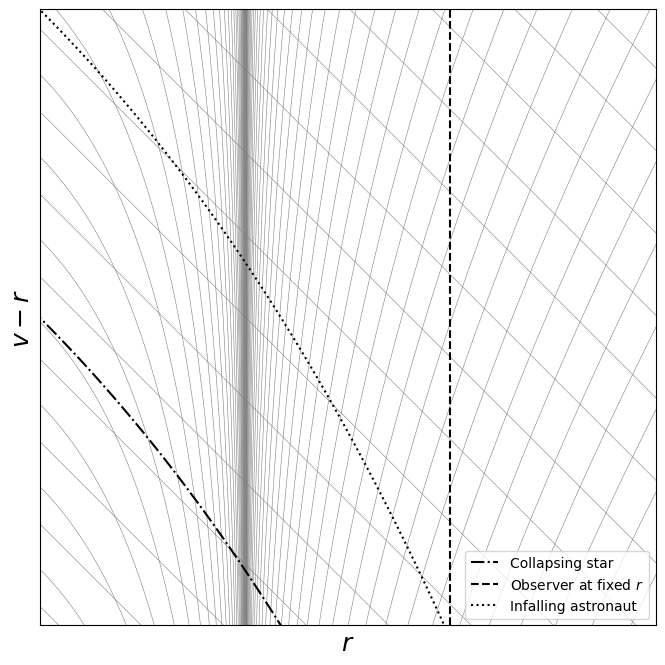
\includegraphics[width=4.8in]{EF_collapse.png}
\caption{Space-time diagram of spherically symmetric gravitational collapse in Eddington–Finkelstein coordinates. Null geodesics (grey) asymptotically approach vertical as they near the event horizon. Overlaid are the worldlines of three observers: the collapsing surface of a star, an infalling astronaut, and a static external observer. The diagram reproduces the essential elements of \citeauthor{Penrose1969}'s~\citeyearpar{Penrose1969} Figure 2, which formalised this scenario's causal structure.}
\label{fig:Sch-EF}
\end{figure}

Figure~\ref{fig:Sch-EF} shows the causal structure of the Schwarzschild geometry in the Eddington-Finkelstein coordinate frame, along with three timelike worldlines representing: (i) the surface of a spherically symmetric gravitationally collapsing star, (ii) an observer who remains at fixed radius $r$ outside the star, and (iii) an astronaut who departs from the external observer and falls inward. This figure is essentially the same as the one presented in \citet{Penrose1969}, and it reveals several features of the geometry that are especially clear in this reference frame.

First, the vertical line where the grey null rays appear to converge marks the event horizon at $r = 2Gm/c^2 \equiv 2m$ (in units where $G = c = 1$). At this radius, the outgoing null rays transition from propagating outward to propagating inward---yet the geometry remains smooth, and both the surface of the star and the infalling astronaut pass $r = 2m$ in finite proper time, with space-time remaining locally Minkowskian along their trajectories.

Second, infalling null lines appear at 45$^\circ$ in this frame. This is by construction: the Eddington-Finkelstein $v$-coordinate was defined to run parallel to ingoing null geodesics.

Third---and critically---past light cones of any point along the external observer's worldline \textit{never} intersect the event horizon. Neither the event at which the star's surface reaches $r = 2m$ nor the moment the astronaut crosses the same boundary is ever included in the past light cone of any external observer. No matter how long the observer waits or how close they are to the event horizon, every signal they receive from the star or astronaut always originates from a point outside the horizon. While they might imagine that collapse has ``already'' completed, the most recent observable evidence always shows otherwise.

Fourth (though equivalent in content to the third), the region outside the external observer's past light cone includes spacelike surfaces labeled as ``now'' that do extend through the horizon and down to $r = 0$, while still lying between the last received null signal and the horizon. This means that, depending on the foliation adopted, the external observer could either claim that the astronaut and star are already inside the black hole, or continue to claim indefinitely that they are both still falling toward it.

Fifth, this ambiguity is manifest in different spacetime slicings. According to Schwarzschild $t$-slicing, both the star's surface and the astronaut asymptotically approach the horizon as $t \to \infty$, never crossing it at any finite $t$. In contrast, in a $v - r$ slicing, the star's surface crosses the horizon ``before'' the astronaut. This multiplicity of valid foliations further exposes the coordinate dependence of any claim about what has ``already happened.''

The upshot of all these features is clear: from a strict operationalist perspective, where knowledge is confined to the past light cone and simultaneity outside that cone is treated as physically meaningless, the external observer can never conclude that collapse has completed. They can only affirm that each signal received so far originated from outside the horizon. Any inference about events occurring ``now'' beyond observational reach---whether that the crossing has happened or is still underway---is not just speculative but metaphysically undefined. Operational Relativism thus forbids any statement about whether the horizon has been crossed, even if such a statement feels intuitively or geometrically compelling.

If Operational Relativism is taken seriously, then it is logically invalid for the external observer to claim that collapse has ``already'' occurred. From their standpoint, every observable datum is consistent with the surface of the star and the astronaut remaining outside the event horizon indefinitely. Any stronger claim---e.g., that the black hole has already formed---smuggles in an unacknowledged ``now'' that violates the operationalist constraint.

Now let us examine how \citet{Penrose1969} described this same scenario:
\begin{quote}
    The observer on the rocket ship\ldots crosses freely from the $r > 2m$ region into the $0 < r < 2m$ region. He encounters $r = 2m$ at a perfectly finite time, according to his own local clock, and he experiences nothing special at that point. The space-time there is locally Minkowskian, just as it is everywhere else ($r > 0$).

    Let us consider another observer, however, who is situated far from the star. As we trace the light rays from his eye, back into the past towards the star, we find that they cannot cross into the $r < 2m$ region after the star has collapsed through. They can only intersect the star at a time \textit{before} the star's surface crosses $r = 2m$. No matter how long the external observer waits, he can always (in principle) still see the surface of the star as it \textit{was} just before it plunged through the Schwarzschild radius. In practice, however, he would soon see nothing of the star's surface---only a ``black hole''---since the observed intensity would die off exponentially, owing to an infinite red shift.
\end{quote}

This excerpt, together with the accompanying figure showing the star's surface and the rocket ship reaching the singularity at $r = 0$ in finite proper time, conveys a common inference: that while the external observer remains far from the star, the star nevertheless plunges through its horizon and becomes enclosed within a singularity. On this reading, the observer sees only a fading past image of the star because the real collapse has ``already'' occurred.

This inference is, however, premature. \logiclink{L4.7}{} It commits a modal fallacy---conflating what is inevitable in one frame (the star \textit{will} collapse) with what is already true in another (that it \textit{has} collapsed), despite the lack of any possible confirmation from that frame \citep{Curiel2017}. The confusion lies in mistaking an outcome guaranteed in proper time for an ontological fact in another frame. This is not a denial of the infaller's experience; it is a critique of projecting that inevitability across frames into a global ontological claim. Since the collapsing star's surface remains forever spacelike separated from the external observer, who remains at fixed $r > 2m$ for all proper time, there is no sense in which the observer can conclude that the horizon-crossing has ``already'' happened.

\logiclink{L4.6}{} The same error would be made in saying that someone you passed earlier in the hallway is now dead. It is true that their death is inevitable. But the last signal you received---the last interaction or memory---showed them alive. Unless a new signal arrives confirming otherwise, you cannot assert that they have ``already'' died.

Yet even this analogy is too generous. In the hallway scenario, confirmation might one day arrive. In the case of gravitational collapse, it never will. The event at which the star crosses the horizon lies outside the past light cone of all external observers---forever. No matter how long one waits, no signal can ever confirm that the horizon was crossed. The belief that collapse has ``already'' occurred is therefore not merely unconfirmed; it is unconfirmable even in principle. Any such claim imports a preferred foliation that the operationalist framework explicitly forbids.

In fact, another thought experiment reproduces the structural elements of spherical collapse exactly. Imagine a rocket ship with perfect insulation, capable of maintaining constant acceleration at $1g$ indefinitely. Before launch, you place a hot cup of coffee on a desk aboard the ship, next to a clock that displays the arctangent of proper time, and you stick a thermometer in the coffee. The ship continuously transmits a laser-focused signal back to Earth, reporting both the coffee's temperature and the clock reading.

From Earth's perspective, the signal quickly becomes redshifted and fades from view. But in principle, the signal remains forever observable. Its contents show that the coffee's temperature asymptotically approaches thermal equilibrium with its surroundings, and the clock reading asymptotically approaches $\pi/2$---a finite number---though both limits are only reached after infinite time.

This scenario precisely mirrors the case of gravitational collapse. Just as the collapsing star's radius appears to asymptotically approach $r = 2m$ in the infinite future of the external observer, so does the coffee's temperature appear to asymptotically approach equilibrium. And just as the star's proper time appears to remain finite, the signal from the rocket shows that the clock asymptotically approaches a finite value.

But crucially, no one would infer from this that there is some unobservable ``real'' moment when the temperature hits equilibrium exactly, or when the clock suddenly surpasses $\pi/2$. We do not imagine that the ship ``crossed'' some hidden threshold in reality, beyond which a different geometry takes over. \logiclink{L4.8}{} The conclusion we are entitled to draw---based on observable evidence---is simply that the temperature and clock reading will forever continue to approach those limits. No observer, regardless of patience or ingenuity, can ever confirm that the system has reached the limit---only that it continues to approach it. This epistemic boundary is structural, not technological.

Likewise, from the external observer's perspective, the only justifiable statement is that the star's surface continues to approach the event horizon in finite proper time, and the signal from it continues to redshift and fade. \logiclink{L4.11}{} Any claim that the horizon has already been crossed is not only unverified---it is unscientific.

The only difference between the two scenarios is that in the thought experiment we know that in reality the clock never will read anything more than $\pi/2$, and the temperature will not drop below the finite value it reaches in thermodynamic equilibrium. We know this because these are facts of the experiment's design. But from a purely observational perspective, for example in the case where the record of the experiment has been lost on Earth and a later civilisation discovers the signal by chance, those observers cannot be so certain that the asymptotic limits they observe will also be the actual end state, or if the temperature and proper time will in reality continue beyond the values that are observable.

In both cases, all available information indicates continued approach toward an asymptotic limit. This causal structure remains intact not only in classical general relativity but also in standard semi-classical models, including those incorporating Hawking radiation \citep{Visser2003, Wald1994}.\footnote{This analysis is restricted to classical and semi-classical models of collapse. While full quantum gravity may introduce qualitatively new phenomena, such proposals remain speculative and do not alter the causal structure or asymptotic observability constraints described here. Even semi-classical treatments such as Hawking radiation retain this asymptotic character from the perspective of any external observer.} In these models, the collapse exterior remains observationally indistinguishable from classical asymptotic approach for any finite external time. Thus, the operational inaccessibility of horizon-crossing events persists even when quantum effects are included---at least up to the threshold of a full quantum gravity theory.

In no other domain of physics do we allow ourselves to infer that an unobservable event \textit{has definitely} happened simply because the theory predicts it \textit{will eventually} happen. \logiclink{L4.9}{} This reflects a striking epistemic asymmetry: in nearly all domains of physics, asymptotic behaviour is treated with caution, and no claim of state completion is made unless confirmable. Yet in black hole physics, we routinely assert a completed ontological transition at the very point where causal verification is forever precluded. Only in the case of black holes have physicists convinced themselves that something real and physically distinct happens at that limit---even though no observation could ever confirm it.

This thought experiment clarifies the modal fallacy in the standard picture of gravitational collapse to a black hole. \logiclink{L4.10}{} The causal structure of the Schwarzschild geometry is consistent with both a description in which the star's surface has already plunged beneath its horizon and one in which the star is asymptotically approaching the horizon and will continue to do so indefinitely. And since the horizon-crossing event never enters the past light cone of any observer anywhere in the outside universe---even one who is mere centimetres away from the collapsing star---this ambiguity about what has ``already'' happened and what is still to come in the future \textit{must} always remain. The physical description of gravitational collapse is fully consistent with a scenario that is equivalent to the coffee's temperature asymptotically approaching thermodynamic equilibrium with the rocket ship's cabin while the ``time'' onboard the ship approaches~$\pi/2$. In that description, the collapsing star's radius asymptotically approaches $r=2m$, while its proper time asymptotically approaches the finite value it will reach at $r=2m$, and in reality this takes place over infinite time in all external frames. Since both descriptions are valid, and observations can never confirm that the horizon has been reached, concluding that the horizon has already been reached is a logical fallacy---one that depends on the unacknowledged introduction of a preferred \textit{now} in order to support the desired metaphysical conclusion.

In fact, this highlights the importance of maintaining a strict operationalist perspective when a preferred foliation has not been rigorously justified and consistently accounted for in physical descriptions. For if one begins with an operationalist framework but then later interprets certain spacelike-separated events as ``really'' concurrent within a dynamical picture, this is logically inconsistent. And from a strict operationalist perspective, it is meaningless to speculate whether black holes have already formed within our universe or whether they are still asymptotically approaching their horizons, since all we can know is that the collapsing stars were still larger than their event horizons at the times we are now observing---and they always will be.

And if we reject operationalism and wish to speculate about which ``now'' is really true while still maintaining Einstein's operational definition of simultaneity, we are forced to accept the block universe interpretation, in which all events \textit{zare} at once real, and in which no events \textit{exist}. In that case, from the external observer's perspective, the gravitational collapse both \textit{iz} and \textit{iz not} already complete---just as all events throughout eternity \textit{zare} real at once, within the non-existing block. Objectively speaking, if we are to rigorously maintain logical consistency, this is the closest we can come to justifying the standard conceptual model of gravitational collapse to a black hole. \logiclink{L4.12}{}

The outcome is stark. General relativity permits two ontologically incompatible collapse interpretations---finite-time and asymptotic---yet offers no justification for preferring either. From a strict operationalist perspective, the metaphysical claim that the collapse has ``already'' completed is not merely unverifiable but scientifically meaningless. From a realist standpoint, the asymptotic alternative remains observationally indistinguishable and just as valid, rendering the assertion of completed collapse potentially false. \logiclink{L4.13}{} In either case, the inference fails: the standard collapse model, if asserted as fact, is either epistemically unjustified (if one grants it the benefit of doubt), or objectively false (if the asymptotic interpretation is correct and complete), and in both cases incompatible with scientific standards. Thus, objectively, the standard collapse model lies somewhere between being potentially true---but then scientifically meaningless---and \textit{false}. Any attempt to assert it as fact necessarily invokes additional, unobservable ontological commitments not grounded in causal structure or accessible evidence.

\subsection{The Smuggled Now in Cosmology}\label{sec:4.3.2}
\noindent\textit{Supports Logic Map B nodes: \hyperref[appendix:III3]{[III3]}, \hyperref[appendix:III4]{[III4]}, \hyperref[appendix:V1]{[V1]}, \hyperref[appendix:V2]{[V2]}, \hyperref[appendix:IV3]{[IV3]}.}

\vspace{4pt}

\logiclink{L4.15}{} To model the evolution or large-scale structure of a coherent universe, it is necessary to assume a universal now: a global foliation of space-time into spatial hypersurfaces ordered by a shared time parameter. In a Lorentzian space-time, this ``now'' corresponds to a foliation that defines noumenally concurrent sets of events. These events are generally not simultaneous in arbitrary reference frames, nor does proper time in those frames normally align with the cosmic time parameter that structures the foliation. As \citet{Eddington1920} noted in the earliest days of relativistic cosmology, before it was even known that the universe extended beyond a sea of stars and nebulae:
\begin{quote}
The world taken as a whole has one direction in which it is not curved; that direction gives a kind of absolute time distinct from space. Relativity is reduced to a local phenomenon; and although this is quite sufficient for the theory hitherto described, we are inclined to look on the limitation rather grudgingly. But we have already urged that the relativity theory is not concerned to deny the possibility of an absolute time, but to deny that it is concerned in any experimental knowledge yet found; and it need not perturb us if the conception of absolute time turns up in a new form in a theory of phenomena on a cosmical scale, as to which no experimental knowledge is yet available. Just as each limited observer has his own particular separation of space and time, so a being coexistive with the world might well have a special separation of space and time natural to him. It is the time for this being that is here dignified by the title `absolute'.
\end{quote}

The idea that a cosmic now exists---flowing \textit{outside the confines of our personal experience} of time and space---poses a conceptual challenge for models grounded in strict operationalism. A cosmic now implies that our individual experiences of simultaneity and duration are not globally valid: events that appear synchronous to us may not be simultaneous in this deeper structure. This seems at odds with the operationalist principle that noumenally simultaneous events are those that occur synchronously within one's own proper causal past.

Historically, this conflict was resolved by assuming that the average worldlines of matter form a coherent bundle or ``pencil'' of geodesics. Weyl's principle formalises this intuition. The pencil metaphor is especially useful: not only do the worldlines form a non-intersecting bundle, but its \textit{sharpened tip} corresponds to the observer's past light cone, with more distant geodesics intersecting earlier in cosmic time. This ensures compatibility with the causal structure of relativity, while also defining a shared state of rest and a consistent spatial hypersurface across space-time---one that expands backward in time from the tip.

Weyl's pencil provided a particularly apt visualisation of \citet{Einstein1917}'s original cosmological model, which featured a finite spherical space of constant radius. But the metaphor remains powerful in expanding Friedmann-Lemaître-Robertson-Walker (FLRW) cosmologies as well. In such models, the comoving geodesics remain orthogonal to each spacelike hypersurface of constant cosmic time, and the universe's expansion is described by a time-dependent scale factor that preserves this orthogonality. Thus, the same topological structure persists even as space expands---a coherent foliation underwrites cosmological description at all scales.

It is in this sense that \citet{Eddington1920} characterised the time dimension as the one direction in which the four-dimensional world is not curved, as this pencil of geodesics sets up a common proper time in the average rest frame of galaxies within the universe. Eventually, \citet{Hubble1929} discovered his redshift-distance relation, in which this ``average motion'' concept was readily apparent. For the observations did not show that the distances to galaxies were tightly correlated to their apparent redshifts, with scatter explained by systematic measurement uncertainty alone. Rather, the observed redshifts were taken to be a \textit{combined} measurement of both Doppler shifts due to the galaxies' radial motion \textit{through} space (this being the cause of scatter about the best-fit line) and a \textit{cosmological redshift} (captured by the average trend in the data) that \textit{progressively accumulates} along the photons' paths through expanding space. Therefore, if distant galaxies were all perfectly stationary relative to us within expanding space, and we could measure their distances and redshifts precisely, we expect that the data would show a precise redshift-distance relation due to increased accumulation of redshift along longer paths through the expanding universe.

It is important to be clear that according to this expanding universe explanation of the phenomenon, the redshift must not be confused with an effective velocity, nor any other property directly related to the emission \textit{source}. The cosmological redshift is, under the standard interpretation of the phenomenon, a \textit{cumulative effect} that grows \textit{while} photons travel through expanding space---which, in the case of continuous cosmic expansion, is therefore larger the further the galaxy's original distance was from us at the time of emission.

Now, the standard model we use to describe this phenomenon is based on four kinematical principles and one dynamical principle, which must be assumed in a particular order \citep{Robertson1933,Walker1937,North1965}. First, we assume based on the galaxies' apparent motions that their average state of rest can be represented by a coherent bundle of geodesics measuring the proper time $t$ of matter. Second, that the space $t=\mathrm{const.}$ is orthogonal to this congruence of geodesics. Third, that the space so-defined is isotropic. Fourth, that this space is also homogeneous. And fifth, that the spatial geometry evolves according to a multiplicative scale factor $a(t)$, the form of which is constrained by the requirement that the kinematical line-element defined through the first four assumptions be a solution to the Einstein field equations.

These basic principles give us the standard Friedmann-Lemaître-Robertson-Walker (FLRW) model of cosmology \citep{Friedmann1922,Friedmann1924,Lemaitre1927,Robertson1935,Walker1937}. The form of $a(t)$ given by Einstein's equations depends on energy densities of fluids (matter, radiation, dark energy) which are assumed to be maximally symmetric on large scales, in accordance with the assumed isotropy and homogeneity of space. Therefore, by observing distant phenomena and measuring the precise form of expansion through its cumulative influence as light from distant sources made its way to us through variably expanding space, we are able to estimate the amounts of different energy fields within our universe and estimate properties such as its age and what its eventual fate will be.

Now, it is worth noting that cosmological observations do not grant direct access to our entire causal past, but rather the information is fairly tightly constrained to our past light cone. Through physical models, we can infer past states of objects we see, such as properties of constituent galaxies we now see merging, but generally speaking when observing a galaxy that is, say, only 10 million light years away, whose past worldline extends some 13 billion years into the past \textit{within} our past light cone, we have a much better idea of its \textit{present} state than of its detailed formation history or its first several billion years. The best knowledge we have of the formation of early galaxies comes from studying galaxies that are so far away that, due to the finite speed of light, we now see them forming. But from our past light cone's worth of observations, and by employing the full space-time metric of cosmology, we do our best to fill in the details not just of the sharpened edge of the pencil of geodesics, but even the fully unsharpened pencil and often even beyond that, extrapolating the cosmic foliation both within and beyond our observable universe, modelling the bundle of geodesics up to the cosmic present.

For example, while we know that the cosmic microwave background (CMB) photons travelled 13.8 billion light years through variably expanding space from the edge of our observable universe (since they've travelled at light speed for 13.8 billion years), through our empirically constrained density parameters and expanding universe model we infer other values of interest as well. At the time the CMB photons were emitted by the surface of last scattering, when the expansion of space had finally caused their energy to drop sufficiently enough that the matter and radiation within it decoupled from a plasma, the CMB photons we \textit{now} observe were at an isotropic radial distance of only 42 million light years from our current location in space. But because those initially 42 million light years of space have been expanding as the CMB photons travelled \textit{through} them, the full distance they ended up traversing was 13.8 billion light years. Initially, while space was still much smaller, they covered a greater proportion of those 42 million light years, while more recently each of those initial light years of space had grown by a factor of $\sim1000$, so they took that much longer to traverse. On the other hand, the present distance to the last scattering surface, which is roughly the present size of the observable universe, is 46 billion light years. Every galaxy we see as we look out through space and back in time \textit{now} lies within this radius.

Throughout this period, from the time of last scattering when the universe was only 370,000 years old to its present 13.8 billion years, the universe continually expanded, its temperature cooled through expansion-induced redshift of CMB photons, its matter and radiation densities decreased while the dark energy remained constant or slowly varied, and the matter, now decoupled from radiation and seeded by slight inhomogeneities that existed already at last scattering, quickly clumped together to form a cosmic web of galaxies and clusters separated by vast voids. We know that the universe was an almost perfectly homogeneous blackbody at the time of last scattering because the CMB that decoupled from matter when the photons had sufficiently redshifted through the first 370,000 years of expansion remains a nearly perfect blackbody. And we know it contained slight inhomogeneities because the CMB photons bear this mark as well: a near-scale invariant anisotropy spectrum on the order of $\Delta T/T\sim10^{-5}$, due to photons emerging from slightly overdense regions being gravitationally redshifted and photons from slightly underdense regions being gravitationally blueshifted relative to the average---a phenomenon known as the Sachs-Wolfe effect \citep{Sachs1967}.

While the CMB's blackbody spectrum confirms that the early universe \textit{was} in thermal equilibrium at the time of last scattering, this alone is not the full story. The photons we observe today have travelled 13.8 billion years along the edge of our past light cone, \textit{through a dynamically expanding universe that continually redshifted them along the way}. The fact that we now observe this thermal spectrum to be precisely isotropic---after accounting for known secondary effects---places extraordinarily strong constraints not only on the conditions \textit{at} recombination, but also on the geometry and expansion history of space \textit{throughout the period} since then.

\logiclink{L4.16}{} If expansion had not been isotropic, the photons we observe today would have originated from different initial proper distances, and the last scattering surface would not form a perfect 2-sphere. Instead, it \textit{would appear distorted}: in directions where the overall expansion was slightly less, we would see photons emitted at larger initial distances than 42~Mly; in directions with faster expansion, from smaller ones. These distortions would break the observed angular symmetry of the anisotropy pattern, shifting the angular size of acoustic peaks and distorting the power spectrum from what is described by our model---which assumes perfectly uniform, isotropic expansion. These expansion anisotropies would also introduce redshift anisotropies---true cosmological redshift differences arising from differential expansion along the photons' anisotropic paths---which we do not observe.

We see none of these indicators that there has been any anisotropic expansion since last scattering. The angular scale of anisotropies is consistent across the entire sky, and the redshift to the last scattering surface is isotropic to at least one part in $10^5$ after accounting for secondary effects like the Doppler dipole due to our own motion through space and gravitational redshifts due to the Sachs-Wolfe effect, the integrated Sachs-Wolfe effect, and weak lensing \cite{Sachs1967, Aghanim2020}. The standard model \textit{assumes exactly} this structure: that the last scattering surface is an exact 2-sphere, and that space has expanded isotropically in all directions ever since. 
This assumption is not only consistent with observation---it is tightly constrained by it: if the magnitude of expansion anisotropy exceeded $\Delta a / a \sim 10^{-5}$, it would have left imprints in the CMB temperature anisotropies that we \textit{do not observe}.

Here, the distinction between a coordinate slicing and a physical foliation becomes crucial: the RW slicing is not merely a charting convenience, but a \textit{geometrically determined} structure---\textit{uniquely fixed by the condition of isotropic expansion}.\footnote{For broader philosophical discussions of preferred foliations in cosmology, see \citet{Sklar1995}, \citet{Maudlin2007}, and \citet{ellis2006}. These works explore the conceptual significance of slicing structures in both classical and relativistic frameworks.} The standard model fits the data \textit{precisely} and bounds any possible deviations from \textit{perfectly} isotropic expansion to extraordinarily high precision \textit{within the observable universe}.

It is worth pausing to reflect on the significance of this result. While we've modelled the expansion of our universe as being perfectly isotropic, that isotropy was never guaranteed---and certainly not to a precision of one part in $10^5$, a level of symmetry far beyond what any a priori physical principle would demand. In order for the expansion redshifts of CMB photons all across the sky to be so precisely uniform, either the expansion rate since recombination \textit{really must} have been precisely isotropic, or expansion anisotropies along any two lines of sight anywhere in the sky would have to conspire to produce precisely the same cumulative redshift \textit{after travelling 13.8 billion light years} through anisotropically expanding space. 

This isotropy does not merely confirm uniform expansion rates; it confirms the existence of a coherent global foliation. For such isotropy to be observed from our location, the universe must have expanded equally in all directions throughout cosmic time. The empirical isotropy of redshift thus provides observational grounding for the existence of the RW slicing itself---not just as a coordinate frame, but as a privileged physical structure. To claim that the isotropy of CMB redshift is merely a coordinate artefact or model fitting artefact would require that observational isotropy arise from asymmetric expansion histories along every line of sight, precisely cancelling to one part in $10^5$. This is not just an implausible coincidence---it would constitute an extraordinary observational coincidence without precedent in physics. \textit{The only alternative to a} genuine \textit{cosmic foliation is a redshift conspiracy without precedent in physics}.

However, independent observations confirm that the precise form of expansion along different lines of sight has also been isotropic. Baryon Acoustic Oscillation measurements provide a standard ruler at multiple redshifts, while Type Ia supernovae serve as standard candles, enabling detailed reconstruction of the expansion history along many lines of sight. \logiclink{L4.17}{} The remarkable agreement of these independent tracers with the standard model \textit{across all surveyed directions} confirms that not only the integrated redshift, but the full dynamical history of expansion, has been isotropic to high precision \citep{ellis2006,clarkson2010}.

Together, these observations provide not merely circumstantial support, but precise \textit{scientific verification} of the basic principles of the standard model. Therefore, cosmological observations have not only confirmed that we live in a uniformly expanding universe, but they've precisely confirmed the cosmic time foliation which describes a cosmic now and associated ``preferred'' state of rest in our universe, as assumptions on which the standard model was based. What began as a pragmatic idealisation---used to model the large-scale coherence of the universe---has turned out to describe the universe's actual structure with extraordinary fidelity. \logiclink{L4.14}{} The cosmic now, initially introduced as a modelling convenience, is not merely a smuggled artefact. It is a hypothesis that has been empirically corroborated to extraordinary precision according to the basic logical structure of science. And with that, the cosmic present has transitioned from an abstract convention into an empirically grounded feature of physical reality. \textit{This outcome exemplifies the fundamental logic of science}: a hypothesis originally introduced to simplify modeling has been tested and confirmed across multiple observational channels, thereby elevating it from assumption to a precisely verified feature of our universe.\footnote{One might hope for a more principled justification of cosmic time within the theory itself. For example, appealing to the spirit of Mach's principle, one might speculate that cosmic time could emerge from the average motion of matter in the universe---thus preserving a sense of relational grounding. But this idea, while rhetorically appealing, is logically tautological: in order for matter to have a coherent average rest frame, it must coherently exist to begin with; in order for it to \textit{move} at all, whether in a common way or not, matter must already exist---and relational properties cannot precede the relata; emergence cannot precede existence.}

\logiclink{L4.18}{} In fact, not only have our cosmological measurements confirmed indirectly through model verification that this cosmic \textit{now} exists---that our universe is \textit{now} 13.8 billion years old---but we have also \textit{directly measured our velocity} relative to the preferred state of rest, through the CMB dipole anisotropy, as $v=(369.82\pm0.11)$~km/s towards the constellation Crater \cite{Aghanim2020a}.

\section[The Collapse of Logical Coherence in Relativity]{The Collapse of Logical Coherence in Modern Relativistic Physics}\label{sec:4.4}
\noindent\textit{Supports Logic Map B nodes: \hyperref[appendix:III2.1]{[III2.1]}, \hyperref[appendix:III2.2]{[III2.2]}, \hyperref[appendix:III3]{[III3]}, \hyperref[appendix:III4]{[III4]}, \hyperref[appendix:V1]{[V1]}, \hyperref[appendix:V2]{[V2]}.}

\vspace{4pt}

When working on the problem of cosmology, we describe a well-defined cosmic ``now'' that has evolved from the Big Bang, through an inflationary epoch, recombination, and the formation and evolution of structures like voids and filaments, within which individual galaxies like our own form. When working on the problem of gravitational collapse within that same universe, we shift frames entirely---basing our standard inference on a preferred foliation that leads to the paradoxical result that space-time singularities ``now'' \textit{exist} at the centres of vacuous space-time regions, where an isotropic radial dimension of \textit{time} ``exists,'' through which particles continue to stream as if the interior is a four-dimensional arena they can \textit{move through}, even as the space outside is thought to evolve in cosmic time. And when we speculate about closed timelike curves, wormholes, or superluminal travel, we shift from this hybrid view, invoking an enduring space-time in which all events \textit{exist}, and time travel is imagined as a kind of navigation through the block as it ``now'' endures. As shown in \S~\ref{sec:4.3}, these interpretive shifts are not merely heuristic choices, but logically incompatible frameworks selectively invoked in different domains---exposing a structural failure to consistently distinguish operational from metaphysical reasoning. Each of these interpretive shifts presupposes a different ontological structure, yet all are deployed within the same theoretical framework---without reconciliation or even acknowledgment.

\logiclink{L4.19}{} These interpretive moves are not derived from theory. They are not mandated by relativity. They are not even consistent with each other. They reflect a pattern of selective realism and interpretive sleight-of-hand that has allowed modern physics to avoid confronting the internal contradictions of its frameworks---contradictions that become glaring once the interpretive choices are lined up side by side.

Let us consider cosmology. In \S~\ref{sec:4.3.2}, after carefully setting up the operational framework with sharpened pencil of geodesics representing our past light cone, I eventually---intentionally---lapsed into the common manner of describing our observable universe as an evolving space, one that had a radius of 42 million light years at the time of last scattering, when all events that occurred within it actually are contained within our past light cone, to a space with radius 46 billion light years today, which lies completely outside our past light cone. All the galaxies and the CMB in our observable universe, the images of which we now observe  through photons that travelled along our past light cone, are more accurately represented by an unsharpened pencil of geodesics that extends from the time of last scattering to today. Each of these geodesics intersects our past light cone at a single point---the event which is presently visible to us.

Eventually, this slip into common language was justified through the explanation that the cosmological evidence actually strongly supports the notion that we \textit{do} live in a well-defined, enduring, three-dimensional, uniformly expanding universe, with an associated, physically measurable rest frame. In this, we found that while relativity alone indicates that a preferred rest frame could never be observable even if one exists, our universe actually provided a mechanism that makes the measurement possible, via the physical processes that produced the CMB and the geometric structure of its uniform expansion over cosmic time. 

But while this language used to describe the evolution of the universe is indeed common, few physicists or philosophers are comfortable acknowledging that the cosmological evidence has turned out to strongly support the model's foundational kinematical assumptions of absolute cosmic time and uniform expansion---or the significant and surprising fact, against pure relativity-based expectations, that the universe actually provided a physical mechanism through which we can---and do---precisely measure our own velocity through it.

While physicists and philosophers alike often express a desire for coherence, in practice the pursuit of internal consistency has too often been subordinated to pragmatic aims. Models are assessed for their utility, not for the consistency nor the extent of the metaphysical commitments they are making. Interpretive frameworks are swapped without regard for whether their underlying assumptions cohere with one another---or with the theory itself. 

In what follows, we use the term \textit{metaphysical commitment} to refer to any interpretive assumption that goes beyond strictly observational claims and posits something about what exists, occurs, or endures in physical reality. Such commitments are distinct from operational descriptions, which only concern what can be measured or inferred from causal structure. The key problem we will expose is not that physicists make such commitments, but that they do so inconsistently and often without recognising them as such.

For a specific example of this, let us return to the problem of gravitational collapse. As explained in \S~\ref{sec:4.3.1}, the classic illustration of spherically-symmetric collapse to a Schwarzschild black hole in the Eddington-Finkelstein coordinate frame selects one preferred slicing to describe the dynamical process while ignoring the alternative slicing which is both operationally indistinguishable and offers an equally valid description of the dynamical unfolding of events in reality from the perspective of the mathematical theory.

\begin{figure*}[t]
\centering
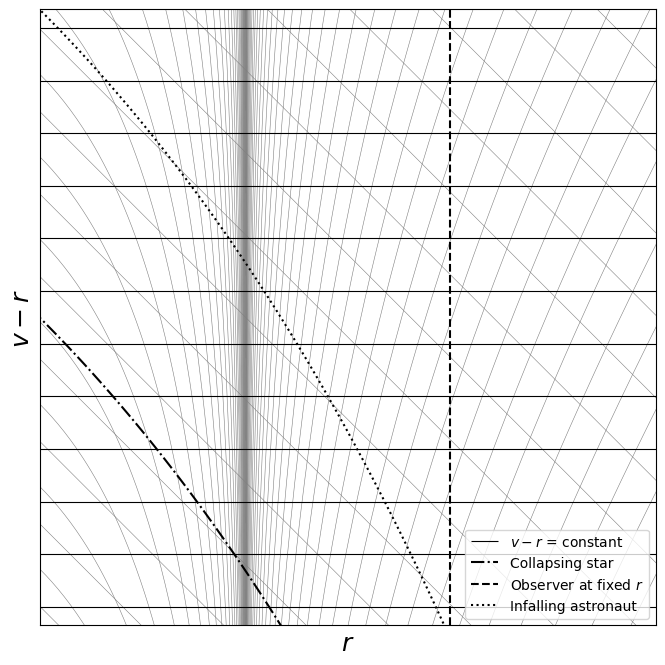
\includegraphics[width=3.25in]{EF_collapse-vr.png}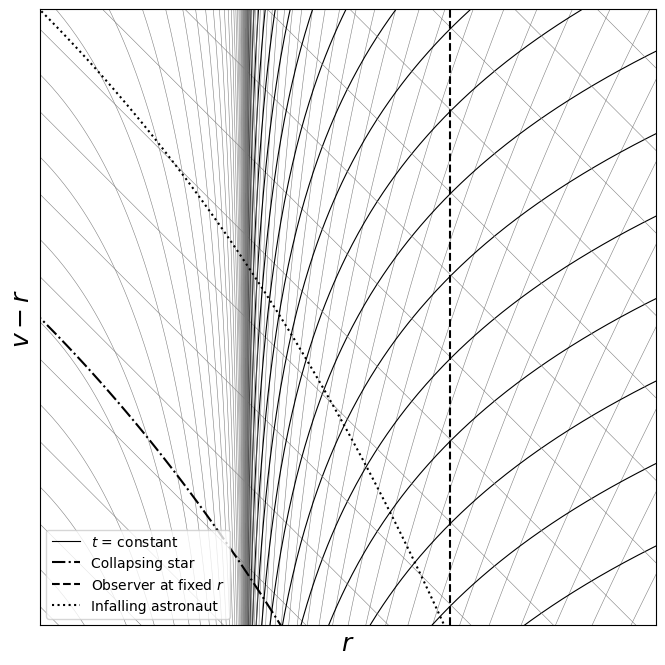
\includegraphics[width=3.25in]{EF_collapse-t.png}\\
\hspace{0.1in}(a)\hspace{3.25in}(b)
\caption{The same Eddington–Finkelstein diagram as in Figure~\ref{fig:Sch-EF}, now overlaid with two distinct foliations. Solid black lines depict (a) hypersurfaces of constant $v-r$ and (b) hypersurfaces of constant Schwarzschild coordinate time $t$. These contrasting slicings illustrate how coordinate choices affect the apparent simultaneity and interpretation of collapse, even though they share the same causal structure and describe the same underlying space-time geometry.}
\label{fig:Sch_EF-foliated}
\end{figure*}

To see clearly how one and the same geometry, considered in the same reference frame, can be used to describe the unfolding of two ontologically distinct dynamical processes, refer to Figure~\ref{fig:Sch_EF-foliated}, which is the same space-time diagram shown in Figure~\ref{fig:Sch-EF} above, but here showing two explicit spacelike foliations of the geometry depicting the manner in which sequences of events may be interpreted to unfold in reality. \logiclink{L4.20}{} Since general relativity does not specify any preferred foliation, an objective, ontologically neutral interpretation of gravitational collapse---consistent with operational relativism---cannot logically commit to any single subset of the union of possible realities.

Figure~\ref{fig:Sch_EF-foliated}(a) corresponds to the classic gravitational collapse picture, in which complete collapse occurs in finite time, not just in the proper frame of the star but from the perspective of external observers as well who define ``now'' according to this foliation. According to this picture, in finite ``time'' the star plunges beneath $r=2m$ and later collapses all the way to $r=0$, where it forms a massive singularity. A little while later, the infalling astronaut, who left the fixed external observer and dove towards the collapsing star before it had even reached its horizon, reaches the horizon as well, and a while later the astronaut too has fallen all the way to the singularity at $r=0$. Meanwhile, the observer at fixed $r>2m$ forever sees both the surface of the star and the light from the rocket ship as they shone towards him ``before'' they plunged beneath the horizon. No matter how long the external observer waits, he will always in principle be able to see both the star and the rocket ship as they \textit{were} ``before'' reaching the horizon, even though a massive singularity is all that \textit{actually remains} of the two---though in practice both signals would soon become too redshifted to be observable.

Figure~\ref{fig:Sch_EF-foliated}(b) depicts a fundamentally different unfolding of events. In this case, both the surface of the star and the infalling astronaut still reach $r=2m$ in finite proper time, but here they no longer do so one after the other, but simultaneously, both asymptotically approaching $r=2m$ as ``time'' goes to infinity. In this picture, gravitational collapse is a purely asymptotic process when described from anywhere in the universe: the event horizon never forms, and both the collapsing star and the infalling astronaut remain forever well-defined spatially extended objects that \textit{always} ``still exist'' in ``space.'' The peculiar feature of this picture is that when infinite time has elapsed in reality, only finite proper time has elapsed in all infalling reference frames. Therefore, when all infalling matter simultaneously reaches the event horizon at the end of time, infalling observers in their local frames find themselves at well-defined space-time points (likely wondering what comes next). 

This ambiguity is familiar in canonical formulations of GR, where the ``problem of time'' arises precisely because the Einstein equations admit many foliations, none of which are physically preferred \citep{isham1993}.\footnote{Some philosophical approaches, such as perspectival realism and structural realism, attempt to accommodate such ambiguities without fully resolving them (e.g., \citealt{Ladyman2007}, \citealt{Massimi2012}). However, these frameworks still presuppose consistency within a given interpretive stance---something current relativistic practice fails to maintain.} The ADM formalism, for example, defines a 3+1 decomposition in terms of lapse and shift, but this mathematical structure does not fix any ontological interpretation of time evolution \citep{arnowitt1962,arnowitt2008}. From an operational perspective, neither picture in Figure~\ref{fig:Sch_EF-foliated} can be definitively claimed to be the ``true'' description of reality. Therefore, from an objective mathematical standpoint it is best to leave the foliated hypersurfaces off the diagram entirely, as in Figure~\ref{fig:Sch-EF}; but in practice our minds tend to fill in the horizontal lines of Figure~\ref{fig:Sch_EF-foliated}(a), smuggling in unwarranted ontological commitments under the guise of neutrality.

From the standpoint of strict operational relativism, whether everything that ever falls into the black hole reaches its event horizon sequentially or all matter simultaneously reaches the horizon at the end of time, is essentially to be considered meaningless---a question of pure metaphysics. From the standpoint of strict operational relativism, all that matters is that the external observer can never confirm that either the star or the astronaut has ever ``already'' reached the horizon, as they both always appear to \textit{have been} still approaching it when the presently observed signal was sent. Importantly, this is true from the relative perspective of \textit{every} external point in space, no matter how close it is to the surface of infalling matter. From the perspective of the \textit{entire} external universe---all points in space surrounding the collapsing star, forever---what matters is that the collapsing matter forever remains ``still collapsing'' at the boundary of their past light cone.

\logiclink{L4.21}{} The choice to interpret gravitational collapse as completing in finite time is not mandated by the theory. It is not an observational inference. It is a metaphysical commitment---one that ignores an equally viable alternative description of the same geometry. And yet this commitment has driven decades of research, from black hole thermodynamics to information paradoxes, all while claiming ontological neutrality.

And this is exactly where the logical breakdown in standard black hole physics extends into metaphysical overreach. Because, after committing to the first picture of collapse over the second, having smuggled an unjustified sense of ``now'' into the concept, physicists commonly conclude that black holes must now exist in reality, as products of dynamic gravitational collapse. And on the basis of that commitment, while conveniently forgetting that collapse \textit{never} completes and the event horizon \textit{never} forms within \textit{any} external observer's past light cone, they derive consequences of the complete black hole's existence in reality and worry about observable problems that would then consequently emerge.

For example, while the massive singularity of a spherically symmetric black hole remains behind an event horizon, a rotating Kerr black hole with realistic angular momentum could have a singularity outside the event horizon. The potential existence of such ``naked'' singularities would be deeply problematic if they existed in our universe, so \citet{Penrose1969} proposed a cosmic censorship conjecture that would ensure these naked singularities do not arise. However, the problem is significantly diminished when noting that not only does the singularity never emerge, but even the event horizon has never formed, and all the matter within the collapsing black hole remains forever located in well-defined space, when considered from a pure, objective operational standpoint.

Similarly, on the basis that event horizons already exist, \citet{Hawking1975} showed that black holes must actually emit blackbody radiation. And since this radiation contains none of the detailed information about the objects that formed the black hole in the first place, but is determined solely on the black hole's overall mass, angular momentum, and charge, \citet{Hawking1976} reasoned that this creates a paradox because information is lost. But \textit{from the perspective of the entire outside universe}, the event horizon never forms in the first place, so the black hole never does radiate into the observable universe. 

\logiclink{L4.22}{} Each of these problems is manufactured on the false premise that the black hole has come to exist in the causal past of the outside universe. If we acknowledge first that the black hole has never ``already'' formed, that in fact the collapsing star has never even reached its event horizon ``already'' in any meaningful sense from any external point of observation, then from a purely causal standpoint it is clear that the black hole can never radiate into the observable universe, since that radiation can only come after the formation of the event horizon within the observable universe, which never happens. (This is, again, the same modal fallacy diagnosed in \S~\ref{sec:4.3.1}: a confusion between what is inevitable in one frame and what has already occurred in another. The assertion that collapse has already completed---despite eternal causal opacity---depends entirely on privileging a particular foliation without justification, and drawing metaphysical inferences that outrun what the formalism demands.) And there can never be a ``naked'' singularity since external observers must always find that it last remained shrouded in the ``clothing'' of a still-collapsing star.

What this example reveals is that the problem in modern relativistic physics is not merely the inconsistent use of ``now,'' nor the casual shifts between interpretive frameworks. It is the failure to recognise that each such shift entails a substantive \textit{metaphysical} commitment---one that is routinely denied, downplayed, or mischaracterised as agnostic or purely operational. \logiclink{L4.24}{} The issue is not that physicists make metaphysical assumptions; it is that they make them while sincerely believing they have not. They treat their conclusions as if they arise from an ontologically neutral theory, even when those conclusions depend on unacknowledged ontological commitments. \logiclink{L4.25}{} This is not a principled refusal to do metaphysics, but a failure to recognise that metaphysics has already been done---often implicitly, and inconsistently, and in ways that make even ontological deflationism untenable once the contradictions are laid bare. \logiclink{L4.23}{} This contradiction---between operationalist rhetoric and realist practice---is not a minor misstep. It is structural. It is epistemically indefensible, violating the core principles of falsifiability and testability. It is ontologically incoherent, embedding contradictory assumptions without reconciliation. And it is methodologically corrupting, generating paradoxes not from empirical anomalies but from metaphysical overreach misrepresented as neutral inference. And it demands a structural reform. Absent such reform, the discipline risks mistaking explanatory convenience for ontological coherence---treating incompatible commitments as if they form a unified picture of reality, when in fact they undermine the very integrity of physical explanation.

Only by recognising that interpretive consistency is not optional---but a condition of scientific integrity---can we restore coherence to our understanding of space-time, gravity, and physical reality. While \citet{Maudlin2007} has criticised the interpretive inconsistency of modern relativistic physics, the contradictions exposed here point beyond diagnosis---toward the necessity of structural ontological reform.

\section[Selective Realism and the Fear of Ontology]{Operationalism, Selective Realism, and the Fear of Ontology}\label{sec:4.5}
\noindent\textit{Supports Logic Map B nodes: \hyperref[appendix:I4]{[I4]}, \hyperref[appendix:III2.1]{[III2.1]}, \hyperref[appendix:III2.2]{[III2.2]}, \hyperref[appendix:III4]{[III4]}, \hyperref[appendix:IV1]{[IV1]}, \hyperref[appendix:IV2]{[IV2]}, \hyperref[appendix:IV3]{[IV3]}, \hyperref[appendix:IV4]{[IV4]}, \hyperref[appendix:IV5]{[IV5]}, \hyperref[appendix:V1]{[V1]}, \hyperref[appendix:V2]{[V2]}, \hyperref[appendix:V3]{[V3]}, \hyperref[appendix:V4]{[V4]}, \hyperref[appendix:V5]{[V5]}.}

\vspace{4pt}

\logiclink{L4.26}{} Operationalism, when taken as a complete philosophy of science, becomes epistemic hedging disguised as caution. It claims to be a principled refusal to overreach beyond observation and phenomenological description, but in reality, it denies the full power of the scientific method---the freedom to form bold, testable hypotheses about unobservable structure, and the responsibility to evaluate those commitments with logical precision and empirical scrutiny. It is scientific self-censorship.

Moreover, operationalism fails in practice as a consistent philosophy of science because humans inevitably smuggle in tacit ontological commitments---often unconsciously. And ironically, this failure is in a sense justified by science itself: the scientific method gives us the power to make such commitments in the form of hypotheses that can be tested and either verified or falsified. But when those commitments are made tacitly and unconsciously, the outcomes are variable. 

\logiclink{L4.27}{} Our analysis so far has uncovered three examples of separate ways operationalism fails in practice, where ontological commitments have been tacitly smuggled into physics. In the best-case scenario, our commitments can actually lead to accidental empirical verification, as in cosmology's precise confirmation of uniform expansion and absolute cosmic time. In the case of standard black hole physics, on the other hand, where a single metaphysical interpretation has been selected over an operationally viable alternative, we found that the common metaphysical inference about the outcome of gravitational collapse is not formally justified---in fact, it objectively lies somewhere on a spectrum between scientifically meaningless, in the most charitable case, and wrong. And finally, we found that a lack of rigourous scrutiny can lead to conceptual incoherence, as in the case of the block universe, where realism applied to Einstein's operational definition of simultaneity results in the rejection of a present three-dimensional space---only to invoke a (meta-)presentist view of all eternity without formalising or even recognising the significant meta-temporal structure that such a view assumes.

In each case, the problem is not that ontological commitments are made, but that they are made without acknowledgment, scrutiny, or objective rigour.

This critique does not imply that operational caution is without value. In the early stages of theory development or in situations of deep uncertainty, limiting one's commitments to observationally grounded claims can be methodologically wise. But when operationalism hardens into dogma---when it is treated as a final philosophy rather than a provisional stance---it ceases to serve science and begins to hinder it.

The failure we have traced is not just the collapse of a model, or of a particular ontology. It is the collapse of interpretive neutrality itself. A framework that treats space-time as descriptive formalism without ontological grounding cannot sustain coherent explanation. And a model that invokes observational consistency while refusing to account for the structure that makes consistency possible is not epistemically modest---it is conceptually evasive. What has collapsed is the pretense that interpretation can remain metaphysically silent.

Science never definitively proves hypotheses to be true. This has been understood since at least the time of Newton, who famously declared \textit{hypotheses non fingo}---not as a rejection of hypothesising, but as an honest admission of epistemic limits in the face of unexplained phenomena \citep{newton1713}. Newton did not deny that hypotheses were necessary; he refused to pretend that his inferences had explanatory grounding he could not yet justify. Centuries later, \citet{popper2005} formalised this intuition: science advances not by verifying truths, but by boldly proposing hypotheses and subjecting them to rigorous attempts at falsification. Subsequent philosophers of science, from \citet{quine1951} to \citet{lakatos1970}, refined this view by acknowledging that theoretical structures are rarely tested in isolation, and that the evolution of scientific knowledge depends as much on internal coherence and long-term explanatory success as on empirical adequacy.

\logiclink{L4.28}{} What all of these perspectives share is a recognition that science is fundamentally an ontological enterprise: it makes claims about what the world is like, and then holds those claims accountable to evidence. Rather than shying away from metaphysics, and failing---through inconsistency---to adhere to a purely operationalist description of phenomena, physics should have the courage to embrace the scientific method in full: to accept that it must rest on assumptions about physical reality that can never be definitively proven, and to treat those assumptions not as liabilities to be avoided or hidden, but as hypotheses to be examined. Science demands not ontological silence, but ontological rigour---the open, honest, and principled scrutiny of our foundational commitments.

Even when our models describe reality correctly, they often do so for reasons that are only partially understood. Naive realism may serve as a necessary starting point, but it is not a destination. If science is to operate with full ontological rigour, it must go further---by formally distinguishing the appearances we observe from the structures we infer. \logiclink{L4.29}{} This requires a principled separation between \textit{phenomena}, the observable effects within our causal reach, and \textit{noumena}, the underlying reality that gives rise to them \citep{Maudlin2007}.

We have seen, repeatedly throughout history, excellent examples of how this can be accomplished. When we look at the horizon, the Earth appears flat. Yet the changing altitude of stars as we move north or south, along with Earth's curved shadow during a lunar eclipse, revealed to Aristotle that Earth is actually a sphere. The stars, too, appear to move across the sky each night in perfect concentric arcs, leading people to assume for millennia that they physically orbited Earth. But Copernicus recognised that this motion was an illusion---the stars remain fixed while Earth itself rotates. The world does not \textit{feel} like it is moving---neither spinning on its axis nor racing through space---but Galileo explained why: inertial motion is imperceptible.

The Sun and planets, for their part, \textit{appear} to trace complex paths against the stars, sometimes slowing, stopping, and even reversing course. For over a thousand years, astronomers built intricate systems of epicycles, deferents, eccentrics, and equants to model this motion as \textit{real}---as happening exactly as it appears. But Kepler revealed the deeper truth: planets do not move in loops across the sky. The retrograde motion we see is entirely an illusion, caused by our own motion around the Sun and the planets' projected position relative to the stars, changing as we move.

This pattern repeats throughout physics: we begin with models that match observations directly, but when those models fail, we are forced to recognise that reality is fundamentally different from how it naively appears.

The Earth \textit{appears} flat, but it is not. The spherical model not only accounts for the horizon's apparent flatness but explains a range of other observations, from star positions to images we've directly taken from space. The stars \textit{appear} to orbit Earth, but their motion is fully explained by Earth's rotation. Though we \textit{feel} at rest, we are not---and our understanding of inertia and gravity tells us exactly why. The Sun and planets \textit{appear} to wander through the stars, with the planets sometimes reversing course---but this, too, is an illusion caused by our own motion around the Sun. 

None of these discoveries were obvious. Each revealed that reality is fundamentally different from how it appears---that the phenomena do not always directly represent the underlying noumena---that the two must not be conflated as a matter of dogmatic principle.

Relativity theory has followed a remarkably similar path. Einstein's operational definition of simultaneity equated it directly to frame-dependent synchronicity \cite{Einstein1905a,Einstein1952}. This definition---along with the assertion that if a preferred frame \textit{did} exist, it could never be observed---became sacrosanct. And so, while we have been modelling our universe with a preferred frame for a century, and refining our measured velocity through it for decades, we have continued to insist that this frame is merely a convenient choice---a large-scale average---rather than a fundamental aspect of reality---a basic principle of a theory that we've confirmed with remarkable precision.

Relativity theory, then, has not escaped the illusion it once helped to dispel---that synchrony and simultaneity are interchangeable. While Einstein's operational definition of simultaneity served its purpose---revealing the relativity of synchronous events as a frame-dependent phenomenon---it introduced a conceptual shortcut that has become deeply entrenched. The assumption that simultaneity is always defined synchronously within a given frame has now become the foundation for how physicists interpret gravitational collapse, cosmic expansion, and even the possibility of relativistic time travel.

We saw in \S~\ref{sec:4.3.1} that the standard interpretation of black hole formation is built entirely on this assumption. \logiclink{L4.30}{} The classic Eddington-Finkelstein diagram (Figure~\ref{fig:Sch-EF}) describes the geometry of spherically-symmetric gravitational collapse. But when interpreted through the synchronous foliation in that reference frame (Figure~\ref{fig:Sch_EF-foliated}a), it becomes the basis for claiming that gravitational collapse has already completed \textit{in reality}. But that claim is valid only if synchronicity equals simultaneity. Remove the assumption, and the entire interpretation becomes a choice, not a consequence.

Worse, this assumption underwrites a broader conflation between phenomena and noumena. The full space-time manifold---the set of all events that ever occur---is treated as reality itself. \logiclink{L4.31}{} This is the same category error we exposed in \S~\ref{sec:3.5}: equating existence with occurrence, and interpreting space-time as something that exists now. And once this fallacy is accepted while holding onto a notion that events dynamically pass along worldlines and space-time evolves, all bets are off. Closed timelike curves, wormholes, and relativistic time travel are treated as plausible features of our universe---not because observation demands them, but because the existing space-time ontology allows for them.

But the most consequential example of this assumption lies in cosmology. The FLRW model, which forms the foundation of modern cosmology, makes a bold and beautiful commitment: it assumes that a coherent cosmic time exists. And the observational evidence overwhelmingly supports this: the isotropy of the CMB, the agreement of supernova and BAO measurements, and the precision of our velocity through space all verify the existence of a physically real cosmic now.

But the model goes beyond merely describing the existence of our universe through an absolute cosmic time. It assumes that noumenally \textit{simultaneous} events must occur \textit{synchronously} in the cosmic rest frame. \logiclink{L4.32}{} And that assumption---subtle as it seems---has sweeping ontological consequences. It converts every empirically inferred cosmological parameter into a fundamental quantity. The measured expansion rate of space is taken to be its actual expansion rate; the inferred densities of matter, radiation, and dark energy are taken to be their true values in the universe; the curvature inferred from modelling is taken to be the curvature of space itself. The model's predictions do not just match our observations---they are treated as direct descriptions of reality. 

This is complete conflation of noumena and phenomena on a cosmic scale. This critique should not be mistaken for a rejection of realism. On the contrary, it is a demand for principled realism: one that distinguishes between what our models describe, what they assume, and what they commit us to ontologically.

And yet, there is no reason to believe that the synchrony of cosmic time is required. We have already accepted that simultaneity and synchronicity are distinct; that events which appear synchronous in one frame, such as Earth's rest frame, are generally not cosmologically simultaneous. So why insist that the cosmic frame is immune to this distinction? Why require that cosmic time be measured synchronously in the comoving frame? There is no theoretical justification. Only historical inertia; epistemic hedging.

This blind spot may very well explain why cosmology continues to grapple with inexplicable features. Instead of re-examining the foundational assumptions, the field introduces ad hoc fixes: inflation to explain initial smoothness, dark energy to explain late-time acceleration, early dark energy to fix tensions between datasets \logiclink{L4.33}{}. These additions, though empirically motivated and sometimes phenomenologically effective, function epistemically as compensatory mechanisms---adjusting outputs while leaving the foundational assumptions unquestioned.

And if we're honest about the fact that physics advances when we recognise that apparent phenomena are not directly tied to noumena, and that our relativistic and cosmological descriptions are tied to that naive principle, the standard model's foundations become highly suspect.

And the cost of this approach is clear. \logiclink{L4.34}{} The current framework cannot distinguish between what is observed and what \textit{is}. It confuses the measured expansion rate with the actual rate of expansion, the apparent curvature with the curvature of space itself, and the observed redshift-distance relation with a statement about what galaxies are doing \textit{now}. Every output of the model is treated as ontological fact---when in truth, it is a phenomenological parameter fit to observational data, based on a set of assumptions we have never rigorously re-examined.

This is not a call for stronger operationalism. It is a call for ontological rigour. If we are to make progress in our understanding of the universe, we must do more than measure and fit. We must think clearly about what our theories assume, distinguish what they explain from what they merely describe, and hold our interpretations to the same standard of scrutiny as our models. The problem lies in the tacit importation of metaphysical content into ostensibly operational models---often through formal structures like foliation choices or simultaneity conventions. Without explicitly examining these assumptions, we risk mistaking the representational convenience of formalism for ontological necessity.

Rather than resisting metaphysical commitment altogether, physics must learn to own it---to distinguish clearly between what its theories describe and what they imply, and to subject both to rigorous philosophical scrutiny. As we have seen, the conflation of synchrony with simultaneity, the mistaking of formalism for ontology, and the silent privileging of unacknowledged foliation choices have each undermined the coherence of modern relativistic practice. These are not isolated missteps. They are recurring symptoms of a deeper problem: the absence of a principled framework for distinguishing the phenomenal from the noumenal, the observable from the real.

This failure is not corrected by more operational caution. On the contrary, it is operationalism itself that, when hardened into philosophical dogma, becomes the vehicle for smuggling in precisely the ontological assumptions it claims to reject. What is needed is not more modesty, but more clarity: a framework capable of marking the boundary between what we observe and what we infer, and of treating each with the kind of epistemic discipline that science demands.

We have found that the two interpretations that remain faithful to Einstein's simultaneity convention---eternalism and operational relativism---cannot deliver. The former collapses under metaphysical excess. The latter collapses under metaphysical evasion. Each fails to meet even the minimum standard of conceptual coherence, and neither can provide a stable foundation for understanding the structure of space, time, or physical reality. What we have seen across both interpretations is not merely philosophical disagreement, but structural collapse. The Block Universe fails not because it denies flow, but because it cannot express its claims without reintroducing the very metaphysical structure it denies. Operational Relativism fails not because it avoids simultaneity, but because it cannot function without invoking it in practice. In each case, the supposed neutrality of the interpretation hides a deeper dependency: an unacknowledged ontology that breaks the very coherence the interpretation seeks to preserve. Any viable account of relativistic ontology must lie elsewhere.

Fortunately, the path forward does not require abandoning relativity. It requires completing it. As we will see in the next chapter, \logiclink{L4.35}{} \textit{Cosmological Relativity} accepts the evidence of absolute cosmic time, discards the unnecessary synchrony assumption, and introduces a framework in which phenomena and noumena are cleanly distinguished. It does not reject general relativity---it reveals what general relativity has been trying to say all along.

\chapter[Cosmological Relativity]{Cosmological Relativity and Presentism}\label{sec:5}
\noindent\textit{Supports Logic Map B nodes: \hyperref[appendix:IV1]{[IV1]}, \hyperref[appendix:IV2]{[IV2]}, \hyperref[appendix:IV3]{[IV3]}, \hyperref[appendix:IV4]{[IV4]}, \hyperref[appendix:IV5]{[IV5]}, \hyperref[appendix:V3]{[V3]}, \hyperref[appendix:V4]{[V4]}, \hyperref[appendix:V5]{[V5]}.}

\vspace{4pt}

The preceding chapters have revealed a deep and troubling failure: modern relativistic physics, as currently interpreted, is conceptually incoherent. \logiclink{L5.1}{} We have seen that the Block Universe smuggles in the very sense of flow it denies, while Operational Relativism smuggles in a notion of simultaneity it officially rejects. Neither framework is logically stable, because both attempt to reconcile deeply paradoxical features of relativity---ambiguity, incoherence, and apparent flow---through \textit{denial}, rather than explanation.

But denial is never enough. Humans---perhaps scientists especially?---do not follow rules without reason. The demand that we reject flow as an illusion (in the BU), or reject distant reality altogether (in OR), becomes impossible to uphold in practice unless these denials are supported by compelling explanatory frameworks. And what we have seen, time and again, is that when science has successfully dismissed an intuitive belief as an illusion, it has done so not by fiat, but by offering a deeper explanation. Retrograde planetary motion was not dismissed because it was philosophically inconvenient, but because a better model---heliocentric orbits---made its illusory nature obvious. The Earth appears flat, but is not; the Sun appears to move across the sky, but does not. These illusions were overturned through explanation, not dogma.

The problem with both the Block Universe and Operational Relativism is that they invoke the distinction between phenomena and noumena to justify dismissing experience, yet they never properly formalise that distinction within their frameworks. They deny our experience of flow, or our sense of external simultaneity, but offer no satisfying explanation of why those illusions arise. They call for the rejection of appearances without constructing a framework in which those appearances can be \textit{understood}. And so, we continue to unconsciously reintroduce the very structures we are told to reject---because deep down, we need reasons; without explanation, we are left with dogma---and science cannot be sustained on faith alone.

This leads us to a higher standard. If we are to accept that time does not flow, or that distant reality is meaningless, or that all of space-time exists eternally, we must demand more than consistency---we must demand \textit{explanation}. We must build a theory that does not merely discard experience, but accounts for it: a framework that distinguishes noumena from phenomena and shows how appearances (phenomena) emerge from the underlying structure (noumena).

In other words, we must go beyond the operationalist refusal to assign ontological status to coordinate-independent structure, and embrace a framework that is conceptually rigorous, empirically grounded, and philosophically coherent. That framework is Cosmological Relativity: a layered ontological reinterpretation in which the real universe evolves as a three-dimensional structure, and the space-time manifold is reclassified as a projection of this evolving reality.

Cosmological Relativity (CR) does not simply reject relativity's foundational principles; it builds upon them. It accepts the evidence of absolute cosmic time, formalises the distinction between appearance and reality, and reinterprets general relativity not as a theory of a four-dimensional space-time that \textit{exists}, but as a phenomenological tool for describing the causal relationships between events in a deeper evolving reality. In CR, space-time is not the noumenal fabric of existence---it is the set of observable correlations between events, a projection of an underlying temporal ontology that unfolds according to an absolute, but non-synchronous, cosmic time.

This shift is not merely kinematical. It has deep dynamical consequences. CR does not postulate a uniform absolute time in contradiction with general relativity---it \textit{integrates} cosmic time into a general-relativistic framework by reinterpreting the role of gravitational curvature as a distortion of observational correlations, not of ontological simultaneity. It offers a way to understand how space-time geometry can warp while absolute time flows evenly. And it does so without introducing new equations---only a new interpretation, formalised through clear mathematical principles.

Indeed, this reinterpretation provides powerful clarity on longstanding puzzles. Why do we model the universe using a preferred foliation? Why does the FLRW model describe a coherent evolving cosmos, but rely on assumptions that seem to violate relativity's core principles? Why do cosmological parameters look like fundamental properties, rather than frame-dependent observations? CR answers these questions directly: because we are not modelling space-time as it exists, but as it appears---relative to an evolving cosmic now.

This marks a pivotal shift. CR is not a mere revival of presentism, but a structural and geometric refinement of relativistic ontology---one that distinguishes between appearance and being through formal augmentation, not metaphysical assertion. And it shows how, once we make that distinction explicit, all the paradoxes of relativistic simultaneity dissolve.

But there is one further challenge, and it raises the bar even higher. It is relatively easy to imagine absolute time in a flat universe, or in a cosmological model built on large-scale averages. But how can this possibly work general-relativistically? If matter curves space-time, if gravitational collapse warps causal structure, how can any notion of absolute simultaneity persist without violating general covariance? 

To answer this, we will not simply \textit{reinterpret} GR---we will formally augment it. Philosophers of physics have long grappled with the ontological implications of preferred foliations in relativistic frameworks. Foundational debates stretch from \citet{reichenbach1958} and \citet{grunbaum1963}, who questioned the physical status of simultaneity, to more recent defenses by \citet{maudlin2002,maudlin2012}, who argues for the viability of preferred foliation in the context of temporal realism. Cosmological Relativity builds on these insights by integrating foliation freedom with a realist interpretation grounded in cosmic structure.

Cosmological Relativity introduces no new equations, dynamics, or empirical predictions. Instead, it proposes a minimal but critical structural addition: a layered ontology in which space-time is not the fundamental fabric of reality, but a diffeomorphic projection of an evolving spatial universe. This move preserves full general relativistic structure while introducing the necessary topological flexibility to distinguish noumena from phenomena. The next section defines this framework explicitly.

In what follows, we will show that Cosmological Relativity meets this challenge. By distinguishing phenomena from noumena, and interpreting space-time as a relational map of observations rather than the fundamental structure of existence, CR allows for gravitational curvature, local warping of noumenal space and apparent temporal passage, and causal asymmetry---all without abandoning an absolute temporal ontology. Crucially, CR does not posit this ontology as speculative metaphysics but as a structural inference grounded in observation. The isotropy of the CMB, the coherence of large-scale cosmic expansion, and the measurable rest frame of the universe collectively motivate the layered geometric structure as a testable, falsifiable augmentation to relativistic theory. It completes relativity not by replacing it, but by clarifying what it has always tried to say. This augmented structure preserves relativistic covariance by requiring only that the evolving 3D cosmos be diffeomorphic to a foliation of the 4D manifold, allowing multiple valid projections without reifying the manifold itself.

\section[Defining Cosmological Relativity]{Defining Cosmological Relativity (Relativistic Presentism)}\label{sec:5.1}
\noindent\textit{Supports Logic Map B nodes: \hyperref[appendix:IV1]{[IV1]}, \hyperref[appendix:IV3]{[IV3]}, \hyperref[appendix:IV4]{[IV4]}, \hyperref[appendix:IV5]{[IV5]}, \hyperref[appendix:V3]{[V3]}.}

\vspace{4pt}

The preceding analysis has revealed a striking conclusion: neither of the standard interpretive frameworks derived from relativity---Block Universe eternalism or Operational Relativism---can coherently describe the structure of physical reality. Each fails for a distinct reason. The Block Universe smuggles in a meta-time to support its frozen ontology, while Operational Relativism, despite its appeal to local causal realism, collapses into contradiction as soon as physicists infer distant reality from specific space-time slicings. Both interpretations avoid the ambiguities of simultaneity only by denying what they cannot explain---and both ultimately fail to live up to their own philosophical commitments.

In what follows, we define a new ontological framework---a formal structural augmentation of general relativity---motivated not by speculative physics, but by the need to restore logical coherence and ontological clarity to its empirical success. The next step is to make this commitment explicit: to define the minimal geometric structure required to differentiate observation from reality without violating relativistic constraints.

What is required, as \S~\ref{sec:4.5} established, is not a new dynamical theory but a new structural framework: one that explicitly distinguishes noumena from phenomena and introduces the minimal topological commitments necessary to resolve the contradictions embedded in current interpretations. This involves more than adopting a preferred foliation or redefining simultaneity. It requires a principled augmentation of general relativity's architecture---one that reconciles its operational success with the ontological demands of a universe in which time objectively passes and events genuinely occur.

This is the core aim of \textit{Cosmological Relativity} (CR). CR is not a modification of GR's dynamical laws, nor a proposal to alter its empirical mathematical structure. Rather, it is a reinterpretation of general relativity that treats space-time not as the fundamental arena of reality, but as a derivative construction: a four-dimensional record of the events that happen within an evolving, three-dimensional universe. In this view, the true fabric of reality is not a four-dimensional block but a spatially extended cosmos that endures and evolves over absolute cosmic time. The space-time manifold and Lorentzian metric remain intact, but they are treated as encoding the observable history as projections of the underlying structure---not as constituting it. This reinterpretation allows for multiple distinct but equivalent space-time descriptions of the same real cosmic evolution, each corresponding to a different causal projection from the same layered structure.

\textit{This reinterpretation enacts a formal category correction: it demotes the space-time manifold from a fundamental ontological entity to a phenomenological construct---a representational record of event correlations rather than the fabric of reality itself.} Philosophers of physics have warned against treating the mathematical structure of space-time as ontologically fundamental \citep[see esp.~on representational fidelity and model ontology]{Rickles2008}---a mistake CR avoids by reclassifying the manifold as a representational projection rather than the real geometry of the universe. What has traditionally been treated as the fundamental structure of reality is revealed, in CR, to be a derived representation of noumenal evolution. This is not a semantic shift, but a mathematical one. It clarifies that space-time is a record of correlations among events---a four-dimensional projection of a deeper evolving geometry. This correction is geometric and topological in character: it reassigns the ontological primacy from the coordinate-independent manifold to the layered spatial ontology whose configurations are merely diffeomorphic to foliated space-like hypersurfaces of the foliated manifold.

\logiclink{L5.2}{} To accomplish this, CR introduces a minimal but critical augmentation to the standard relativistic ontology. It posits a \textit{layered geometric framework} (LGF) in which the universe is modelled through a foliation of space-time into space-like hypersurfaces $\Sigma_t$, each representing a projection of the state of the universe at a moment of cosmic time $t$. Each hypersurface carries a Riemannian 3-metric $h_{ij}$, and the full foliation is described by a lapse function $N(x)$ and shift vector $N^i(x)$ as in the ADM decomposition, which was introduced precisely to permit this kind of foliation in canonical formulations of GR \citep{arnowitt1962,arnowitt2008}. 

However, and crucially, \textit{CR does not identify these hypersurfaces with reality itself}. Instead, it treats the real, three-dimensional universe as a distinct geometric entity---an evolving spatial structure that is required only to be \textit{diffeomorphic} to the ADM foliation. 

This move is not interpretive refinement alone. It constitutes a formal augmentation of the ontology underlying general relativity. \textit{The real universe evolves independently over cosmic time, and its state at each moment is required only to be diffeomorphic to a hypersurface in the GR foliation---ensuring representability without equating the manifold with reality.} CR introduces a distinct topological structure---a \textit{layered geometric framework} (LGF)---in which the real three-dimensional universe evolves independently over cosmic time, with its geometry constrained only to be diffeomorphic to the foliation of space-time used in GR. \textit{It is crucial to emphasise that this diffeomorphism is not a declaration of ontological equivalence. Rather, it is a structural constraint that ensures the formal manifold can represent, but not define, the real universe. The diffeomorphism maps physical reality into a phenomenological projection---it does not imply that the two are interchangeable in status or substance.}

Topologically, this corresponds to introducing a fibered structure in which each $\Sigma_t$ defines a layer of real three-dimensional space, and the projection from this layered geometry to the four-dimensional space-time manifold defines the observational record. This permits the introduction of absolute simultaneity and an evolving present without altering the theory's dynamical laws or violating relativistic covariance. In doing so, CR extends the structural foundations of relativity to resolve the ontological contradictions embedded in standard interpretations. \textit{This requirement ensures that every real spatial state of the universe} corresponds to \textit{a well-defined hypersurface in the GR foliation, but without asserting that the foliation itself defines reality.} 

Space-time is the shadow on the wall we have mistaken for reality; the universe is the fire and the objects behind our backs.

This subtle shift has profound consequences. \logiclink{L5.3}{} By allowing the real universe to be merely \textit{diffeomorphic} to the formal foliation of space-time, CR preserves full general covariance and diffeomorphism invariance. All observers agree on the causal structure and empirical content of the metric manifold. But the ontological status of reality is anchored in the evolving spatial cosmos, not in the coordinate-free space-time description. \logiclink{L5.4}{} Space-time becomes a relational map of occurrences, a phenomenological construct encoding what happens where and when---not an entity that itself endures.

This move allows CR to reconcile an \textit{absolute, globally defined cosmic time} with the local geometric flexibility required by GR. Because the real universe is only required to be \textit{diffeomorphic} to any space-time slicing, the existence of a privileged foliation does not violate relativistic covariance. It simply clarifies that the ontological structure of reality is defined not by arbitrary coordinate choices, but by the evolving geometry of the universe itself.

CR thereby resolves the fundamental tensions that plague both eternalism and operationalism. It explains why observers tacitly rely on a global present in cosmology, why the cosmic microwave background appears isotropic only in one rest frame, and why we routinely treat the universe as evolving in time. It does not dismiss these features as illusions, nor attempt to banish them by fiat. Instead, it locates them in a coherent geometric framework that treats time as both real and relative, and distinguishes between what is observable (phenomena) and what is structurally real (noumena).

In doing so, CR provides a clear ontological basis for the relativistic description of the universe. It retains all empirical predictions of general relativity, while offering a deeper conceptual account of simultaneity, temporal flow, and cosmic evolution that is \textit{more} faithful to the empirical evidence from cosmology. Space-time, on this view, is not the arena of being, but the record of becoming. CR restores the reality of time---not as a coordinate, but as a structural feature of the universe itself.

This is what it means to develop a \textit{cosmological} theory of relativity: a theory grounded not in the assumption that space-time is fundamental, but in the recognition that the large-scale structure of the universe---its expansion, isotropy, and universal temporal order---is not an illusion to be explained away, but an empirical guide to the deeper geometry of reality. The next section will show how this framework resolves the problems of ambiguity, flow, and incoherence of simultaneity discussed in Chapter~\ref{sec:2}---not by dismissing them as cognitive misperceptions to be endured, but by explaining how these apparent phenomena naturally arise from the proposed noumenological structure through which space-time is derived. This unfolding is geometrically encoded in the layered foliation of the universe itself: not a passive slicing, but a real structure through which becoming is realised.

\section[How it Explains Relativistic Ambiguity, Flow, and Incoherence]{How it Explains the Ambiguity, Flow, and Incoherence of \textit{Now}}\label{sec:5.2}
\noindent\textit{Supports Logic Map B nodes: \hyperref[appendix:IV1]{[IV1]}, \hyperref[appendix:IV2]{[IV2]}, \hyperref[appendix:IV3]{[IV3]}, \hyperref[appendix:IV5]{[IV5]}, \hyperref[appendix:V3]{[V3]}, \hyperref[appendix:V4]{[V4]}.}

\vspace{4pt}

\textit{The ambiguity of relativistic simultaneity, the paradoxes of flow, and the operationalist equivocation about distant events all stem from a failure to distinguish observational correlations from ontological structure. CR dissolves these problems not by evasion, but by explanation.} Its commitments are not metaphysical in the traditional modal sense, but structural: the geometry of the cosmos evolves, and the apparent contradictions of relativity dissolve when that evolution is properly recognised.

CR provides a coherent and principled account of the apparent ambiguity, incoherence, and flow of now by showing that such ambiguity arises from representational projections---not from the structure of the evolving universe itself. Rather than dismissing any these features as illusions (as in the Block Universe) or restricting them to the observer's light cone (as in Operational Relativism), CR explains how each naturally arises from a deeper noumenal structure in which time genuinely flows and simultaneity is globally defined.

In CR, the ambiguity of simultaneity is resolved not by fiat, but by structure. The relativistic insight that different observers define different synchronous surfaces is preserved as a phenomenological fact, but simultaneity itself is treated as an ontological relation: a real feature of the evolving cosmos, not merely a product of local measurements. Distant events may be observed at different times depending on motion and position, but they either are or are not simultaneous in the absolute sense defined by the cosmic foliation. Apparent ambiguity arises only from conflating these levels of description.

This clarification depends on linguistic precision. As argued in \S\S~\ref{sec:3.3}--\ref{sec:3.5}, terms like ``exist'' and ``is'' often carry tacit metaphysical assumptions---especially in B-theoretic and block universe contexts, where language that purports to be tenseless routinely reintroduces the very notion of endurance it claims to reject. CR avoids this error not by denying reality to the space-time manifold, but by describing it in terms that respect its true ontological character: as a record of happenings, not a substrate of being. Its claims about simultaneity and flow therefore do not depend on metaphysical sleight-of-hand, but on explicit geometric structure---and that failure renders both physical and metaphysical uses of ``existence'' conceptually unstable.

Likewise, the incoherence of relativistic simultaneity is eliminated by CR's rejection of Einstein's operational definition. 
Events need not be judged simultaneous by light signal exchange or clock synchronisation protocols; they are simultaneous if they occur on the same hypersurface of cosmic time within the LGF that defines the evolving structure of the universe. (cf. \citealp{reichenbach1958,Sklar1974,Brown2005}). This global standard recovers the practical utility of relativistic calculations while grounding them in a coherent ontological framework.

Finally, CR preserves a genuine sense of temporal flow\footnote{While CR affirms the reality of temporal flow, it does not endorse the traditional A-theory metaphysics of becoming. Nor does it align with B-theory eternalism, which denies the passage of time. Nor does it merely defer to structural deflationism, which treats temporal passage as a descriptive artifact without ontological commitment. Instead, CR grounds the appearance of becoming in a topological structure---the evolving foliation of cosmic time---thereby providing a geometric explanation for flow without invoking metaphysical tenses.}---not by limiting it to the contents of an observer's past light cone, but by treating it as an objective feature of the evolving universe. Time passes globally, not merely locally. Events occur in a definite, unfolding order---because the universe itself evolves in absolute time. The experience of becoming, on this view, is not a psychological illusion, nor a merely causal accumulation of events, but a real aspect of how the cosmos evolves.

While Cosmological Relativity diverges sharply from standard metaphysical categories, it also invites comparison. Philosophers of time have long debated the nature of temporal passage, the ontology of the present, and the status of tensed facts---often within the framework of A-theory and B-theory distinctions \citep{skow2015,callender2017,crisp2003,dorato2006,maudlin2002}. CR offers a distinct alternative: rather than defending tensed facts or denying becoming, it reframes the structure of time through empirical geometry. Its commitment is not metaphysical in the traditional sense, but structural: time flows because the geometry of the universe evolves, not because facts become true or events come into being. \textit{In this sense, CR reframes the metaphysics of time in structural, not modal, terms. It does not ask whether events come into being or always already are. Instead, it asks: what kind of evolving topological structure best explains the space-time manifold we observe?} 

\logiclink{L5.5}{} \textit{In this way, CR offers a structurally coherent and philosophically transparent account of the paradoxes of relativistic simultaneity. It acknowledges the empirical content of relativity while refusing to conflate appearance with reality. By doing so, it offers a coherent alternative to both BU and OR, and lays the conceptual foundation for a theory that explains our experience openly---without contradiction, sleight-of-hand, or the conceptual backpedaling required to smuggle back what was prematurely dismissed.}

\section[On Selected Discussions of Relativistic Presentism]{On Incompleteness, Misrepresentation, and Category Errors in Selected Discussions of Relativistic Presentism}\label{sec:5.3}
\noindent\textit{Supports Logic Map B nodes: \hyperref[appendix:IV3]{[IV3]}, \hyperref[appendix:IV5]{[IV5]}, \hyperref[appendix:V1]{[V1]}, \hyperref[appendix:V3]{[V3]}, \hyperref[appendix:V4]{[V4]}.}

\vspace{4pt}

In Chapters~\ref{sec:3} and \ref{sec:4}, we identified a recurring pattern across the two dominant interpretive frameworks in relativistic physics: both the Block Universe and Operational Relativism attempt to resolve the ambiguity, incoherence, and apparent flow of relativistic time by dismissing some essential feature of experience as illusory. Yet in both cases, the framework cannot maintain internal coherence without tacitly reintroducing the very structure it claims to reject. The Block Universe denies flow, but covertly relies on a meta-time dimension to preserve the concept of endurance. Operational Relativism denies simultaneity, but routinely invokes synchronised configurations when modelling extended systems. These failures are not incidental. They reflect a deeper mismatch between the formalism of relativity and the conceptual and linguistic tools used to interpret it.

To diagnose this failure, we introduced a precise linguistic framework in \S~\ref{sec:3.4}, distinguishing between existential and non-existential copulas---between what \textit{exists} and what merely \textit{happens}. This allowed us to expose the hidden meta-temporal assumptions embedded in conventional discussions of space-time. Section~\ref{sec:3.5} then demonstrated that the standard conceptual framework of physics---the idea that space-time ``exists''---is not just misleading, but categorically incoherent. The moment we describe events as enduring within a block, we have already assumed a fifth temporal dimension. The Block Universe does not transcend presentism; it merely replicates it at a higher ontological level.

This includes widespread conflations of language and ontology---many of which were dissected in \S\S~\ref{sec:3.3}--\ref{sec:3.5}, where the definition of ``existence'' itself was shown to entail endurance, even in frameworks that explicitly deny temporal flow. These errors resurface throughout the misrepresentations addressed below.

These insights do more than dismantle existing frameworks. They clarify why CR has been systematically misrepresented. CR does not suffer from internal contradiction. Rather, it is persistently misunderstood by those who remain committed to frameworks that are themselves conceptually unstable. The same conflations that lead proponents of eternalism and operationalism to smuggle in flow and simultaneity also lead them to project those contradictions \textit{onto CR}. 

This section addresses those misrepresentations directly. We examine how relativistic presentism has been caricatured and dismissed---not because of internal incoherence, but because critics have consistently failed to understand it on its own terms. Through a series of case studies---from classical paradoxes to modern metaphysical critiques---we show that the confusion lies not with CR, but with the frameworks that presume to refute it. Far from being a metaphysical indulgence, relativistic presentism---as articulated through CR---offers a coherent, empirically grounded account of temporal structure. And the errors that critics attribute to it are, in every case, projections of their own unresolved assumptions.

\subsection{The Incompleteness of Operational Simultaneity}\label{sec:5.3.1}
\noindent\textit{Supports Logic Map B nodes: \hyperref[appendix:IV3]{[IV3]}, \hyperref[appendix:V1]{[V1]}.}

\vspace{4pt}

Einstein's 1905 definition of simultaneity marked a pivotal break from absolute time. By defining simultaneity in terms of synchronised clocks within an inertial frame, he grounded temporal coordination in the operational procedures of light signal exchange. But this approach, while elegant in local applications, embeds an arbitrary convention that becomes incoherent at cosmological scales and self-defeating when examined philosophically. This is not a failure of Einstein's insight, but a failure to update our definitions in light of what cosmology has since revealed.

As noted in \S\ref{sec:2}, Einstein equated simultaneity with synchronicity---an event at a distant location is said to occur ``at the same time'' as a local event if a clock at the distant location, previously synchronised by light signals, reads the same value. But this merely defines a convention; it does not identify simultaneity as an objective temporal relation.

Philosophers such as \cite{reichenbach1958} and \cite{grunbaum1963} long debated whether simultaneity is a matter of convention or physical structure. While the conventionalist view treats simultaneity as definitional, CR provides a geometric alternative: simultaneity is fixed not by stipulation, but by the evolving structure of cosmic time.

This becomes evident when we alter a familiar thought experiment. Imagine standing at the centre of a sealed room, turning on two laser pointers aimed at opposite walls. The beams reach the walls simultaneously. Now imagine the same room as a transparent train car in motion. You see the external world rolling past and conceive yourself as moving. In this frame, the back wall of the train moves toward the emission point, and the front wall moves away. You therefore expect the rear beam to hit its wall before the forward beam---a natural, physical intuition about motion and causality. Yet Einstein's synchronisation convention, applied inside the moving car, forces you to conclude the beams hit the walls simultaneously.

The contradiction is stark. Your physical understanding, shaped by motion relative to external objects, tells one story; Einstein's synchronisation rule tells another. If you choose to define your reference frame as at rest, you accept simultaneity. If you define it as moving, you do not. \logiclink{L5.6}{} Simultaneity thus becomes not a statement about temporal reality, but about which inertial frame you privilege---an irony, given that relativity was designed to reject such privilege.

In this light, Einstein's definition appears deeply ironic. Galileo taught us that inertial motion cannot be detected from within, and that we must not take rest for granted. Yet Einstein built an entire definition of simultaneity around the tacit perspective of an inertial observer who assumes themselves to be at rest. This privileges an arbitrary viewpoint as ``most objective'' while treating external structure as secondary. \logiclink{L5.7}{} It is precisely the mistake Galileo warned against.

Cosmology now reveals the consequences. The surface of last scattering defines a privileged frame in which the cosmic microwave background (CMB) appears isotropic---its redshift having accumulated isotropically as CMB photons travelled through expanding space over nearly all the universe's history, preserving the \textit{initial} isotropy of the primordial plasma. BAO and supernova data confirm an isotropic expansion history relative to that frame. \logiclink{L5.8}{} In other words, the universe itself selects a preferred foliation of space-time---one in which simultaneity is not arbitrary, but empirically anchored through a physical process that could not be imagined in 1905, but which nevertheless left a visible mark on the universe that we've since realised we actually \textit{can} and \textit{do} observe. The incoherence lies not with simultaneity itself, but with a century-old synchronisation convention that cannot scale. \logiclink{L5.9}{} Cosmological Relativity restores coherence by grounding simultaneity in cosmic structure, not clock synchronisation.

\subsection{The Equivalence Principle and the Myth of Full Relativistic Freedom}\label{sec:5.3.2}
\noindent\textit{Supports Logic Map B nodes: \hyperref[appendix:IV3]{[IV3]}, \hyperref[appendix:V1]{[V1]}.}

\vspace{4pt}

Operational interpretations of relativity often lean heavily on the equivalence principle to assert that all frames are equally valid, and that no global rest frame need exist. Einstein famously called his realisation of this principle---that a falling observer does not feel gravity---his ``happiest thought.'' It became the cornerstone of general relativity: in free fall, all local physics obeys special relativity, and gravity can be locally ``transformed away.''

But this powerful insight was always meant to apply \textit{locally}. Operationalism stretches it too far. It assumes that because local observers can ignore background motion and gravitational gradients, there is no meaningful global structure. This is demonstrably false in cosmology.

Consider a modern update of Einstein's thought experiment. Two friends skydive together from a plane and push off from one another mid-air. Neglecting air resistance, either can describe themselves as ``at rest'' and the other as ``moving away.'' Or they can describe their motion symmetrically about a centre of mass. All descriptions are valid---\textit{locally}.

But step back. They jumped out of a plane moving hundreds of metres per second relative to the ground, so they're moving with respect to it. The Earth itself is spinning at hundreds of metres per second about its rotational axis. It orbits the Sun at 30 km/s. The Sun orbits the galaxy at 230 km/s. The galaxy moves through the CMB rest frame at 627 km/s. None of these motions affect the skydivers' immediate experience---\textit{but that does not mean they are physically meaningless}---or unobservable. On cosmological scales, these motions are real, and they happen relative to a privileged state of rest.

\logiclink{L5.10}{} This frame is not hypothetical. It is observable. The dipole anisotropy in the CMB gives our velocity relative to it. The philosophical implications of the CMB frame have been noted by scholars concerned with the operational limits of relativistic symmetry, including \citet{Ellis2008} and \citet{Rugh2009}, who argue that the existence of such a frame reintroduces a form of cosmological absolute motion. The isotropy of the CMB defines it. Supernova and BAO observations confirm a coherent, isotropic expansion history relative to it. In short, the universe provides a cosmic rest frame.

\logiclink{L5.11}{} Operationalism---as practiced---ignores this. It confuses local descriptive freedom with global ontological indifference. But the existence of large-scale structure imposes constraints on the coherence of relativistic frameworks. \logiclink{L5.12}{} Cosmological Relativity resolves this by restoring a layered geometry in which local freedom and global structure coexist. It does not deny the power of the equivalence principle. It completes it.

Relativity gave us the freedom to describe motion locally. But that does not imply that no global truth exists. CR reconciles this freedom with the observable fact that the universe evolves with a coherent, measurable present. The mistake was never in relativity itself. It was in the assumption that operationalism---defined by what can be measured locally---tells the whole story. It never did. It was a misapplication of methodological humility as ontological constraint.

Importantly, CR retains full general covariance. The cosmic foliation is not a coordinate imposition but an ontological structure \textit{revealed} through empirical regularities and \textit{justified} by its power to explain coherence across observational frames. Observers remain free to describe physics in any coordinates---but the cosmos itself evolves in a frame that is empirically preferred, not arbitrarily chosen.

\subsection{Parmenides and the Tautology of Eternalism}\label{sec:5.3.3}
\noindent\textit{Supports Logic Map B nodes: \hyperref[appendix:II2.1]{[II2.1]}, \hyperref[appendix:II2.2]{[II2.2]}, \hyperref[appendix:II2.3]{[II2.3]}, \hyperref[appendix:II2.5]{[II2.5]}, \hyperref[appendix:II3.2]{[II3.2]}, \hyperref[appendix:II3.3]{[II3.3]}, \hyperref[appendix:IV2]{[IV2]}, \hyperref[appendix:V1]{[V1]}, \hyperref[appendix:V3]{[V3]}, \hyperref[appendix:V4]{[V4]}.}

\vspace{4pt}

Even in antiquity, philosophical arguments for eternalism committed conceptual errors that remain embedded in modern discourse. Parmenides of Elea offered one of the first arguments for what would later become the block universe view. He began with the tautological principle that ``what-is, is, and what-is-not, isn't,'' and reasoned that since we remember the past and expect the future, these must also be ``what-is.'' Therefore, he concluded, all of eternity---past, present, and future---must be equally real, and change must be illusory.

\logiclink{L5.13}{} But this conclusion simply restates its premise. Parmenides assumes from the outset that the past and future exist, then uses this assumption to deduce their existence. The argument relies on conflating memory and anticipation with the ontological status of their referents. In Cosmological Relativity, this confusion is resolved by recognising that memory, evidence, and prediction are features of the present. In CR, the past and future are not parts of reality that endure; they are inferred or anticipated aspects of a universe that exists \textit{now}. The apparent force of Parmenides' argument dissolves once we clarify the difference between what \textit{is} and what \textit{iz}---between what exists and what merely occurs.

This does not mean Parmenides' challenge was trivial. It rightly questioned the assumption that reality must mirror our perceptions. But the CR framework meets this challenge directly, not by denying change, but by offering a structure in which becoming is grounded rather than presumed.

Zeno of Elea, Parmenides' student, offered paradoxes to support the idea that motion is impossible. For example, the dichotomy paradox claims that any movement requires completing an infinite number of sub-intervals and is therefore impossible. \logiclink{L5.14}{} But this paradox only holds if time is excluded from the account. Motion involves displacement \textit{over time}, and the infinite sequence of spatial steps has a corresponding temporal sequence. Once time is included, and calculus is used to integrate over Zeno's infinitesimal elements, the paradox dissolves. Again, the error lies in separating spatial change from temporal passage, and then treating this fragmented abstraction as metaphysically primary.

\logiclink{L5.15}{} These ancient examples are not merely of historical interest. They show that the foundational intuition behind eternalism---that change is unreal and time illusory---has long rested on conceptual conflation. By failing to distinguish what is remembered or constructed from what exists, and by mistaking linguistic or logical structures for ontological truths, these arguments build a metaphysics that CR cleanly dismantles. Presentism is not refuted by these arguments; it was never fairly considered by them in the first place.

\subsection{Equivocation and Ontological Confusion in \textit{The Time Machine}}\label{sec:5.3.4}
\noindent\textit{Supports Logic Map B nodes: \hyperref[appendix:II2.4]{[II2.4]}, \hyperref[appendix:II2.5]{[II2.5]}.}

\vspace{4pt}

Another revealing example of misrepresentation and category error in presentism critiques arises not in contemporary analytic philosophy, but at the cultural origin of modern time-travel fiction. In the opening pages of \textit{The Time Machine}, \citet{Wells1895} introduces a view of time that has profoundly shaped the popular imagination. The Time Traveller explains to his guests that real bodies cannot be merely three-dimensional, since ``a cube that does not last for any time at all'' cannot ``have a real existence.'' Instead, he claims, ``any real body must have extension in four dimensions: it must have Length, Breadth, Thickness, and---Duration.'' This leads him to suggest that time is a fourth dimension on equal footing with the other three, and that the difference between time and space lies only in our limited consciousness, which ``moves intermittently in one direction along the latter.''

The fallacy here is subtle but decisive. The Time Traveller conflates the \textit{duration} of a three-dimensional object with the \textit{existence} of a four-dimensional one. He implies that a cube cannot exist unless it persists over time, and from this draws the mistaken conclusion that real existence requires four-dimensional extension. But this is a category error. A cube that endures through time is not a four-dimensional object, all at once---it is a three-dimensional existing object. A truly instantaneous cube does not ``exist'' in the ontological sense; it merely ``happens'' at a moment, like the click of a shutter or the final period of this sentence. \logiclink{L5.17}{} And a four-dimensional world-tube, if it is to ``exist'' in a meaningful sense, must have a meta-time dimension to endure. Without such a fifth dimension, one cannot coherently speak of its persistence. 

\logiclink{L5.16}{} This ontological confusion underwrites the conceptual leap that makes time travel \textit{appear} plausible. If four-dimensional world-tubes are assumed to exist in the same sense that three-dimensional bodies do, then it becomes possible to ``move'' through time by navigating this extended structure. But that inference rests on a metaphysical equivocation. Within the framework of Cosmological Relativity, time is not a dimension through which one travels; it is the ordering principle of an evolving three-dimensional reality. Past and future do not exist as spatially navigable regions; they are recorded in the space-time manifold as observational traces of what has happened, not as ontologically enduring locations.

\logiclink{L5.18}{} What makes this example especially significant is that \textit{The Time Machine} did not merely reflect popular misconceptions; it helped define them. In a later preface, \citet{Wells1931} acknowledged that the idea was born from student debates at the Royal College of Science in the 1880s: ``It is the idea that Time is a fourth dimension and that the normal present is a three-dimensional section of a four-dimensional universe.'' This places Wells's fiction in direct conceptual continuity with the early metaphysical framing of space-time---especially Minkowski's later declaration of an ``absolute world'' where space and time are united in a single, enduring structure.

The origin of time travel as a concept, then, is not merely a whimsical literary invention. It is the cultural translation of a specific ontological confusion---one that CR clarifies by formally distinguishing appearance from reality and grounding temporal evolution in an actual present, rather than a fictitious higher-dimensional block. This is not just a narrative convenience; it is a representational confusion masquerading as metaphysical insight.

\subsection{Misrepresentation and Category Errors in Price (2011)}\label{sec:5.3.5}
\noindent\textit{Supports Logic Map B nodes: \hyperref[appendix:II3.1]{[II3.1]}, \hyperref[appendix:II3.3]{[II3.3]}, \hyperref[appendix:II4]{[II4]}.}

\vspace{4pt}

\citet{Price2011} presents what he takes to be a dilemma for presentism by framing it as an attempt to combine a privileged present with dynamical passage through time. His critique centres on the ``moving spotlight'' metaphor, introduced by \citet{Broad1923}, in which a distinguished ``now'' is imagined as a beam of light sweeping over a pre-existing block of events, illuminating one temporal frame at a time as the spotlight moves.

\citet{Price2011} summarises the difficulty as follows:
\begin{quote}
The source of the difficulty is that the moving spotlight view is trying to combine two elements, which pull in opposite directions. On the one hand, it wants to be exclusive, saying that one moment is objectively distinguished. On the other hand it wants to be inclusive, saying that all moments get their turn---their Warholian instant of fame, when the spotlight turns on them alone.
\end{quote}

But this dilemma arises not from presentism, but from the representational baggage of the spotlight metaphor itself. The spotlight analogy is imported from block universe thinking: it presupposes the co-existence of all moments in order to explain the flow of time as movement \textit{through} a static array. Presentism explicitly denies that all moments exist. There is no pre-existing row of houses waiting to be lit up. There is only the existing house we inhabit. \logiclink{L5.19}{} By projecting a presentist ontology onto a fundamentally block universe assumption, Price builds a straw man and then accuses it of contradiction.

The deeper confusion lies in how Price treats change and flow. He writes:
\begin{quote}
We seem to have lost the materials for a realist view of passage, change or temporal transition. All of these notions seem to involve a relation between equals, a passing of the baton between one state of affairs and another.
\end{quote}

This framing assumes that change must occur between coexisting states---a claim that only makes sense within a block ontology. CR makes no such assumption. In CR, change is not a baton passed from one present to the next, but the evolution of a real, enduring three-dimensional cosmos over cosmic time. The past and future are not waiting to be illuminated. They are encoded as traces in the space-time record generated by the evolving present.

Price also objects that any account of flow would require a second temporal parameter---a meta-time:
\begin{quote}
To introduce this temporal aspect to the question, we would need a second temporal parameter... But the option is neither appealing nor promising.
\end{quote}

CR sidesteps this entirely. It does not explain flow as motion \textit{within} time, but defines time itself as the structure along which becoming occurs. This avoids the contradiction identified in \S\ref{sec:3.5}, where defining a four-dimensional block as something that ``exists'' entails a fifth (temporal) axis that no framework formally acknowledges. There is no need for meta-time, because the ``movement'' Price seeks to explain is not a movement at all, but the continual unfolding of the present as the cosmos endures \logiclink{L5.20}{}. The space-time manifold is a record of this evolution, not a substrate through which one moves.

\logiclink{L5.21}{} The dilemma Price constructs thus collapses under scrutiny. It depends on conflating representational convenience with ontological structure. Once we distinguish between phenomena and noumena, between observed records and evolving reality, the contradiction disappears. CR offers a privileged present not by smuggling it into a block, but by grounding it as the structural foundation from which the block arises. Flow is not a metaphysical indulgence to be explained away, but a defining structural feature of physical reality.

\subsection{McTaggart's Distinction and the False Dichotomy of Temporal Ontologies}\label{sec:5.3.6}
\noindent\textit{Supports Logic Map B nodes: \hyperref[appendix:II3.2]{[II3.2]}, \hyperref[appendix:II3.4]{[II3.4]}, \hyperref[appendix:II4]{[II4]}, \hyperref[appendix:V1]{[V1]}, \hyperref[appendix:V3]{[V3]}, \hyperref[appendix:V4]{[V4]}, \hyperref[appendix:V5]{[V5]}.}

\vspace{4pt}

The classic distinction between A-theory and B-theory, introduced by \citet{McTaggart1908}, has long framed metaphysical debates about time. A-theory describes time in terms of tensed properties---past, present, and future---and holds that the present objectively passes. B-theory, by contrast, describes time as a fixed ordering of events by tenseless relations like ``earlier than'' and ``later than,'' denying the objective status of either the present or temporal flow.

Cosmological Relativity reveals that this dichotomy rests on a deeper, \textit{mathematical category error}: it treats a derived representational structure (space-time) as the generative fabric of reality. Both views mistake representational structure for ontological truth. The A-theory collapses into contradiction by treating tensed properties as intrinsic to events. The B-theory lapses into metaphysical excess by treating the space-time record as the fundamental fabric of reality. CR dissolves both extremes by distinguishing between phenomena (what we observe and model) and noumena (the evolving structure that gives rise to those observations).

McTaggart famously argued that the A-series is contradictory because any event must possess all three tensed properties---past, present, and future---which cannot simultaneously apply. But this problem only arises if we treat those properties as fixed, intrinsic features of events. In CR, no such confusion occurs. An event's temporal status is not an attribute it carries forever, but an evolving relation to the evolving present. \logiclink{L5.22}{} There is no contradiction in saying that an event iz future, eventually iz present at some instant, and later iz past---each assertion applies at different moments in cosmic time.

The B-theory, by contrast, denies passage altogether by treating the space-time manifold as ontologically primary. But as shown in \S\ref{sec:3.5} and \S\ref{sec:4.5}, this move conflates the record of becoming with becoming itself. CR retains the B-series as a useful phenomenological map of temporal relations, but locates its meaning in a layered noumenal structure. \logiclink{L5.23}{} The B-series does not describe what exists. It describes how the present cosmos, evolving in time, has left its trace.

In this light, \logiclink{L5.24}{} CR emerges as a noumenally grounded A-theory: it affirms that only the present exists and that time genuinely passes, while preserving the utility of the B-series as a descriptive projection. It avoids the A-series contradiction by relocating tense to relational structure, and avoids the B-series excess by denying that a record of events constitutes their ongoing existence.

The A/B-theory debate dissolves not because one side wins, but because both sides fail to draw the key distinction between descriptive convention and ontological commitment. CR offers a coherent alternative: a model in which time is real, flow is real, and our experience of becoming is not a bug in perception but the defining feature of reality's structure. CR does not merely take a side in the A/B debate. It shows that the debate itself arises from a failure to distinguish descriptive artefacts from ontological structure. The A-theory's mistake was to treat tense as substance; the B-theory's was to treat sequence as existence. CR treats both as structure: the former relational, the latter representational. In doing so, it closes a century-long philosophical detour and reorients metaphysics around structural inference rather than linguistic projection.

\section{Applications of Cosmological Relativity}\label{sec:5.4}

While CR and GR share the same fundamental field equations, their mathematical frameworks are formally distinct in their treatment of space-time structure. CR explicitly includes a preferred foliation and relaxes the assumption that space-time slices must correspond directly to physical three-dimensional space at any cosmic instant, requiring only a diffeomorphic relation. These structural differences lead to distinct physical interpretations and applications.

For example, if space is flat in one reference frame then GR says that the most objective description of space that can be given from the perspective of an observer at rest in that frame is that space really is flat. CR rejects this ontological commitment. Similarly, if two phenomena occur at the same time in a given reference frame, GR asserts that the most objective possible description is that these events truly were simultaneous---while acknowledging that this description is frame-dependent. CR, on the other hand, formally commits to a different ontology in which simultaneity is objectively defined globally, and is coordinate system-independent.

This is not an interpretive shift, but a topological category correction: CR relocates simultaneity from the coordinate-dependent gauge of relativistic slicing to a structural invariant of the layered manifold. In doing so, it distinguishes mathematical projection from physical ontology---reclassifying what standard relativity treats as epistemic bookkeeping as geometric structure.

These formal distinctions between frameworks lead to significant differences in the way physical phenomena are described. In this section, we apply CR to a series of canonical interpretive puzzles that have long troubled both physicists and philosophers of physics. In each case, we show how CR resolves these puzzles by applying its layered geometric framework and its principled distinction between phenomena and noumena. 

\subsection{Minkowski and Schwarzschild as Projections of Real Geometry}\label{sec:5.4.1}
\noindent\textit{Supports Logic Map B nodes: \hyperref[appendix:IV1]{[IV1]}, \hyperref[appendix:IV2]{[IV2]}, \hyperref[appendix:IV4]{[IV4]}, \hyperref[appendix:V3]{[V3]}, \hyperref[appendix:V4]{[V4]}.}

\vspace{4pt}

Consider a large trampoline, warped by a collection of bowling balls rolling around on its surface. The denser these balls become, the more the trampoline deforms under their concentrated weight. At every moment, the shape of the trampoline is continuous and smooth---there are no tears or holes---and its surface remains diffeomorphic to Euclidean space. That is, while spatial curvature may vary across the sheet, the underlying manifold retains the same topology as flat space: a real three-dimensional geometry evolving over time.

This thought experiment provides a concrete geometric model of the layered structure at the heart of Cosmological Relativity. At each instant of cosmic time $t$, the trampoline represents a spatial hypersurface $\Sigma_t$, equipped with a Riemannian 3-metric $h_{ij}(t)$ that records the warping due to matter. The evolving shape of the trampoline encodes the real geometry of the universe, including gravitational interactions and curvature. This surface is not a coordinate slice of space-time, but the ontological structure from which space-time is derived.

To define causal structure within this evolving universe, we impose a single constraint: ripples on the trampoline---representing causal signals---must propagate at a fixed speed, independent of relative motion of observer and source. Massive balls move more slowly than these ripples, preserving a strict separation between timelike and null trajectories. This constraint enforces the light postulate: all observers agree on a limiting causal speed, ensuring that space-time structure arises from invariant principles.

The crucial insight of CR is that these causal constraints, together with the evolving spatial geometry $h_{ij}(t)$, determine the full space-time record as a projection. The ADM formalism ensures that a well-defined foliation of space-time by spatial slices $\Sigma_t$ can be used to construct a space-time metric $g_{\mu\nu}$. But CR goes further: it interprets this foliation as ontologically privileged, and allows the real evolving spatial geometry to be merely \textit{diffeomorphic to} the ADM slices rather than identical. This enables multiple valid space-time projections, each encoding causal propagation across the real universe in a different way.

Let us examine this construction in three cases:

\vspace{4pt}
\noindent\textbf{1. Flat space with no mass: isometric mapping to Minkowski.}

In the limiting case where the trampoline is undeformed---no balls present---each hypersurface $\Sigma_t$ is exactly Euclidean, and the causal propagation constraint enforces straight null rays across time. In this case, the ADM foliation coincides exactly with the evolving geometry, and the projection yields Minkowski space-time. The mapping is both diffeomorphic and isometric, and the resulting space-time is not a model or approximation, but an exact representation of the real, flat evolving geometry. Here,
\[ g_{\mu\nu} = \eta_{\mu\nu} \]
arises trivially.

\vspace{4pt}
\noindent\textbf{2. Curved space with matter: diffeomorphic mapping to Minkowski.}

Now introduce balls onto the trampoline. Each spatial hypersurface $\Sigma_t$ becomes curved, and $h_{ij}(t)$ encodes this warping. Nevertheless, because the surface remains diffeomorphic to Euclidean space, CR permits a global projection rule in which ripple paths are constructed to preserve a flat causal structure across time. The resulting space-time remains Minkowski---even though the real 3D geometry is warped---because the causal propagation constraint and diffeomorphic equivalence guarantee an exact mapping. This is not an approximation: the Minkowski metric $\eta_{\mu\nu}$ is a mathematically valid space-time representation of a warped, evolving, but diffeomorphically flat universe. This projection illustrates a defining strength of CR: it decouples matter content from space-time curvature by distinguishing real geometry from its causal projection.

\vspace{4pt}
\noindent\textbf{3. Curved space with matter: causal projection to Schwarzschild.}

As a special case, consider a single dense ball sitting at rest on the trampoline's center. The surrounding hypersurfaces are now spherically curved, and the evolution of $h_{ij}(t)$ is symmetric. In this case, CR permits a different projection: one that respects the local warping by modifying the lapse and shift fields in the ADM decomposition. The resulting space-time projection yields the Schwarzschild metric---again, as an exact solution. This is not a new physical system, but a different projection of the same evolving geometry. Schwarzschild space-time arises as the causal record of a single mass embedded in a warped, but smooth, real universe.

\vspace{4pt}

This example does not require us to explicitly construct the diffeomorphism between Minkowski and Schwarzschild projections. CR establishes that such a diffeomorphism \textit{must} exist so long as both projections arise from the same evolving spatial geometry and preserve causal structure. The core insight is geometric: the same underlying topology and dynamics---expressed through $h_{ij}(t)$ and the constraint of invariant causal propagation---guarantee a valid mapping between distinct space-time metrics.

This layered formalism explains a key philosophical point. In CR, both Minkowski and Schwarzschild metrics are projections, not ontologies. They describe the same real evolution $h_{ij}(t)$ under different causal slicing and projection rules. The real universe is the evolving 3D geometry, and the space-time record $g_{\mu\nu}$ is an emergent, derived representation. Multiple space-time structures can represent the same real history depending on how causal structure is constructed.

\logiclink{L5.25}{} Here, we formalise how both flat and curved relativistic space-times arise as exact projections from a layered 3D universe. Minkowski space-time is not a postulate---it is a consequence of causal structure in a warped but topologically flat geometry (i.e., diffeomorphic to Euclidean space). And Schwarzschild space-time is not the only way to describe mass---it is one of many exact projections from the same underlying evolution.

This flexibility may seem, at first glance, like a liability. If radically different space-time geometries---such as Minkowski and Schwarzschild---can both arise as exact projections from the same underlying structure, does CR allow too much freedom to remain a coherent explanatory framework? The answer reveals a deeper structural shift. CR does not loosen physical constraints; it redistributes them. Where standard GR tightly binds geometry to energy content but leaves ontological identity ambiguous, CR reverses the priority: it allows representational freedom in projections precisely because it anchors identity in a real, evolving geometry. This real structure---$h_{ij}(t)$---is not optional, and it must be consistent across all valid projections. In this way, CR imposes stronger metaphysical discipline than GR ever could. It demands that physicists clarify which projection they adopt, why it corresponds to physical ontology, and how it preserves causal structure. Thus, what may appear as excess flexibility is, in fact, a principled shift: CR places the explanatory burden not on the uniqueness of metric fields, but on the coherence and justification of the metaphysical commitments they embody. Where GR is silent, CR is explicit.

As shown in \S\S~\ref{sec:5.4.3} and~\ref{sec:5.4.4}, this framework yields not interpretive looseness but ontological clarity: it resolves the hole argument by distinguishing representation from reality, and gravitational collapse by anchoring its ontology in cosmic time. CR's apparent flexibility is precisely what enables it to demand consistency and transparency where GR tolerates ambiguity.

Gravitational waves offer another clear application of this principle. In CR's dynamical ``Euclidean cosmology,'' where the projected large-scale space-time structure is exactly Minkowski, such waves propagate as real, evolving distortions of space rather than abstract perturbations of a four-dimensional metric. The trampoline analogy clarifies this: just as ripples on a two-dimensional surface propagate within the surface itself, gravitational waves in CR exist within the evolving three-dimensional universe, moving through space over time rather than oscillating as features of a static space-time fabric. In essence, $h_{ij}(t)$ describes ripples that propagate through space at the invariant causal speed while the ADM foliation is Euclidean.

Unlike GR, which treats space-time as a fixed four-dimensional structure where gravitational waves are merely variations in the metric, CR ensures that these waves exist within a real, Lorentzian medium---evolving space itself---eliminating the ambiguity of what those waves are and providing a clearer foundation for gravitational wave physics. This interpretation naturally resolves a century-old ambiguity in relativistic physics: in CR, the question ``what is waving?'' has a coherent geometric answer. Gravitational waves are ripples in the evolving spatial metric $h_{ij}(t)$, not coordinate artefacts of a four-dimensional manifold.

Unlike GR, which treats gravitational waves as variations in the space-time metric $g_{\mu\nu}$ and leaves their ontological status ambiguous, CR embeds these waves within the real, three-dimensional universe evolving in cosmic time. This view aligns naturally with the Hamiltonian (ADM) formulation of GR \citep{arnowitt2008}, where the evolution of $h_{ij}$ is already foundational to the dynamics. But CR goes further: it promotes this structure from a formal decomposition to the ontological foundation of physical geometry. Energy is no longer carried by coordinate-dependent perturbations, but by genuine spatial distortions propagating through the evolving universe itself.

By embedding gravitational waves within an evolving three-dimensional universe, CR restores a physically grounded, intuitively meaningful account of wave propagation that remains fully consistent with GR's causal structure---while \logiclink{L5.26}{} clarifying what is actually doing the waving.

While gravitational waves describe the fabric of space itself evolving over time, other physical wave phenomena propagate through space rather than distorting it. These, too, naturally fit within the CR framework. Electromagnetism, like gravitational waves, is inherently Lorentzian and formulated in a 3+1 structure, but CR further clarifies its role by embedding electric and magnetic fields within an evolving three-dimensional universe rather than treating them as tensor components of a static four-dimensional metric. Meanwhile, fluid dynamics, plasma physics, and lattice gauge theories---which all rely on an evolving 3+1 formulation---struggle to fit naturally into GR's rigid four-dimensional structure. In CR, these theories find a more consistent setting, where their fundamental equations remain valid while avoiding the artificial constraints of embedding them in a global space-time manifold. Similarly, quantum mechanics, which fundamentally assumes a 3+1 formulation for wavefunction evolution, is more naturally interpreted within a dynamically evolving three-dimensional space rather than a frozen four-dimensional block universe. \logiclink{L5.27}{} These structural advantages suggest that CR may provide a more physically coherent foundation for multiple domains of physics that have long relied on heuristic 3+1 formulations, yet have lacked a fully consistent relativistic setting.

\logiclink{L5.28}{} This example formalises the distinction between standard GR and CR, reinforcing that the two frameworks are not merely different perspectives but structurally distinct theories of space-time. Unlike GR, which assumes space-time slices correspond directly to physical three-dimensional space, CR introduces an absolute simultaneity while allowing the physical universe to be only diffeomorphic to the foliated spatial slices of the cosmological space-time metric, rather than strictly identical to them. Whereas the ADM foliation in GR is typically treated as a coordinate choice, CR interprets it as a physically meaningful, globally anchored slicing---transforming a mathematical gauge into an ontological structure. This move reverses the standard hierarchy: what GR treats as coordinate artefacts, CR interprets as projections of a deeper geometric structure. The foliated manifold is not an epistemic slicing, but a physical scaffold on which the universe evolves. This distinction provides greater descriptive flexibility without violating diffeomorphism invariance, resolving the inconsistencies that arise from GR's rigid geometric constraints which deliberately conflate phenomena and noumena at a superficial level. 

More importantly, beyond its cosmological motivation, CR shows greater structural reach, unifying a broader class of wave phenomena within a consistent relativistic framework. That so many foundational physical theories require a 3+1 formulation despite being nominally embedded in a 4D space-time is not an accident---it is evidence of a deeper layered ontology. The widespread empirical success of such decompositions is not a calculational convenience, but a persistent signal that physics operates within a structure more faithfully captured by CR than by standard GR. The fact that CR emerges naturally from first principles while preserving all phenomenological successes of GR and extending its applicability to new domains of physics underscores its necessity---not as an alternative theory, but as the more complete and physically coherent foundation for relativity, and \logiclink{L5.29}{} reveals that the operationalist interpretation was never a neutral baseline, but an incomplete projection of a deeper structure that CR makes explicit.

\subsection{Time Travel}\label{sec:5.4.2}
\noindent\textit{Supports Logic Map B nodes: \hyperref[appendix:IV2]{[IV2]}, \hyperref[appendix:IV5]{[IV5]}, \hyperref[appendix:V1]{[V1]}, \hyperref[appendix:V3]{[V3]}, \hyperref[appendix:V4]{[V4]}, \hyperref[appendix:V5]{[V5]}.}

\vspace{4pt}

The idea of time travel arises naturally within standard relativistic frameworks because they treat space-time as a fixed, four-dimensional arena in which all events co-exist. In such a framework, if the future ``exists'' just as the present does, and if coordinate-dependent definitions of simultaneity permit seemingly paradoxical causal loops, then time travel appears, at least in principle, to be a legitimate conceptual possibility.

CR eliminates time travel not by patching over paradoxes, but by dissolving the mistaken framework in which they arise. It does this by correcting a category error: the misinterpretation of a coordinate-dependent phenomenological map as a physically navigable ontological manifold. Once the space-time manifold is understood not as the fundamental structure of reality, but as a record of observational relations within an evolving cosmos, the possibility of time travel evaporates.

In GR, time travel paradoxes arise because simultaneity is treated as frame-dependent---the notion of what events are happening ``now'' shifts depending on motion. This allows for theoretical causal loops when superluminal travel is introduced or when general relativity's global space-time admits closed timelike curves. However, CR renders these scenarios physically impossible by establishing absolute simultaneity and rejecting the block universe interpretation altogether.

In CR, the three-dimensional universe exists, enduring in absolute cosmic time, and all physical evolution happens within this evolving three-dimensional structure. There is no pre-existing four-dimensional space-time manifold that allows causal loops to be embedded---space evolves forward over time, and any paradoxes arising from relativity of simultaneity disappear at the ontological level.

Because simultaneity in CR is globally well-defined and absolute, the conditions necessary to construct a time travel paradox simply do not exist:
\begin{enumerate}
    \item \textbf{\logiclink{L5.31}{} Superluminal travel cannot lead to backwards-in-time motion}---an event that happens at cosmic time $t$ is objectively in the past or future of another event, independent of any observer's motion.  
    \item \textbf{\logiclink{L5.32}{} Closed timelike curves are physically meaningless}---since CR does not describe the universe as a fixed four-dimensional manifold, no self-consistent looping trajectories can be embedded in space-time. Any trajectory must be a continuous evolution within the three-dimensional universe layer, eliminating any possibility of time loops.  
    \item \textbf{\logiclink{L5.33}{} Time travel paradoxes rely on the operationalist conflation of phenomena and noumena}---the assumption that coordinate-dependent effects like relativity of simultaneity define physical reality. But in CR, simultaneity is objectively defined at the cosmological level, so paradoxes like the grandfather paradox never arise.  
\end{enumerate}

\textit{That time travel has captivated physicists and the public alike is no mystery. If the past and future are said to ``exist'' as fixed parts of a four-dimensional block, then surely one should be able to traverse them. But this intuition is not innocent---it is parasitic on the very misunderstanding CR corrects. It mistakes the observational record for the terrain of reality itself.}

\textit{Once flow is understood not as motion through time, but as the ontological unfolding of the universe itself, the very substrate that might permit time travel disappears. The entire idea is an epicycle---a compensatory construct introduced not because the theory demands it, but because the framework fails to distinguish between map and territory.}

\logiclink{L5.30}{} In short, CR does not ``resolve'' time travel paradoxes---it makes them physically impossible. The entire framework that allows for time travel in standard relativity does not exist in CR because the notion that space-time is reality has been rejected, simultaneity is absolute, and space evolves forward in a well-defined cosmic time. Time travel is not merely prohibited in CR---it is conceptually inadmissible. Once space-time is understood as a derived record, not a fundamental structure, the very idea of backward causation dissolves.

\subsection{The Hole Argument and the Identity of Events}\label{sec:5.4.3}
\noindent\textit{Supports Logic Map B nodes: \hyperref[appendix:IV1]{[IV1]}, \hyperref[appendix:IV2]{[IV2]}, \hyperref[appendix:IV3]{[IV3]}, \hyperref[appendix:IV5]{[IV5]}, \hyperref[appendix:V1]{[V1]}, \hyperref[appendix:V3]{[V3]}, \hyperref[appendix:V4]{[V4]}, \hyperref[appendix:V5]{[V5]}.}

\vspace{4pt}

The hole argument is widely regarded as one of the most important philosophical challenges in interpreting general relativity. At its core is a tension between two commitments: diffeomorphism invariance (a cornerstone of GR) and the individuation of events (a requirement for any coherent ontology). Standard interpretations attempt to dissolve the tension by embracing a radical relationalism: since GR's equations are invariant under smooth coordinate transformations, it is said that ``points in space-time'' have no identity independent of the fields they host.

Operational Relativism takes this view to its logical conclusion: space-time is just the totality of field values across a manifold, and no deeper ontological commitment is made. But this solution has a serious cost: it renders the notion of reality---as something that exists independently of our coordinate choices---profoundly unstable. On the standard view, the hole argument is resolved by declaring that ``points have no identity apart from the fields they host.'' But this is not a resolution---it is a metaphysical erasure. Without a persistent ontological scaffold, field values themselves become ungrounded. CR reveals that the real question is not whether points exist, but whether events can be individuated without a coherent structure of occurrence.

Einstein's famous remark \citep{schilpp1959}---``The main reason [the general theory of relativity] took seven more years to develop was that it is not so easy to free oneself from the idea that coordinates must have an immediate metrical meaning''---captures the deeper problem: a tension between formal invariance and physical ontology that Einstein never fully resolved. This struggle directly informed the early development of general relativity, which incorporated diffeomorphism invariance but still relied heavily on a coordinate-based representation of space-time.

Einstein's hesitation in letting go of this assumption was not a mathematical inconvenience---it was an ontological bind. If coordinates are to have no metrical meaning, then how do we make sense of event identity and persistence in relativity? This is the very issue at the heart of the hole argument. Einstein's answer, while innovative, was incomplete: he retained a notion of event identity tied to a coordinate-based view of space-time. In the absence of a real, evolving background, the coordinate transformations of GR left the identity of events indeterminate. 

This metaphysical ambiguity---first recognised by Einstein and later formalised by \citet{earman1987} as the modern hole argument---highlights the core challenge: diffeomorphism invariance renders event identity unstable unless anchored by deeper structure. And CR completes the arc Einstein began. It resolves the hole argument not by denying the importance of coordinates in mathematical modeling but by embedding coordinates in a real evolving spatial structure. The real events are anchored in a noumenal framework, with identity deriving not from arbitrary coordinates but from an evolving three-dimensional universe that exists independently of diffeomorphic mapping or slicing conventions. In essence, CR treats the existence of the universe as fundamental, regardless of how the events that occur within it are projected onto space-time. In this way, CR provides the missing ontological grounding that Einstein's initial breakthrough set in motion but could not fully resolve. 

\logiclink{L5.34}{} CR resolves the hole argument by restoring an objective basis for event individuation, grounded not in speculative metaphysics, but in empirical features of cosmic structure---specifically the observed coherence of large-scale cosmic time and rest frame. This resolution constitutes not merely an interpretive clarification, but a formal category correction: CR reclassifies the ontological structure required for event identity from the level of manifold representation to that of evolving topological geometry. This structure is not a coordinate artefact, but a physically real, evolving topological geometry defined by the cosmic foliation: a scaffold on which events occur, and by which they are individuated. In CR, the real universe is not the manifold---it is the evolving three-dimensional cosmos, which exists independently of any particular slicing. Because CR posits that this evolving cosmos is only required to be diffeomorphic to the foliation used in GR, it preserves full diffeomorphism invariance in the formalism. But at the same time, it anchors ontological identity in the structure of real space evolving over cosmic time. It is important to stress that the formal invariance thus remains fully intact: CR does not seek to reintroduce a physically privileged coordinate system or violate the mathematical symmetry of GR. Rather, it recognises that the empirical structure of the universe itself suggests a physically preferred foliation at the ontological level---one that reflects observed cosmic coherence, not coordinate imposition. This allows events to be individuated not by coordinate labels, but by their structural role within the evolving three-dimensional cosmos \logiclink{L5.35}{}. Different space-time metrics, such as Minkowski or Schwarzschild, may then arise as exact projections of this real evolution, depending on the choice of causal slicing and projection rules.

This resolution, it must be emphasised, is not intended as a conservative reinterpretation of GR's standard relationalist treatment of the hole argument. Rather, it reflects CR's broader ontological commitment to a layered evolving structure that grounds event identity independently of representational redundancy. In this sense, CR accepts the core relationalist insight---that coordinate labels and diffeomorphic mappings cannot by themselves individuate events---but embeds that insight within a deeper framework of structured becoming that GR, in its orthodox reading, leaves unarticulated.

Thus, CR does not violate general covariance; it clarifies what is \emph{physically} invariant beneath the formalism. It shows that the operational ambiguity exposed by the hole argument arises only when we confuse the mathematical representation of space-time with the reality it is meant to describe. \logiclink{L5.36}{} Once we recognise that space-time is a phenomenological projection of a deeper geometric structure, the apparent paradox of the hole argument is revealed to be an artefact of conflating representational redundancy with ontological ambiguity. Identity is preserved---not by fiat, but by structure.

\citet{Weatherall2018} argues that diffeomorphic models merely describe the same situation. But this bypasses the deeper question: without real structure, how are events individuated in the first place? CR avoids this ambiguity altogether by anchoring reality in a structurally evolving spatial manifold, from which representational differences arise as distinct causal projections. Since each projection reflects the same underlying geometry, representational variations become physically irrelevant by construction.

This resolution also reaffirms the earlier finding in \S\S~\ref{sec:3.4} and~\ref{sec:3.5}: that event identity cannot be sustained within a four-dimensional manifold unless a fifth ontological layer---a temporal scaffold for occurrence---is silently assumed. CR makes this structure explicit, and in doing so, dissolves the hole argument by correcting the misclassification at its root. CR does not deny that field values contribute to event individuation---it maintains that such individuation becomes coherent only when those fields are embedded in a structurally evolving spatial manifold. 

While CR honours the relational lesson of the hole argument---that no individuation of manifold points is possible apart from structural relations---it also goes beyond that lesson by positing an evolving spatial structure as the primary ontological basis of event identity. In this respect, CR does not merely restate Einstein's resolution but extends it, motivated by the empirical demands of cosmology and the need for coherent temporal grounding. In this sense, CR offers a richer interpretive framework that complements, rather than contradicts, the mathematical lessons of GR. It accepts the formal indeterminacy revealed by the hole argument but rejects the notion that this indeterminacy implies ontological vacuity. Instead, it anchors event identity in a physically evolving structure that is informed by, but not derivable from, the diffeomorphism invariance of the formalism alone.

Just as gauge freedom in electromagnetism reflects redundancy in the choice of potential functions---without introducing indeterminacy in the physical electromagnetic field---so too does diffeomorphism invariance reflect redundancy in our mathematical representation, not ontological ambiguity. In CR, the evolving spatial manifold provides the scaffold by which events are individuated and identity is preserved \citep{weyl1949}.

This resolution is not merely abstract: in \S\S~\ref{sec:5.4.4} and \ref{sec:5.4.6}, we will see it enacted concretely in the treatment of gravitational collapse and cosmological expansion---two classic domains where slicing ambiguity has long obscured the underlying reality.

\subsection{Gravitational Collapse}\label{sec:5.4.4}
\noindent\textit{Supports Logic Map B nodes: \hyperref[appendix:III2.1]{[III2.1]}, \hyperref[appendix:III2.2]{[III2.2]}, \hyperref[appendix:IV1]{[IV1]}, \hyperref[appendix:IV2]{[IV2]}, \hyperref[appendix:IV3]{[IV3]}, \hyperref[appendix:IV5]{[IV5]}, \hyperref[appendix:V1]{[V1]}, \hyperref[appendix:V2]{[V2]}, \hyperref[appendix:V3]{[V3]}, \hyperref[appendix:V4]{[V4]}, \hyperref[appendix:V5]{[V5]}.}

\vspace{4pt}

As established in \S\ref{sec:5.4.1}, in CR both Minkowski and Schwarzschild space-times arise as exact projections from a real, evolving three-dimensional geometry---two different descriptions of events occurring within one and the same reality. This framework provides a rigorous foundation for resolving the problem first introduced in \S\S~\ref{sec:4.3}--\ref{sec:4.4}, where we saw that the standard interpretation of gravitational collapse---motivated by Penrose and encoded in Figure~\ref{fig:Sch_EF-foliated}(a)---requires a metaphysical commitment that cannot be justified by GR alone. It relies on an equivocation about simultaneity that smuggles in a preferred slicing under the guise of coordinate freedom. Yet the formalism of GR admits other slicings, such as Schwarzschild coordinate time, which support a radically different picture: that collapse is never completed in finite time. \logiclink{L5.37}{} CR resolves this ambiguity decisively. By committing to a global cosmic time and treating real space as diffeomorphic to a preferred foliation, CR formally defines which slicing corresponds to the ontology of collapse---and in doing so, it finds that Figure~\ref{fig:Sch_EF-foliated}(b) is not merely a permissible view, but the correct one.

This clarification of collapse ontology also illustrates how CR dissolves the indeterminacy of the hole argument. In standard GR, different slicings of the Schwarzschild metric---such as Eddington-Finkelstein or Schwarzschild coordinates---define distinct sets of simultaneity surfaces, with no principle to determine which slicing reflects reality. But CR does provide such a principle: real space is defined by the cosmic foliation, which fixes the ontological evolution of collapse. \logiclink{L5.40}{} The coordinate freedom of GR still permits alternative phenomenal descriptions, but only one slicing corresponds to the real evolution of space over cosmic time.

To see this in detail, we begin with the framework established in \S\ref{sec:5.4.1}: a cosmological space-time in which the universe $\Sigma_t$ may be locally warped in the presence of matter while remaining diffeomorphic to three-dimensional Euclidean space. Consider a spherically symmetric mass at rest in this space. The corresponding space-time line element in the vicinity of this mass must take the general form
\begin{equation} 
    ds^2=-A(r,t)dt^2+B(r,t)dr^2+r^2d\Omega^2, 
    \label{eq:JB1} 
\end{equation}
where $t$ is the time coordinate of the cosmological foliation, which we define to be identical to the coordinate time in this local description for a mass at rest, ensuring a direct mapping between the global cosmological slicing and the local metric. The coordinate $r$ is the radial coordinate in the exterior region of the mass, and $d\Omega^2$ represents the line element of the unit two-sphere, encoding the spherical symmetry of the system. To determine the specific form of this metric outside the mass, we solve the vacuum Einstein equations in this spherically symmetric setting. The result proves the Jebsen-Birkhoff theorem \citep{Jebsen1921,Jebsen2005,Birkhoff1923}, that the local space-time geometry is independent of $t$ and uniquely determined as the Schwarzschild solution:
\begin{equation} 
    ds^2=-\left(1-\frac{r_{\mathrm{Sch}}}{r}\right)dt^2+\frac{1}{1-\frac{r_{\mathrm{Sch}}}{r}}dr^2+r^2d\Omega^2, 
    \label{eq:Sch} 
\end{equation}
where $r_{\mathrm{Sch}} = \frac{2GM}{c^2}$ defines the Schwarzschild radius, which corresponds to a coordinate singularity (the so-called ``event horizon''), dependent on the mass $M$ of the central body, the gravitational constant $G$, and the speed of light $c$.

In the Schwarzschild solution, the coordinate time $t$ is defined in accordance with the global cosmological foliation, ensuring that all spatial slices remain diffeomorphic to three-dimensional Euclidean space. A fundamental feature of this slicing is that infalling material, including the surface of a spherically collapsing star, asymptotically approaches $r = r_{\mathrm{Sch}}$ but never reaches it within finite $t$. Since GR does not prescribe a unique simultaneity structure, an observer moving at constant velocity relative to the mass might attempt to redefine simultaneity using their own Lorentz-boosted coordinates. However, such a transformation cannot alter the fundamental asymptotic nature of the Schwarzschild slicing.

This follows from the fact that Lorentz transformations in flat space-time mix time and space coordinates, but they do not change causal structure in curved space-times where the event horizon remains an invariant feature of the geometry. Specifically:
\begin{enumerate} 
    \item A Lorentz boost mixes Schwarzschild $t$ and $r$ coordinates but does not alter the asymptotic behavior of infalling geodesics. Even in a boosted frame, an object freely falling toward the horizon follows a worldline that asymptotically approaches $r_{\mathrm{Sch}}$ without ever crossing it in finite coordinate time. 
    \item The causal structure of Schwarzschild space-time remains invariant under boosts. The slicing that defines spatial hypersurfaces terminating at the horizon in the limit $t \to \infty$ cannot be replaced by one in which the surface is crossed in finite coordinate time across all frames. 
\end{enumerate}

Thus, the Schwarzschild foliation retains its fundamental structure regardless of any boosts, ensuring that the basic framework shown in Figure~\ref{fig:Sch_EF-foliated}(b) essentially captures the cosmological dynamical evolution of motion through space surrounding a spherical mass. Accordingly, while a collapsing surface reaches $r_{\mathrm{Sch}}$ in finite proper time, it does so only as $t \to \infty$ in cosmic time. Furthermore, the entire collapsing star, as well as every other particle that ever falls towards the black hole, asymptotically approaches 
$r_{\mathrm{Sch}}$ as $t\rightarrow\infty$, meaning that in cosmic time, all infalling matter remains outside the event horizon for the entire lifetime of the universe.

The interpretive ambiguity of gravitational collapse has long been treated as an unavoidable artefact of coordinate choice, rather than a sign of deeper structural incompleteness. But as \citet{wald1984} notes, even the best formal treatments of black holes often rely on global space-time extensions whose physical significance remains obscure. CR reframes this not as a technical gap, but as a philosophical one: the ambiguity arises only because we lack a clear account of which structures in the theory correspond to (diffeomorphic projections of) noumenal reality. Once that account is provided, the paradoxes dissolve.

According to CR, the standard conceptual model of gravitational collapse to a black hole in GR, represented by the framework in Figure~\ref{fig:Sch_EF-foliated}(a), should be replaced by the model derived from Figure~\ref{fig:Sch_EF-foliated}(b), according to which \logiclink{L5.38}{} black holes in \textit{our} universe are not objects that have completed formation in finite cosmic time, but are instead regions of asymptotic collapse, where infalling matter continuously approaches---but never reaches---the event horizon in finite cosmic time.

In this light, CR's treatment of collapse is not merely an interpretation---it is a structural rectification. It removes the apparent need for horizon confirmation from within any causal frame, reinterprets the event horizon as a limiting surface in the ontological geometry of space, and restores consistency between relativistic formalism and metaphysical coherence. This application of CR thus enacts the resolution of the hole argument locally. The Schwarzschild and Eddington-Finkelstein slicings are not rival ontologies, but two descriptions of the same underlying geometry. Once we accept that the cosmic foliation determines which slicing corresponds to real space, we no longer face the problem of indeterminacy. The hole is not a metaphysical gap, but a representational freedom in how collapse is described. CR shows that this freedom only leads to paradox when we fail to distinguish description from ontology. \logiclink{L5.41}{}

This is not a modification of general relativity's dynamics, but a clarification of its ontological implications via projection from layered geometry. Once we distinguish between phenomena and noumena, and commit to the evolving structure of real space, we see that \logiclink{L5.39}{} the ``formation'' of a black hole is not an event that ever actually occurs in finite time, but a limiting process that defines a future boundary condition. The apparent contradiction between local proper time and global collapse is resolved without paradox, and the metaphysical confusion encoded in Figure~\ref{fig:Sch_EF-foliated}(a) is replaced by a coherent picture in which space continues to evolve forward---even near the limit of gravitational collapse---affirming that the future is not a pre-existing region of space-time, but a structure that unfolds within an evolving three-dimensional cosmos.

\subsection{CR/FLRW as an Improvement---and a Limiting Case}\label{sec:5.4.5}
\noindent\textit{Supports Logic Map B nodes: \hyperref[appendix:IV1]{[IV1]}, \hyperref[appendix:IV2]{[IV2]}, \hyperref[appendix:IV4]{[IV4]}, \hyperref[appendix:V1]{[V1]}, \hyperref[appendix:V3]{[V3]}, \hyperref[appendix:V4]{[V4]}.}

\vspace{4pt}

The clearest expression of CR's conceptual upgrade over standard general relativity appears when we apply it to the FLRW cosmological model. In the traditional GR framework, the FLRW solution is often treated as describing the large-scale dynamics of the real universe. But this interpretation entails two problematic assumptions: that the universe is actually homogeneous and isotropic on large scales, and that general relativity---though formally a causal four-dimensional field theory---can function as a global evolution law for three-dimensional space. These assumptions are necessary for the GR/FLRW model to function as a cosmology, but they are neither physically plausible nor theoretically or conceptually well motivated.

CR/FLRW corrects this by reinterpreting the FLRW metric not as a literal description of evolving space, but as a projection of the real universe's structure onto a cosmological foliation. As established in \S~\ref{sec:5.4.1} (which explored a special case of CR/FLRW with flat spatial foliation and constant scale factor $a(t)$), CR maintains that space itself---real, ontologically evolving space---can be dynamically curved and locally distorted by matter, even while its large-scale structure is diffeomorphic to the spatial slices of the FLRW foliation. This resolves the common tension in GR/FLRW cosmology, where one must assert that the metric describes real geometry but then immediately qualify this by saying it only works ``as a large-scale average.'' In CR/FLRW, such qualifications are unnecessary. The FLRW foliation does not describe the real universe directly, but records its causal evolution as a representational slicing---a phenomenal projection of a noumenally evolving cosmos. This provides a structurally cleaner interpretation of standard cosmology. 

In the CR view, the Schwarzschild solution is embedded within a Euclidean cosmological background not by denying local curvature, but by preserving the ontological distinction between real space and the foliation used to model it. As demonstrated in \S~\ref{sec:5.4.4}, this distinction resolves the hole argument by identifying which slicing corresponds to real space. The same layered framework extends naturally to cosmology. The FLRW slicing is a phenomenological map: it tells us how space appears to expand, not how it exists. That distinction removes the conceptual sleight of hand required in GR/FLRW, where the universe is treated as a fluid evolving uniformly in time, even though its matter distribution has been far from uniform since recombination.

And yet, this clarity exposes a deeper puzzle. If CR/FLRW is not a literal model of the universe's structure, why does it work so well? Why do observations of redshift, luminosity distance, and the CMB all align with predictions derived from a highly symmetric foliation? Why should the universe expand in accordance with a global matter density, as if GR were a law of cosmic evolution rather than a local field theory? These questions are rarely asked because GR/FLRW has been so successful at matching data---but that success depends on assumptions that GR itself does not structurally justify.

Even in CR, where the ontological status of the foliation is clearly distinguished from real space, the same assumptions remain embedded. \logiclink{L5.42}{} The matter distribution must still be smoothed, the expansion treated as homogeneous and isotropic, and the dynamics governed by the global energy density---assumed to be uniform, as required by the model's symmetry. These are not intrinsic features of GR. They are artefacts of projection, not principles of the theory. The deeper problem is not that GR/FLRW is incorrect, but that it functions only under conditions that GR does not independently motivate. In this respect, CR/FLRW is not a final solution, but a limiting case: a structurally cleaner framework that preserves the empirical successes of standard cosmology while revealing the need for a deeper explanation. \logiclink{L5.43}{}

What CR/FLRW makes possible is a new kind of model: one that preserves causal structure and empirical adequacy, but questions the inherited synchrony and unexplained global dynamical commitments. The next section introduces such a model. It shows how the observed expansion history of the universe---the redshift–distance relation, the CMB, and the apparent coherence of large-scale structure---can be recovered without assuming that space expands synchronously, or that its evolution is governed by a globally defined energy density. In doing so, it completes the ontological and logical correction that CR proposes: a cosmology that no longer smuggles in metaphysics it cannot defend. \logiclink{L5.44}{}

\subsection{Non-Synchronous Expansion in de~Sitter–Schwarzschild Cosmology}\label{sec:5.4.6}
\noindent\textit{Supports Logic Map B nodes: \hyperref[appendix:III3]{[III3]}, \hyperref[appendix:III4]{[III4]}, \hyperref[appendix:IV1]{[IV1]}, \hyperref[appendix:IV2]{[IV2]}, \hyperref[appendix:IV3]{[IV3]}, \hyperref[appendix:IV4]{[IV4]}, \hyperref[appendix:IV5]{[IV5]}, \hyperref[appendix:V1]{[V1]}, \hyperref[appendix:V2]{[V2]}, \hyperref[appendix:V3]{[V3]}, \hyperref[appendix:V4]{[V4]}, \hyperref[appendix:V5]{[V5]}.}

\vspace{4pt}

The CR/FLRW framework resolves many of the structural inconsistencies embedded in traditional relativistic cosmology. It restores ontological clarity to the notion of cosmic evolution, separates the phenomenology of redshift from the metaphysics of space-time, and eliminates the need for coarse-grained averaging to reconcile local inhomogeneities with a global expansion history. But it retains one crucial inheritance from the standard model: a synchronised foliation in which the observed uniform expansion is tied directly to noumenal structure. Synchronous expansion, in this context, refers to the assumption that all spatial slices defined by constant cosmic time expand uniformly and simultaneously across the entire universe---a structural constraint that artificially synchronises the evolution of distant regions regardless of their local curvature or causal pasts. This assumption, though not logically incoherent, is deeply epistemically unstable. As argued in \S\ref{sec:4.4} and clarified in \S\ref{sec:4.5}, synchrony is not neutral---it is a metaphysical commitment with no theoretical justification, motivated by a flawed operationalist framework that is unnecessary particularly in light of the empirical evidence for absolute cosmic time. CR/FLRW cleans up the metaphysics of the model but still inherits this unjustified structural synchrony and commitment to global expansion governed by average energy density.

This motivates a further step. If synchrony is not demanded by general relativity and is not implied by observation, then its retention must be questioned. Why should a lumpy, causally structured universe expand as if governed by a single global energy density? Why should the cosmic scale factor be a function of a universal time parameter, when the geometry of space is inhomogeneous, and the theory itself does not mandate global dynamical evolution? These are not merely technical puzzles. They expose a fundamental tension at the heart of FLRW cosmology: that it appears to work by aligning phenomenological and noumenal structure under assumptions that general relativity neither demands nor explains.

The problem is not that FLRW cosmology fails to fit the data. The problem is that it fits the data too well under conditions that are philosophically suspect. Its basic assumptions, while convenient, elevate representational structure into ontological assertion. CR/FLRW helps to clarify this problem by making explicit the distinction between appearance and reality---but it does not resolve the deeper mystery of why that appearance should track so closely with a dynamical and synchronous foliation. That mystery must be addressed directly.

The model that follows does just that. It recovers the expansion history of the universe---the redshift–distance relation, the CMB isotropy, and the coherence of large-scale structure---without assuming that expansion is governed by matter density or that simultaneity is globally synchronised. Instead, the model treats cosmic expansion as a projection of a deeper ontological structure: an expanding 3-sphere evolving in absolute cosmic time. The large-scale coherence we observe arises not from the synchrony of a universal scale factor, but from the causal structure that emerges from layered cosmic evolution. By separating ontological geometry from causal representation, CR completes the logical and metaphysical correction initiated by its reinterpretation of Minkowski and Schwarzschild metrics in \S\ref{sec:5.4.1}–\ref{sec:5.4.4}. In the process, it preserves the empirical successes of FLRW cosmology while grounding them in a framework that distinguishes causal appearance from cosmological reality.

To demonstrate this explicitly, we now construct a cosmological model that recovers the full expansion history of flat $\Lambda$CDM---not through energy-driven dynamics, but by reinterpreting the causal structure of \textit{de~Sitter} space. The result is a striking vindication of CR's layered geometric ontology: the observational features of the standard cosmological model emerge naturally, not because synchrony has been privileged, but because reality and appearance have been properly distinguished.

4D dS space can be described as a hyperboloid of one sheet embedded in 5D Minkowski space, where the hyperboloid's axis is aligned with the time coordinate of the embedding space. This surface is doubly ruled, meaning it is covered by two complementary families of flat null geodesics. The global causal structure of dS space follows from this embedding, but its physical interpretation depends on the foliation imposed upon it.

A natural foliation, motivated by the hyperboloid's construction, is to align time slices with the embedding coordinate $T$, yielding a space-time of contracting then expanding 3-spheres:
\begin{equation}
    ds^2=-dT^2+\frac{3}{\Lambda}\cosh^2\left(\sqrt{\frac{\Lambda}{3}}T\right)\left(\frac{dR^2}{1-R^2}+R^2d\Omega^2\right).\label{eq:dS_hyp}
\end{equation}
For $T>0$, this metric meets the cosmological requirements of a maximally symmetric, uniformly expanding space. However, this formulation is problematic in two respects:
\begin{enumerate}
    \item The detailed expansion rate does not match observations.
    \item This space is synchronous in the cosmic rest frame, suffering the same suspicious shortcomings as FLRW cosmology.
\end{enumerate}

Rather than assuming the standard causal structure of Eq.~(\ref{eq:dS_hyp}), we introduce a redefinition of the causal structure while preserving the same cosmic foliation. Specifically, we invert the roles of massive and massless worldlines:
\begin{itemize}
    \item The new fundamental cosmological rest frame is defined by the comoving bundle of null geodesics moving in one direction of the 3-spherical universe.
    \item The geodesics that remain at rest in Eq.~(\ref{eq:dS_hyp}) are reinterpreted as the null worldlines of photons.
\end{itemize}
This transformation does not alter the foliation of cosmic time or the fundamental symmetries of space, but it modifies the interpretation of motion within this space, fundamentally altering the metric structure (see Figure~\ref{fig:dS_SdS}).

\begin{figure*}[t]
\centering
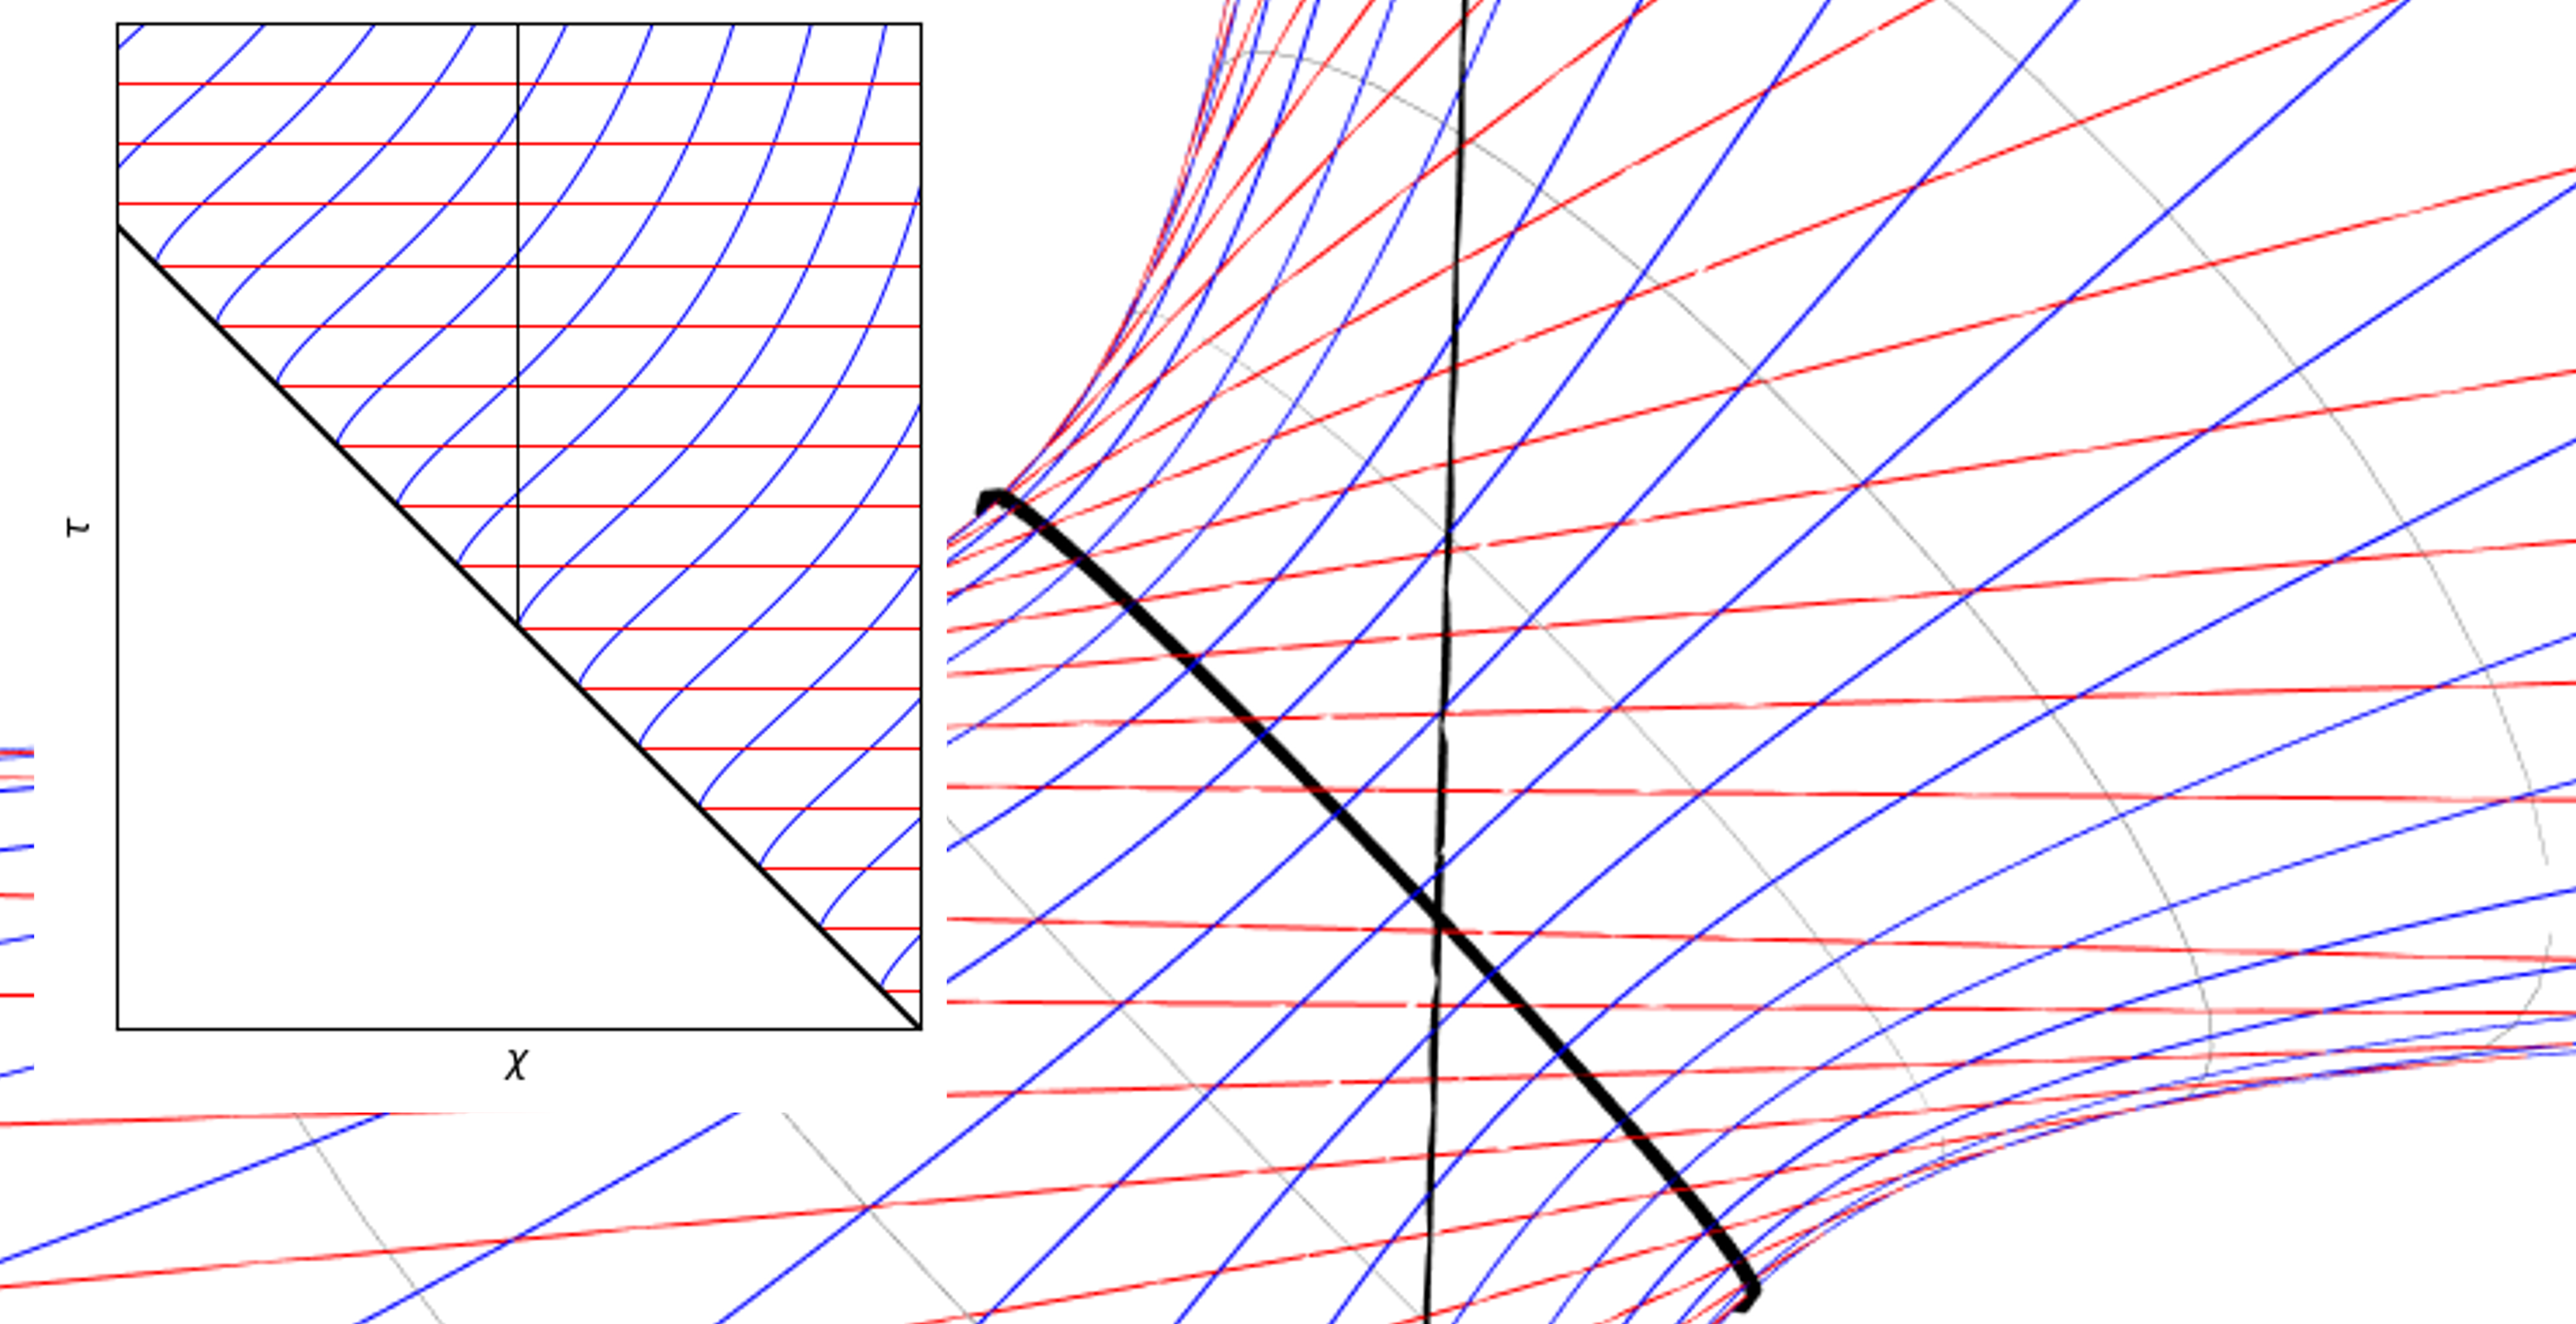
\includegraphics[width=6.5in]{dS-SdS.png}
\caption{A reinterpretation of de~Sitter space within the CR framework. A single fundamental worldline (black) defines the rest frame of real cosmic space, constructed from one bundle of flat null geodesics. The orthogonal red lines represent flat spatial slices at constant proper time, while the evolving 3-sphere foliation is displayed with grey circles along the hyperboloid. The blue worldlines, which are comoving in the standard de~Sitter frame, are reinterpreted as null geodesics (i.e.\ photons) in this causal structure. The inset displays the same construction in proper $(\chi,\tau)$ coordinates, where diagonal lines of constant $\tau+\chi$ define the evolving 3-sphere. This construction alters the causal metric structure without changing the spatial foliation, yielding a non-synchronous cosmological model whose expansion history exactly reproduces that of flat $\Lambda$CDM.}
\label{fig:dS_SdS}
\end{figure*}

This reinterpretation does more than illustrate CR's flexibility---it demonstrates its ability to resolve a foundational philosophical challenge: the hole argument. \logiclink{L5.50}{} In standard GR, different metric assignments inside a fixed boundary can represent mathematically distinct but empirically equivalent universes, leading to worries about indeterminacy. But CR avoids this dilemma by identifying the real universe as projected onto a fixed foliation---cosmic space evolving over time---while treating space-time, together with its causal structure, as a derived, phenomenal representation. The redefinition here shows precisely how two diffeomorphically related metrics can describe the same underlying reality when the ontological commitments are made explicit. The ``hole'' is not a gap in being, but a freedom in representation.

This reinterpretation exemplifies CR's core conceptual move: rather than treating space-time geometry as an ontological given, CR identifies the real universe as projected onto a specific foliation---in this case, the expanding three-sphere---while allowing causal structure to be derived separately. The fact that this reinterpretation preserves diffeomorphism invariance while radically altering the causal metric underscores the layered nature of CR. In this sense, CR completes the project that relationalist interpretations left unfinished. It does not merely assert that physical meaning arises from structure---it identifies which structure. The foliation is not just a computational convenience or a dynamical choice; it is the scaffold of cosmic reality.

To construct a space-time that respects both this new causal structure and the cosmic foliation, we introduce a key change: we treat the radius of the expanding 3-sphere as a timelike coordinate $r$. Since the cosmic 3-sphere is always orthogonal to this timelike direction, the spatial structure in the two dimensions where fundamental observers are at rest should remain unchanged, described by spherically symmetric coordinates about comoving observers. Therefore, a general line-element satisfying these conditions can be written as:
\begin{equation}
    ds^2=-B(r,t)dr^2+A(r,t)dt^2+r^2d\Omega^2,\label{eq:JB}
\end{equation}
where $d\Omega^2$ describes the two spherically symmetric spatial dimensions that contract and expand with $r$, the universe's radius and timelike coordinate.

This redefined structure must still satisfy the vacuum Einstein equations with a positive cosmological constant, as it fundamentally describes a variation of dS space. Solving these equations constrains the functions $B(r,t)$ and $A(r,t)$, yielding the Schwarzschild-de Sitter (SdS) metric:
\begin{equation}
    \mathrm{d}s^2=-\frac{r}{\frac{\Lambda}{3}r^3+\frac{2GM}{c^2}-r}\mathrm{d}r^2+\frac{\frac{\Lambda}{3}r^3+\frac{2GM}{c^2}-r}{r}\mathrm{d}t^2+r^2\mathrm{d}\Omega^2,\label{eq:SdS_statical}
\end{equation}
which is a valid cosmological model for $r>0$ as timelike when the inequality
\begin{equation}
    \frac{\Lambda G^2 M^2}{c^4} > \frac{1}{9}
\end{equation}
is satisfied. This constraint imposes a minimum total mass necessary for the SdS solution to describe a cosmological model, requiring:
\begin{equation}
M > \frac{c^2}{3\sqrt{\Lambda G}} \approx 4.3 \times 10^{52}~\text{kg}.
\end{equation}
By comparison, the calculated baryonic mass of our observable universe, $M_{b,\text{horizon},0} = 1.5 \times 10^{53}~\text{kg}$, and the total mass including dark matter, $M_{m,\text{horizon},0} = 9.6 \times 10^{53}~\text{kg}$, both exceed this threshold. This confirms that the SdS model is consistent with known mass-energy constraints, providing a novel geometric perspective on the total mass distribution of the universe.

The coordinate singularity at $r=0$ in Eq.~(\ref{eq:SdS_statical}) does not correspond to a physical singularity but arises as a consequence of the causal redefinition. Unlike curvature singularities, such as the Schwarzschild singularity at $r=0$, this feature is an artefact of the coordinate system. The original dS space-time contains no singularities, and the introduction of $r$ as a timelike coordinate in SdS merely relocates the degeneracy of the coordinate system. This is analogous to how Schwarzschild coordinates become degenerate at the Schwarzschild horizon, even though the space-time is regular there.

This implies that the singularity does not represent a breakdown of the theory but rather marks the limit of the new coordinate system. Just as Schwarzschild coordinates break down at $r_{\mathrm{Sch}}$ but are extended by Eddington-Finkelstein coordinates, the coordinate singularity at $r=0$ could, in principle, be reformulated in an alternative coordinate system. However, because the foliation of cosmic time remains well-defined in the SdS formulation, no additional extension is necessary for the cosmological interpretation.

In fact, this entire construction enacts CR's formal resolution of the hole argument in practice. \logiclink{L5.51}{} The coordinate redefinition shifts which geodesics are considered null and which are timelike, transforming the metric structure while preserving the underlying spatial evolution. This shows that the indeterminacy feared in standard GR arises only when we fail to distinguish between coordinate identity and real physical structure. Once we recognise that cosmic evolution is defined by the foliation, not the metric field assignments, the apparent ambiguity vanishes. The SdS model and its standard dS counterpart are not rival universes, but two phenomenal maps of the same ontological territory. CR thus not only resolves the hole argument in principle---it enacts its dissolution in practice. The SdS model does not sidestep the paradox; it absorbs and resolves it through ontological clarity.

A key question that arises in this cosmological model is how an anisotropic space-time geometry can still lead to an isotropic observational universe. The resolution lies in the fact that \logiclink{L5.46}{} the fundamental observers are comoving within a maximally symmetric space and that the speed of light is invariant.

First, while the slices of constant cosmic time $r$ are not isotropic and homogeneous in this frame, this results from the nontrivial evolution of fundamental observers along their geodesics rather than from an intrinsic inhomogeneity of space. By construction, space itself remains maximally symmetric as an expanding 3-sphere. The anisotropy is therefore a feature of the coordinate description rather than of the fundamental spatial structure.

Second, the comoving fundamental observers do not experience relative motion apart from cosmic expansion. Because light propagates along null geodesics, its speed must remain the same in all directions relative to these observers. This follows directly from the invariance of the speed of light: in any local frame, photons travel at $c$ in all directions, just as in special relativity. Consequently, fundamental observers necessarily perceive an isotropic universe, as all incoming light reaches them in an isotropic manner.

To understand the observational implications of this cosmological model, we examine the proper reference frame of fundamental observers. These observers correspond to the bundle of geodesics that remain at rest with respect to the vanishing of the gravitational potential in the metric. Their speed through $t$ over the course of $r$ is purely a consequence of the underlying geometry. The line-element in this coordinate frame is \cite{Janzen2015}:
\begin{equation}
    ds^2=-d\tau^2+(\partial_{\chi}r)^2d\chi^2+r^2d\Omega^2,\label{eq:SdS_flat}
\end{equation}
where
\begin{equation}
    r(\tau,\chi)=\left(\frac{6GM}{\Lambda c^2}\right)^{1/3}\sinh^{2/3}\left(\frac{3}{2}\sqrt{\frac{\Lambda}{3}}[\tau+\chi]\right),\label{eq:r_SdS}
\end{equation}
defined on the interval $\tau+\chi>0$.

This line-element exhibits several striking features. First, $r$ does not evolve with the proper time $\tau$ of any particular fundamental worldline, but with the parameter $c\tilde{\tau}\equiv\tau+\chi$, which is tilted with respect to the fundamental rest frame. That is, \textit{this universe is not synchronous in the fundamental rest frame}---a direct consequence of the causal redefinition.

Furthermore, while slices of constant $\tau$ are Euclidean (since $\partial_{\chi}rd\chi=dr$), these are not cosmological spatial slices. The lines perpendicular to the $\tau$-direction correspond to the complementary bundle of null geodesics, which are perpendicular at the ``throat'' of the de~Sitter hyperboloid to the bundle of worldlines defining fundamental observers (see Figure~\ref{fig:dS_SdS}). These orthogonal lines form a complementary reference frame, extending from a finite distance at $\chi=-\tau$ to $\chi=+\infty$, with synchronous events spanning cosmic time from $r=0$ out to $r\rightarrow\infty$. 

A second remarkable feature of this line-element is that $r(\tilde{\tau})$ is \textit{identical} to the scale factor of the flat $\Lambda$CDM model:
\begin{equation} 
    \frac{a(\tilde{\tau})}{a_0}=\left(\frac{3H_0^2\Omega_{m,0}}{\Lambda c^2}\right)^{1/3}\sinh^{2/3}\left(\frac{3}{2}\sqrt{\frac{\Lambda c^2}{3}}\tilde{\tau}\right).\label{eq:scalefac} 
\end{equation} 
This is an astonishing result: \logiclink{L5.45}{} \logiclink{L5.47}{} the expansion history of \textit{this} universe, when described in the proper rest frame of the reinterpreted null geodesics, follows \textit{exactly} the phenomenological expansion rate of the flat $\Lambda$CDM model, the standard model of cosmology that has been constrained through FLRW model-fitting \citep{Aghanim2020}. In other words, an observer in this universe would see the same redshift-distance relation, the same relic radiation history, and the same apparent flow of cosmic time---even though the underlying structure is neither synchronous nor driven by energy content. This is, in fact, an astonishing coincidence. This model makes no dynamical assumptions about energy density or synchrony, yet recovers the exact expansion history of flat $\Lambda$CDM. This striking alignment strongly suggests that the observed coherence of cosmological expansion may arise from geometric structure alone, rather than from energy-driven dynamics. Whether this alignment reflects a deeper geometric necessity or an empirical fluke remains an open question.

This reinterpretation also leads to a testable prediction. The standard flat $\Lambda$CDM model assumes a noumenally flat universe whose expansion history is dynamically determined by its energy content. Crucially, in the early universe, radiation density plays a dominant role in setting the expansion rate, significantly shaping the acoustic scale and the resulting CMB anisotropy spectrum. In the standard model, this early coupling is not optional---it is a structural necessity of the Einstein field equations when applied to a synchronous, energy-driven foliation. But in the CR/SdS model, this coupling is absent at the ontological level: the expansion is governed by geometric structure, not by energy content. Radiation has no influence on the expansion rate in early cosmic time because the expansion does not depend on stress-energy, but on the layered projection of an evolving 3-sphere. \logiclink{L5.52}{} This divergence has observational consequences and may be testable in principle. However, any such analysis must proceed carefully: one would need to model the evolution of the sound horizon within the noumenal geometry of the 3-sphere, then rigorously translate that structure through the projection process into the phenomenal space-time frame where observational data are interpreted. While this book does not perform that modelling, it establishes the theoretical framework necessary to derive such predictions and sets the stage for empirical evaluation.

\logiclink{L5.48}{} This identity is more than just a mathematical coincidence: it suggests that the standard FLRW phenomenology, typically assumed to require a synchronous space-time structure, may instead emerge naturally from the causal structure redefinition applied within this cosmological model. Rather than requiring matter-energy content to dictate the universe's evolution, the SdS framework inherently enforces a uniform expansion history, with the same observational consequences as a flat $\Lambda$CDM universe.

This final example drives home the core insight of CR. By rejecting the assumption that space-time is identical with reality, and by embracing a layered ontology where space evolves independently of causal structure, CR reveals how many of relativity's conceptual puzzles can be resolved without modifying its dynamical laws. The observed expansion of the universe is not an illusion---but neither is it the literal stretching of space-time. It is, rather, \logiclink{L5.49}{} the evolving projection of a deeper structure: real, three-dimensional space expanding in the course of absolute cosmic time. The layered geometry of Cosmological Relativity transforms expansion from a postulate into a consequence---restoring coherence to the largest scale of all. In the next section, we lay out how this framework should now be applied in practice, and what interpretive shifts it demands from the foundations of physics.

\section[Interpreting Space-Time Ontology in CR]{Interpreting Space-Time Ontology in Cosmological Relativity}\label{sec:5.5}
\noindent\textit{Supports Logic Map B nodes: \hyperref[appendix:III4]{[III4]}, \hyperref[appendix:IV1]{[IV1]}, \hyperref[appendix:IV2]{[IV2]}, \hyperref[appendix:IV3]{[IV3]}, \hyperref[appendix:IV4]{[IV4]}, \hyperref[appendix:IV5]{[IV5]}, \hyperref[appendix:V1]{[V1]}, \hyperref[appendix:V2]{[V2]}, \hyperref[appendix:V3]{[V3]}, \hyperref[appendix:V4]{[V4]}, \hyperref[appendix:V5]{[V5]}.}

\vspace{4pt}

We may now complete the progression established in Chapters~\ref{sec:3} and~\ref{sec:4}. In Chapter~\ref{sec:3}, we showed that interpreting the space-time block as ontologically real requires smuggling in a fifth dimension of meta-time, undermining its own metaphysical premise. The block universe is not timeless---it merely displaces the flow of time one level up. In Chapter~\ref{sec:4}, we saw that operational relativism, in denying the existence of noumenal structure, collapses into selective realism: it ends up invoking precisely the structures it claims to reject. By refusing to distinguish between appearances and reality, it becomes conceptually incoherent.

CR resolves these contradictions by restoring a coherent ontology of space and time. It does not simply reject previous frameworks---it clarifies why they failed, what they overlooked, and how their descriptive successes can be retained within a more principled metaphysical foundation.

The core insight is this: \logiclink{L5.53}{} space-time is not reality. It is a derived, phenomenological record of the evolving structure of the universe. The real cosmos is not a four-dimensional block, nor an observer's past light cone, but a three-dimensional spatial entity that exists and evolves in absolute cosmic time. \logiclink{L5.59}{} Events do not exist ``in'' space-time. They happen in space, and space-time records their becoming. The manifold is not an arena in which reality unfolds; it is the trace of an existing universe.

This distinction is not philosophical indulgence---it is a structural necessity. Without it, relativistic physics collapses into paradox. The block universe cannot explain the experience of becoming without smuggling in flow; operationalism cannot model the universe without smuggling in simultaneity. Both end up violating their own principles. CR avoids these contradictions because it never denies the empirical phenomena that these frameworks try to explain away. It accounts for them. \logiclink{L5.54}{} \logiclink{L5.57}{} Flow, simultaneity, and temporal order all arise naturally from CR's layered geometry. They are not illusions. They are the structural expressions of a cosmos that truly evolves.

In this way, CR recovers the power of general relativity without succumbing to its interpretive instabilities. It affirms the full empirical content of GR's formalism while grounding that formalism in an ontology that distinguishes between what exists and what is measured, between what is structurally real and what is relationally described. By treating space-time as a record rather than a substance, CR resolves the metaphysical overreach that has long plagued relativistic interpretation.

It does not claim that GR failed as a physical theory, only that its success has been overinterpreted. CR shows that the manifold is not the world itself, but the shadow it leaves behind---a record of becoming, not the substance that becomes. Observational covariance describes the invariance of that shadow---but CR restores the structure that casts it. Covariance ensures that all observers agree on empirical predictions; it does not require that reality itself be a structureless manifold. CR clarifies that while observations must be frame-independent, ontological structure need not be. GR describes the record of becoming; CR restores becoming itself.

This does not make CR a rejection of relativity. Quite the opposite. It preserves the full empirical success of both special and general relativity while correcting their conceptual misreadings. CR accepts the relativity of simultaneity as a feature of observational appearance, not of underlying structure, and retains full relativistic covariance for all empirical predictions. In this sense, CR stands to operational relativism and the block universe as Copernicus stood to Ptolemy: not as a rejection of observational accuracy, but as a principled reinterpretation that reveals the deeper structure behind the appearances.

This reinterpretation also recasts the ontological status of gravitational singularities. In standard GR, the Big Bang and black hole interiors are treated as physical points where the manifold---and often the laws of physics themselves---break down. CR reframes this entirely. These so-called ``singularities'' are not necessarily ontological objects or literal locations in space-time; they are \textit{representational boundaries}---places where the projection of an evolving spatial reality into a four-dimensional record ceases to be well-behaved \logiclink{L5.60}{}. Like vanishing points in a perspective drawing, they may reflect the limits of the projection, not necessarily the limits of reality itself. This may apply even to so-called coordinate singularities: while mathematically removable, they can mark regions where the projection loses ontological reference---like extending radius values below zero in a polar map. The singularity is not necessarily ``in'' the universe; it may instead mark the outer edge of what the space-time manifold can encode. In this view, singularities are not necessarily physically catastrophic---they are, at least in part, artefacts of representational geometry.

What appears as a breakdown in GR is, in CR, a boundary beyond which the projection loses contact with the underlying ontology---not because the structure fails, but because it is no longer expressible within the space-time formalism. CR thus preserves ontological coherence where standard interpretations predict incompleteness, reframing the problem of singularities as a feature of the projection rather than of physical law.

This also reframes the role of diffeomorphism invariance. In standard GR, the requirement that physical predictions be invariant under smooth coordinate transformations is often taken to imply a radical form of ontological indifference---as if nothing exists beyond the relational structure of fields on a manifold. \logiclink{L5.55}{} CR retains full diffeomorphism invariance, but reframes its domain: invariance applies to the space-time record, not to the evolving universe itself. The real structure of the cosmos is not defined by the manifold; it underlies and constrains the manifold's content. Coordinates describe appearances. The layered geometric framework of CR describes being. This layered geometric framework---where space is a real, evolving three-dimensional structure, time is an absolute parameter of becoming, and space-time is a record projected from these---is what distinguishes CR from traditional GR.

In short, CR provides the missing ontological architecture. It distinguishes noumena from phenomena without invoking metaphysical excess. It recovers flow without smuggling it in. It defines simultaneity without privileging synchrony. It reconciles relativity's descriptive power with a coherent account of what exists. And it explains---for the first time---why space-time appears the way it does, without mistaking that appearance for the thing itself.

This insight echoes Eddington's own suspicion that cosmological structure must reflect an underlying geometrical order \citep{Eddington1923}. CR formalises that suspicion, showing that the universe's expanding, isotropic appearance is not a projection onto empty space-time, but a reflection of the layered evolution of real, three-dimensional space.

Throughout this book, we have developed a precise logical framework to expose the structural failures of rival interpretations. CR is not a speculative alternative---it is the only model that meets the logical and empirical constraints established across all preceding chapters. This is not merely a reinterpretation of GR. \logiclink{L5.56}{} It is a structural augmentation. CR fills in the topological and geometric gaps that the standard theory left open, not by altering its equations, but by specifying the ontological commitments necessary to interpret them coherently. In doing so, it transforms the interpretation of relativistic physics from a domain of paradox into a field of clarity. \logiclink{L5.58}{} The conceptual errors of the twentieth century are not to be dismissed, but understood. They arose not from mathematical failure, but from a refusal to distinguish the map from the territory. The failure of previous interpretations is not merely conceptual---it is modal: they assert what must be true in all frames while denying the ontological structure that could make such claims coherent.

To be clear: the contradictions identified in earlier chapters are not merely loosened by CR---they are resolved. The smuggled meta-time of the block universe becomes unnecessary once becoming is restored as a structural feature of reality. The ambiguous ontology of Operational Relativism collapses when noumena are distinguished from phenomena and given real structure. The paradoxes of black hole formation, simultaneity, causal asymmetry, and event individuation dissolve once the layered geometry of CR is applied consistently. Singularities are no longer treated as ontological endpoints, but as projective artefacts---limits of representation, not of existence. In each case, the conceptual tension is not papered over---it is reinterpreted and resolved at its root. CR does not merely offer a new ontology. It offers the only ontology that allows relativistic physics to describe a world that changes, explains, and exists without contradiction.

Cosmological Relativity explains what the territory is, distinguishing it from the map. This is the natural next step in the tradition of Einstein, Weyl, and Eddington---not a repudiation of their insights, but the completion of a project they began but could not yet finish. It hands back the territory---and with it, the structural clarity relativistic physics has long lacked.

\chapter{Restoring the Territory}\label{sec:6}
\noindent\textit{Supports Logic Map B nodes: \hyperref[appendix:IV5]{[IV5]}, \hyperref[appendix:V3]{[V3]}, \hyperref[appendix:V4]{[V4]}, \hyperref[appendix:V5]{[V5]}.}

\vspace{4pt}

This book has traced a deep and underacknowledged failure in modern interpretations of relativistic physics. The dominant frameworks---Block Universe eternalism and Operational Relativism---each attempt to address the ambiguity, incoherence, and apparent flow of relativistic time by denying one of its structural features. But in each case, the result is not clarity, but contradiction. The Block Universe denies temporal flow while covertly relying on a meta-time that allows it to speak of what \textit{exists}. Operationalism denies simultaneity while making selective ontological commitments that require it in practice.

\textit{\logiclink{L6.2}{} Physics today is not confused because of bad models---it's confused because it makes metaphysical commitments without admitting them, then refuses to clean up the mess when contradictions arise.}

This is not simply the failure of two interpretations. It is the failure of an entire strategy: the belief that one can interpret without committing. The attempt to describe space-time while bracketing ontology does not lead to caution---it leads to collapse. Neutrality, when it conceals metaphysical structure, becomes evasion. A science that cannot articulate what its models commit to cannot explain what those models mean. The Block Universe, in turn, does not merely overcommit---it self-destructs. It invokes existence while denying flow, but cannot express that existence without implicitly importing a meta-time. Its supposed neutrality masks a deep incoherence: the need to reintroduce what it pretends to deny. Without acknowledging becoming, it cannot explain the appearance of time at all.

Cosmological Relativity offers a principled way out. It accepts the empirical framework of relativity, including general covariance and diffeomorphism invariance. But it formally augments this framework with a layered geometric ontology in which space-time is fundamentally reinterpreted as a projection from real, evolving structure---a record of events in a three-dimensional cosmos governed by absolute cosmic time.

This is not just a reframing of familiar tools. It is a structural extension that fills in what GR left unstated: the ontological scaffolding required to make sense of the very phenomena it describes.

The layered framework of CR resolves the contradictions diagnosed throughout the book---those of metaphysical overreach in eternalism, of selective realism in operationalism, and of linguistic and conceptual collapse in the standard ontology of space-time.

This move restores clarity to longstanding paradoxes. Gravitational collapse no longer requires event horizons to form in finite time. Time travel becomes not paradoxical, but meaningless. Singularities are no longer catastrophic breakdowns, but representational boundaries. The hole argument becomes a misdiagnosed conflation of mathematical symmetry and ontological identity. And cosmic expansion---far from being a puzzling dynamical effect we can \textit{describe}, but which lacks a fundamental \textit{explanation}---emerges naturally from the causal geometry of an evolving universe, as clarified by the reinterpretation of de~Sitter geometry in \S~\ref{sec:5.4.6}.

CR does not deny the phenomena that have shaped relativistic physics. It explains them. And in doing so, it dissolves the artificial dichotomies---between past and future, observer and reality, time and structure---that have long hindered a coherent account of relativistic becoming and causal structure.

The result is not just a new interpretation. It is a restored ontology. Time flows. Reality evolves. And experience reflects the real structure of the world. The conceptual and empirical conclusions reached here are not speculative assertions. They follow from a precise chain of logical inferences, each developed and supported in detail across the structure of the book. 

\logiclink{L6.3}{} In this light, CR marks more than a technical or philosophical refinement---it signals a moment of scientific maturity. A science that refuses to distinguish between appearance and structure, or that collapses its own commitments into operational prescriptions, is not an honest science. It is a method performed by rote, hoping its paradoxes will resolve themselves through silence. \logiclink{L6.4}{} The lesson of CR is that explanatory discipline must take precedence over ideological comfort. \logiclink{L6.1}{} Space-time is not reality; it is the record of reality. When physics restores the distinction---it restores its soul. 

\appendix

\chapter[Rewiring the Language of Eternalism]{Rewiring Eternalism: A Linguistic Correction of Greene's (2004) ``The Frozen River''}\label{sec:appendix:greene}

The following is a reconstructed version of Brian Greene's widely cited presentation of the Block Universe, drawn from \textit{The Fabric of the Cosmos} (2004, Chapter 5: ``The Frozen River''). This revision replaces existential verbs with non-existential copulas to expose and eliminate tacit metaphysical commitments. The aim is not to critique Greene as an expositor, but to use his lucid summary to demonstrate how Eternalist rhetoric routinely relies on grammatical structures it cannot ontologically defend.

Following the linguistic framework developed in \S~\ref{sec:3.4}, we apply two analytic tools: the non-existential copulas \textit{iz} and \textit{zare}, which replace the existentially loaded copulas `is' and `are' when applied to a-temporal objects, and a tiered asterisk notation. A single asterisk (*) flags terms that inherently apply to temporally persisting objects, whether changing or permanent, which can be safely rendered as terms ``on holiday'' via explicit non-existential flagging; a double asterisk (**) marks terms that explicitly assert metaphysical endurance or existence, loading non-trivial ontological commitment that renders claims structurally incompatible with pure 4D Eternalism.

Perceptual verbs are marked only when used to describe experiences \textit{within} the Block that imply cognitive continuity or diachronic identity across slices---cases that structurally presuppose meta-endurance, persistence, or permanence of space-time, thereby temporally loading the concept. In such cases, the above framework is applied. In contrast, phenomenological descriptions made \textit{from outside} the Block, or referring to generalised human experience, are unmarked, but potentially footnoted if they are structurally misleading.

Footnotes are added where word-level substitutions cannot resolve ontological contradiction. These highlight formulations that depend on tacit metaphysical scaffolding and clarify where Eternalism collapses into incoherence under its own grammatical weight.\\
\vspace{0.1pt}\hrulefill\\

So: \textit{if you buy the notion that reality consists* of the things in your freeze-frame mental image right now*, and if you agree that your} now \textit{iz no more valid than the} now \textit{of someone located far away in space who can move* freely, then reality encompasses** all of the events in spacetime.} The total loaf exists**. Just as we envision* all of space as \textit{really} being* out there,\footnote{Technically, this clause is structurally misleading. The way we envision space as really being out there is in an enduring manner, not as an instantaneous state. To say that all of time should be thought of as really being out there in the way we envision all of space as being out there surreptitiously injects a meta-temporal framework, implying that all events are equally ``present'' in an extended sense that mirrors spatial co-presence, which contradicts the very denial of temporal passage. A more accurate analogy would be to compare all of time to the way we envision the events that happen throughout space at a particular instant.} as \textit{really} existing*, we should also envision all of time as \textit{really} being** out there, as \textit{really} existing**, too. Past, present, and future certainly appear to be distinct entities, but as Einstein once said, ``For we convinced physicists the distinction between past, present, and future is only an illusion, however persistent.'' The only thing that iz real iz the whole of spacetime.

In this way of thinking, events, regardless of when they happen from any particular perspective, just \textit{are}**. They all exist**. They eternally** occupy* their particular point in spacetime. There iz no flow. If you were having a great time at the stroke of midnight on New Year's Eve, 1999, you still** are**, since that iz just one immutable** location in spacetime. It is tough to accept this description since our worldview so forcefully distinguishes between past, present, and future. But if we stare intently at this familiar temporal scheme and confront it with the cold hard facts of modern physics, its only place of refuge seems to lie within the human mind.

Undeniably, our conscious experience seems to sweep through the slices.\footnote{This paragraph highlights an important distinction. Sentences like ``our conscious experience seems to sweep through slices,'' which convey a \textit{perception} of real existence, are not categorically invalid. Nor are statements attributing such perception to inhabitants* within a block universe---though such descriptions are conceptually misleading and therefore problematic. However, characterisations of the block universe or of events as ontologically existing or enduring are not just misleading but structurally invalid. Likewise, statements that imply such inhabitants* persist in meta-time cross from metaphor into contradiction. As our aim here is to minimally edit the excerpt---correcting invalid formulations and annotating structurally misleading ones---clauses like the opening sentence, which are technically valid but heuristically dangerous, have been left intact. Nonetheless, such constructions should ideally be avoided or used with clear qualification.} It is as though our minds provide the projector light referred to earlier, so that moments of time come to life when they are illuminated by the power of consciousness. The flowing sensation from one moment to the next arises from our conscious recognition of change in our thoughts, feelings, and perceptions, and the sequence of change seems to have a continuous motion; it seems to unfold* into a coherent story. But---without any pretense of psychological or neurobiological precision---we can envision how we might experience* a flow* of time even though, in actuality, there may be* no such thing. To see what I mean, imagine playing \textit{Gone with the Wind} through a faulty DVD player that randomly jumps forward and backward. One still frame flashes momentarily on the screen and is followed immediately by another from a completely different part of the film. When you watch this jumbled version, it will be hard for you to make sense of what's going on. But Scarlett and Rhett have* no problem. In each frame, they do* what they have* always** done* in that frame.\footnote{In this sentence, nearly every verb implies persistence or meta-endurance. While most can be read `on holiday,' the accumulation builds toward an ontological reading that Eternalism cannot support.} Were you able to stop the DVD on some particular frame and ask* them about their thoughts and memories, they'd respond* with the same answers they would have** given** had you played the DVD in a properly functioning player. If you asked* them whether it was* confusing* to romp around* through the Civil War out of order*, they'd look* at you quizzically and figure* you had* tossed* back one too many mint juleps. In any given frame, they'd have* the thoughts and memories they have* always** had* in that frame. And in particular, those thoughts and memories would give* them the sensation that time iz smoothly* and coherently* flowing* as usual.

Similarly, each moment in spacetime---each time-slice---iz like one of the still frames in a film. It exists** whether or not some light illuminates* it. As for Scarlett and Rhett, to the you who iz in any such moment, it \textit{iz} the \textit{now}, it \textit{iz} the moment you experience* at \textit{that} moment. And it always** will be**. Moreover, within each individual slice, your thoughts and memories zare sufficiently rich to yield* a sense that time has* continuously* flowed* to that moment. This feeling*, this sensation* that time iz flowing*, doesn't require* previous moments---previous frames---to be* ``sequentially illuminated*.''\footnote{This sentence is linguistically structured as a phenomenological report, but it assigns perceptual and cognitive continuity to entities presumed to exist within the Block. That attribution is structurally incoherent. A feeling or sensation of temporal flow cannot be coherently located in a single slice without presupposing memory or diachronic awareness, which require meta-time---precisely what the Block Universe denies. The contradiction is not merely semantic but ontological: an existential experience cannot be embedded within a non-existential ontology.}

\vspace{1em}
\noindent
[\textit{The following paragraph, unlike earlier ones, cannot be coherently annotated. Its metaphysical presuppositions are not merely misworded but internally contradictory. It presents a false dilemma---between events as objects that may either \textit{change} or merely \textit{exist} eternally---that arises only if one assumes, incorrectly, that events ``exist'' in the first place. But events do not exist; they simply happen. They do not persist and therefore categorically cannot change. The very assignment of ``being''---whether to events, to moments that cut across space, or to all of space-time---is a category error. It reintroduces meta-time through the notion of ontological permanence, which is itself fundamentally loaded, as that very \textit{permanence} tacitly supposes non-trivial temporality. And since both sides of the dilemma presented here presuppose this sense of existence, altering the text by replacing offending terms with non-existential counterparts would render the entire paragraph incoherent. Therefore, we present it unmodified, not as a candidate for repair, but as an exhibit of irreducible confusion.}]
\vspace{1em}

And if you think about it for a moment, you'll realise that's a very good thing, because the notion of a projector light sequentially bringing moments to life is highly problematic for another, even more basic reason. If the projector light properly did its job and illuminated a given moment---say, the stroke of midnight, New Year's Eve, 1999---what would it mean for that moment to then go dark? If the moment were lit, then being illuminated would be a feature of the moment, a feature as everlasting and unchanging as everything else happening in that moment. To experience illumination---to be ``alive,'' to be the present, to be \textit{the now}---and then to experience darkness---to be ``dormant,'' to be the past, to be what was---is to experience change. But the concept of change has no meaning with respect to a single moment in time. The change would have to occur through time. The change would mark the passing of time. But what notion of time could that possibly be? By definition, moments \textit{don't} include the passing of time---at least not the time we're aware of---because moments just are;\footnote{Up to this point, Greene comes close to articulating the correct category distinction. But here, in this clause, he collapses it. ``Because moments just \textit{are}'' reintroduces the very category error he had just appeared to disavow with ``By definition, moments \textit{don't} include the passing of time.''} they are the raw material of time; they \textit{don't} change. A particular moment can no more change in time than a particular location can move in space: if the location were to move, it would be a different location in space; if a moment in time were to change, it would be a different moment in time. The intuitive image of a projector light that brings each new \textit{now} to life just doesn't hold up to careful examination. Instead, every moment is illuminated and every moment remains illuminated.\footnote{Here is the clearest expression of the false dilemma identified above: the claim that moments cannot change, and therefore must simply \textit{be}---permanently illuminated, unchanging, and enduring, like a block of ice frozen forever. The strongest expression of this fallacy appears in the word \textit{remains}, which explicitly loads meta-time into the claim, clarifying that temporal persistence is not merely implicitly conferred through the copula `is' illuminated, but that the illumination explicitly `remains'. As this book explains, neither horn of this dilemma is valid, because both rest on the same category error. Moments do not exist and thus cannot change. They \textit{happen}; they \textit{are} not; they \textit{zare}. To describe them as objects that ``are'' is to take ``existence'' on holiday.} Every moment \textit{is}. Under close scrutiny, the flowing river of time more closely resembles a giant block of ice with every moment forever frozen into place.

This conception of time is significantly different from what most of us have internalised. Even though it emerged from his own insights, Einstein was not hardened to the difficulty of fully absorbing such a profound change in perspective. Rudolf Carnap recounts a wonderful conversation he had with Einstein on this subject: ``Einstein said the problem of the now worried him seriously. He explained that the experience of the now means something special for man, something essentially different from the past and the future, but that this important difference does not and cannot occur within physics. That this experience cannot be grasped by science seemed to him a matter of painful but inevitable resignation.''

This resignation leaves open a pivotal question: Is science unable to grasp a fundamental quality of time that the human mind embraces as readily as the lungs take in air? Or does the human mind impose on time a quality of its own making, one that is artificial and that hence does not show up in the laws of physics? If you were to ask me this question during the working day, I'd side with the latter perspective. But by nightfall, when critical thought eases into the ordinary routines of life, it's hard to maintain full resistance to the former viewpoint. Time is a subtle subject and we are far from understanding it fully. It is possible that some insightful person will one day devise a new way of looking at time and reveal a bona fide physical foundation for a time that flows. Then again, the discussion above, based on logic and relativity, may turn out to be the full story. Certainly though, the feeling that time flows is deeply ingrained in our experience and thoroughly pervades our thinking and language. So much so that we have lapsed, and will continue to lapse, into habitual, colloquial descriptions that refer to a flowing time. But don't confuse language with reality. Human language is far better at capturing human experience than at expressing deep physical laws.\\
\vspace{0.1pt}\hrulefill

\noindent\textit{Greene concludes with a tension he cannot resolve: the feeling that time flows is so deeply embedded in human experience that it shapes our language, yet it finds no place in physics. But this is not merely a linguistic gap or an epistemic limitation. As this appendix has shown, it reflects a deeper ontological confusion. The Block Universe, as typically described, cannot be coherently expressed without invoking the very flow it denies. Attempts to preserve its structure by reinterpreting ``being'' as permanence or ``illumination'' as timeless presence only reintroduce meta-time by another name.}

\textit{This is not a failure of Greene's intellectual clarity---on the contrary, it is precisely his clarity that exposes the structural inadequacy of the framework itself. The contradiction lies not with the expositor, but with the concept: Eternalism cannot be stated in ordinary language without collapsing into covert flow. The solution is not to force physics to accommodate time's passage, nor to explain it away, but to recognise that the debate has been structured around a false category---one that confuses \textit{what is} with \textit{what happens}, and in doing so, mistakes grammatical error for ontological necessity.}

\chapter{Logic Map: Bottom-Up Inference Structure}
\label{appendix:logicmap-bottomup}

This appendix presents the fine-grained inferential structure of the book's argument. Each entry records a distinct logical inference made in the main text, specifying the type of reasoning (e.g.\ deductive, reductive, analogical), the section(s) in which it appears, its epistemic role, and its logical dependencies. All entries are anchored with labels and hyperlinked to the relevant claims in the body.

To prevent precisely the kind of ontological conflation this book critiques, the argument's full structure is transparently documented in a dual mapping system.

The purpose of this Logic Map is threefold:
\begin{enumerate}
  \item To make the internal coherence of the argument fully transparent and open to scrutiny;
  \item To guide interdisciplinary readers across physics, metaphysics, epistemology, and philosophy of language;
  \item To model a new standard of inspectable, collaborative academic authorship in the era of AI-assisted research.
\end{enumerate}

While no formal proof system is assumed, the structure draws inspiration from a range of existing models, including:
\begin{itemize}
  \item \textit{Argument maps} in analytic philosophy (e.g.\ \cite{harrell2011});
  \item \textit{Semantic networks} and \textit{concept maps} in cognitive science and education (e.g.\ \cite{novak1998learning});
  \item \textit{Dependency graphs} and \textit{belief networks} in AI and probabilistic reasoning (e.g.\ \cite{pearl1988});
  \item \textit{Ontological scaffolding} in formal metaphysics (e.g.\ \cite{smith1998}).
\end{itemize}

However, this framework is distinct in its integration of:
\begin{itemize}
  \item Cross-disciplinary logical types (deductive, inductive, reductive, constructive);
  \item Epistemological awareness of how scientific inference functions across disciplines;
  \item Precise textual anchoring to an argumentative manuscript, allowing for direct auditability;
  \item A collaborative human–AI authorship context.
\end{itemize}

This is not a tool for formalisation per se, but for epistemic clarity. It enables readers to trace the logic of every claim and inspect its justification. It offers a transparency model not just for this book, but for interdisciplinary philosophy of science more broadly.

In this way, the Logic Map mirrors the central insight of the book: that no argument should rely on implicit metaphysical commitments or linguistic habits. Appearance must never substitute for structure. What follows is the full inferential skeleton of the argument---laid bare for inspection, critique, and refinement.

\vspace{1em}
\hrule
\vspace{1em}

\subsection*{L1.1: Epistemic Instability of Mixed Ontologies}
\label{appendix:L1.1}
\textbf{Type:} Deductive (Epistemological) \\
\textbf{Sections:} 1.1 \\
\textbf{Claim:} A scientific theory whose formal description implies one ontology while its practical application relies on a different ontology is epistemically unstable and logically incoherent.
\begin{itemize}
  \item The scientific method requires theories to maintain internal logical consistency between descriptive structure and applied usage.
  \item Ontology refers to the structure of reality implicitly or explicitly posited by a theory's formal framework.
  \item If a theory's formal description implies ontology A, but its operational application presupposes ontological structures inconsistent with A (i.e., ontology B), the resulting mismatch constitutes an unresolved contradiction.
  \item Such contradictions compromise the explanatory coherence and conceptual integrity of the theory.
  \item Therefore, the theory is epistemically unstable and cannot serve as a coherent account of physical reality.
\end{itemize}
\textbf{Dependencies:} None \\
\textbf{Notes:} If (a theory implies ontology A but succeeds only by using ontology B) then (epistemic contradiction). Therefore: incoherent. This is a foundational epistemic principle that underlies the central critique of both the Block Universe and Operational Relativism. This does not imply empirical invalidity, but rather a conceptual failure to specify what kind of world the theory purports to describe. Examples of this contradiction are demonstrated throughout Chapters 3, 4, and 5.\\
\returnlink{L1.1}

\subsection*{L2.1: Repetition of Distant Events due to Observer Motion (Incoherence of Now)}\label{appendix:L2.1}
\textbf{Type:} Deductive \\
\textbf{Sections:} 2.4 \\
\textbf{Claim:} An observer moving cyclically relative to a distant system will describe a single distant event as happening repeatedly due to relativistic simultaneity shifts.
\begin{itemize}
  \item The relativity of simultaneity causes time slices to shift depending on an observer's velocity.
  \item Earth's orbital velocity changes cyclically over the year.
  \item The relative velocity to Andromeda therefore oscillates between $+26$ and $-26$ km/s.
  \item This leads to a calculated simultaneity shift of $\pm217$ years.
  \item Over one orbit, we assign \textit{many different times} to the same event in Andromeda.
  \item Therefore, a single distant event is described as occurring \textit{repeatedly} on the same worldline, revealing incoherence in the naive present.
\end{itemize}
\textbf{Dependencies:} None \\
\textbf{Notes:} This is the first formal paradox implied by SR that destabilises naive presentism and motivates the need for an interpretive framework.\\
\returnlink{L2.1}

\subsection*{L2.2: Ambiguity of Simultaneity (One-to-Many)}\label{appendix:L2.2}
\textbf{Type:} Deductive \\
\textbf{Sections:} 2.2 \\
\textbf{Claim:} The relativity of simultaneity implies that one event may be simultaneous with many different distant events, depending on the observer's velocity.
\begin{itemize}
  \item In special relativity, simultaneity is defined in terms of clock synchronisation within inertial frames.
  \item When observers are in relative motion, they assign different distant events to be simultaneous with the same local event.
  \item The aliens' relative velocities produce ±37-hour shifts in what they regard as Earth's ``now.''
  \item Therefore, one single event (the alien high-five) corresponds to \textit{many different} events on Earth being described as simultaneous.
\end{itemize}
\textbf{Dependencies:} None \\
\textbf{Notes:} This inference sets up the idea of simultaneity as frame-relative and ambiguous, laying the groundwork for deeper ontological contradictions.\\
\returnlink{L2.2}

\subsection*{L2.3: Collective Flow and Continuous Flux}\label{appendix:L2.3}
\textbf{Type:} Inductive \\
\textbf{Sections:} 2.3 \\
\textbf{Claim:} The superposition of relativistic reference frames results in an emergent sense of temporal flow across a continuous stretch of Earth's worldline.
\begin{itemize}
  \item Each observer in motion assigns a slightly different simultaneity slice to Earth's events.
  \item These perspectives, taken together, span a wide range---here, 8.4 years centered around Earth's present.
  \item Since each frame observes a \textit{continuous sequence} of Earth's events, this creates an ensemble sense of unfolding.
  \item Therefore, time on Earth appears to ``flow'' not in one direction, but in overlapping slices depending on the observer.
  \item This is not a formal result of SR, but a phenomenological implication of the system's total structure.
\end{itemize}
\textbf{Dependencies:} L2.2 \\
\textbf{Notes:} This inference marks the first emergence of apparent flow---later reframed as a projection arising from observer-relative ontology.\\
\returnlink{L2.3}

\subsection*{L2.4: The Interpretation Gap (Need for Frameworks)}\label{appendix:L2.4}
\textbf{Type:} Reductive \\
\textbf{Sections:} 2.5 \\
\textbf{Claim:} The formalism of relativity theory underdetermines its ontological interpretation, necessitating external conceptual frameworks.
\begin{itemize}
  \item Relativity provides precise mathematical predictions.
  \item It defines simultaneity, time dilation, and length contraction via formal operations on space-time.
  \item However, the formalism does not specify whether space-time \textit{exists}, \textit{flows}, or is \textit{merely a record}.
  \item Thus, distinct interpretive frameworks (BU, OR, CR) are needed to assign ontological status to the structures defined by SR.
\end{itemize}
\textbf{Dependencies:} L2.1, L2.2, L2.3 \\
\textbf{Notes:} This inference marks the pivot point from phenomenology to philosophical interpretation and grounds the need for Chapters 3–5.\\
\returnlink{L2.4}

\subsection*{L2.5: Many-to-One Simultaneity and Repetition}\label{appendix:L2.5}
\textbf{Type:} Deductive \\
\textbf{Sections:} 2.4 \\
\textbf{Claim:} A single observer undergoing relative motion can assign different times to the same distant event, resulting in temporal repetition.
\begin{itemize}
  \item Relativistic simultaneity depends on an observer's velocity relative to distant systems.
  \item Earth's orbital motion causes its velocity relative to Andromeda to oscillate.
  \item These velocity changes alter which Andromeda events are described as simultaneous from Earth.
  \item Consequently, the same distant event is said to occur repeatedly from a single observer's perspective.
  \item This results in a many-to-one mapping of ``now,'' reinforcing the incoherence of simultaneity.
  \item This instability suggests not merely descriptive complexity but epistemic incoherence in attempts to treat ``now'' as an ontologically rigid category within SR.
\end{itemize}
\textbf{Dependencies:} L2.2 \\
\textbf{Notes:} Complements L2.2 to form the full paradox of relativistic simultaneity: it is ambiguous (one-to-many) and incoherent (many-to-one).\\
\returnlink{L2.5}

\subsection*{L2.6: Relativistic Observables Demand Interpretive Commitment}\label{appendix:L2.6}
\textbf{Type:} Reductive \\
\textbf{Sections:} 2.5 \\
\textbf{Claim:} Interpreting relativistic phenomena requires ontological assumptions beyond the theory's formal structure.
\begin{itemize}
  \item Observables such as simultaneity shifts, event repetition, and apparent flow emerge directly from SR's structure.
  \item These observables demand interpretation: they raise questions about what exists, when, and how.
  \item The mathematical formalism alone is silent on such ontological matters.
  \item Thus, external frameworks (BU, OR, CR) are necessary to complete the interpretation of relativistic physics.
\end{itemize}
\textbf{Dependencies:} L2.1, L2.2, L2.5 \\
\textbf{Notes:} This inference justifies the book's three-framework structure as necessary rather than optional.\\
\returnlink{L2.6}

\subsection*{L3.1: Misusing ``Existence'' Smuggles in Meta-Time}\label{appendix:L3.1}
\textbf{Type:} Deductive (Conceptual) \\
\textbf{Sections:} 3.3 \\
\textbf{Claim:} Describing space-time or its events as ``existing'' tacitly invokes a higher-order temporal scaffold (meta-time), contradicting relativity's dimensional structure.
\begin{itemize}
  \item Existence implies endurance: a thing must persist through time to exist. 
  \item Events do not endure; they occur at specific points in the space-time manifold.
  \item The term ``exist'' applies to objects that persist, not to instantaneous happenings.
  \item Saying that the space-time block ``exists'' thus implies it endures across something---implicitly, meta-time.
  \item This topological meta-time---not a coordinate axis, but an implicit ordering relation---is conceptually identical to Newtonian absolute time and is not captured in relativity's formalism.
  \item Therefore, the language of ``existence'' reintroduces metaphysical structure that the Block Universe claims to reject, thereby rendering its interpretive claims inconsistent with its own formal commitments.
\end{itemize}
\textbf{Dependencies:} L2.4, L2.6, L1.1 \\
\textbf{Notes:} The argument here is not speculative but definitional: the concept of ``existence'' itself entails endurance, which cannot be ascribed to events without invoking meta-time. This is the conceptual fulcrum of the chapter.\\
\returnlink{L3.1}

\subsection*{L3.2: The EBU Requires a Fifth Temporal Dimension}\label{appendix:L3.2}
\textbf{Type:} Deductive \\
\textbf{Sections:} 3.3 \\
\textbf{Claim:} The Evolving Block Universe model requires a fifth dimension---meta-time---to account for its proposed evolution, contradicting its purported compatibility with GR.
\begin{itemize}
  \item The EBU proposes that the block grows with time, with only the past fixed and the present advancing.
  \item This evolution implies change over time, but time is already a coordinate within the block.
  \item Thus, the EBU's changing present requires a new external dimension---meta-time---through which the block evolves.
  \item This parallels the idea of a stream flowing through space: its dynamics require an extra temporal dimension.
  \item Therefore, EBU introduces an additional structure not accounted for in standard relativity and inconsistent with its intended interpretation.
\end{itemize}
\textbf{Dependencies:} L3.1, L1.1 \\
\textbf{Notes:} The EBU is presented here not as a partial solution but as a failed patch: it makes the hidden structure of the block universe more visible, and thereby more indefensible.\\
\returnlink{L3.2}

\subsection*{L3.3: The Stream Analogy Reveals a Hidden Flow}\label{appendix:L3.3}
\textbf{Type:} Analogical \\
\textbf{Sections:} 3.3 \\
\textbf{Claim:} The stream analogy used to illustrate block universe flow reveals the necessary presence of meta-time, even when that flow is only metaphorical.
\begin{itemize}
  \item The EBU is compared to a stream filling a riverbed: a visual of evolving presence.
  \item But the stream flows throughout the riverbed, not just at its front.
  \item This internal flux mirrors the idea of consciousness traversing worldlines within the block universe.
  \item Such traversal cannot occur without an external time dimension, since processes require time.
  \item Thus, the analogy demonstrates that even metaphorical flow presupposes meta-time---contradicting the block's timeless ontology.
\end{itemize}
\textbf{Dependencies:} L3.1, L3.2 \\
\textbf{Notes:} This inference illustrates that even the fallback metaphors used by BU defenders commit them to metaphysical structures their formal model forbids.\\
\returnlink{L3.3}

\subsection*{L3.4: Illusion of Flow Requires Existence, Which BU Denies}\label{appendix:L3.4}
\textbf{Type:} Reductive \\
\textbf{Sections:} 3.3 \\
\textbf{Claim:} Even illusory temporal flow cannot be sustained in a truly timeless block, since illusions themselves require temporal processes and existing subjects.
\begin{itemize}
  \item Illusions are processes---they unfold over time and require subjects that persist.
  \item In the BU, nothing changes, and nothing exists in the enduring sense: only a static 4D manifold is posited.
  \item Therefore, even the illusion of change or flow---e.g. of consciousness moving along a worldline---cannot be coherently modeled.
  \item This undermines fallback claims that flow is merely a cognitive illusion.
  \item The BU thus fails not only as a realist ontology, but even as a coherent anti-realist one: it cannot host the very illusions it appeals to.
\end{itemize}
\textbf{Dependencies:} L3.1, L3.2, L3.3, L1.1 \\
\textbf{Notes:} This is the reductio culmination: if the BU cannot even model the illusion of flow, then it is not merely unpersuasive but structurally self-defeating.\\
\returnlink{L3.4}

\subsection*{L3.5: Order Is Not Flow}
\label{appendix:L3.5}
\textbf{Type}: Conceptual Clarification\\
\textbf{Sections}: 3.3, 5.3.3\\
\textbf{Claim}: The internal temporal ordering of events within a space-time manifold is not sufficient to account for temporal flow.\\
\textbf{Logic}:
\begin{enumerate}
    \item The block universe contains a timelike dimension that provides an internal ordering of events.
    \item One might therefore claim that this ordering is sufficient to account for change or flow.
    \item But this conflates structure with process: order is not becoming, and labeling is not traversing.
    \item A sequence (e.g., a film reel or number line) can be fully ordered without undergoing change.
    \item To model flow, one must define a background structure over which the ordered configuration evolves.
    \item Thus, any claim that temporal ordering within space-time suffices to explain flow commits a category error.
    \item This error recurs in Zeno's paradoxes and the Evolving Block Universe, as explored in \S\ref{sec:5.3.3}.
\end{enumerate}
\textbf{Dependencies}: L3.2, L3.4\\
\returnlink{L3.5}

\subsection*{L3.6: The Block Universe's Claim of ``Existence'' Entails a Meta-Time}\label{appendix:L3.6}
\textbf{Type:} Deductive (Linguistic) \\
\textbf{Sections:} 3.4 \\
\textbf{Claim:} Ascribing existence to past events implicitly invokes a hidden temporal dimension, contradicting the Block Universe's commitment to a static four-dimensional ontology.
\begin{itemize}
  \item ``Still exists'' implies persistence---continued existence over some duration.
  \item But in a 4D block, each event is a point: it does not persist unless there's a dimension in which it persists.
  \item This introduces a hidden meta-time, reintroducing the very concept BU seeks to eliminate.
  \item The contradiction is not rhetorical but semantic: the phrase ``still exists'' entails a temporal structure beyond 4D.
  \item Therefore, the Block Universe's core existential claim is self-contradictory and invokes a structure absent from its own formalism.
  \item This meta-time is not formally defined within relativity but is conceptually necessary to make sense of the claim that space-time endures in a way analogous to Newtonian absolute time.
\end{itemize}
\textbf{Dependencies:} L3.1, L3.2, L1.1 \\
\textbf{Notes:} This is the clearest articulation of the linguistic sleight-of-hand at the heart of the block universe metaphysics.\\
\returnlink{L3.6}

\subsection*{L3.7: The Copula ``Is'' Smuggles in Endurance}\label{appendix:L3.7}
\textbf{Type:} Deductive (Semantic) \\
\textbf{Sections:} 3.4 \\
\textbf{Claim:} Standard linguistic copulas confer implicit metaphysical structure---specifically, endurance---which implies a hidden meta-time and contradicts a static 4D ontology.
\begin{itemize}
  \item Copulas like ``is'' or ``are'' link subjects to predicates in linguistic constructions.
  \item But in doing so, they also imply that the subject exists in some persistent state, even when used in stative or identity contexts, unless disambiguated by context or formal analysis..
  \item This implies endurance even for instantaneous events, which should merely ``happen.''
  \item Therefore, ordinary use of ``to be'' smuggles in metaphysical assumptions that conflict with relativity's temporal ontology.
\end{itemize}
\textbf{Dependencies:} L3.1, L3.6, L2.6, L1.1 \\
\textbf{Notes:} This inference justifies the later introduction of non-existential copulas and forms the linguistic foundation of II2.1. See also \cite{Davidson1967}, \cite{Quine1948}, and \cite{Prior1967} on the metaphysics of tense and copular structure.\\
\returnlink{L3.7}

\subsection*{L3.8: Non-Existential Copulas Restore Ontological Precision}\label{appendix:L3.8}
\textbf{Type:} Constructive (Conceptual) \\
\textbf{Sections:} 3.4 \\
\textbf{Claim:} Introducing ``iz'' and ``zare'' provides a linguistically precise framework for describing relativistic events without smuggling in metaphysical assumptions like endurance or meta-time.
\begin{itemize}
  \item Standard language lacks tools for describing events without implying endurance.
  \item ``Iz'' allows the description of occurrence at a point without invoking existence.
  \item ``Zare'' allows the description of simultaneity without implying persistence or shared ontology.
  \item These terms allow space-time to be described without introducing structures inconsistent with a 4D ontology.
  \item Therefore, the iz/zare framework provides a formal linguistic tool for ontological coherence in relativistic theory.
\end{itemize}
\textbf{Dependencies:} L3.7, L3.6, L1.1 \\
\textbf{Notes:} This provides the first formal tool for linguistic disentanglement of relativistic ontology and supports the foundational redescription in CR.\\
\returnlink{L3.8}

\subsection*{L3.9: The Standard Space-Time Framework Is Categorically Incoherent}\label{appendix:L3.9}
\textbf{Type:} Deductive \\
\textbf{Sections:} 3.5 \\
\textbf{Claim:} The standard interpretation of space-time commits a category error by conflating endurance with occurrence, rendering it conceptually incoherent.
\begin{itemize}
  \item Relativity defines space-time as a set of events---i.e., occurrences at specific points in four-dimensional coordinates.
  \item Physicists often say that ``space-time exists,'' treating it as a structure that endures.
  \item But to exist is to persist over time; events do not persist---they happen.
  \item Treating occurrences as things that endure implicitly adds a fifth dimension: meta-time.
  \item This introduces a contradiction between the formal definition (event-set) and the conceptual interpretation (enduring structure).
  \item Therefore, the standard conceptual framework of space-time is internally incoherent.
\end{itemize}
\textbf{Dependencies:} L3.1, L3.2, L3.6, L3.7, L1.1, II2.5 \\
\textbf{Notes:} This is the capstone inference of Chapter 3, where linguistic, metaphysical, and formal critiques converge. It is also the logical heart of the claim that standard relativistic frameworks fail to maintain conceptual integrity.\\
\returnlink{L3.9}

\subsection*{L3.10: Block Universe Ontology Implies an Unacknowledged Fifth Dimension}\label{appendix:L3.10}
\textbf{Type:} Reductive \\
\textbf{Sections:} 3.5 \\
\textbf{Claim:} Treating the four-dimensional space-time block as something that ``exists'' covertly reintroduces a fifth dimension, structurally analogous to Newtonian time.
\begin{itemize}
  \item In Newtonian physics, 3D space endures across an absolute time dimension.
  \item The block universe treats 4D space-time as similarly enduring.
  \item One might argue that the internal timelike ordering within the 4D manifold suffices to explain this endurance.
  \item But this is a category error: internal order does not imply traversal or persistence. \textbf{(See L3.5)}
  \item Endurance always implies persistence over time, which requires an additional background structure.
  \item To say that the 4D block ``exists'' as a whole implies a fifth temporal dimension---meta-time---over which it persists.
  \item This meta-time is conceptually necessary to make sense of the claim that the 4D block persists, yet it is absent from relativity's geometry.
  \item Therefore, block universe ontology contradicts its own dimensional claims by presupposing a fifth axis of endurance.
\end{itemize}
\textbf{Dependencies:} L3.1, L3.5, L3.6, L3.7 \\
\textbf{Notes:} This revision closes a common false rebuttal by explicitly refuting the claim that internal order can replace background structure. It shows that meta-time is not inferred from geometry, but demanded by coherence.\\
\returnlink{L3.10}

\subsection*{L3.11: Linguistic Inexpressibility Indicates Conceptual Failure}\label{appendix:L3.11}
\textbf{Type:} Reductive \\
\textbf{Sections:} 3.5 \\
\textbf{Claim:} If a physical concept cannot be described without relying on misleading or contradictory language, then the flaw lies in the concept itself.
\begin{itemize}
  \item The block universe requires language of flow and endurance to be intelligible.
  \item But such language contradicts the framework's formal ontology.
  \item Even its strongest proponents (Einstein, Greene) admit their language is systematically misleading.
  \item This reveals not a limitation of communication, but a failure of conceptual coherence.
  \item Therefore, the linguistic breakdown reflects a deeper ontological and theoretical inconsistency.
\end{itemize}
\textbf{Dependencies:} L3.7, L3.8, L3.9, II2.5 \\
\textbf{Notes:} This entry weaponises the linguistic critique to demolish the epistemic credibility of the block universe. It also supports the broader methodological imperative stated in V1 and V3.\\
\returnlink{L3.11}

\subsection*{L3.12: Linguistic Inexpressibility as Ontological Instability}
\label{appendix:L3.12}
\textbf{Type:} Reductive \\
\textbf{Sections:} 3.5 \\
\textbf{Claim:} If a theoretical ontology cannot be coherently expressed in language without importing contradictions, then it is ontologically unstable. \\
\begin{itemize}
  \item Interpretation of formal theories requires linguistic expression.
  \item The block universe cannot be described without invoking metaphors of persistence.
  \item These metaphors entail a higher-order temporal framework (meta-time) excluded by the theory itself.
  \item Therefore, the ontology of the block universe is structurally inexpressible in a coherent manner.
\end{itemize}
\textbf{Dependencies:} L3.4, L3.9, L3.11 \\
\textbf{Notes:} Complements the diagnostic use of \textit{iz} and \textit{zare} to show how even disciplined language reveals contradictions. \\
\returnlink{L3.12}

\subsection*{L4.1: The Only Two Logically Consistent Interpretations of Simultaneity}\label{appendix:L4.1}
\textbf{Type:} Deductive \\
\textbf{Sections:} 4.0 \\
\textbf{Claim:} Given Einstein's operational definition of simultaneity, and assuming no privileged foliation is permitted, only two interpretations remain logically coherent: the Block Universe and Operational Relativism.
\begin{itemize}
  \item Einstein's convention makes simultaneity a coordinate-dependent artefact.
  \item Any global present is therefore either rejected (OR) or universalised (BU).
  \item Rejecting some frames of simultaneity while preserving others implicitly introduces an unjustified preferred foliation.
  \item Therefore, all logically consistent views reduce to one of:
  \begin{itemize}
    \item \textbf{BU:} All events are equally real, but flow is illusory.
    \item \textbf{OR:} Only past-light-cone events are real; flow is preserved, but simultaneity is meaningless.
  \end{itemize}
\end{itemize}
\textbf{Dependencies:} L2.1, L3.4 \\
\textbf{Notes:} This is the second major bifurcation in the argument's architecture, defining the two operationally valid outcomes of Einstein's simultaneity structure. \\
\returnlink{L4.1}

\subsection*{L4.2: Operational Relativism Denies the Physical Meaning of Spacelike Simultaneity}\label{appendix:L4.2}
\textbf{Type:} Deductive \\
\textbf{Sections:} 4.1 \\
\textbf{Claim:} Operational Relativism holds that statements about simultaneity across spacelike separation are not merely ambiguous but devoid of physical meaning, since they cannot be causally verified.
\begin{itemize}
  \item Operational Relativism restricts physical content to observations within the past light cone.
  \item Spacelike-separated events cannot be causally verified.
  \item Einstein's simultaneity convention renders simultaneity frame-dependent.
  \item Therefore, asserting simultaneity across spacelike separation lacks physical meaning.
\end{itemize}
\textbf{Dependencies:} L2.1 \\
\textbf{Notes:} This is the sharpest point of divergence between OR and BU: a denial of any ontology outside the observer's causal past. While BU universalises all simultaneity slices, OR collapses the present to a point and disallows any ontological content beyond causal reach. This version also aligns with strong causal interpretations of simultaneity in the tradition of Reichenbach, Salmon, and Malament, while rejecting broader deflationary or instrumentalist approaches that deny representational significance altogether. \\
\returnlink{L4.2}

\subsection*{L4.3: Operational Relativism Preserves Temporal Flow via Causal Updating}\label{appendix:L4.3}
\textbf{Type:} Reductive \\
\textbf{Sections:} 4.2 \\
\textbf{Claim:} Operational Relativism preserves a meaningful sense of temporal flow by grounding the observer's evolving experience in the causal structure of space-time.
\begin{itemize}
  \item OR denies ontological status to non-causal space-time regions.
  \item Flow is reinterpreted as the local change in accessible information.
  \item Each new event entering the past light cone updates the observer's world.
  \item This creates a dynamic, observer-relative evolution of present experience.
\end{itemize}
\textbf{Dependencies:} L4.2 \\
\textbf{Notes:} Flow is earned back without metaphysical commitments. This is achieved by grounding perspectival becoming in causal accessibility: the observer's present is dynamically redefined as their past light cone expands. This logic reappears in CR, where it is grounded ontologically. \\
\returnlink{L4.3}

\subsection*{L4.4: Operational Relativism Treats Relativity as a Descriptive, Not Ontological, Theory}\label{appendix:L4.4}
\textbf{Type:} Reductive \\
\textbf{Sections:} 4.2 \\
\textbf{Claim:} Operational Relativism interprets relativity not as a theory of what exists, but as a functional account of how observational correlations between causally connected events are structured.
\begin{itemize}
  \item OR confines physical meaning to causal relations observable by an agent.
  \item This denies ontological claims about global structure or spacelike events.
  \item Relativity becomes a descriptive tool, not a metaphysical theory.
  \item Thus, its function is relational rather than representational.
\end{itemize}
\textbf{Dependencies:} L4.2 \\
\textbf{Notes:} This epistemic stance reflects a deflationary interpretation of space-time, in which the formalism does not represent ontological structure, but organises observational data. It draws on conventionalist and instrumentalist readings in the tradition of Reichenbach, van Fraassen, and Earman. This stance appears coherent internally---but will be shown to fail under the explanatory demands of real-world modeling in the remainder of the chapter. \\
\returnlink{L4.4}

\subsection*{L4.5: Operational Relativism Is Functionally Abandoned Across Modern Physics}\label{appendix:L4.5}
\textbf{Type:} Reductive \\
\textbf{Sections:} 4.3 \\
\textbf{Claim:} Although Operational Relativism is conceptually coherent, it is functionally abandoned across both macroscopic and microscopic domains of modern physics.
\begin{itemize}
  \item Operational Relativism restricts physical meaning to past light cone events and denies reality to spacelike-separated structures.
  \item In astronomy and astrophysics, we routinely describe extended systems (e.g., the Sun, Solar System, Andromeda) as coherent three-dimensional structures that exist now, despite light travel delays.
  \item These descriptions violate the core principle of OR by ascribing present-tense existence to spacelike-separated events.
  \item In quantum mechanics, entangled particles are treated as having simultaneous outcomes across spacelike separation, contradicting OR's causal constraints.
  \item These practices are not fringe exceptions---they are foundational to modern physics.
  \item Therefore, while OR is internally consistent in principle, it is functionally abandoned in practice.
\end{itemize}
\textbf{Dependencies:} L2.1, L4.2, L4.3, L4.4 \\
\textbf{Notes:} This inference marks the turning point from theoretical analysis to practical contradiction. It shows that while Operational Relativism may appear internally consistent, it is not actually used in serious modeling. In both classical and quantum domains, the descriptive practices of physics routinely invoke ontological structures that exceed the causal past. This is not a fringe issue but a systemic violation, necessitating a framework that preserves operational rigor without evading ontological responsibility. \\
\returnlink{L4.5}

\subsection*{L4.6: No Observer Can Confirm Gravitational Collapse Has Completed}\label{appendix:L4.6}
\textbf{Type:} Reductive (by contradiction) \\
\textbf{Sections:} 4.3.1 \\
\textbf{Claim:} From the external observer's perspective, it is logically invalid to conclude that gravitational collapse has already completed.
\begin{itemize}
  \item In the Eddington-Finkelstein frame, the star's horizon-crossing event lies outside the past light cone of any external observer.
  \item Operational Relativism restricts physical claims to observational evidence.
  \item Standard treatments (e.g. Penrose 1969) assert that collapse has occurred despite no observer being able to verify it.
  \item This inference smuggles in a preferred foliation and violates the operationalist criterion.
  \item A thermodynamic analogy (coffee and clock) shows that asymptotic approach cannot justify claims of completed state.
  \item Therefore, concluding that collapse has already occurred violates the operationalist framework: it asserts the reality of an event permanently excluded from empirical confirmation and grounded only in non-causal simultaneity.
\end{itemize}
\textbf{Dependencies:} II1, II4, L4.2–L4.5 \\
\textbf{Notes:} This is the critical proof that collapse completion is not just unverified, but logically excluded within OR.\\
\returnlink{L4.6}

\subsection*{L4.7: Horizon Crossing Inference Commits Modal Fallacy}\label{appendix:L4.7}
\textbf{Type:} Reductive (fallacy exposure) \\
\textbf{Sections:} 4.3.1 \\
\textbf{Claim:} Inferring completed collapse from inevitability in proper time commits a modal fallacy.
\begin{itemize}
  \item Infalling objects reach \( r = 2m \) in finite proper time.
  \item External observers can never observe this event; it is forever outside their past light cone.
  \item Asserting that collapse has already occurred confuses internal inevitability with external actuality.
  \item This is a modal fallacy: conflating what will happen with what has happened across frames. 
  \item Therefore, the standard horizon-crossing inference is logically fallacious.
  \item This is a textbook instance of a modal fallacy---more specifically, a confusion between de dicto inevitability (within a frame) and de re actuality (across frames).
\end{itemize}
\textbf{Dependencies:} L4.6, II2.1, II2.5 \\
\textbf{Note:} This is a modal category error---confusing inevitability in proper time with actuality in another frame. Such reasoning implicitly presumes a privileged global now. See also standard modal logic treatments of frame-relative necessity, e.g., \cite{kripke1980} or \cite{lewis1986}.\\
\returnlink{L4.7}

\subsection*{L4.8: Thermodynamic Analogy Clarifies Epistemic Limits}\label{appendix:L4.8}
\textbf{Type:} Analogical (reductive support) \\
\textbf{Sections:} 4.3.1 \\
\textbf{Claim:} The coffee-clock thought experiment shows that asymptotic approach cannot justify inference of a final state.
\begin{itemize}
  \item A rocket transmits data showing its clock and coffee temperature approaching fixed limits.
  \item These limits are never reached in any observable data stream.
  \item This mirrors the external perspective on gravitational collapse.
  \item Inferring completion from asymptotic approach violates empirical logic. 
  \item Therefore, the analogy exposes the epistemic overreach in standard collapse narratives.
  \item This reframes black hole collapse not as a metaphysical mystery, but as a thermodynamic asymptote---a limiting process whose completion cannot be confirmed observationally.
  \item The analogy thus parallels the horizon-crossing claim: both infer a final state from a convergence process without observational completion.
\end{itemize}
\textbf{Dependencies:} L4.6, L4.7, V1 \\
\returnlink{L4.8}

\subsection*{L4.9: Black Hole Collapse Treated as an Epistemic Exception}\label{appendix:L4.9}
\textbf{Type:} Reductive (inconsistency exposure) \\
\textbf{Sections:} 4.3.1 \\
\textbf{Claim:} Only in black hole physics do physicists assert ontological transitions at observational limits---without justification.
\begin{itemize}
  \item In the rocket analogy, we refrain from claiming the clock reaches \( \pi/2 \) or the temperature hits equilibrium.
  \item But in black hole collapse, physicists assert that the horizon has already formed.
  \item No observation confirms this; it is treated as a special case.
  \item Therefore, the epistemic standard applied to black holes is unjustifiably exceptional.
  \item This represents a clear double standard in epistemic reasoning, where black hole collapse is granted exceptional ontological status without meeting the evidentiary thresholds applied elsewhere in physics.
\end{itemize}
\textbf{Dependencies:} L4.6–L4.8, V1, V2 \\
\returnlink{L4.9}

\subsection*{L4.10: Schwarzschild Geometry Underdetermines Collapse Ontology}\label{appendix:L4.10}
\textbf{Type:} Reductive (underdetermination) \\
\textbf{Sections:} 4.3.1 \\
\textbf{Claim:} The Schwarzschild causal structure supports multiple ontological interpretations; neither can be inferred observationally.
\begin{itemize}
  \item The formalism admits both horizon-crossing and asymptotic approach, depending on foliation.
  \item No observer ever sees the horizon crossing.
  \item The geometry does not prefer one ontological reading over the other. This ambiguity has been noted by others as a symptom of deeper underdetermination in relativistic cosmology and gravitational collapse; see, e.g., \citet{Earman1995Collapse}, \citet{Norton1993Time}.
  \item Therefore, the collapse ontology is formally underdetermined. This ambiguity is embedded entirely within classical GR, long before any appeal to quantum effects or information loss.
\end{itemize}
\textbf{Dependencies:} L4.7–L4.9, II1, IV1 \\
\returnlink{L4.10}

\subsection*{L4.11: Asserting Completed Collapse Is Scientifically Invalid}\label{appendix:L4.11}
\textbf{Type:} Deductive (epistemic constraint) \\
\textbf{Sections:} 4.3.1 \\
\textbf{Claim:} It is unscientific to assert that gravitational collapse has completed, since this claim is permanently untestable and observationally unjustified.
\begin{itemize}
  \item The horizon crossing event is outside the past light cone of all external observers.
  \item All available data shows only approach, never completion.
  \item No causal signal can ever confirm that the horizon was crossed.
  \item Therefore, asserting that the event has occurred is logically invalid within scientific reasoning. Such claims violate the principle of observational falsifiability and undermine the minimal criterion of empirical grounding in scientific reasoning.
\end{itemize}
\textbf{Dependencies:} L4.6–L4.10, V3 \\
\returnlink{L4.11}

\subsection*{L4.12: No Consistent Resolution Within Standard Relativistic Frameworks}
\label{appendix:L4.12}
\textbf{Type:} Reductive (conditional contradiction) \\
\textbf{Sections:} 4.3.1 \\
\textbf{Claim:} Attempts to resolve the ambiguity in black hole collapse by rejecting operationalism lead back to the block universe, which is already logically inconsistent.
\begin{itemize}
  \item Operational Relativism fails to account for black hole collapse without violating its own principles (L4.6–L4.11).
  \item One might try to resolve this by reintroducing a preferred foliation using Einstein's simultaneity definition.
  \item However, this leads directly to the block universe model, which has already been shown to require meta-time and commit linguistic and ontological fallacies (II1–II4).
  \item Therefore, no consistent resolution of the collapse ambiguity exists within the standard relativistic frameworks.
  \item This reveals a structural failure in the standard relativistic ontology: its frameworks cannot support a consistent account of black hole formation.
\end{itemize}
\textbf{Dependencies:} L4.1, L4.6–L4.11, II1–II4 \\
\returnlink{L4.12}

\subsection*{L4.13: Collapse Model Is Either Scientifically Meaningless or False}
\label{appendix:L4.13}
\textbf{Type:} Reductive (conditional disjunction) \\
\textbf{Sections:} 4.3.1 \\
\textbf{Claim:} The standard interpretation of black hole formation is either scientifically meaningless (if operationalist caution is followed) or objectively false (if realist interpretation is assumed).
\begin{itemize}
  \item General relativity admits two ontologically distinct collapse interpretations: finite-time and asymptotic.
  \item No observation can confirm horizon-crossing, so the theory does not justify selecting one over the other.
  \item From a strict operationalist view, asserting completed collapse is metaphysically speculative and scientifically meaningless.
  \item From a realist view, the asymptotic interpretation is equally valid and observationally indistinguishable, rendering the standard inference potentially false.
  \item Therefore, the assertion that black holes have already formed is either epistemically unjustified and therefore scientifically meaningless, or ontologically false---and in either case incompatible with scientific standards.
\end{itemize}
\textbf{Dependencies:} Follows L4.6–L4.12; culminates the black hole analysis arc and sets the stage for the philosophical critique of operationalism in 4.5. \\
\returnlink{L4.13}

\subsection*{L4.14: Empirical Verification of the Cosmic Now}
\label{appendix:L4.14}
\textbf{Type:} Inductive \\
\textbf{Sections:} 4.3.2 \\
\textbf{Claim:} The existence of a cosmic present (universal now) is not a metaphysical convenience but a scientifically verified feature of reality.
\begin{itemize}
  \item The standard cosmological model assumes a universal foliation of space-time, with a global rest frame and evolving cosmic time.
  \item The universal foliation is not merely a convenient assumption; it makes predictions about observable isotropy that are borne out in precision cosmological data.
  \item The isotropy of the CMB temperature anisotropy spectrum (to one part in $10^5$) constrains possible expansion anisotropies to extremely small levels.
  \item Independent tracers (BAO, supernovae) confirm that the expansion history itself has been isotropic along all surveyed directions.
  \item The agreement between these assumptions and precision data confirms the foliation's empirical validity, not just its modelling convenience.
  \item Therefore, the cosmic now is not a coordinate artefact or smuggled construct but an empirically grounded structure confirmed by multiple lines of evidence.
\end{itemize}
\textbf{Dependencies:} L4.15, L4.16, L4.17 \\
\textbf{Notes:} Confirms the noumenal status of cosmic time via the logic of scientific hypothesis testing and model verification. \\
\returnlink{L4.14}

\subsection*{L4.15: Necessity of Cosmic Time for Coherent Cosmological Modelling}
\label{appendix:L4.15}
\textbf{Type:} Deductive \\
\textbf{Sections:} 4.3.2 \\
\textbf{Claim:} A coherent relativistic cosmology is only possible if a global foliation---a universal now---is assumed \textit{a priori} as a structural precondition for modeling shared rest, motion, or evolution across space.
\begin{itemize}
  \item Cosmological modelling requires a coherent large-scale structure across space---whether describing expansion, rest frames, or average velocities.
  \item Such coherence presupposes a consistent slicing of space-time into spatial hypersurfaces labeled by a shared time parameter.
  \item In both static and expanding models, this slicing enables definitions of simultaneity, rest, and temporal ordering across space.
  \item The foliation must therefore be assumed \textit{a priori}; it is not an interpretive choice made after the fact, but a structural prerequisite for any cosmological coherence.
  \item Without it, neither spatial coherence nor temporal evolution can be consistently defined at a cosmological scale.
\end{itemize}
\textbf{Note:} This claim does not entail that all models must adopt the same foliation, or that only one foliation is geometrically possible. Nor does it deny that arbitrary coordinate systems may be used to describe cosmologically foliated geometries---only that such flexibility does not negate the need for a \textit{prior foliation} to preserve physical coherence. \\
\returnlink{L4.15}

\subsection*{L4.16: Observed Isotropy of the CMB Confirms Isotropic Expansion}
\label{appendix:L4.16}
\textbf{Type:} Inductive \\
\textbf{Sections:} 4.3.2 \\
\textbf{Claim:} The isotropy of the CMB confirms that expansion has been isotropic since recombination.
\begin{itemize}
  \item Anisotropic expansion would distort the geometry of the last scattering surface and shift acoustic peaks in the CMB.
  \item The observed angular power spectrum is uniform across all directions, showing no such distortions.
  \item Therefore, the cosmic expansion must have proceeded isotropically from recombination to the present with deviations no greater than $\sim10^{-5}$. This match rules out anisotropic alternatives to high precision and confirms that any anisotropic alternatives are ruled out to high precision.
\end{itemize}
\textbf{Dependencies:} Supports L4.14 and sets up L4.17 \\
\returnlink{L4.16}

\subsection*{L4.17: Independent Observations Confirm Dynamical Expansion Isotropy}
\label{appendix:L4.17}
\textbf{Type:} Inductive \\
\textbf{Sections:} 4.3.2 \\
\textbf{Claim:} Independent tracers confirm that the entire dynamical history of expansion has been isotropic.
\begin{itemize}
  \item BAO and Type Ia supernovae offer independent measurements of cosmic expansion across directions and redshifts.
  \item These tracers match the predicted expansion history of the standard model to high precision.
  \item This agreement confirms not just isotropy of integrated redshift but the detailed evolution of the scale factor across space and time.
  \item Therefore, the dynamical expansion history has been isotropic across all observed directions.
\end{itemize}
\textbf{Dependencies:} Builds on L4.16 and supports L4.14 \\
\returnlink{L4.17}

\subsection*{L4.18: CMB Dipole Confirms Motion Through Cosmic Now}
\label{appendix:L4.18}
\textbf{Type:} Empirical verification \\
\textbf{Sections:} 4.3.2 \\
\textbf{Claim:} The CMB dipole anisotropy directly measures our velocity through the cosmic rest frame, verifying the physical existence of the cosmic now.
\begin{itemize}
  \item A dipole anisotropy is observed in the CMB, corresponding to temperature variation due to Doppler shift.
  \item This anisotropy is interpreted as arising from motion relative to the frame in which the CMB is isotropic.
  \item That rest frame defines a preferred cosmic state of rest and an associated global time foliation.
  \item Therefore, we have directly measured our velocity through a real, empirically established cosmic now.
  \item The existence of such a frame shows that relativistic symmetry, while a feature of local laws, is observationally broken at cosmological scales.
\end{itemize}
\textbf{Dependencies:} Culminates the observational confirmation of L4.14 \\
\returnlink{L4.18}

\subsection*{L4.19: Incoherence of Interpretive Shifts in Relativistic Physics}
\label{appendix:L4.19}
\textbf{Type:} Reductive \\
\textbf{Sections:} 4.4 \\
\textbf{Claim:} Modern relativistic physics inconsistently applies incompatible interpretive frameworks---Block Universe, Operational Relativism, and absolute cosmic time---depending on context, revealing a collapse of logical coherence.
\begin{itemize}
  \item Cosmology uses an evolving cosmic now and a measurable rest frame, implicitly affirming presentism.
  \item Black hole physics treats collapse as completed in finite time, aligning with an eternalist ontology.
  \item Speculative scenarios (e.g., time travel) presuppose a Block Universe framework with enduring events.
  \item These shifts are not dictated by general relativity and are mutually inconsistent.
  \item Therefore, physics lacks a unified interpretive foundation and exhibits a deep incoherence.
  \item These interpretive shifts are not heuristic conveniences; they are structurally embedded in physical reasoning, making their inconsistency not just a liability but a threat to theoretical coherence.
\end{itemize}
\textbf{Dependencies:} Builds on L4.10 and L4.15–L4.18; sets up L4.20–L4.25.
\returnlink{L4.19}

\subsection*{L4.20: Non-Uniqueness of Ontological Foliation in GR}
\label{appendix:L4.20}
\textbf{Type:} Reductive \\
\textbf{Sections:} 4.4 \\
\textbf{Claim:} General relativity allows multiple valid space-time foliations, so choosing a specific one to describe collapse commits to a metaphysical interpretation not justified operationally.
\begin{itemize}
  \item GR admits many distinct spacelike foliations of the same geometry.
  \item Different foliations yield mutually incompatible ontological pictures (e.g., finite-time vs infinite-time collapse).
  \item No foliation is privileged by the theory itself.
  \item Because different foliations support different causal inferences, choosing one implies not only an ontological preference but also a causal model of reality.
  \item Therefore, any selection among them requires an external metaphysical commitment.
\end{itemize}
\textbf{Dependencies:} Builds on L4.10 and L4.19; underpins the critique of gravitational collapse in L4.21–L4.22.
\returnlink{L4.20}

\subsection*{L4.21: Finite-Time Collapse is a Metaphysical Commitment}
\label{appendix:L4.21}
\textbf{Type:} Reductive \\
\textbf{Sections:} 4.4 \\
\textbf{Claim:} Interpreting gravitational collapse as completing in finite time reflects a metaphysical commitment, since general relativity permits equally valid infinite-time interpretations.
\begin{itemize}
  \item Two legitimate foliations depict collapse as either completing or asymptotically approaching the horizon.
  \item External observers never observe collapse completion; only asymptotic approach is visible.
  \item Thus, asserting that collapse has ``already occurred'' relies on a metaphysical choice of foliation.
  \item Therefore, the finite-time collapse view is not an observational consequence but an ontological assumption.
  \item The disagreement is not computational but ontological: both foliations solve Einstein's equations but entail different causal and metaphysical realities.
\end{itemize}
\textbf{Dependencies:} Follows L4.20; reinforces the logical critique of collapse-based interpretations.
\returnlink{L4.21}

\subsection*{L4.22: Black Hole Paradoxes Rely on an Unjustified Premise}
\label{appendix:L4.22}
\textbf{Type:} Reductive \\
\textbf{Sections:} 4.4 \\
\textbf{Claim:} Foundational paradoxes in black hole physics depend on the unjustified assumption that the event horizon has already formed in our observable universe. These paradoxes rest on a metaphysical error: presuming the existence of a structure that no observation can ever confirm or falsify.
\begin{itemize}
  \item External observers never witness horizon formation; it lies outside their past light cone.
  \item Hawking radiation and the information paradox both assume a completed black hole that radiates outward.
  \item But if the horizon has not yet formed (and never does from the external frame), the radiation cannot exist.
  \item Therefore, these paradoxes rest on a metaphysical error: presuming the existence of a structure never observed.
  \item Without a formed horizon, these paradoxes lose their referent entirely---becoming incoherent rather than merely unresolved.
\end{itemize}
\textbf{Dependencies:} Strengthens L4.10, L4.20, and L4.21 by exposing practical consequences of metaphysical overreach.
\returnlink{L4.22}

\subsection*{L4.23: The Contradiction Between Rhetoric and Practice is Structural}
\label{appendix:L4.23}
\textbf{Type:} Reductive \\
\textbf{Sections:} 4.4 \\
\textbf{Claim:} The conflict between operationalist rhetoric and realist practice in physics reflects a structural contradiction that undermines interpretive coherence.
\begin{itemize}
  \item Physicists claim agnosticism or neutrality about ontology.
  \item Yet they invoke ontologically committed frameworks in practice (e.g., finite-time collapse, radiation).
  \item These commitments are embedded within the models themselves, not acknowledged explicitly.
  \item Therefore, the tension is not peripheral but foundational---it demands conceptual reform.
  \item Resolving this contradiction requires not better calculations, but a re-examination of physics' foundational commitments.
\end{itemize}
\textbf{Dependencies:} Culminates L4.10–L4.22; transitions into \S~\ref{sec:4.5}'s proposed resolution.
\returnlink{L4.23}

\subsection*{L4.24: Metaphysical Assumptions Are Made Unknowingly}
\label{appendix:L4.24}
\textbf{Type:} Reductive \\
\textbf{Sections:} 4.4 \\
\textbf{Claim:} Physicists routinely embed metaphysical assumptions within their interpretations without recognising them as such, mislabeling them as operational.
\begin{itemize}
  \item Conclusions about collapse or horizon formation are treated as observationally grounded.
  \item But these depend on a hidden choice of foliation and an ontological commitment.
  \item These assumptions are often unacknowledged or misunderstood by practitioners.
  \item Therefore, the scientific interpretation becomes internally inconsistent by failing to recognise its own metaphysical scaffolding.
\end{itemize}
\textbf{Dependencies:} Builds on L4.21 and L4.23; sets the stage for the diagnostic critique in 4.5.\\
\textbf{Note:} This unacknowledged metaphysical leakage runs counter to science's own standards of transparency and falsifiability.
\returnlink{L4.24}

\subsection*{L4.25: Denial of Metaphysics Masks Its Presence}
\label{appendix:L4.25}
\textbf{Type:} Reductive \\
\textbf{Sections:} 4.4 \\
\textbf{Claim:} The rhetorical rejection of metaphysics in physics serves to conceal its active influence, embedding commitments that are never critically examined.
\begin{itemize}
  \item Operationalism is often invoked to avoid metaphysical debate.
  \item In practice, however, theories are applied in ways that presuppose an ontology.
  \item The denial of metaphysics creates the illusion of neutrality while enforcing hidden assumptions.
  \item Therefore, coherence demands that metaphysical commitments be made explicit, not denied.
  \item A coherent theory must embrace its metaphysical scaffolding openly---explicit ontology is not optional, but the precondition for logical consistency.
\end{itemize}
\textbf{Dependencies:} Final node in the L4.19–L4.25 sequence; completes the case for ontological reform in 4.5.\\
\returnlink{L4.25}

\subsection*{L4.26: Operationalism Is Philosophically Cowardly}
\label{appendix:L4.26}
\textbf{Type:} Reductive \\
\textbf{Sections:} 4.5 \\
\textbf{Claim:} Operationalism is not a principled or rigorous scientific stance; it is a form of self-censorship that avoids the full ontological responsibilities of science.
\begin{itemize}
  \item Operationalism claims epistemic humility but suppresses ontological hypothesis formation.
  \item The scientific method demands testable, logically coherent ontological commitments.
  \item Refusing to examine those commitments is not caution---it is a structural philosophical failure.
  \item Therefore, operationalism is incompatible with scientific integrity and conceptual progress.
  \item Operationalism claims to prevent metaphysical error, but its suppression of explicit commitments merely invites incoherent metaphysical drift.
\end{itemize}
\textbf{Dependencies:} Lays the foundational philosophical critique that motivates L4.27–L4.35.\\
\returnlink{L4.26}

\subsection*{L4.27: Three Ways Operationalism Fails in Practice}
\label{appendix:L4.27}
\textbf{Type:} Inductive \\
\textbf{Sections:} 4.5, summarising 3.4–4.4 \\
\textbf{Claim:} Operationalism fails structurally in at least three distinct ways across modern physics.
\begin{itemize}
  \item In cosmology, ontological assumptions were tacitly made and later empirically verified (e.g. absolute cosmic time).
  \item In black hole physics, one metaphysical interpretation was adopted over an equally valid alternative, producing unjustified conclusions.
  \item In the block universe, conflating simultaneity with synchronicity led to incoherent meta-time commitments.
  \item These failures expose operationalism's inability to enforce epistemic discipline or prevent metaphysical drift.
  \item These are not marginal failures; they occur in the foundational reasoning of modern theoretical physics.
\end{itemize}
\textbf{Dependencies:} Builds on L3.11, L3.11, L4.9, L4.17, L4.24, L4.25.\\
\returnlink{L4.27}

\subsection*{L4.28: Science Is Fundamentally Ontological}
\label{appendix:L4.28}
\textbf{Type:} Deductive \\
\textbf{Sections:} 4.5 \\
\textbf{Claim:} Scientific reasoning depends on ontological hypotheses, not just observational reporting.
\begin{itemize}
  \item Science formulates hypotheses about the nature of reality.
  \item These hypotheses are tested through observation, coherence, and explanatory power---not proven.
  \item Philosophers from Newton to Lakatos agree that science is inherently ontological in structure.
  \item Therefore, science must embrace ontological commitments rather than deny or conceal them.
  \item Denying ontology makes science descriptive without explanation, measurement without meaning.
\end{itemize}
\textbf{Dependencies:} Grounds the need for L4.29–L4.35.\\
\returnlink{L4.28}

\subsection*{L4.29: Phenomena Must Be Distinguished from Noumena}
\label{appendix:L4.29}
\textbf{Type:} Reductive \\
\textbf{Sections:} 4.5 \\
\textbf{Claim:} Scientific models must formally distinguish between observable appearances and the underlying reality they aim to describe.
\begin{itemize}
  \item Phenomena are the empirical signals we detect within our causal horizon.
  \item Noumena are the hypothesised structures that produce those effects.
  \item Without this distinction, naive realism causes models to misrepresent reality.
  \item Therefore, science must explicitly separate observable appearances from ontological commitments.
  \item Ignoring this distinction enables naïve realism and allows assumptions about appearances to masquerade as truths about reality.
\end{itemize}
\textbf{Dependencies:} Builds on L4.28; foundational to L4.30–L4.34.\\
\returnlink{L4.29}

\subsection*{L4.30: Synchronous Interpretation of EF Diagram Creates False Ontological Inference}
\label{appendix:L4.30}
\textbf{Type:} Reductive \\
\textbf{Sections:} 4.5 (building on 4.4) \\
\textbf{Claim:} The interpretation that gravitational collapse has already completed depends on an unjustified assumption that synchronicity implies simultaneity.
\begin{itemize}
  \item EF diagrams admit multiple valid spacelike foliations of the same geometry.
  \item One foliation (e.g., constant \( v - r \)) implies completed collapse; the other does not.
  \item The standard interpretation treats synchronicity in the selected foliation as simultaneous occurrence.
  \item This conflation leads to an ontological claim not supported by theory or observation.
  \item Therefore, interpreting collapse as completed reflects not a result of the theory but a metaphysical choice, unjustified by observation or formal necessity.
  \item This misreading leads to the unjustified claim that the horizon already exists in our present, despite its inaccessibility to all observers.
\end{itemize}
\textbf{Dependencies:} L4.24, L4.25, L4.29.\\
\returnlink{L4.30}

\subsection*{L4.31: Category Error of Treating space-time as Existing}
\label{appendix:L4.31}
\textbf{Type:} Reductive \\
\textbf{Sections:} 4.5 (recalling 3.5) \\
\textbf{Claim:} Treating the space-time manifold as a thing that exists commits a category error by confusing occurrence with existence.
\begin{itemize}
  \item Coordinates in GR denote events that occur---not objects that endure.
  \item Existence requires ontological persistence; occurrence does not.
  \item Assuming space-time ``exists'' imposes a hidden meta-time structure.
  \item Therefore, interpreting the 4D manifold as an existing entity is conceptually incoherent.
  \item This conflation is not merely philosophical---it has direct implications for how gravitational phenomena are misinterpreted.
\end{itemize}
\textbf{Dependencies:} L3.11, L4.25, L4.29.\\
\returnlink{L4.31}

\subsection*{L4.32: Synchrony Assumption in FLRW Model Produces Ontological Overreach}
\label{appendix:L4.32}
\textbf{Type:} Reductive \\
\textbf{Sections:} 4.5 \\
\textbf{Claim:} The synchrony assumption in the FLRW model converts phenomenological fits into unjustified (though potentially still accidentally valid) metaphysical assertions.
\begin{itemize}
  \item The model assumes cosmic time is measured synchronously in the comoving frame.
  \item This synchrony = simultaneity assumption is not required by observation.
  \item It converts fitted quantities (e.g., \( H_0 \), \( \Omega_m \), curvature) into presumed features of reality.
  \item The identification of synchrony with simultaneity is not derived from data but built into the model's assumptions.
  \item Therefore, interpreting model outputs as noumenal truths rests on a synchrony assumption that is neither empirically necessary nor theoretically justified.
\end{itemize}
\textbf{Dependencies:} Builds on L4.29; prepares critique in L4.33 and L4.34.\\
\textbf{Note:} This critique does not imply that synchrony = simultaneity is necessarily false or illegitimate. The concern is only with treating it as an unquestioned ontological truth rather than a modelling assumption open to scrutiny.\\
\returnlink{L4.32}

\subsection*{L4.33: Cosmological Fixes as Structural Epicycles}
\label{appendix:L4.33}
\textbf{Type:} Reductive \\
\textbf{Sections:} 4.5 \\
\textbf{Claim:} Attempts to resolve cosmological tensions by introducing new parameters reflect conceptual failures in the model's foundation.
\begin{itemize}
  \item FLRW assumes synchrony = simultaneity, embedding unjustified---though potentially still (accidentally) valid---metaphysical structure.
  \item Observational tensions (e.g., Hubble tension) are patched with inflation, dark energy, early dark energy, etc.
  \item These patches adjust outputs without re-examining unjustified and potentially flawed inputs.
  \item Therefore, these additions resemble historical epicycles---compensatory complexity masking foundational failure. These patches preserve phenomenological predictions while leaving the underlying ontological assumptions unexamined and potentially incoherent.
\end{itemize}
\textbf{Dependencies:} Builds on L4.32.\\
\textbf{Note:} This logic does not rule out the empirical adequacy of $\Lambda$CDM. It critiques the accumulation of metaphysical assumptions without clarity about their status.\\
\returnlink{L4.33}

\subsection*{L4.34: Present Cosmology Conflates Phenomena and Noumena}
\label{appendix:L4.34}
\textbf{Type:} Reductive \\
\textbf{Sections:} 4.5 \\
\textbf{Claim:} The standard cosmological model fails to distinguish between observational inference and ontological commitment, collapsing appearance into reality.
\begin{itemize}
  \item Observational parameters are fitted under synchrony = simultaneity.
  \item These parameters are then interpreted as truths about the actual state of the universe.
  \item This conflation obscures the epistemic distinction between phenomenological inference and ontological claim.
  \item Therefore, the current model confuses measurement with metaphysical fact. This collapse turns fitted model outputs into presumed features of the universe, bypassing critical epistemic scrutiny.
\end{itemize}
\textbf{Dependencies:} L4.32, L4.33.\\
\textbf{Note:} Phenomenal-noumenal conflation is not always logically fatal. It becomes problematic when the model's outputs are misinterpreted as metaphysical truths without recognising the assumptions they depend on. While the assumption may be valid, empirical confirmation does not validate the implicit conflation.\\
\returnlink{L4.34}

\subsection*{L4.35: CR as Completion of Relativity via Ontological Distinction}
\label{appendix:L4.35}
\textbf{Type:} Constructive \\
\textbf{Sections:} 4.5 (transition to Chapter 5) \\
\textbf{Claim:} Cosmological Relativity (CR) restores conceptual coherence by distinguishing observational phenomena from real structure while retaining relativistic geometry.
\begin{itemize}
  \item CR accepts cosmic time as empirically verified and structurally foundational.
  \item It removes the synchrony = simultaneity assumption embedded in FLRW.
  \item CR reframes space-time as a derived observational record, not an ontological totality.
  \item Therefore, CR completes relativity by restoring metaphysical clarity and consistency. This does not reject relativity's structure; it completes it by restoring a coherent map-territory distinction.
\end{itemize}
\textbf{Dependencies:} Culminates L4.29–L4.34 and introduces Chapter 5.
\returnlink{L4.35}

\subsection*{L5.1: Denial Without Explanation Reveals Internal Incoherence}
\label{appendix:L5.1}
\textbf{Type:} Reductive \\
\textbf{Sections:} 5.0 (summary of Chapters~3–4) \\
\textbf{Claim:} The presence of smuggled structures in both the Block Universe and Operational Relativism exposes each framework's internal contradictions and conceptual instability.
\begin{itemize}
  \item The Block Universe denies temporal flow yet covertly reintroduces it through meta-time and the illusion of enduring existence.
  \item Operational Relativism denies global simultaneity but implicitly relies on a preferred present in practical reasoning.
  \item These contradictions stem from a shared failure: both frameworks reject the structure of experience without explaining why experience appears structured at all.
  \item Therefore, neither framework is logically stable, and their failure necessitates a new interpretive model that distinguishes phenomena from noumena.
\end{itemize}
\textbf{Dependencies:} L3.3, L3.8, L4.5, L4.8, L4.13, L4.21, L4.24
\returnlink{L5.1}

\subsection*{L5.2: CR Defines a Distinct Ontology Compatible with GR}
\label{appendix:L5.2}
\textbf{Type:} Structural definition \\
\textbf{Sections:} 5.1 \\
\textbf{Claim:} Cosmological Relativity introduces a distinct ontological framework in which reality is an evolving 3D cosmos diffeomorphic to a foliation of space-time, preserving general relativistic structure while resolving prior contradictions.
\begin{itemize}
  \item Standard interpretations of GR either smuggle in meta-time (BU) or deny simultaneity while tacitly depending on it (OR).
  \item CR augments GR with a Layered Geometric Framework (LGF) that defines reality as a three-dimensional universe evolving over cosmic time.
  \item This structure is constrained only to be diffeomorphic to the ADM foliation, not identical with it.
  \item This diffeomorphic flexibility preserves observational invariance while releasing reality from coordinate-based commitments.
  \item Therefore, CR retains all empirical content of GR while introducing a coherent ontology grounded in physical evolution, not pre-existing space-time.
  \item This reinterpretation accommodates dynamical curvature and causal asymmetry within the evolving structure, ensuring compatibility with both gravitational evolution and large-scale cosmological isotropy.
\end{itemize}
\textbf{Dependencies:} Follows from L5.1; prepares the foundation for L5.3–L5.4 and 5.3–5.4.
\returnlink{L5.2}

\subsection*{L5.3: Diffeomorphic Structure Resolves Simultaneity Without Violating Covariance}
\label{appendix:L5.3}
\textbf{Type:} Reductive \\
\textbf{Sections:} 5.1 \\
\textbf{Claim:} CR resolves the tension between simultaneity and relativistic covariance by positing that the evolving universe is only diffeomorphic to space-time foliation, not defined by it.
\begin{itemize}
  \item GR allows for arbitrary foliations under general covariance.
  \item CR leverages this freedom by positing that the real cosmos evolves over cosmic time, and is only diffeomorphic to any given foliation.
  \item This allows absolute simultaneity to coexist with relativistic geometry without privileging any coordinate slicing.
  \item Therefore, CR preserves full covariance while resolving ambiguities in simultaneity and present evolution. This restores absolute simultaneity at the ontological level while retaining relativistic covariance at the observational level.
\end{itemize}
\textbf{Dependencies:} Follows from L5.2 and L2.3; supports explanatory power in 5.3.
\returnlink{L5.3}

\subsection*{L5.4: Space-Time Becomes a Relational Map of Phenomena}
\label{appendix:L5.4}
\textbf{Type:} Reductive \\
\textbf{Sections:} 5.1 \\
\textbf{Claim:} In CR, space-time is not the fundamental fabric of reality, but a phenomenological record of observational relationships derived from the evolving noumenal structure.
\begin{itemize}
  \item GR traditionally treats the space-time manifold as the arena of being.
  \item CR reinterprets space-time as a relational map encoding observable event correlations.
  \item This reframing removes metaphysical overreach and restores the distinction between appearance and structure.
  \item Therefore, CR converts space-time from an ontological assumption into a phenomenological consequence. This reframing dissolves multiple longstanding paradoxes by treating observational geometry as a projection from evolving structure.
\end{itemize}
\textbf{Dependencies:} Builds directly on L5.2 and L5.3; foundational for 5.3's recovery of ambiguity and flow.
\returnlink{L5.4}

\subsection*{L5.5: CR Resolves the Ambiguity, Incoherence, and Flow of ``Now''}
\label{appendix:L5.5}
\textbf{Type:} Deductive-ontological \\
\textbf{Sections:} 5.2, 4.4 \\
\textbf{Claim:} The ambiguity, incoherence, and apparent flow of ``now'' are resolved within the Cosmological Relativity (CR) framework through a principled distinction between noumena and phenomena.
\begin{itemize}
  \item The Block Universe (BU) dismisses temporal flow and claims all events are equally real, smuggling in a meta-time dimension to support experiential continuity.
  \item Operational Relativism (OR) rejects distant simultaneity but smuggles in a preferred ``now'' to describe coherent evolving systems.
  \item CR introduces a layered geometric framework that distinguishes observable phenomena from noumenal structure.
  \item Simultaneity is defined as ontological (on a given $\Sigma_t$), not just phenomenological (frame-synchronous).
  \item Relativistic ambiguity and incoherence are not deep features of nature, but surface effects of observing a layered, evolving reality through limited projections.
  \item Therefore, CR explains rather than denies the experience of flow, resolving the apparent contradictions of relativistic simultaneity.
\end{itemize}
\textbf{Dependencies:} L5.1, L4.5, L4.6, L4.13 \\
\returnlink{L5.5}

\subsection*{L5.6: Operational Simultaneity as Arbitrary Frame Privilege}
\label{appendix:L5.6}
\textbf{Type:} Reductive-epistemological \\
\textbf{Sections:} 5.3.1 \\
\textbf{Claim:} Einstein's operational definition of simultaneity does not describe an objective temporal relation but instead reflects an arbitrary privileging of inertial frames. 
\begin{itemize}
  \item Einstein defines simultaneity via light-based synchronisation within a chosen inertial frame.
  \item This convention assumes the observer's frame is ``at rest,'' embedding an implicit epistemic bias.
  \item Physical intuition (e.g., the moving train thought experiment) contradicts this frame-bound interpretation.
  \item The result is a definition of simultaneity that is neither observer-independent nor ontologically grounded.
  \item Therefore, simultaneity becomes a frame-relative artefact---a product of convention, not a discovery of temporal structure.
\end{itemize}
\textbf{Dependencies:} L2.2, L3.4 \\
\returnlink{L5.6}

\subsection*{L5.7: Einstein's Definition Privileges Apparent Rest}
\label{appendix:L5.7}
\textbf{Type:} Reductive-historical \\
\textbf{Sections:} 5.3.1 \\
\textbf{Claim:} Einstein's operational definition of simultaneity implicitly contradicts Galilean invariance by privileging the observer's apparent state of rest.  
\begin{itemize}
  \item Galileo taught that inertial motion is undetectable within sealed systems and cautioned against assuming rest.
  \item Einstein's simultaneity convention adopts the observer's current inertial frame as epistemically central.
  \item The train thought experiment demonstrates that simultaneity judgments shift with arbitrary frame choices, exposing the conventionalism of Einstein's definition.
  \item This violates the core principle of Galilean relativity: that no inertial frame is privileged.
\end{itemize}
\textbf{Dependencies:} L5.6; supports L5.8 \\
\returnlink{L5.7}

\subsection*{L5.8: Cosmology Reveals Empirically Anchored Simultaneity}
\label{appendix:L5.8}
\textbf{Type:} Inductive-empirical \\
\textbf{Sections:} 5.3.1 \\
\textbf{Claim:} Modern cosmology identifies a privileged foliation of space-time by revealing an empirically anchored standard of simultaneity.  
\begin{itemize}
  \item The CMB appears isotropic only in a unique cosmic rest frame, defining a physically preferred foliation.
  \item BAO and supernova data confirm isotropic expansion history with respect to this frame.
  \item These independent observations confirm a unique slicing of space-time that reflects ontological simultaneity, not just observational regularity.
  \item Therefore, simultaneity at cosmological scales is not conventional---it is empirically determined.
\end{itemize}
\textbf{Dependencies:} L5.3, L4.33; sets up L5.9 \\
\returnlink{L5.8}

\subsection*{L5.9: CR Resolves the Incoherence of Operational Simultaneity}
\label{appendix:L5.9}
\textbf{Type:} Deductive-theoretical \\
\textbf{Sections:} 5.3.1 \\
\textbf{Claim:} Cosmological Relativity resolves the incoherence of frame-relative simultaneity by grounding it in cosmological structure rather than synchronisation conventions.  
\begin{itemize}
  \item Einstein's definition yields frame-relative results and cannot distinguish ontological simultaneity.
  \item This breaks down at large scales, where the universe displays structure independent of observer frames.
  \item CR redefines simultaneity relative to a cosmic foliation grounded in empirical structure (CMB, BAO, SNe).
  \item CR restores simultaneity as a meaningful, observer-independent relation embedded in the geometry of the cosmos.
  \item This grounding transforms simultaneity from a relative artefact into a meaningful structure of reality.
\end{itemize}
\textbf{Dependencies:} L5.3, L5.8; prepares for L5.10 and beyond \\
\returnlink{L5.9}

\subsection*{L5.10: The Universe Defines a Real, Observable Rest Frame}
\label{appendix:L5.10}
\textbf{Type:} Inductive-empirical \\
\textbf{Sections:} 5.3.2 \\
\textbf{Claim:} The universe provides a privileged cosmological rest frame that is directly observable and empirically verified, contradicting operationalist claims of global frame equivalence.
\begin{itemize}
  \item The CMB dipole anisotropy reveals our velocity relative to a universal rest frame.
  \item The isotropy of the CMB in that frame defines it uniquely.
  \item BAO and supernova data confirm isotropic expansion relative to this frame.
  \item Therefore, the cosmos defines---not merely assumes---a privileged, physically measurable rest frame.
\end{itemize}
\textbf{Dependencies:} L4.18, L4.32, L5.8 \\
\returnlink{L5.10}

\subsection*{L5.11: Operationalism Misapplies the Equivalence Principle Globally}
\label{appendix:L5.11}
\textbf{Type:} Reductive-logical \\
\textbf{Sections:} 5.3.2 \\
\textbf{Claim:} Operationalism illegitimately extends the equivalence principle beyond its local domain, leading to the mistaken conclusion that no global structure is physically meaningful.
\begin{itemize}
  \item The equivalence principle states that local physics in free fall is indistinguishable from inertial motion.
  \item Operationalism extrapolates this to claim that all frames are equally valid at all scales.
  \item This ignores cosmological evidence for a coherent large-scale rest frame.
  \item The leap from local descriptive freedom to global ontological indifference is unjustified and contradicted by observational cosmology.
\end{itemize}
\textbf{Dependencies:} L2.1, L3.2, L4.28 \\
\returnlink{L5.11}

\subsection*{L5.12: CR Reconciles Local Relativity with Global Structure}
\label{appendix:L5.12}
\textbf{Type:} Constructive \\
\textbf{Sections:} 5.3.2 \\
\textbf{Claim:} Cosmological Relativity reconciles relativistic local frame freedom with a coherent, evolving global structure defined by cosmic time.
\begin{itemize}
  \item General relativity guarantees freedom of local inertial description.
  \item CR augments this by embedding local frames in a globally defined evolving universe.
  \item This layered geometry allows absolute simultaneity and flow without violating relativistic covariance.
  \item Therefore, CR does not reject the equivalence principle---it completes it by situating it within a coherent global ontology.
\end{itemize}
\textbf{Dependencies:} L5.1, L5.2, L5.10 \\
\returnlink{L5.12}

\subsection*{L5.13: Parmenides' Argument Commits a Tautological Category Error}
\label{appendix:L5.13}
\textbf{Type:} Reductive-ontological \\
\textbf{Sections:} 5.3.3 \\
\textbf{Claim:} Parmenides' argument for eternalism is not a valid deduction but a circular reassertion of its own metaphysical assumption, grounded in a category error between cognition and ontology.
\begin{itemize}
  \item Parmenides asserts that ``what-is, is'' and concludes that past and future must exist because we remember or anticipate them.
  \item This conclusion merely restates the premise, assuming ontological existence from phenomenological access.
  \item The argument conflates memory and anticipation---features of the present---with the real existence of their referents.
  \item Cosmological Relativity resolves this by recognising that memory, evidence, and prediction all occur \textit{within} the evolving present.
  \item Therefore, the argument does not prove eternalism; it illegitimately smuggles in its conclusion via a linguistic tautology.
  \item This error reflects a category mistake still echoed in modern eternalist reasoning.
\end{itemize}
\textbf{Dependencies:} L3.4, L3.6, L4.5, L5.1 \\
\returnlink{L5.13}

\subsection*{L5.14: Zeno's Paradoxes Collapse When Time Is Reinstated}
\label{appendix:L5.14}
\textbf{Type:} Reductive-mathematical \\
\textbf{Sections:} 5.3.3 \\
\textbf{Claim:} Zeno's paradoxes appear persuasive only because they omit the temporal dimension of motion; once time is accounted for, the apparent paradox dissolves.
\begin{itemize}
  \item Zeno's dichotomy paradox claims motion is impossible because it requires completing infinitely many subintervals.
  \item This analysis treats motion as a purely spatial progression, ignoring temporal evolution.
  \item This reflects a broader error: mistaking a structured sequence (e.g., of shrinking intervals) for a process of becoming. 
  \item Including time allows each spatial interval to be paired with a shrinking time step, resulting in a convergent sum over finite time.
  \item CR resolves this by treating time as ontologically real and irreducible, not a derived or illusory abstraction.
  \item The paradox is therefore not a deep metaphysical insight but a mathematical oversight rooted in temporal neglect.
  \item CR reframes Zeno not as a paradox of motion, but as a misapplication of static analysis to dynamic structure.
\end{itemize}
\textbf{Dependencies:} L2.1, L3.2, L3.5, L5.13 \\
\returnlink{L5.14}

\subsection*{L5.15: Eternalist Arguments Rely on Category Errors}
\label{appendix:L5.15}
\textbf{Type:} Reductive-epistemological \\
\textbf{Sections:} 5.3.3 \\
\textbf{Claim:} The foundational arguments behind eternalism collapse under scrutiny because they conflate cognitive access with ontological commitment and mistake linguistic formalisms for metaphysical conclusions.
\begin{itemize}
  \item Parmenides and Zeno treat memory, inference, and logical structure as grounds for ontological claims.
  \item These arguments rely on linguistic tautologies or logical deductions without recognising their epistemic domain.
  \item They assume that internal ordering---logical, structural, or temporal---suffices to explain real flow, when in fact order is not becoming.
  \item They fail to distinguish between phenomena (e.g., memory, prediction) and noumena (what exists).
  \item CR dissolves these confusions by clearly separating appearance from reality and situating all cognitive structure within the present.
  \item Eternalist critiques of presentism often repeat these foundational errors rather than engaging CR on its actual terms.
\end{itemize}
\textbf{Dependencies:} L2.1, L3.5, L3.6, L4.13, L5.13–L5.14 \\
\returnlink{L5.15}

\subsection*{L5.16: Time Travel Relies on a Category Error about Existence}
\label{appendix:L5.16}
\textbf{Type:} Reductive-ontological \\
\textbf{Sections:} 5.3.4 \\
\textbf{Claim:} The conceptual basis for time travel relies on an ontological equivocation between persistence through time and extension in time.
\begin{itemize}
  \item H.G. Wells's Time Traveller argues that duration is required for real existence, implying all real entities must extend across four dimensions.
  \item This conflates endurance (existence through time) with geometric extension (existence in time).
  \item The resulting inference---that objects exist as four-dimensional world-tubes---makes time travel appear coherent.
  \item But for such tubes to ``exist'' as enduring wholes, a fifth temporal dimension must be assumed: meta-time.
  \item CR resolves this error by distinguishing observed duration from ontological extension, grounding existence in an evolving present.
\end{itemize}
\textbf{Dependencies:} L3.6, L4.13, L4.19, L5.8 \\
\returnlink{L5.16}

\subsection*{L5.17: Four-Dimensional Endurance Requires a Fifth Dimension}
\label{appendix:L5.17}
\textbf{Type:} Reductive-ontological \\
\textbf{Sections:} 5.3.4 \\
\textbf{Claim:} Treating four-dimensional space-time structures as real entities that endure over time requires positing a meta-time dimension, undermining the coherence of block-world metaphysics.
\begin{itemize}
  \item The notion that a four-dimensional object persists implicitly assumes it does so \textit{in time}.
  \item But time is already included as its own fourth dimension, so any endurance must occur in a fifth, unacknowledged meta-time.
  \item Some defenders argue that the internal timelike ordering of space-time suffices to explain persistence or evolution. But this confuses structure with process.
  \item This replicates the block universe's core metaphysical error: smuggling in a meta-time while denying presentism.
  \item CR exposes this contradiction by requiring no such meta-time---time itself is real and flows within the evolving three-dimensional cosmos.
  \item This exposes the internal contradiction in treating block-world persistence as temporally self-contained.
\end{itemize}
\textbf{Dependencies:} L3.5, L3.6, L4.4, L4.13, L5.16 \\
\returnlink{L5.17}

\subsection*{L5.18: Wells' Framing Popularised a Foundational Ontological Mistake}
\label{appendix:L5.18}
\textbf{Type:} Historical-cultural \\
\textbf{Sections:} 5.3.4 \\
\textbf{Claim:} The modern conception of time travel originates in Wells' ontological confusion, not in empirical or philosophical coherence.
\begin{itemize}
  \item Wells introduced the idea that real objects must have four-dimensional extension to exist.
  \item This confusion between endurance and extension shaped both popular and philosophical thinking about time.
  \item Wells later admitted the idea came from speculative student debates, not scientific reasoning.
  \item CR corrects this mistake by restoring the distinction between appearance and reality: space-time is a historical trace, not an enduring landscape.
  \item This framing continues to shape both popular and philosophical discussions of time despite its conceptual incoherence.
\end{itemize}
\textbf{Dependencies:} L4.13, L5.16, L5.17 \\
\returnlink{L5.18}

\subsection*{L5.19: Price's ``Moving Spotlight'' Dilemma Projects Block Assumptions onto Presentism}
\label{appendix:L5.19}
\textbf{Type:} Reductive-philosophical \\
\textbf{Sections:} 5.3.5 \\
\textbf{Claim:} Price's dilemma against presentism fails because it assumes the very ontological framework presentism denies, resulting in a straw man argument.
\begin{itemize}
  \item Price critiques the ``moving spotlight'' view for trying to privilege one moment while admitting the existence of all others.
  \item This metaphor assumes all moments already exist and are just waiting to be illuminated---a block universe ontology.
  \item Presentism explicitly denies this: there is no pre-existing timeline to sweep across.
  \item The contradiction Price identifies arises from importing eternalist assumptions into a framework that rejects them.
  \item CR avoids the dilemma by grounding the present as ontologically primary, not as a selection from a coexisting set.
\end{itemize}
\textbf{Dependencies:} L3.6, L4.13, L5.3, L5.16–L5.18 \\
\returnlink{L5.19}

\subsection*{L5.20: The Meta-Time Objection Reflects a Category Error about Temporal Flow}
\label{appendix:L5.20}
\textbf{Type:} Reductive-metaphysical \\
\textbf{Sections:} 5.3.5 \\
\textbf{Claim:} Price's objection that temporal flow requires a second time dimension mistakenly treats becoming as motion, when it is in fact the structure through which reality unfolds.
\begin{itemize}
  \item Price claims that explaining flow requires introducing a second temporal parameter---a meta-time.
  \item This assumes that flow must be modeled as motion \textit{in} time, like movement through space.
  \item But this is a category error: it conflates dynamic becoming with kinematic traversal.
  \item CR avoids the need for meta-time by treating time as the structural axis of evolution itself, not a dimension requiring higher-order dynamics.
  \item Flow is thus not an illusion or puzzle, but a primitive feature of an evolving cosmos.
  \item In CR, time is not what flow occurs within---it is what flow \textit{is}.
\end{itemize}
\textbf{Dependencies:} L3.7, L4.13, L5.19 \\
\returnlink{L5.20}

\subsection*{L5.21: Price's Dilemma Arises from Conflating Representation with Ontology}
\label{appendix:L5.21}
\textbf{Type:} Reductive-epistemological \\
\textbf{Sections:} 5.3.5 \\
\textbf{Claim:} The contradiction Price identifies arises from a failure to distinguish between representational convenience and ontological commitment.
\begin{itemize}
  \item Price treats metaphors like the ``spotlight'' and formal structures like space-time as ontological entities.
  \item He assumes that any representation of change must reflect a metaphysical transition between coexisting states.
  \item CR reveals that this confusion stems from conflating the record of change with the structure of reality.
  \item Once the distinction between noumena and phenomena is acknowledged, the contradiction disappears.
  \item The supposed dilemma dissolves: presentism requires no spotlight, and temporal flow requires no meta-time.
\end{itemize}
\textbf{Dependencies:} L5.19–L5.20 \\
\returnlink{L5.21}

\subsection*{L5.22: The A-Series Contradiction Arises from Treating Tense as Intrinsic}
\label{appendix:L5.22}
\textbf{Type:} Reductive-linguistic \\
\textbf{Sections:} 5.3.6 \\
\textbf{Claim:} McTaggart's A-series contradiction dissolves once we treat tense as a relational property indexed to the evolving present, rather than as an intrinsic feature of events.
\begin{itemize}
  \item McTaggart claimed that the A-series is contradictory because every event would have to be past, present, and future.
  \item This error comes from treating tense as an ontological property of events, rather than a perspectival relation.
  \item CR avoids this mistake by indexing each tense to a moment in cosmic time: an event \textit{iz} future, will \textit{iz} present, and later will \textit{iz} past.
  \item Each tense statement refers to a different moment in cosmic time, so the contradiction dissolves.
  \item The contradiction arises only if one mistakes tense for a static attribute rather than a dynamic index.
\end{itemize}
\textbf{Dependencies:} L3.4, L5.3, L5.19 \\
\returnlink{L5.22}

\subsection*{L5.23: The B-Theory Conflates the Record of Becoming with Reality Itself}
\label{appendix:L5.23}
\textbf{Type:} Reductive-ontological \\
\textbf{Sections:} 5.3.6 \\
\textbf{Claim:} The B-theory fails by treating the descriptive structure of temporal ordering as ontologically primary, ignoring the evolving noumenal present that gives rise to it. As shown in \S\ref{sec:3.3}, this interpretation depends on a redefinition of ``exist'' that treats occurrence as endurance---a move that, while standard in B-theoretic metaphysics, collapses once its logical implications are made explicit.
\begin{itemize}
  \item The B-theory treats the space-time manifold as a timeless structure in which all events equally exist.
  \item CR shows this conflates the observational record with the structure that generates it.
  \item The B-series provides a valid descriptive schema for temporal relations but is not metaphysically fundamental.
  \item But internal temporal ordering is not flow: it records succession but does not produce it.
  \item CR preserves the B-series phenomenologically while grounding reality in an evolving, three-dimensional present.
\end{itemize}
\textbf{Dependencies:} L3.5, L3.6, L4.30, L5.21 \\
\returnlink{L5.23}

\subsection*{L5.24: CR Replaces the A/B-Theory Dichotomy with a Coherent Ontology}
\label{appendix:L5.24}
\textbf{Type:} Reductive-synthetic \\
\textbf{Sections:} 5.3.6 \\
\textbf{Claim:} The A/B-theory dichotomy dissolves under Cosmological Relativity, which preserves flow and relational structure while grounding them in an evolving present.
\begin{itemize}
  \item The A-theory collapses due to its reification of tensed language as intrinsic event properties.
  \item The B-theory fails by mistaking relational description for ontological reality.
  \item CR retains flow (from A-theory) and relational order (from B-theory) by grounding both in an evolving three-dimensional cosmos.
  \item This synthetic view avoids the pitfalls of both extremes by distinguishing noumenal structure from phenomenological record.
  \item CR is not a compromise between A and B---it is a completion of the question they failed to answer.
\end{itemize}
\textbf{Dependencies:} L4.13, L5.3, L5.22–L5.23 \\
\returnlink{L5.24}

\subsection*{L5.25: Minkowski and Schwarzschild Arise as Exact Projections of a Layered Geometry}
\label{appendix:L5.25}
\textbf{Type:} Constructive-geometric \\
\textbf{Sections:} 5.4.1 \\
\textbf{Claim:} In CR, both Minkowski and Schwarzschild space-times arise as exact projections from an evolving 3D geometry, depending on causal slicing and ADM foliation.
\begin{itemize}
  \item The real universe is represented by a 3D spatial hypersurface $\Sigma_t$ evolving in time, with geometry $h_{ij}(t)$ warped by matter.
  \item A causal constraint is imposed: information propagates at fixed speed, defining null structure across stacked slices.
  \item \textbf{Case 1:} When $h_{ij}(t)$ is Euclidean (no matter), this yields an \textit{isometric} projection to Minkowski space-time: $g_{\mu\nu} = \eta_{\mu\nu}$.
  \item \textbf{Case 2:} When $h_{ij}(t)$ is curved but \textit{diffeomorphic} to Euclidean space, the same projection rule still yields Minkowski space-time---an exact causal representation despite local warping.
  \item \textbf{Case 3:} With a single mass, modifying lapse and shift in the ADM decomposition yields an exact projection to Schwarzschild space-time.
  \item Therefore, space-time geometry in CR is not ontological---it is a projection of the real 3D evolution determined by $h_{ij}(t)$ and causal slicing.
\end{itemize}
\textbf{Dependencies:} L3.5, L4.35, L5.1, L5.2 \\
\returnlink{L5.25}

\subsection*{L5.26: Gravitational Waves in CR Are Real Spatial Distortions}
\label{appendix:L5.26}
\textbf{Type:} Constructive-physical \\
\textbf{Sections:} 5.4.1 \\
\textbf{Claim:} In CR, gravitational waves are interpreted as physical distortions in the evolving three-dimensional universe, not abstract metric perturbations in a static space-time.
\begin{itemize}
  \item CR treats space as a real, evolving medium.
  \item Gravitational waves propagate through this medium like ripples on a trampoline.
  \item The space-time metric is a record of causal relations, not the medium itself.
  \item Therefore, gravitational waves represent actual changes in spatial geometry---not abstract perturbations of a static background.
\end{itemize}
\textbf{Dependencies:} L5.25, L4.35, L4.34 \\
\returnlink{L5.26}

\subsection*{L5.27: CR Provides a Natural Ontological Home for Lorentzian Wave Phenomena}
\label{appendix:L5.27}
\textbf{Type:} Inductive-theoretical \\
\textbf{Sections:} 5.4.1 \\
\textbf{Claim:} CR accommodates electromagnetism, fluid dynamics, and quantum mechanics more naturally than GR by providing a consistent evolving 3+1 framework.
\begin{itemize}
  \item These domains are formulated in 3+1 terms, assuming evolving spatial states over time.
  \item GR treats the 4D space-time manifold as fundamental, creating tension with 3+1 evolution-based theories.
  \item CR defines space as real and evolving in cosmic time, making 3+1 formulations ontologically valid.
  \item Therefore, CR offers a structurally coherent foundation for these domains without distortion.
  \item CR thus dissolves longstanding tensions between relativistic ontology and the formalisms of wave-based field theories.
\end{itemize}
\textbf{Dependencies:} L5.25, L5.26 \\
\returnlink{L5.27}

\subsection*{L5.28: CR Resolves OR's Structural Pathologies via Layered Geometry}
\label{appendix:L5.28}
\textbf{Type:} Reductive-ontological \\
\textbf{Sections:} 5.4.1 \\
\textbf{Claim:} By distinguishing the real universe from coordinate foliation, CR resolves the inconsistencies of Operational Relativism, which falsely conflates physical space with space-time slices.
\begin{itemize}
  \item OR treats coordinate slices as real spatial structure, conflating phenomena with noumena.
  \item CR introduces a layered ontology in which the real universe is only diffeomorphic to these slices.
  \item This preserves full general covariance while allowing absolute simultaneity.
  \item Therefore, CR avoids the ontological incoherence of OR's rigid geometric identifications.
\end{itemize}
\textbf{Dependencies:} L4.13, L5.25–L5.27, L4.33, L4.34 \\
\returnlink{L5.28}

\subsection*{L5.29: CR Reveals Operationalism as an Incomplete Projection}
\label{appendix:L5.29}
\textbf{Type:} Reductive-synthetic \\
\textbf{Sections:} 5.4.1 \\
\textbf{Claim:} Operational Relativism (OR) is not a neutral baseline theory but an incomplete projection of a deeper structure that CR formalises explicitly.
\begin{itemize}
  \item OR arose as a cautious, noncommittal framework built on measurement and light cones.
  \item It lacks the structural capacity to distinguish noumena from phenomena, leading to persistent incoherence.
  \item CR subsumes OR as a limiting case while resolving its inconsistencies via layered geometry and absolute cosmic time.
  \item Therefore, CR reveals that OR is not a foundational theory but an emergent approximation that obscures the underlying ontological reality.
\end{itemize}
\textbf{Dependencies:} L4.13, L5.25–L5.28, L4.29–L4.35 \\
\returnlink{L5.29}

\subsection*{L5.30: Time Travel Is Ontologically Incoherent in CR}
\label{appendix:L5.30}
\textbf{Type:} Reductive-ontological \\
\textbf{Sections:} 5.4.2 \\
\textbf{Claim:} Time travel is not merely prohibited in CR---it is rendered metaphysically incoherent by the framework's ontological structure.
\begin{itemize}
  \item Time travel relies on frame-dependent simultaneity and the ontological reality of a fixed four-dimensional manifold.
  \item CR rejects both: simultaneity is absolute, and space-time is a derived record, not the structure of reality.
  \item Without relative simultaneity or coexisting events, causal loops and retroactive influence cannot be constructed.
  \item Therefore, time travel paradoxes are not resolved---they are ontologically meaningless within CR.
  \item Within CR, time travel is not merely impossible---it is undefined.
\end{itemize}
\textbf{Dependencies:} L4.13, L5.1, L5.2, L4.29, L3.7 \\
\returnlink{L5.30}

\subsection*{L5.31: Superluminal Travel Does Not Enable Causal Loops in CR}
\label{appendix:L5.31}
\textbf{Type:} Reductive-causal \\
\textbf{Sections:} 5.4.2 \\
\textbf{Claim:} In CR, superluminal travel cannot lead to causal paradoxes because absolute simultaneity prevents time ordering from becoming frame-dependent.
\begin{itemize}
  \item In standard relativity, superluminal signals enable causal loops due to relativity of simultaneity.
  \item CR replaces frame-relative simultaneity with a global foliation of cosmic time.
  \item All events occur in a unique temporal order, so faster-than-light propagation cannot reverse cause and effect.
  \item Thus, even hypothetical superluminal particles cannot lead to retrocausal paradoxes.
\end{itemize}
\textbf{Dependencies:} L4.13, L5.2, L3.4 \\
\returnlink{L5.31}

\subsection*{L5.32: Closed Timelike Curves Are Metaphysically Invalid in CR}
\label{appendix:L5.32}
\textbf{Type:} Ontological elimination \\
\textbf{Sections:} 5.4.2 \\
\textbf{Claim:} Closed timelike curves (CTCs) are metaphysically incoherent in CR because they require an ontologically real four-dimensional block, which CR denies.
\begin{itemize}
  \item CTCs require a fixed four-dimensional manifold in which trajectories can loop back to their own origin in time.
  \item CR replaces the block with an evolving three-dimensional universe governed by cosmic time.
  \item Events do not co-exist across time, so self-intersecting causal paths are impossible in principle.
  \item Thus, CTCs are not just disallowed---they are conceptually meaningless within CR's ontology.
  \item The standard conception of CTCs mistakes mathematical constructibility for metaphysical coherence---a confusion CR eliminates.
\end{itemize}
\textbf{Dependencies:} L4.13, L5.1, L4.31 \\
\returnlink{L5.32}

\subsection*{L5.33: Time Travel Paradoxes Arise from Conflating Phenomena with Noumena}
\label{appendix:L5.33}
\textbf{Type:} Reductive-metaphysical \\
\textbf{Sections:} 5.4.2 \\
\textbf{Claim:} Time travel paradoxes arise from treating coordinate-dependent phenomena as metaphysical structure, a confusion eliminated by CR.
\begin{itemize}
  \item Operational relativism treats simultaneity as frame-relative, enabling paradoxes in space-time diagrams.
  \item CR distinguishes the observational record (space-time) from the real, evolving three-dimensional universe.
  \item Simultaneity is absolute and the present evolves uniquely, so causal loops cannot form.
  \item Paradoxes like the grandfather paradox rely on mistaking coordinate artefacts for ontological facts.
  \item CR dissolves these paradoxes by restoring the noumena–phenomena distinction and grounding time in physical structure.
\end{itemize}
\textbf{Dependencies:} L4.13, L4.34, L5.2, L5.32 \\
\returnlink{L5.33}

\subsection*{L5.34: CR Resolves the Hole Argument via Layered Ontology}
\label{appendix:L5.34}
\textbf{Type:} Reductive-ontological \\
\textbf{Sections:} 5.4.3 \\
\textbf{Claim:} Cosmological Relativity (CR) resolves the hole argument by reclassifying event identity as a structural property of the evolving universe, not a feature of coordinate-based manifold representation.
\begin{itemize}
  \item The hole argument shows that diffeomorphism invariance destabilises the identity of space-time events in standard GR.
  \item Operational Relativism embraces this ambiguity by rejecting any deeper ontology, reducing space-time to relational field configurations.
  \item CR preserves general covariance but restores realism by positing a real 3D cosmos evolving in cosmic time.
  \item Crucially, CR reclassifies event individuation as a structural feature of evolving geometry---not something defined at the manifold or coordinate level.
  \item This layered structure preserves identity without requiring fixed coordinate labels, dissolving the paradox at its root.
\end{itemize}
\textbf{Dependencies:} L4.5, L5.1, L5.2, L5.17 \\
\returnlink{L5.34}

\subsection*{L5.35: Event Identity Is Defined by Position Within the Evolving Cosmos}
\label{appendix:L5.35}
\textbf{Type:} Ontological redefinition \\
\textbf{Sections:} 5.4.3 \\
\textbf{Claim:} In CR, event individuation is preserved not by coordinate location but by position in the real, evolving structure of space.
\begin{itemize}
  \item Standard GR individuates events via coordinate position, which is undermined by diffeomorphism invariance.
  \item CR introduces a layered geometry where space itself is ontologically real and evolves over cosmic time.
  \item Events are defined relative to this evolving structure, not arbitrary labels.
  \item This anchors identity in the noumenal fabric of the cosmos rather than in mathematical formalism.
\end{itemize}
\textbf{Dependencies:} L5.34 \\
\returnlink{L5.35}

\subsection*{L5.36: The Hole Argument Paradox Is a Representational Conflation}
\label{appendix:L5.36}
\textbf{Type:} Reductive-epistemological \\
\textbf{Sections:} 5.4.3 \\
\textbf{Claim:} The hole argument only appears paradoxical when we confuse mathematical representations with ontological structure.
\begin{itemize}
  \item The argument treats diffeomorphic models as physically distinct, then denies the ability to individuate events.
  \item This paradox arises only if one assumes that coordinate-dependent field configurations define reality.
  \item CR resolves the tension by distinguishing space-time as a record from the evolving reality it encodes.
  \item Once noumenal structure is recognised, the paradox vanishes: identity is structural, not representational.
  \item In CR, the hole is not an ontological mystery but a linguistic mirage.
\end{itemize}
\textbf{Dependencies:} L5.34–L5.35 \\
\returnlink{L5.36}

\subsection*{L5.37: CR Resolves Collapse Ambiguity via Preferred Cosmic Slicing}
\label{appendix:L5.37}
\textbf{Type:} Reductive-ontological \\
\textbf{Sections:} 5.4.4 \\
\textbf{Claim:} Cosmological Relativity (CR) resolves the ambiguity in gravitational collapse by introducing a preferred cosmic foliation, which selects the Schwarzschild slicing as the ontologically valid description and renders collapse asymptotic.
\begin{itemize}
  \item General relativity permits multiple space-time slicings, allowing conflicting views on whether collapse completes in finite time.
  \item CR posits an absolute cosmic time and treats the real universe as diffeomorphic to this foliation.
  \item This structure privileges the Schwarzschild slicing, in which infalling matter never reaches the horizon in finite cosmic time.
  \item Thus, in CR, black holes are not fully formed objects but asymptotic regions toward which matter evolves.
  \item The ambiguity is resolved without modifying Einstein's equations---only by clarifying which slicing represents reality.
  \item Collapse is no longer ambiguous once the ontological foliation is fixed.
\end{itemize}
\textbf{Dependencies:} L4.5, L4.13, L5.2, L5.30, L5.34 \\
\returnlink{L5.37}

\subsection*{L5.38: Black Holes in CR Are Asymptotic Structures, Not Formed Objects}
\label{appendix:L5.38}
\textbf{Type:} Deductive-ontological \\
\textbf{Sections:} 5.4.4 \\
\textbf{Claim:} In CR, black holes are interpreted not as entities that form in finite time, but as asymptotic structures---resolving the contradiction between local proper time and global cosmic evolution.
\begin{itemize}
  \item The Schwarzschild solution shows infalling matter never reaches the event horizon in finite cosmic time.
  \item CR treats this slicing as physically real due to its alignment with cosmic time.
  \item Consequently, event horizons never form in the present; they remain future boundary conditions.
  \item This interpretation reframes black holes as asymptotic collapse regions, not completed physical objects.
  \item The local/global time discrepancy is thus resolved without paradox.
\end{itemize}
\textbf{Dependencies:} L4.13, L5.37 \\
\returnlink{L5.38}

\subsection*{L5.39: Collapse as a Boundary Condition, Not a Completed Event}
\label{appendix:L5.39}
\textbf{Type:} Deductive-metaphysical \\
\textbf{Sections:} 5.4.4 \\
\textbf{Claim:} In CR, gravitational collapse is not a completed event but a future boundary condition, reinforcing the view that the cosmos is still unfolding and not ontologically fixed.
\begin{itemize}
  \item Traditional interpretations assume black holes form as discrete events within space-time.
  \item CR's global time structure implies collapse never completes within finite time.
  \item Therefore, the horizon is not something that exists now, but a limit that will never be reached.
  \item Collapse is reinterpreted as a process that defines a boundary condition, not a completed transition.
  \item This affirms CR's metaphysical stance: the present is real, and the future is not yet realised. Thus, collapse marks the boundary of what exists, not a completed transformation within it.
\end{itemize}
\textbf{Dependencies:} L4.13, L5.38, L4.6, L5.1 \\
\returnlink{L5.39}

\subsection*{L5.40: CR Fixes Collapse Ontology by Resolving the Hole Argument}
\label{appendix:L5.40}
\textbf{Type:} Deductive-ontological \\
\textbf{Sections:} 5.4.4 \\
\textbf{Claim:} CR dissolves the indeterminacy of the hole argument in gravitational collapse by defining real space through the cosmic foliation.
\begin{itemize}
  \item In standard GR, multiple slicings of Schwarzschild geometry (e.g., EF and Schwarzschild coordinates) yield different collapse narratives.
  \item This raises the hole argument problem: different metric fields on the same manifold imply representational indeterminacy.
  \item CR resolves this by positing that only one slicing---the cosmic foliation---defines real space and collapse evolution.
  \item All other slicings remain valid as phenomenal constructs, but only one corresponds to the noumenal structure.
  \item CR's collapse model operationalises its hole argument solution---demonstrating that ontology, not coordinates, resolves paradox.
\end{itemize}
\textbf{Dependencies:} L4.13, L5.1–L5.2, L5.34–L5.36 \\
\returnlink{L5.40}

\subsection*{L5.41: Collapse Demonstrates CR's Resolution of the Hole Argument}
\label{appendix:L5.41}
\textbf{Type:} Reductive-demonstrative \\
\textbf{Sections:} 5.4.4 \\
\textbf{Claim:} The CR account of gravitational collapse demonstrates that diffeomorphic slicings represent the same reality when the ontological foliation is fixed.
\begin{itemize}
  \item CR reinterprets gravitational collapse using the Schwarzschild slicing aligned with cosmic time.
  \item The EF and Schwarzschild slicings are diffeomorphic but yield radically different narratives of collapse.
  \item Under CR, this difference is not ontological but representational: the foliation determines reality, and slicings are descriptive tools.
  \item Therefore, the indeterminacy of GR collapse diagrams is an illusion caused by conflating ontology with coordinate freedom.
  \item The resolution of the hole argument in CR is thus enacted concretely in the case of black hole formation.
\end{itemize}
\textbf{Dependencies:} L4.13, L5.34–L5.36, L5.40 \\
\returnlink{L5.41}

\subsection*{L5.42: CR/FLRW Retains Synchrony and Energy-Driven Commitments}
\label{appendix:L5.42}
\textbf{Type:} Reductive-diagnostic \\
\textbf{Sections:} 5.4.5 \\
\textbf{Claim:} Even within CR, the standard FLRW cosmology inherits synchrony and energy-governed evolution from the traditional model, undermining its ontological clarity.
\begin{itemize}
  \item CR/FLRW reinterprets FLRW slicing as a causal projection rather than real geometry.
  \item However, this slicing still assumes a synchronised cosmic time and links expansion to global energy density.
  \item These assumptions are inherited from GR/FLRW, not demanded by relativity or observation.
  \item Therefore, CR/FLRW, while conceptually cleaner, retains metaphysical assumptions it cannot justify.
\end{itemize}
\textbf{Dependencies:} L4.5, L4.14–L4.15, L5.2 \\
\returnlink{L5.42}

\subsection*{L5.43: CR/FLRW as a Limiting Case of CR, Not a Final Model}
\label{appendix:L5.43}
\textbf{Type:} Framing-reductive \\
\textbf{Sections:} 5.4.5 \\
\textbf{Claim:} CR/FLRW should be understood not as the full application of CR, but as a structurally constrained approximation---one that preserves empirical adequacy while motivating further refinement.
\begin{itemize}
  \item CR/FLRW resolves major confusions in GR/FLRW by distinguishing real space from phenomenological slicing.
  \item However, it retains assumptions about homogeneity, isotropy, and dynamical evolution based on smoothed energy content.
  \item These features are not mandated by GR or by CR, but built into the FLRW symmetry assumptions.
  \item CR/FLRW is therefore best understood as a simplified case within the more general CR framework.
  \item This interpretation opens the door to non-synchronous, non-energy-governed models like SdS.
\end{itemize}
\textbf{Dependencies:} L4.14–L4.17, L5.2, L5.42 \\
\returnlink{L5.43}

\subsection*{L5.44: CR/FLRW Success Reveals Need for Deeper Explanation}
\label{appendix:L5.44}
\textbf{Type:} Reductive-explanatory \\
\textbf{Sections:} 5.4.5 \\
\textbf{Claim:} The empirical success of CR/FLRW, despite its structural assumptions, highlights the need for a model that explains observational coherence without smuggled metaphysical commitments.
\begin{itemize}
  \item CR/FLRW matches redshift, luminosity distance, and CMB predictions well.
  \item But its explanatory structure depends on synchrony and energy-density assumptions it cannot justify.
  \item This makes its success suspicious: it seems to predict well under ontological assumptions that are not independently grounded.
  \item This suggests a need to explain observational structure in a way that does not assume synchrony or energy-driven expansion.
  \item CR/FLRW thus plays a diagnostic role---it exposes the problem while partially solving it.
\end{itemize}
\textbf{Dependencies:} L4.14–L4.18, L5.2, L5.42–L5.43 \\
\returnlink{L5.44}

\subsection*{L5.45: CR Recovers $\Lambda$CDM Expansion Without Synchronous Structure}
\label{appendix:L5.45}
\textbf{Type:} Reductive-constructive \\
\textbf{Sections:} 5.4.6 \\
\textbf{Claim:} Cosmological Relativity (CR) reproduces the observational expansion history of the flat $\Lambda$CDM model without assuming a synchronous structure, by reinterpreting the causal geometry of de Sitter space.
\begin{itemize}
  \item CR redefines the causal structure of de Sitter space by treating one bundle of null geodesics as the fundamental rest frame.
  \item This yields an anisotropic but maximally symmetric space-time, with a non-synchronous foliation.
  \item In this frame, the scale factor evolves identically to the flat $\Lambda$CDM model: $\sinh^{2/3}$.
  \item This alignment emerges despite the absence of synchronised time slices or a privileged rest frame of matter.
  \item Therefore, CR recovers the observational success of $\Lambda$CDM as a geometric effect---without synchrony or energy-driven dynamics.
  \item This reframes $\Lambda$CDM as potentially a projection of geometry, not necessarily a consequence of matter dynamics or frame-synchronous evolution.
\end{itemize}
\textbf{Dependencies:} L4.6, L4.13, L5.1, L5.2, L5.18, L5.22 \\
\returnlink{L5.45}

\subsection*{L5.46: CR Dissolves the Synchrony Assumption in Cosmology}
\label{appendix:L5.46}
\textbf{Type:} Reductive-ontological \\
\textbf{Sections:} 5.4.6 \\
\textbf{Claim:} CR shows that the apparent need for a synchronous cosmic rest frame is a projection artefact, not a requirement for isotropy or coherence.
\begin{itemize}
  \item FLRW cosmology implicitly assumes that isotropy requires a global synchronous foliation.
  \item CR reinterprets the cosmological frame so that null geodesics form the comoving rest frame.
  \item Although the coordinate structure is anisotropic, the spatial slices remain maximally symmetric.
  \item The invariance of light speed ensures that observers still perceive isotropy.
  \item Therefore, synchrony is not required to explain observational coherence---only a layered geometric structure is.
\end{itemize}
\textbf{Dependencies:} L4.13, L5.2, L5.18, L5.38, L5.45 \\
\returnlink{L5.46}

\subsection*{L5.47: CR Reproduces Flat $\Lambda$CDM Expansion Without Energy-Driven Dynamics}
\label{appendix:L5.47}
\textbf{Type:} Constructive-geometric \\
\textbf{Sections:} 5.4.6 \\
\textbf{Claim:} Within CR, the Schwarzschild–de Sitter reinterpretation yields the same expansion history as $\Lambda$CDM without requiring energy content to drive evolution.
\begin{itemize}
  \item CR allows causal structure and foliation to diverge while preserving general covariance.
  \item Redefining motion so that flat null geodesics define massive worldlines produces a new SdS cosmology.
  \item In this frame, the scale factor coincides exactly with flat $\Lambda$CDM.
  \item This match arises not from energy content, but from the causal and geometric properties of the SdS projection.
  \item This unexpected coincidence demonstrates that observed expansion may emerge from the layered geometric structure, not necessarily from energy-driven dynamics.
  \item CR thus breaks the assumed link between energy content and cosmic expansion---replacing it with structural emergence.
\end{itemize}
\textbf{Dependencies:} L4.13, L5.2, L5.18, L5.39–L5.46 \\
\returnlink{L5.47}

\subsection*{L5.48: CR Provides a Geometric Account of Observed Expansion}
\label{appendix:L5.48}
\textbf{Type:} Constructive-ontological \\
\textbf{Sections:} 5.4.6 \\
\textbf{Claim:} The large-scale expansion of the universe can be understood within CR as emerging from layered geometric structure rather than from matter-energy dynamics.
\begin{itemize}
  \item The Schwarzschild–de Sitter construction in CR reproduces the flat $\Lambda$CDM expansion history through causal-geometric methods.
  \item The resulting scale factor evolution matches flat $\Lambda$CDM exactly, even though no energy content was assumed.
  \item This surprising alignment shows that expansion can, in principle, emerge as a geometric feature of CR's layered structure.
  \item This does not refute energy-driven interpretations, but reveals that an alternative geometric explanation is possible and empirically equivalent.
  \item Therefore, CR demonstrates that cosmic expansion can be recovered within a coherent ontological framework that does not rely on dynamical matter content---though it remains an open question whether this is a necessary outcome or an empirical coincidence.
\end{itemize}
\textbf{Dependencies:} L4.13, L5.2, L5.39, L5.47 \\
\textbf{Note:} This entry does not imply that the $\Lambda$CDM interpretation is false or incoherent. It shows that CR offers an empirically equivalent but structurally distinct way to model expansion, expanding the range of viable interpretations.\\
\returnlink{L5.48}

\subsection*{L5.49: CR Generalises the Interpretation of Expansion}
\label{appendix:L5.49}
\textbf{Type:} Constructive-ontological \\
\textbf{Sections:} 5.4.6 \\
\textbf{Claim:} CR provides a layered geometric framework in which the observed expansion of the universe can be understood either as energy-driven (as in standard $\Lambda$CDM) or as a projection of evolving spatial structure---revealing that both interpretations are possible within a unified ontology.
\begin{itemize}
  \item CR distinguishes the space-time record from the evolving 3D cosmos, treating foliation as real and the metric as a projection.
  \item Within this framework, the Schwarzschild–de Sitter construction shows that flat $\Lambda$CDM-scale expansion can arise purely from geometry.
  \item This does not conflict with energy-driven interpretations of $\Lambda$CDM, which remain valid CR solutions under different assumptions.
  \item The key insight is that cosmic expansion may reflect either matter dynamics or geometric unfolding, depending on how the CR foliation is specified.
  \item The Schwarzschild–de Sitter model provides an example where geometric structure alone reproduces flat $\Lambda$CDM expansion---an outcome that may be contingent, but nonetheless revealing.
  \item Therefore, CR does not contradict flat $\Lambda$CDM---it generalises it, allowing multiple consistent ontological interpretations of the same observational record.
\end{itemize}
\textbf{Dependencies:} L4.13, L5.2, L5.47–L5.48 \\
\textbf{Note:} This entry reframes CR not as a rejection of standard cosmology, but as a more flexible ontological framework that encompasses it as a special case.
\returnlink{L5.49}

\subsection*{L5.50: CR Resolves the Hole Argument via Fixed Ontological Foliation}
\label{appendix:L5.50}
\textbf{Type:} Deductive-ontological \\
\textbf{Sections:} 5.4.6 \\
\textbf{Claim:} CR resolves the hole argument by distinguishing between ontological structure and phenomenal representation, showing that different metric assignments can describe the same reality when the foliation is fixed. 
\begin{itemize}
  \item In standard GR, diffeomorphism invariance leads to the hole argument: multiple metric fields inside a fixed boundary imply possible indeterminacy.
  \item CR resolves this by treating the foliation of evolving space as real and the metric field as a phenomenal map.
  \item In the SdS construction, this leads to two distinct causal metrics describing the same 3-spherical spatial evolution.
  \item The ``hole'' is thus not an ontological gap, but a representational freedom---removing the threat of indeterminacy.
  \item This operationalises CR's broader claim: once noumena and phenomena are properly distinguished, foundational paradoxes dissolve.
\end{itemize}
\textbf{Dependencies:} L4.13, L5.34–L5.36, L5.45 \\
\returnlink{L5.50}

\subsection*{L5.51: The SdS Model Instantiates CR's Hole Argument Resolution}
\label{appendix:L5.51}
\textbf{Type:} Reductive-demonstrative \\
\textbf{Sections:} 5.4.6 \\
\textbf{Claim:} The Schwarzschild-de Sitter construction explicitly demonstrates CR's resolution of the hole argument by showing how causal structure can be altered without changing the ontological content of the universe.
\begin{itemize}
  \item The SdS model redefines which geodesics are null and timelike, producing a new metric structure that still describes the same evolving spatial universe.
  \item This shift illustrates how two diffeomorphically related metrics can map the same ontological territory when a fixed foliation is assumed.
  \item CR thereby shows that indeterminacy in GR arises only if one assumes the metric field fully defines reality.
  \item Once the foliation defines cosmic evolution, the metric becomes a descriptive tool---not a source of ambiguity.
  \item This is not just theoretical: CR enacts this resolution explicitly in the SdS cosmological model.
\end{itemize}
\textbf{Dependencies:} L4.13, L5.34–L5.36, L5.50 \\
\returnlink{L5.51}

\subsection*{L5.52: CR Predicts Radiation-Independent Early Expansion}
\label{appendix:L5.52}
\textbf{Type:} Empirical-theoretical (testable divergence)\\
\textbf{Sections:} 5.4.6 \\
\textbf{Claim:} CR implies that radiation density has no role in governing the expansion rate of the early universe, in contrast to $\Lambda$CDM, where radiation dynamically determines early-time evolution and CMB anisotropies. This difference yields a testable empirical divergence.
\begin{itemize}
  \item $\Lambda$CDM derives early-universe expansion from dynamical coupling between the energy density (especially radiation) and the scale factor via Einstein's equations.
  \item CR, by contrast, defines expansion as a geometric unfolding of an evolving 3-sphere independent of energy content.
  \item Radiation density does not influence expansion in the noumenal structure, because the layered projection---not dynamical coupling---determines expansion.
  \item This divergence affects the evolution of the sound horizon and the imprint of acoustic oscillations on the CMB.
  \item In principle, one can model sound propagation in the 3-sphere and trace its projection into space-time to derive distinct CMB predictions.
  \item While this book does not perform such modelling, it shows that CR offers a concrete, falsifiable prediction that distinguishes its early-universe dynamics from $\Lambda$CDM.
\end{itemize}
\textbf{Dependencies:} L4.13, L5.2, L5.18, L5.45–L5.49 \\
\returnlink{L5.52}

\subsection*{L5.53: Space-Time Is a Record, Not Reality}
\label{appendix:L5.53}
\textbf{Type:} Reductive-ontological \\
\textbf{Sections:} 5.5 \\
\textbf{Claim:} Space-time is not the ontological fabric of reality, but a derived, phenomenological record of the evolving cosmos.
\begin{itemize}
  \item GR's formalism uses space-time as a descriptive structure, but treating it as ontologically real leads to paradox.
  \item CR clarifies that space-time encodes past events, not present existence.
  \item The cosmos is a three-dimensional entity evolving in absolute cosmic time; space-time records, not hosts, this evolution.
  \item This distinction dissolves metaphysical confusion in both the block universe and operationalist frameworks.
  \item This interpretation reframes space-time as history's ledger, not its stage.
\end{itemize}
\textbf{Dependencies:} L3.13, L4.13, L4.27, L5.1–L5.2 \\
\returnlink{L5.53}

\subsection*{L5.54: Flow and Simultaneity Arise from Layered Geometry}
\label{appendix:L5.54}
\textbf{Type:} Deductive-structural \\
\textbf{Sections:} 5.5 \\
\textbf{Claim:} CR explains flow, simultaneity, and temporal order as structural consequences of an evolving cosmos, not illusions.
\begin{itemize}
  \item The block universe fails by denying flow but smuggling in meta-time; operationalism fails by denying simultaneity but invoking it in practice.
  \item CR resolves both failures by embedding flow and simultaneity in the structure of real space evolving in cosmic time.
  \item These features are neither paradoxes nor artefacts of measurement, but geometrically grounded expressions of real evolution.
\end{itemize}
\textbf{Dependencies:} L3.12, L4.13, L4.19, L5.2 \\
\returnlink{L5.54}

\subsection*{L5.55: CR Reframes Diffeomorphism Invariance}
\label{appendix:L5.55}
\textbf{Type:} Clarificatory-ontological \\
\textbf{Sections:} 5.5 \\
\textbf{Claim:} CR preserves diffeomorphism invariance while limiting its domain to the space-time record, not the evolving universe itself.
\begin{itemize}
  \item In standard GR, diffeomorphism invariance is taken to imply ontological indifference to all coordinate representations.
  \item This leads to an erasure of any deeper structure beyond relational field values on a manifold.
  \item CR clarifies that invariance applies to the record (space-time), not to the evolving noumenal structure of the universe.
  \item This move preserves general covariance while restoring ontological depth.
  \item The symmetry of the record need not erase the structure of the reality it encodes.
\end{itemize}
\textbf{Dependencies:} L5.34, L4.29, L5.53 \\
\returnlink{L5.55}

\subsection*{L5.56: CR as Structural Augmentation of GR}
\label{appendix:L5.56}
\textbf{Type:} Constructive-ontological \\
\textbf{Sections:} 5.5 \\
\textbf{Claim:} CR completes the ontology of general relativity not by altering its equations but by adding the structural commitments needed to interpret them coherently.
\begin{itemize}
  \item GR's equations do not specify what exists---only how geometry evolves given stress-energy content.
  \item Standard interpretations falter by assuming the manifold itself is real, leading to paradox.
  \item CR fills this interpretive gap by committing to a layered ontology: evolving space generates the space-time record.
  \item This structural augmentation restores coherence to relativistic interpretation without modifying GR's empirical success.
  \item CR thus interprets GR not as incomplete, but as awaiting ontological interpretation.
\end{itemize}
\textbf{Dependencies:} L5.1, L5.53, L5.54 \\
\returnlink{L5.56}

\subsection*{L5.57: CR Provides Structural Explanations for Flow and Simultaneity}
\label{appendix:L5.57}
\textbf{Type:} Constructive-explanatory \\
\textbf{Sections:} 5.5 \\
\textbf{Claim:} CR explains flow, simultaneity, and temporal order as structural features of evolving space, grounding them in physical geometry rather than coordinate conventions or perceptual illusion.
\begin{itemize}
  \item The block universe denies flow but smuggles in meta-time; operationalism denies simultaneity but reintroduces it tacitly.
  \item CR avoids these contradictions by committing to an evolving spatial ontology governed by cosmic time.
  \item Flow arises as a consequence of real temporal evolution; simultaneity is defined by cosmic foliation.
  \item These features are not denied or dismissed but explained via CR's layered geometry.
\end{itemize}
\textbf{Dependencies:} L3.14–L3.15, L4.13, L4.30, L5.2, L5.53 \\
\returnlink{L5.57}

\subsection*{L5.58: CR Distinguishes Map from Territory}
\label{appendix:L5.58}
\textbf{Type:} Philosophical-epistemological \\
\textbf{Sections:} 5.5 \\
\textbf{Claim:} CR restores conceptual clarity to relativistic physics by distinguishing the representational content of space-time from the underlying reality it encodes.
\begin{itemize}
  \item The errors of twentieth-century physics stemmed from conflating mathematical representation with physical ontology.
  \item Space-time is a map, not the territory---it records what has happened, not what exists.
  \item CR clarifies this by specifying which structures are phenomenological and which are noumenal.
  \item This restores interpretive coherence without rejecting the empirical content of GR.
  \item The map is useful---but without clarity about the territory, it becomes a trap.
\end{itemize}
\textbf{Dependencies:} L5.56, L5.57; culmination of arguments from 3.5 and 4.5 \\
\returnlink{L5.58}

\subsection*{L5.59: Events Occur in Real Space; Space-Time Records Their Becoming}
\label{appendix:L5.59}
\textbf{Type:} Reframing-ontological \\
\textbf{Sections:} 5.5 \\
\textbf{Claim:} CR reinterprets events as occurrences in evolving three-dimensional space, with space-time serving as the record of these becomings---not their ontological container.
\begin{itemize}
  \item Events happen in space as it evolves in cosmic time, not in a coexisting four-dimensional manifold.
  \item The space-time manifold is a structured historical record of change, not a physical substance.
  \item This reframing resolves longstanding metaphysical confusion and restores interpretive coherence to relativistic physics.
\end{itemize}
\textbf{Dependencies:} L4.13, L5.2, L5.9, L5.32, L5.48, L5.53 \\
\returnlink{L5.59}

\subsection*{L5.60: Singularities as Ontological Limits of Projection}
\label{appendix:L5.60}
\textbf{Type of Inference:} Metaphysical Reinterpretation\\
\textbf{Claim:} In CR, gravitational singularities---whether geometric or coordinate---are not necessarily points of physical breakdown, but representational boundaries where the projection of real spatial structure into space-time ceases to encode ontological content.\\
\textbf{Sections:} 5.4.6, 5.5\\
\textbf{Dependencies:} L4.13, L5.53, L5.54, L5.57--L5.59\\
\textbf{Logic:}
\begin{itemize}
  \item In GR, singularities are often interpreted as physical endpoints of evolution, where geometry or physical laws break down.
  \item CR treats space-time as a projection of an evolving 3D spatial ontology, not as the substrate of reality itself.
  \item From this perspective, a singularity signals that the projection has become structurally degenerate---not that reality has ceased, but that the mapping from noumenal structure to space-time representation has failed.
  \item This includes geometric singularities (e.g., curvature blowups) and coordinate singularities (e.g., $r=0$ in SdS with $r$ timelike), both of which may reflect a loss of representational contact rather than a real event.
  \item These points mark the limit of space-time's descriptive power, like vanishing points in perspective drawing: mathematically well-defined, but without ontological referent beyond the projection domain.
  \item CR thus reframes singularities not as catastrophes of physics, but as artefacts of how layered geometry is represented within a space-time framework---boundaries of description, not of being.
\end{itemize}
\returnlink{L5.60}

\subsection*{L6.1: CR Restores Coherence by Providing a Layered Ontology}
\label{appendix:L6.1}
\textbf{Type:} Integrative-ontological \\
\textbf{Sections:} 6, supported by 5.1–5.5 \\
\textbf{Claim:} CR restores conceptual coherence to relativistic physics by introducing a layered ontology that distinguishes reality (the evolving universe) from its record (space-time).
\begin{itemize}
  \item BU and OR collapse into contradiction by denying features (flow, simultaneity) that they covertly reintroduce.
  \item CR explicitly distinguishes noumena (evolving space) from phenomena (space-time projection).
  \item This resolves longstanding paradoxes without altering GR's empirical framework.
  \item The coherence achieved is structural, not interpretive: it stems from a clarified ontological foundation.
  \item CR's coherence is not interpretive flourish---it is structural necessity.
\end{itemize}
\textbf{Dependencies:} L3.7, L4.6, L4.13, L5.1–L5.8 \\
\returnlink{L6.1}

\subsection*{L6.2: Physics Fails When It Makes Hidden Metaphysical Commitments}
\label{appendix:L6.2}
\textbf{Type:} Reductive-metaphysical \\
\textbf{Sections:} Conclusion (synthesising critique from Chapters 3–4) \\
\textbf{Claim:} The contradictions in modern relativistic physics arise from hidden metaphysical assumptions that are neither acknowledged nor conceptually resolved.
\begin{itemize}
  \item BU and OR claim ontological neutrality while smuggling in implicit metaphysical commitments.
  \item These assumptions---meta-time in BU, simultaneity in OR---generate paradox and incoherence.
  \item CR exposes these assumptions and resolves the contradictions by grounding them in explicit ontological structure.
\end{itemize}
\textbf{Dependencies:} L3.4–L3.7, L4.4–L4.6, L4.13, L5.1 \\
\returnlink{L6.2}

\subsection*{L6.3: CR Marks a Shift to Scientific Maturity}
\label{appendix:L6.3}
\textbf{Type:} Normative-philosophical \\
\textbf{Sections:} Conclusion \\
\textbf{Claim:} CR represents a philosophical and scientific milestone by restoring explanatory coherence through ontological honesty.
\begin{itemize}
  \item Operational frameworks persist in physics even when they produce conceptual contradiction.
  \item CR resolves these contradictions by prioritising structure and explanation over ideological comfort.
  \item This marks a shift toward a more reflective and self-correcting scientific methodology.
  \item Scientific maturity requires knowing when a theory demands an ontological upgrade.
\end{itemize}
\textbf{Dependencies:} L3.7, L4.6, L4.13, L5.8 \\
\returnlink{L6.3}

\subsection*{L6.4: Explanatory Discipline Must Prevail Over Ideology}
\label{appendix:L6.4}
\textbf{Type:} Normative-methodological \\
\textbf{Sections:} Conclusion \\
\textbf{Claim:} Scientific integrity requires that explanatory discipline take precedence over metaphysical complacency.
\begin{itemize}
  \item Relativistic physics has long tolerated contradictions by avoiding metaphysical questions.
  \item CR shows that clarity and coherence are achievable through explicit ontological commitments.
  \item The distinction between map and territory must be restored for science to explain rather than merely model.
  \item Scientific maturity means confronting, not avoiding, the metaphysical implications of one's framework.
\end{itemize}
\textbf{Dependencies:} L4.13, L6.1–L6.3 \\
\returnlink{L6.4}

\chapter{Logic Map: Top-Down Conceptual Architecture}
\label{appendix:logicmap-topdown}

This appendix presents the high-level architecture of the argument developed in this book. While Appendix~\ref{appendix:logicmap-bottomup} builds the logic bottom-up---tracing every inference step-by-step---this top-down Logic Map begins with the overarching structure. It outlines the major logic families, the central claims of each, and the subchains of reasoning that support them.

The argument is structured into five logic families. Each family plays a distinct conceptual role in the overall structure, progressing from phenomenological observation to metaphysical synthesis:
\begin{itemize}
    \item \textbf{I. Foundation: Why Interpretive Frameworks Are Needed} \\
    --- Establishes the epistemic and phenomenological necessity of interpretation in relativistic physics.
    
    \item \textbf{II. Block Universe Is Logically Incoherent} \\
    --- Performs a reductive critique of the block universe by exposing its linguistic fallacies and ontological contradictions.
    
    \item \textbf{III. Operational Relativism Fails in Practice} \\
    --- Demonstrates the empirical and structural failures of operationalism in real-world physics and cosmology.
    
    \item \textbf{IV. Cosmological Relativity Resolves All Failures} \\
    --- Introduces CR as a constructive ontological refinement that preserves empirical content while restoring coherence.
    
    \item \textbf{V. Meta-Structure: The Need for Noumenal Reasoning in Science} \\
    --- Synthesises the argument into a meta-philosophical imperative: science must embrace testable ontological structure.
\end{itemize}

These families differ not only in topic but in mode of reasoning, as summarised below:

\begin{center}
\renewcommand{\arraystretch}{1.2}
\begin{tabular}{|p{3.2cm}|p{4.8cm}|p{6.3cm}|}
\hline
\textbf{Family} & \textbf{Function} & \textbf{Reasoning Mode} \\
\hline
I. Interpretive Foundations & Establishes the necessity of interpretation in relativistic physics & Phenomenological and epistemic observation \\
\hline
II. Block Universe Collapse & Diagnoses internal contradictions in BU & Reductive, historical, and linguistic critique \\
\hline
III. Operationalism in Practice & Shows OR fails to follow its own rules & Empirical contradiction and reductio \\
\hline
IV. Cosmological Relativity & Constructs CR as a coherent alternative & Constructive ontological and empirical synthesis \\
\hline
V. Scientific Maturity & Articulates the necessity of noumenal reasoning & Meta-philosophical imperative and integrative logic \\
\hline
\end{tabular}
\end{center}

Each family includes:
\begin{itemize}
    \item A summary of the \textbf{core claim},
    \item The \textbf{type of reasoning} used to justify it,
    \item A concise \textbf{logic sketch} outlining each major subclaim and its structure,
    \item Full reasoning for each subclaim, with reference to supporting \textbf{sections of the book}.
\end{itemize}

Together, Appendices~\ref{appendix:logicmap-bottomup} and \ref{appendix:logicmap-topdown} offer a bidirectional logic map:
\begin{itemize}
    \item Appendix A follows the argument bottom-up: from detailed justifications to overall coherence.
    \item Appendix B follows the argument top-down: from thematic structure to detailed reasoning.
\end{itemize}

Appendix B also serves as a navigational guide. Each subclaim includes references to the relevant sections of the main text, and is hyperlinked at section headers to enable seamless navigation between arguments and their supporting structure.

This map is not a summary. It is a cartographic rendering of an interdependent logical terrain---one whose peaks, valleys, and ridgelines span epistemology, language, geometry, and metaphysics. Every inference here is embedded in a structure that rewards scrutiny and resists superficial critique. Its purpose is not persuasion but illumination: to compel intellectual honesty and restore coherence to the foundations of physics.

\subsection*{Logic Family I: Why Interpretive Frameworks Are Needed in Relativistic Physics}
\textbf{Claim}: Relativity introduces ambiguity, incoherence, and apparent flow---features that cannot be explained without interpretive commitments.\\
\textbf{Type}: Phenomenological and epistemic observation\\
\textbf{Sections}: 2.1–2.5
\begin{itemize}
  \item \textbf{I1: Ambiguity of Simultaneity} \\
  No privileged simultaneity exists observationally, and SR explicitly denies it---making ``now'' frame-dependent.
  \item \textbf{I2: Irreducibility of Flow in Experience} \\
  Human experience registers time as flowing, yet no relativistic construct accounts for this.
  \item \textbf{I3: Incoherence of Causal Diagrams} \\
  Light cones and global causal structures offer no coherent definition of ``present'' or ``happening.''
  \item \textbf{I4: Interpretation as a Necessity} \\
  Therefore, some interpretive structure---whether operationalist, block, or CR---is needed to recover meaning and coherence. This does not entail that only one interpretation is viable, but that interpretation itself is unavoidable for conceptual adequacy.
\end{itemize}

\subsubsection*{I1: Ambiguity of Simultaneity}
\label{appendix:I1}
\textbf{Type}: Epistemic observation\\
\textbf{Claim}: No universal ``now'' exists in relativity; simultaneity is observer-relative.\\
\textbf{Sections}: 1.1–1.3, 2.1–2.2\\
\textbf{Dependencies}: None\\
\textbf{Logic}:
\begin{enumerate}
    \item In special relativity, two spatially separated events may be simultaneous in one inertial frame and not in another.
    \item Since no inertial frame is privileged, there is no operational test to determine which simultaneity judgment is objectively correct.
    \item Therefore, simultaneity is not defined in a frame-invariant or observer-independent way.
    \item This creates ambiguity in the temporal structure of the universe: the concept of a shared ``now'' lacks physical definition.
    \item Any framework that aims to restore coherence must therefore provide a principled interpretation of simultaneity. This necessity is not philosophical indulgence but an implication of relativity's own incompleteness: it cannot resolve the ambiguity without supplemental structure.
\end{enumerate}
\textbf{Note:} This argument concerns the descriptive ambiguity of simultaneity within the formalism of relativity. It does not assert that simultaneity is metaphysically incoherent or impossible---only that the theory itself does not specify how it is to be defined without additional assumptions. \\
\textbf{Return to Section:} \hyperref[sec:1.1]{Section 1.1}, \hyperref[sec:1.2]{Section 1.2}, \hyperref[sec:1.3]{Section 1.3}, \hyperref[sec:2.1]{Section 2.1}, \hyperref[sec:2.2]{Section 2.2}

\subsubsection*{I2: Irreducibility of Flow in Experience}
\label{appendix:I2}
\textbf{Type}: Phenomenological\\
\textbf{Claim}: Temporal flow is experienced directly but absent from relativistic formalism.\\
\textbf{Sections}: 1.1–1.3, 2.2–2.3\\
\textbf{Dependencies}: None\\
\textbf{Logic}:
\begin{enumerate}
    \item Human beings experience time as a continuous flow from past to future.
    \item Neither special nor general relativity includes any dynamical variable or structural feature that corresponds to this flow.
    \item Attempts to deny or eliminate the notion of flow do not remove its necessity within temporal reasoning or phenomenology.
    \item This argument does not assume that subjective experience defines reality, only that explanatory coherence demands a structural account of flow that aligns with observed cognitive and linguistic features.
    \item Therefore, any coherent interpretation of time must account for the irreducibility of flow, either by explaining it as a structural feature of reality or by justifying its elimination without contradiction.
    \item This is not an appeal to folk intuition but a recognition that temporal reasoning in both physics and cognition presupposes the actuality of succession and ordering.
\end{enumerate}
\textit{Note:} This entry does not assert that flow must be treated as fundamental; only that its pervasive role in reasoning, experience, and discourse demands either structural grounding or principled elimination within any serious interpretation.\\
\textbf{Return to Section:} \hyperref[sec:1.1]{Section 1.1}, \hyperref[sec:1.2]{Section 1.2}, \hyperref[sec:1.3]{Section 1.3}, \hyperref[sec:2.2]{Section 2.2}, \hyperref[sec:2.3]{Section 2.3}

\subsubsection*{I3: Incoherence of Causal Diagrams}
\label{appendix:I3}
\textbf{Type}: Reductive epistemic critique\\
\textbf{Claim}: Causal diagrams and light cones cannot define ``now'' or ``happening.''\\
\textbf{Sections}: 1.1–1.3, 2.4\\
\textbf{Dependencies}: None\\
\textbf{Logic}:
\begin{enumerate}
    \item Light cones divide events into three regions: past, future, and the spacelike-separated ``elsewhere.''
    \item The ``elsewhere'' region is defined only negatively---as events that are neither in the past nor in the future of the observer.
    \item No feature of the light cone structure provides a criterion for defining a unique present or for distinguishing what is ``happening now.''
    \item While light cone structures offer a robust account of causal relations, they do not define a unique temporal ontology. The distinction between ``past'' and ``future'' is well-specified, but ``now'' remains undefined except by coordinate choice or observer convention.
    \item Therefore, without an interpretive supplement, causal diagrams cannot specify what is happening now or what exists as present---leaving the ontological status of events unresolved.
\end{enumerate}
\textbf{Note:} This is not a critique of causal diagrams themselves, but of attempts to treat them as ontologically complete. This critique does not challenge the internal consistency of causal structure within relativity, but highlights that such diagrams lack the resources to specify a physically meaningful notion of presentness or becoming without further interpretive input.\\
\textbf{Note:} This critique applies to the metaphysical interpretation of light cones, not their use in predictive modeling. It clarifies their descriptive limits, not their mathematical utility.\\
\textbf{Return to Section:} \hyperref[sec:1.1]{Section 1.1}, \hyperref[sec:1.2]{Section 1.2}, \hyperref[sec:1.3]{Section 1.3}, \hyperref[sec:2.4]{Section 2.4}

\subsubsection*{I4: Interpretation as a Necessity}
\label{appendix:I4}
\textbf{Type}: Deductive\\
\textbf{Claim}: Since relativity lacks a coherent, frame-invariant now, interpretation is necessary.\\
\textbf{Sections}: 1.1–1.3, 2.5, 5.4.4, 5.4.6\\
\textbf{Dependencies}: I1–I3, L1.1, L2.4, L4.13, L5.37–L5.51\\
\textbf{Logic}:
\begin{enumerate}
    \item As shown in entries I1–I3, relativistic physics provides no objective notion of simultaneity, no representation of flow, and no criterion for ``happening.''
    \item Yet human reasoning, language, and experience presuppose these categories.
    \item Therefore, while operational predictions can be made, the structure of time in relativity remains conceptually incomplete unless supplemented by interpretive commitments.
    \item This motivates the need for interpretive frameworks (e.g., Block Universe, Operational Relativism, Cosmological Relativity) that supplement the formalism of relativity with structural commitments capable of restoring coherence to concepts like simultaneity, flow, and becoming---both in theory and in practice.
    \item This necessity is illustrated concretely in L4.13, which shows that without an ontological interpretation of slicing, black hole collapse models result in representational contradictions: phenomena are treated as complete despite no observer being able to verify that completion.
    \item The task of foundational interpretation is therefore not optional but structurally mandated: without it, the physical meaning of time in relativity remains incomplete and vulnerable to contradiction.
\end{enumerate}
\textit{Note:} The necessity here is both epistemic and conceptual. Interpretation is required not only to render the formalism intelligible, but to reconcile it with the minimal metaphysical and experiential structure presupposed in any account of time. While some interpretations may strive for ontological neutrality, such neutrality often proves unstable in practice. This motivates the need to examine not just whether an interpretation functions, but what it presupposes.\\
\textbf{Return to Section:} \hyperref[sec:1.1]{Section 1.1}, \hyperref[sec:1.2]{Section 1.2}, \hyperref[sec:1.3]{Section 1.3}, \hyperref[sec:2.5]{Section 2.5}, \hyperref[sec:5.4.4]{Section 5.4.4}, \hyperref[sec:5.4.6]{Section 5.4.6}

\vspace{1em}

\subsection*{Logic Family II: Block Universe Is Logically Incoherent}
\textbf{Claim}: The Block Universe view is conceptually incoherent because it covertly relies on the very temporal and ontological structures it claims to eliminate.\\
\textbf{Type}: Reductive and internal critique\\
\textbf{Sections}: 3.1–3.5
\begin{itemize}
  \item \textbf{II1: Meta-Time Contradiction} \\
  Temporal flow within a 4D block presupposes a meta-time that GR does not contain, creating a hidden contradiction.
  \item \textbf{II2: Linguistic Fallacy (Zeno, Wells, Parmenides)} \\
  Treating ``exists'' as ``happens'' commits a category error that smuggles becoming into a timeless ontology.
  \item \textbf{II3: Presentism Straw Men} \\
  Models like the moving spotlight presuppose the block and artificially add flow---critiquing only distorted caricatures.
  \item \textbf{II4: Logical Conclusion} \\
  The block universe reintroduces metaphysical structure while claiming neutrality, rendering it conceptually incoherent---though it may remain empirically valid as a representational model.
\end{itemize}

\subsubsection*{II1: Meta-Time Contradiction---Flow Requires a Fifth Dimension}
\label{appendix:II1}
\textbf{Type}: Reductive / internal contradiction\\
\textbf{Claim}: The block universe model covertly relies on meta-time to make sense of change, even though GR contains no such structure. \\
\textbf{Sections}: 3.3, 3.5, 5.4.4, 5.4.6\\
\textbf{Dependencies}: I1–I4, L3.1, L3.2, L3.5, L3.10, L4.13, L5.37–L5.49\\
\textbf{Logic}:
\begin{enumerate}
    \item The block universe is defined as a four-dimensional, static manifold in which all events---past, present, and future---equally ``exist.''
    \item Yet proponents routinely describe change or becoming within this block using metaphors such as a ``growing block'' or ``moving spotlight.''
    \item These metaphors introduce an implied meta-time: a higher-order dimension in which the 4D structure itself could change or evolve.
    \item General relativity, however, includes no such meta-temporal structure. Time is simply one of the coordinates in the manifold, with no higher frame.
    \item Existence implies endurance; becoming implies change. To model either as a property of a four-dimensional manifold requires an external scaffold, which GR lacks. The timelike structure of the block provides ordering, but not becoming; becoming requires a background structure---a meta-time---just as Newtonian space endures across absolute time.
    \item This contradiction becomes explicit in standard black hole diagrams (see L4.13), where collapse is treated as having completed even though no observer can confirm it---an interpretation that covertly relies on a global meta-time to validate the existence of the horizon.
    \item Therefore, any description of change within the block invokes a structure that contradicts its defining premise.
    \item Consequently, any attempt to describe flow within this framework results in a structural contradiction: the reintroduction of becoming via a conceptual backdoor that the theory officially bars---a breakdown in interpretive discipline masked as conceptual neutrality.
\end{enumerate}
\textbf{Note:} This argument does not assume that proponents explicitly affirm meta-time---it suffices that their language depends on it implicitly. It highlights that any intelligible account of change within a static 4D ontology relies implicitly on a second temporal axis, whether acknowledged or not.\\
\textbf{Return to Section:} \hyperref[sec:3.3]{Section 3.3}, \hyperref[sec:3.5]{Section 3.5}, \hyperref[sec:5.4.4]{Section 5.4.4}, \hyperref[sec:5.4.6]{Section 5.4.6}

\subsubsection*{II2.1: The Existential Copula Fallacy}
\label{appendix:II2.1}
\textbf{Type}: Linguistic reductive critique\\
\textbf{Claim}: The block universe commits a linguistic fallacy by conflating ``existence'' with ``happening,'' thereby reintroducing change through semantic error.\\
\textbf{Sections}: 3.3–3.5, 5.3.3\\
\textbf{Dependencies}: II1, L3.1, L3.6, L3.7, L3.8, L3.9, L5.13\\
\textbf{Logic}:
\begin{enumerate}
    \item In natural language, the verb ``to be'' conflates distinct meanings: existence (\textit{there is}) and occurrence (\textit{it is happening}).
    \item The block universe inherits this conflation by asserting that all events in the 4D manifold ``exist,'' and then treating that as if they also ``happen'' in some tenseless sense.
    \item But existence in a coordinate model denotes only inclusion in a mathematical representation---it does not entail ontological becoming or unfolding.
    \item Therefore, when proponents treat the space-time manifold as metaphysical reality, they reify mathematical inclusion as ontological presence.
    \item This linguistic slide smuggles process and flow into a framework that explicitly denies them, undermining its own coherence.
\end{enumerate}
\textit{Note:} This argument critiques the coherence of the block universe as an ontological thesis. It does not deny the utility of space-time as a representational tool, only that its metaphysical interpretation must avoid equivocations in language. Section~3.3 clarifies that this is not merely a linguistic oversight but a deep structural dependency on a concept (existence) the theory cannot support.\\
\textbf{Return to Section:} \hyperref[sec:3.3]{Section 3.3}, \hyperref[sec:3.4]{Section 3.4}, \hyperref[sec:3.5]{Section 3.5}, \hyperref[sec:5.3.3]{Section 5.3.3}

\subsubsection*{II2.2: Zeno's Category Error}
\label{appendix:II2.2}
\textbf{Type}: Historical reductive critique\\
\textbf{Claim}: Zeno's paradoxes rely on a category error that conflates temporal becoming with spatial extension---a mistake inherited by the block universe view.\\
\textbf{Sections}: 3.3, 3.4, 5.3.3\\
\textbf{Dependencies}: II1, II2.1, L3.5, L5.14\\
\textbf{Logic}:
\begin{enumerate}
    \item Zeno's paradoxes implicitly model time as composed of discrete, static ``moments''---akin to points in space.
    \item This frames motion as a sequence of still configurations, reducing change to spatial indexing rather than temporal becoming.
    \item Such modeling denies the ontological reality of motion, treating it as an illusion generated by juxtaposed positions.
    \item The block universe inherits this schema: all motion is rendered as a sequence of positions embedded within a timeless 4D structure.
    \item As clarified in L3.5, this commits a category error: it mistakes ordering for process, structure for becoming. Temporal sequencing is not flow.
    \item Therefore, both frameworks exhibit the same underlying structural confusion: treating temporal becoming as if it were reducible to spatial extension, thereby undermining the ontological category of motion.
\end{enumerate}
\textbf{Return to Section:} \hyperref[sec:3.4]{Section 3.4}, \hyperref[sec:5.3.3]{Section 5.3.3}

\subsubsection*{II2.3: Parmenides and the Denial of Change}
\label{appendix:II2.3}
\textbf{Type}: Historical ontological critique\\
\textbf{Claim}: The block universe revives Parmenides' metaphysical stance that only being is real, implicitly rejecting the ontological category of becoming.\\
\textbf{Sections}: 3.4, 5.3.3\\
\textbf{Dependencies}: II1, II2.1, L5.13, L5.15\\
\textbf{Logic}:
\begin{enumerate}
    \item Parmenides argued that only ``being'' truly is, and that all apparent change is illusion: nothing can ``come to be'' or ``pass away.''
    \item This eliminates the category of becoming, treating reality as a complete, static totality.
    \item The block universe adopts this metaphysical position by asserting that all events---past, present, and future---are equally real within a 4D manifold.
    \item This structural assumption mirrors Parmenides' own rejection of becoming: it treats all parts of the universe---past, present, future---as equally ``there,'' rendering change epistemically visible but ontologically absent.
    \item Thus, it does not merely omit temporal flow; it denies it, embedding Parmenides' metaphysics into modern physics without acknowledgment.
    \item This denial is not neutral---it is a hidden ontological commitment masquerading as descriptive minimalism.
\end{enumerate}
\textbf{Return to Section:} \hyperref[sec:3.4]{Section 3.4}, \hyperref[sec:5.3.3]{Section 5.3.3}

\subsubsection*{II2.4: H.G. Wells and the Linguistic Slide from Space to Time}
\label{appendix:II2.4}
\textbf{Type}: Cultural-linguistic influence critique\\
\textbf{Claim}: Wells' framing of time as a ``fourth dimension'' popularised a conceptual error that persists in block universe reasoning: conflating temporal structure with spatial geometry.\\
\textbf{Sections}: 3.4, 5.3.4\\
\textbf{Dependencies}: II1–II2.3, L5.16–L5.18\\
\textbf{Logic}:
\begin{enumerate}
    \item In \textit{The Time Machine}, Wells introduced the idea of time as a ``fourth dimension'' parallel to the three spatial ones.
    \item This narrative device seeded a cultural shift: time began to be visualised not as change, but as an axis through which one could ``move.''
    \item The metaphor licensed a linguistic slide: from lived, irreversible temporal unfolding to coordinate traversal, akin to walking through space.
    \item This imagery normalised the block universe's core assumption---that the past and future ``exist'' as locations in a static structure.
    \item Thus, Wells' fiction helped naturalise the conflation of geometric representation with ontological reality, embedding a fallacy into scientific discourse.
\end{enumerate}
\textit{Note:} This is not an argument against metaphor per se, but a caution: metaphors can naturalise assumptions that later reappear as unexamined principles. In this case, Wells' fiction primed physicists to mistake coordinate description for ontological truth.\\
\textbf{Return to Section:} \hyperref[sec:3.4]{Section 3.4}, \hyperref[sec:5.3.4]{Section 5.3.4}

\subsubsection*{II2.5: Summary: The Block Universe as a Compound Linguistic and Ontological Fallacy}
\label{appendix:II2.5}
\textbf{Type}: Reductive synthesis and diagnosis\\
\textbf{Claim}: The block universe view arises from a compound error: a linguistic conflation of ``existing'' with ``happening,'' and an ontological confusion between representation and reality.\\
\textbf{Sections}: 3.3–3.5, 5.3.3–5.3.6\\
\textbf{Dependencies}: II1–II2.4, L3.1-L3.3, L3.5-L3.9, L3.11, L4.13, L5.13–L5.24\\
\textbf{Logic}:
\begin{enumerate}
    \item Zeno and Parmenides illustrate an ancient metaphysical error: treating time as a static sequence and denying real change.
    \item H.G. Wells reinforced this error in cultural imagination by describing time as a spatial dimension, thereby collapsing temporal becoming into spatial extension.
    \item This cultural framing enabled the semantic slide from ``this exists'' to ``this happens,'' embedding flow into a static ontology via language.
    \item The block universe inherits this dual confusion: it treats space-time as ontologically real while denying the dynamic features that observation and intuition require.
    \item Even appeals to internal ordering (e.g., timelike relations in space-time) do not resolve this contradiction. As L3.5 shows, order is not flow: it records temporal structure but does not produce it. The confusion of structure with process reinforces the block universe's underlying fallacy.
    \item Therefore, the block universe is not merely philosophically controversial; it is the result of an unresolved compound fallacy---semantic and ontological---that undermines its claim to conceptual minimalism.
\end{enumerate}
\textbf{Return to Section:} \hyperref[sec:3.3]{Section 3.3}, \hyperref[sec:3.4]{Section 3.4}, \hyperref[sec:3.5]{Section 3.5}, \hyperref[sec:5.3.3]{Section 5.3.3}, \hyperref[sec:5.3.4]{Section 5.3.4}, \hyperref[sec:5.3.5]{Section 5.3.5}, \hyperref[sec:5.3.6]{Section 5.3.6}

\subsubsection*{II3.1: The Spotlight and Moving Spotlight Models Presuppose the Block Universe}
\label{appendix:II3.1}
\textbf{Type}: Internal critique / reductio\\
\textbf{Claim}: The spotlight and moving spotlight metaphors fail as presentist models because they presuppose a block universe ontology.\\
\textbf{Sections}: 3.2, 3.5, 5.3.5\\
\textbf{Dependencies}: II1, II2.5, L3.10, L5.19–L5.21\\
\textbf{Logic}:
\begin{enumerate}
    \item Spotlight and moving spotlight models portray time as a light or awareness ``sweeping over'' a static 4D block.
    \item These models retain the eternalist commitment: all events, past and future, are taken to ``exist'' within the manifold.
    \item Adding a spotlight does not reintroduce genuine becoming; it overlays awareness onto a structure that denies change.
    \item Therefore, these models cannot represent authentic presentism---they simply embellish the block universe with metaphysical window-dressing.
\end{enumerate}
\textit{Note:} These models preserve the block's static ontology. The spotlight's motion adds narrative coherence but not metaphysical becoming---making them inadequate as accounts of presentist flow.\\
\textbf{Return to Section:} \hyperref[sec:3.2]{Section 3.2}, \hyperref[sec:3.5]{Section 3.5}, \hyperref[sec:5.3.5]{Section 5.3.5}

\subsubsection*{II3.2: These Models Critique a Straw Man Version of Presentism}
\label{appendix:II3.2}
\textbf{Type}: Category error / misrepresentation\\
\textbf{Claim}: Eternalist critiques of presentism typically target versions that already assume block ontology, misrepresenting true presentist commitments.\\
\textbf{Sections}: 3.5, 5.3.3–5.3.6\\
\textbf{Dependencies}: II2.5, II3.1, L3.5, L3.10, L4.13, L5.15, L5.19–L5.21\\
\textbf{Logic}:
\begin{enumerate}
    \item Proper presentism denies the ontological existence of the past and future, grounding reality only in what is happening now.
    \item Moving spotlight and similar models retain a block-like structure, asserting that all events exist while merely highlighting the ``present'' slice.
    \item Eternalist critiques often dismiss these models as arbitrary or metaphysically incoherent.
    \item But these critiques target constructions that already concede the block---thereby attacking distorted hybrids, not genuine presentist positions.
    \item Moreover, these spotlight models often conflate internal temporal ordering with real becoming---a fallacy exposed in L3.5. They project flow onto static structure, creating the illusion of process where none exists.
    \item Therefore, such critiques amount to straw man arguments that fail to address the actual commitments of presentist ontology.
\end{enumerate}
\textit{Note:} This argument does not endorse presentism, but insists that critiques engage with its actual commitments, not distorted hybrids that quietly concede block ontology.\\
\textbf{Return to Section:} \hyperref[sec:3.5]{Section 3.5}, \hyperref[sec:5.3.3]{Section 5.3.3}, \hyperref[sec:5.3.4]{Section 5.3.4}, \hyperref[sec:5.3.5]{Section 5.3.5}, \hyperref[sec:5.3.6]{Section 5.3.6}

\subsubsection*{II3.3: Huw Price's Critique Relies on Category Errors}
\label{appendix:II3.3}
\textbf{Type}: Linguistic category error / logical invalidation\\
\textbf{Claim}: Huw Price's critique of presentism embeds it within a block ontology and relies on mistaken linguistic assumptions, thereby misrepresenting the view it aims to refute.\\
\textbf{Sections}: 3.5, 5.3.5\\
\textbf{Dependencies}: II2.5, II3.1, II3.2, L3.10, L3.11, L5.19–L5.21\\
\textbf{Logic}:
\begin{enumerate}
    \item Price critiques presentism using a ``moving spotlight'' metaphor in which a shifting ``now'' moves across an already-existent 4D block.
    \item This framing assumes that all events already exist, which directly contradicts the central premise of presentism.
    \item He then defines the interpretive problem as selecting a unique present from among these existing events.
    \item This embeds the conclusion in the premise, committing a category error and violating basic logical structure.
    \item Price also treats ``being present'' as a property events possess in a timeless block, rather than as a structural feature of a dynamically evolving reality.
    \item Therefore, his critique targets a mischaracterisation of presentism rather than the position itself, rendering his argument invalid.
\end{enumerate}
\textit{Note:} This critique targets Price's framing assumptions, not his broader philosophical insight. It identifies a logical slip: defining presentism in terms that assume eternalism's ontology.\\
\textbf{Return to Section:} \hyperref[sec:3.5]{Section 3.5}, \hyperref[sec:5.3.5]{Section 5.3.5}

\subsubsection*{II3.4: Real Presentism Requires a Distinct Ontology}
\label{appendix:II3.4}
\textbf{Type}: Ontological clarification / categorical separation\\
\textbf{Claim}: Presentism is not a variant of block ontology but a fundamentally distinct framework in which the evolving present is the only reality.\\
\textbf{Sections}: 3.5, 5.1, 5.3.6\\
\textbf{Dependencies}: II2.5, II3.2, II3.3, L3.10, L5.22–L5.24\\
\textbf{Logic}:
\begin{enumerate}
    \item Presentism holds that only the present exists; the past has ceased to be, and the future is not yet real.
    \item This view denies the existence of the block manifold altogether, rejecting eternalist ontology from the start.
    \item Any attempt to represent presentism by ``highlighting'' slices of an existing block misrepresents it, reintroducing precisely the structure it rejects.
    \item Therefore, critiques of spotlight presentism do not touch real presentism---they assume the ontology presentism denies.
    \item A coherent presentist view requires a dynamic ontology in which reality unfolds over time.
    \item Cosmological Relativity (CR) realises this structure explicitly: it grounds time in the evolution of real spatial configurations, not in a static space-time.
    \item Thus, CR shows that a coherent, empirically grounded form of presentism is possible when presentness is grounded in the evolving geometry of real space. While other models may also be viable, CR offers a fully articulated realisation of this view.
\end{enumerate}
\textbf{Return to Section:} \hyperref[sec:3.5]{Section 3.5}, \hyperref[sec:5.1]{Section 5.1}, \hyperref[sec:5.3.6]{Section 5.3.6}

\subsubsection*{II4: Logical Conclusion---The Block Universe Is Not Neutral}
\label{appendix:II4}
\textbf{Type:} Synthesis / reductio ad absurdum\\
\textbf{Claim:} The block universe model is not a neutral interpretation of relativity---it is internally contradictory unless all claims to temporal becoming, causality, or observation are explicitly disavowed.\\
\textbf{Sections}: 3.3–3.5, 5.3.3, 5.3.5–5.3.6, 5.4.4, 5.4.6\\
\textbf{Dependencies}: II1–II3.4, L1.1, L3.1–L3.6, L3.8–L3.11, L4.13, L5.13–L5.15, L5.19–L5.24, L5.37–L5.51\\
\textbf{Logic}:
\begin{enumerate}
  \item The block universe (BU) is widely presented as the minimal or default interpretation of relativistic physics.
  \item However, it requires meta-time to account for change (II1), relies on linguistic fallacies to simulate becoming (II2), and conflates internal order with genuine flow (L3.5), misrepresenting alternatives (II3).
  \item These flaws expose a set of hidden metaphysical commitments that violate the model's claims to neutrality.
  \item BU can only remain internally coherent if it denies all ontological status to change, flow, simultaneity, observation, and causality---retaining only a static 4D manifold devoid of interpretive power.
  \item Such a view is logically defensible but epistemically vacuous. It mirrors the Eleatic denial of becoming: a structure with no moving parts, no meaningful temporal distinctions, and no alignment with lived experience or even the preconditions for cognitive illusion.
  \item L4.13 demonstrates that even standard collapse models become incoherent unless a preferred slicing is implicitly adopted. This reveals that the supposed neutrality of block ontology collapses in practical application---it cannot describe reality without importing structure it claims not to need.
  \item Therefore, the block universe is not a neutral or empirically grounded interpretation. It is either incoherent or radically anti-phenomenal. In either case, it fails to meet the minimum standards of conceptual adequacy in science.
  \item One may still assert that reality \textit{iz} a block universe, but only by accepting that it has no explanatory power or interpretive relevance. This is the dialectical endpoint of the framework: if taken strictly, it collapses into ontological silence. The block view becomes logically permissible only as an epistemic desert.
\end{enumerate}
\textbf{Return to Section:} \hyperref[sec:3.3]{Section 3.3}, \hyperref[sec:3.4]{Section 3.4}, \hyperref[sec:3.5]{Section 3.5}, \hyperref[sec:5.3.3]{Section 5.3.3}, \hyperref[sec:5.3.5]{Section 5.3.5}, \hyperref[sec:5.3.6]{Section 5.3.6}, \hyperref[sec:5.4.4]{Section 5.4.4}, \hyperref[sec:5.4.6]{Section 5.4.6}

\vspace{1em}

\subsection*{Logic Family III: Operational Relativism Fails in Practice}
\textbf{Claim}: Operationalism has failed to maintain internal coherence in modern physics because it has historically relied on the very ontological structures it denies. \textit{This failure is a structural feature of how operationalism has been practiced---not necessarily of the framework in principle.}\\
\textbf{Type}: Empirical and reductio critique\\
\textbf{Sections}: 4.1–4.5
\begin{itemize}
  \item \textbf{III1: Smuggled Simultaneity in Entanglement and Extended Systems} \\
  Physics requires spatially extended configurations in real-time---even in particle physics---despite officially denying simultaneity.
  \item \textbf{III2: Black Hole Paradoxes Require Hidden Meta-Time} \\
  Collapse is inferred via space-like slices that cannot be verified; this inference reintroduces a ``now'' while denying one exists.
  \item \textbf{III3: Cosmic Now Empirically Confirmed} \\
  CMB isotropy and BAO confirm the operational usefulness of a universal frame and evolving cosmos---challenging operational neutrality.
  \item \textbf{III4: Structural Diagnosis} \\
  In modern physics, operationalism often relies on noumenal reasoning while disavowing it, leading to incoherence and systemic inconsistency.
\end{itemize}

\subsubsection*{III1: Entanglement and Extended Systems Require a Smuggled Now}
\label{appendix:III1}
\textbf{Type}: Empirical / reductio critique\\
\textbf{Claim}: Operational relativism forbids simultaneity, yet physics implicitly assumes it in quantum systems and spatially extended configurations.\\
\textbf{Sections}: 4.0, 4.1, 4.3\\
\textbf{Dependencies}: I1–I4, L4.1, L4.5\\
\textbf{Logic}:
\begin{enumerate}
    \item Operational relativism denies the existence of a global ``now'' and restricts meaning to what is observable along a given worldline.
    \item Under this view, simultaneity between distant events is undefined, as no operational test can verify it.
    \item However, quantum entanglement experiments (e.g. Bell-type setups) treat spatially separated measurement outcomes as parts of a single, synchronised configuration.
    \item These correlations do not imply superluminal signaling but still presuppose a definable joint state at some temporal slice, which operationalism lacks the tools to specify without smuggling in simultaneity.
    \item This presumes a coherent correlation structure that exists ``now'' across space---even though operationalism denies such simultaneity.
    \item Similarly, in classical systems (e.g. rigid bodies or the Earth–Moon system), physics describes global states evolving over time, requiring shared simultaneity.
    \item Therefore, practical physics routinely assumes a synchronised ``now'' across space, contradicting the operationalist rejection of such structures.
\end{enumerate}
\textit{Note:} This argument does not accuse operational frameworks of explicitly asserting simultaneity. It shows that current models depend structurally on global configurations that only make sense if simultaneity is tacitly presupposed.\\
\textbf{Return to Section:} \hyperref[sec:4]{Section 4.0}, \hyperref[sec:4.1]{Section 4.1}, \hyperref[sec:4.3]{Section 4.3}

\subsubsection*{III2.1: Black Hole Paradoxes Depend on Hidden Meta-Time}
\label{appendix:III2.1}
\textbf{Type}: Reductio / metaphysical exposure\\
\textbf{Claim}: Operationalist treatments of black holes secretly assume a meta-time structure that the theory officially forbids---leading to paradox.\\
\textbf{Sections}: 4.3.1, 4.4, 4.5, 5.4.4\\
\textbf{Dependencies}: I4, II1, III1, L4.6–L4.13, L4.19–L4.22, L5.37–L5.41\\
\textbf{Logic}:
\begin{enumerate}
    \item Operational relativism insists that physical meaning must derive from observable experience; unobservable events are ontologically excluded.
    \item In gravitational collapse, no external observer can verify that the collapse has completed or a horizon has formed---only asymptotic approach is observable.
    \item Nevertheless, standard black hole diagrams (e.g. Eddington–Finkelstein) depict global features of collapse on spatial slices that function as simultaneity surfaces---despite operational theory lacking the structure to justify them ontologically.
    \item This introduces a meta-time structure, implying that the outcome of collapse is already real---even though relativity forbids such temporal structure.
    \item Paradoxes like the information loss problem assume this completed collapse and horizon formation, despite the impossibility of observational confirmation.
    \item These paradoxes thus result from an illicit ontological inference: asserting global states that operationalism claims not to allow.
    \item Therefore, unless an explicit ontological commitment is made, operationalist black hole physics becomes self-contradictory by presupposing the reality of structures it disallows.
    \item As shown in L4.13, the only consistent way to resolve these contradictions is to adopt an ontological foliation---a move that operationalism forbids but nevertheless depends on in practice.
\end{enumerate}
\textit{Note:} The critique does not deny the utility of collapse diagrams as heuristic tools. It targets the implicit ontological claims made when these tools are used to assert what exists, not just what is observed.\\
\textbf{Return to Section:} \hyperref[sec:4.3.1]{Section 4.3.1}, \hyperref[sec:4.4]{Section 4.4}, \hyperref[sec:4.5]{Section 4.5}, \hyperref[sec:5.4.4]{Section 5.4.4}

\subsubsection*{III2.2: The Standard Black Hole Picture Is Either False or Vacuous}
\label{appendix:III2.2}
\textbf{Type}: Dialectical corollary\\
\textbf{Claim}: The standard model of black hole formation commits to either an unverifiable metaphysics or an ontologically meaningless idealisation---making it either false or epistemically vacuous.\\
\textbf{Sections}: 4.3.1, 4.4, 5.4.4\\
\textbf{Dependencies}: III2.1, L4.7–L4.10, L4.13, L5.37–L5.41\\
\textbf{Logic}:
\begin{enumerate}
  \item The standard black hole picture asserts that horizons form in finite time for distant observers and encode observable causal structure.
  \item But no observer can verify horizon formation; its confirmation lies beyond all possible experience (L4.7).
  \item Operationalism forbids such unverifiable metaphysical claims unless grounded in observable structure.
  \item Therefore, the standard interpretation is either:
  \begin{itemize}
    \item (a) Epistemically dishonest: asserting what cannot be known, or
    \item (b) Metaphysically neutral: a formal simulation with no claim to real-world truth.
  \end{itemize}
  \item In either case, it cannot be regarded as a valid physical explanation---only as a misleading artefact of conflated formalisms. As L4.13 shows, this model requires ontological commitments about collapse that are both unverifiable and incompatible with operational premises.
\end{enumerate}
\textbf{Return to Section:} \hyperref[sec:4.3.1]{Section 4.3.1}, \hyperref[sec:4.4]{Section 4.4}

\subsubsection*{III3: Cosmic Now in Cosmology}
\label{appendix:III3}
\textbf{Type}: Empirical reductio\\
\textbf{Claim}: The assumption of a universal ``now'' is not just a theoretical convenience---it is empirically confirmed by cosmological observations, falsifying operational relativism.\\
\textbf{Sections}: 3.3, 4.3.2, 4.4, 4.5, 5.4.6\\
\textbf{Dependencies}: I1, I4, II4, III1, L4.14–L4.19, L4.27, L5.45–L5.49\\
\textbf{Logic}:
\begin{enumerate}
    \item Operational relativism asserts that simultaneity is frame-relative and that no global ``now'' exists or can be defined.
    \item Yet cosmological models built on general relativity (e.g. FLRW) assume isotropic expansion from a common origin, requiring a global time parameter---cosmic time---to define synchronous evolution.
    \item This structure defines a foliation into spatial hypersurfaces \(\Sigma_t\), each representing a shared ``now'' at cosmic time \(t\).
    \item Observations of the Cosmic Microwave Background (CMB) show near-perfect isotropy (monopole) in the cosmic rest frame, with a dipole due to our velocity---confirming that this frame is physically meaningful.
    \item Baryon Acoustic Oscillations (BAO) and Type Ia supernovae further confirm that the expansion history is isotropic in this frame, consistent with a shared cosmic evolution.
    \item The consistency of this preferred foliation across independent data sources (CMB, BAO, SNe) reinforces that it is not a mere gauge choice, but a physically meaningful structure.
    \item These data confirm that the universe possesses a preferred slicing---a universal ``now''---which is not just convenient but observed.
    \item Therefore, the operationalist claim that simultaneity has no physical referent is empirically challenged---cosmological data confirm the existence of a preferred foliation that behaves as a real cosmic now.
\end{enumerate}
\textit{Note:} The confirmation of cosmic time here refers to the inferred coherence of cosmological observations under a common foliation---not to direct measurement of simultaneity, but to its necessity for explaining isotropic expansion.\\
\textbf{Return to Section:} \hyperref[sec:3.3]{Section 3.3}, \hyperref[sec:4.3.2]{Section 4.3.2}, \hyperref[sec:4.4]{Section 4.4}, \hyperref[sec:4.5]{Section 4.5}, \hyperref[sec:5.4.6]{Section 5.4.6}

\subsubsection*{III4: Diagnosis: The Selective Realism of Operational Physics}
\label{appendix:III4}
\textbf{Type}: Meta-philosophical critique\\
\textbf{Claim}: Physicists routinely smuggle noumenal assumptions into models while claiming operational neutrality, leading to incoherent and self-deceptive practice.\\
\textbf{Sections}: 4.0, 4.3.1, 4.3.2, 4.4, 4.5, 5.3.3, 5.4.4, 5.4.6, 5.5\\
\textbf{Dependencies}: I4, III1–III3, L1.1, L4.1–L4.28, L5.1, L5.13–L5.15, L5.37–L5.51\\
\textbf{Logic}:
\begin{enumerate}
    \item Operational relativism presents itself as ontologically agnostic: it limits physics to what can be measured, denying metaphysical commitments.
    \item In practice, however, physics regularly assumes global states (e.g. synchronised configurations, complete collapse, coherent cosmic frames) that imply a real underlying structure.
    \item These are ontological assumptions---claims about what exists---not merely observations.
    \item The result is a form of selective realism: appealing to noumenal structure whenever necessary for coherence or explanation, while disavowing it philosophically.
    \item This selective strategy is not incidental---it is essential to current practice. Without it, physics would collapse into a disconnected patchwork of local observations.
    \item Yet this dissonance produces paradoxes (e.g. firewall, time travel), conceptual instability, and the policing of models that are internally inconsistent.
    \item L4.13 makes this structural failure explicit: operationalism must assume a preferred slicing in black hole collapse, despite having no basis for doing so within its stated rules.
    \item Therefore, operational relativism, as practiced, fails to meet its own standard of ontological neutrality. It relies on the very metaphysical scaffolding it disavows---yielding a framework that is not only inconsistent but philosophically untenable.
\end{enumerate}
\textbf{Note:} This critique targets the mismatch between operational rhetoric and actual scientific reasoning in practice. It does not deny that operational methods can be coherently applied if their ontological limitations are acknowledged. The critique here is not personal or moral---it addresses the methodological inconsistency between operationalist rhetoric and scientific practice. The dishonesty is structural, not individual.\\
\textbf{Return to Section:} \hyperref[sec:4]{Section 4}, \hyperref[sec:4.3.1]{Section 4.3.1}, \hyperref[sec:4.3.2]{Section 4.3.2}, \hyperref[sec:4.4]{Section 4.4}, \hyperref[sec:4.5]{Section 4.5}, \hyperref[sec:5.3.3]{Section 5.3.3}, \hyperref[sec:5.4.4]{Section 5.4.4}, \hyperref[sec:5.4.6]{Section 5.4.6}, \hyperref[sec:5.5]{Section 5.5}

\vspace{1em}

\subsection*{Logic Family IV: Cosmological Relativity Resolves All Failures}
\textbf{Claim}: Cosmological Relativity (CR) provides a coherent, ontologically grounded interpretation that preserves empirical results.\\
\textbf{Type}: Constructive ontological proposal\\
\textbf{Sections}: 5.1–5.5
\begin{itemize}
  \item \textbf{IV1: CR Framework} \\
  The universe is modeled as an evolving 3D manifold with cosmic time; space-time is a projection of this structure.
  \item \textbf{IV2: CR Recovers Flow and Coherence} \\
  Flow is ontologically grounded in the change of spatial configurations over time---no meta-time required.
  \item \textbf{IV3: CR Corrects Core Missteps} \\
  Distinguishes simultaneity from synchronicity; clarifies that Einstein's EP doesn't forbid a global rest frame.
  \item \textbf{IV4: CR Reproduces Observables} \\
  Provides the same redshift-distance and expansion history as $\Lambda$CDM without metaphysical smuggling.
  \item \textbf{IV5: CR as Logical Completion} \\
  CR is the only currently known framework that retains GR's empirical strengths while resolving its ontological and logical inconsistencies.
\end{itemize}

\subsubsection*{IV1: The Cosmological Relativity Framework}
\label{appendix:IV1}
\textbf{Type}: Constructive ontological proposal\\
\textbf{Claim}: Cosmological Relativity (CR) redefines the ontological structure of the universe by distinguishing the real, evolving cosmos from its space-time record.\\
\textbf{Sections}: 1.3, 4.5, 5.1–5.2, 5.4.1, 5.4.3, 5.4.4, 5.4.5, 5.5\\
\textbf{Dependencies}: I4, II4, III4, L4.26–L4.29, L5.1–L5.2, L5.25, L5.28–L5.29, L5.34–L5.44, L5.53, L5.56\\
\textbf{Logic}:
\begin{enumerate}
    \item Standard relativity models the universe as a 4D space-time manifold of events, but offers no account of what physically \textit{is}---only what can be \textit{measured}.
    \item CR inverts this framing: it begins with the postulate that the real universe is a three-dimensional spatial configuration \(\Sigma_t\), evolving through absolute cosmic time.
    \item The space-time manifold is then treated not as a fundamental structure, but as a projection: an emergent observational record constructed from past lightcones and the causal propagation of signals within the evolving spatial geometry.
    \item This shift retains all empirical successes of relativity (e.g., redshift, lensing, time dilation) but reassigns ontological primacy to the evolving cosmos itself.
    \item The mathematical formalism involves a foliation of space into spatial hypersurfaces \(\Sigma_t\), each carrying a 3-metric \(h_{ij}(t)\), embedded in a layered global history.
    \item This structure forms a Layered Geometric Framework (LGF), where cosmic time orders real spatial change while remaining fully consistent with local relativistic measurements.
    \item Importantly, this framework preserves general covariance and diffeomorphism invariance at the level of the space-time record, while distinguishing the evolving spatial manifold as the locus of ontological commitment.
    \item Therefore, CR is not just interpretive---it is a geometric and ontological augmentation of relativity that distinguishes phenomena (space-time) from noumena (cosmic structure).
\end{enumerate}
\textbf{Return to Section:} \hyperref[sec:1.3]{Section 1.3}, \hyperref[sec:4.5]{Section 4.5}, \hyperref[sec:5.1]{Section 5.1}, \hyperref[sec:5.2]{Section 5.2}, \hyperref[sec:5.4.1]{Section 5.4.1}, \hyperref[sec:5.4.3]{Section 5.4.3}, \hyperref[sec:5.4.4]{Section 5.4.4}, \hyperref[sec:5.4.5]{Section 5.4.5}, \hyperref[sec:5.5]{Section 5.5}

\subsubsection*{IV2: CR Recovers Flow and Coherence}
\label{appendix:IV2}
\textbf{Type}: Constructive ontological clarification\\
\textbf{Claim}: CR recovers the phenomenology of temporal flow and resolves incoherence by grounding time in the evolution of real spatial configurations.\\
\textbf{Sections}: 4.5, 5.2, 5.3, 5.3.3, 5.3.6, 5.4.1, 5.4.2, 5.4.3, 5.4.4, 5.4.5, 5.5\\
\textbf{Dependencies}: I2, II1, III4, IV1, L4.28–L4.29, L5.2–L5.9, L5.14, L5.22–L5.36, L5.39–L5.44, L5.54, L5.57, L5.59\\
\textbf{Logic}:
\begin{enumerate}
    \item In block universe models, flow must be simulated via meta-time---an unacknowledged second temporal axis that is logically inadmissible.
    \item CR resolves this by grounding time in the ontological structure of the universe: flow is real because spatial configurations change in an ordered sequence (\(\Sigma_t\)).
    \item This implies that flow is not a psychological artefact or metaphysical addition, but a structural feature of the evolving 3D manifold that generates the space-time record.
    \item Time is thus not a passive coordinate but an expression of physical transformation: the ordered unfolding of 3D spatial reality.
    \item All local clocks and relativistic effects (e.g., time dilation) emerge from differences in how this evolution is experienced or measured---never contradicting the global picture.
    \item The result is a coherent account of flow that neither requires meta-time nor denies its reality as a lived or modeled phenomenon.
    \item CR thereby eliminates the contradictions of operationalism and the regress of eternalism by treating flow as ontologically primary, not representational or illusory.
    \item Therefore, CR restores time and change to physics as physically grounded features of the evolving cosmos, without metaphysical indulgence.
\end{enumerate}
\textit{Note:} This does not imply a revival of pre-relativistic absolute space. The evolving 3D structure in CR is defined geometrically and consistent with relativistic causal limits.\\
\textbf{Return to Section:} \hyperref[sec:4.5]{Section 4.5}, \hyperref[sec:5.2]{Section 5.2}, \hyperref[sec:5.3]{Section 5.3}, \hyperref[sec:5.3.3]{Section 5.3.3}, \hyperref[sec:5.3.6]{Section 5.3.6}, \hyperref[sec:5.4.1]{Section 5.4.1}, \hyperref[sec:5.4.2]{Section 5.4.2}, \hyperref[sec:5.4.3]{Section 5.4.3}, \hyperref[sec:5.4.4]{Section 5.4.4}, \hyperref[sec:5.4.5]{Section 5.4.5}, \hyperref[sec:5.5]{Section 5.5}

\subsubsection*{IV3: CR Corrects Einstein's Simultaneity and EP Mistakes}
\label{appendix:IV3}
\textbf{Type}: Reductive and corrective ontological clarification\\
\textbf{Claim}: Cosmological Relativity (CR) clarifies and corrects Einstein's missteps on simultaneity and the equivalence principle (EP) by distinguishing local synchronicity from global simultaneity, and recognising the empirical reality of a cosmic rest frame.\\
\textbf{Sections}: 4.3.2, 4.5, 5.1, 5.2, 5.3.1, 5.3.2, 5.4.1, 5.4.3, 5.4.4, 5.5\\
\textbf{Dependencies}: I1, III3, IV1, L4.14, L4.18, L4.30–L4.32, L5.2–L5.12, L5.25, L5.28, L5.34–L5.41, L5.53, L5.55\\
\textbf{Logic}:
\begin{enumerate}
    \item Einstein's operational definition of simultaneity equated simultaneity with the ability to synchronise clocks using light signals---a definition that conflates epistemic procedure with ontological structure.
    \item This definition is frame-dependent and undermines any claim to objective simultaneity.
    \item However, cosmological modelling requires a global notion of simultaneity (e.g., FLRW slicing), which implicitly assumes a shared ``now'' across space.
    \item CR resolves this contradiction by restoring simultaneity as a relation among events on a spatial hypersurface \(\Sigma_t\) in the cosmic rest frame.
    \item This frame is not hypothetical but empirically verified via CMB isotropy and confirmed by redshift-distance symmetries.
    \item Likewise, Einstein's interpretation of the EP wrongly extrapolates from local inertial freedom to a denial of global structure.
    \item CR preserves the local validity of the EP by limiting it to freely falling frames in infinitesimal regions, but rejects the extrapolation of this principle to global denial of structure.
    \item CR clarifies that the EP holds locally, but does not preclude a globally meaningful rest frame or a coherent foliation of cosmic space.
    \item Therefore, CR corrects both errors by properly distinguishing local synchronicity from global simultaneity and by decoupling local geometry from ontological commitments about the whole.
\end{enumerate}
\textbf{Return to Section:} \hyperref[sec:4.3.2]{Section 4.3.2}, \hyperref[sec:4.5]{Section 4.5}, \hyperref[sec:5.1]{Section 5.1}, \hyperref[sec:5.2]{Section 5.2}, \hyperref[sec:5.3.1]{Section 5.3.1}, \hyperref[sec:5.3.2]{Section 5.3.2}, \hyperref[sec:5.4.1]{Section 5.4.1}, \hyperref[sec:5.4.3]{Section 5.4.3}, \hyperref[sec:5.4.4]{Section 5.4.4}, \hyperref[sec:5.5]{Section 5.5}

\subsubsection*{IV4: CR Matches Flat $\Lambda$CDM Observables}
\label{appendix:IV4}
\textbf{Type}: Constructive empirical equivalence\\
\textbf{Claim}: Cosmological Relativity reproduces all major observational features of flat $\Lambda$CDM cosmology through reinterpretation, not reinvention---demonstrating that the standard expansion history arises from the structure of CR itself, without assuming energy-driven dynamics.\\
\textbf{Sections}: 4.5, 5.1, 5.4.5, 5.4.6\\
\textbf{Dependencies}: III3, IV1, L4.32–L4.34, L5.2–L5.4, L5.42–L5.49, L4.49, L5.60\\
\textbf{Logic}:
\begin{enumerate}
    \item The flat $\Lambda$CDM model describes a flat, expanding universe driven by energy content (e.g., dark matter, dark energy), assuming synchronous FLRW slicing.
    \item CR reinterprets this slicing as an emergent foliation: a projection of evolving 3D spatial configurations ordered by cosmic time.
    \item The causal structure preserved in Schwarzschild–de Sitter cosmology yields the same lightcone paths and redshift-distance signatures as FLRW models.
    \item Observational features such as BAO, Type Ia supernovae, and redshift curves remain unchanged under this reinterpretation.
    \item CR does not treat FLRW slices as literal instants of space but as reconstruction surfaces---records of propagation histories through evolving geometry.
    \item Since observable quantities track causal paths, not metaphysical assumptions, CR replicates all empirical predictions of flat $\Lambda$CDM.
    \item Because observational cosmology depends on causal paths (e.g., lightcone structure and redshift), and these are preserved under CR's reinterpretation, empirical predictions remain unaffected even as the underlying ontology is altered.
    \item Therefore, CR provides a fully compatible model of cosmic evolution that explains observed expansion as a geometric projection---without resorting to ontologically incoherent constructs or requiring energy-driven dynamics. This empirical adequacy, combined with logical coherence, justifies CR not merely as a viable model but as a superior ontological framework---one that eliminates contradictions without losing predictive power.
\end{enumerate}
\textbf{Return to Section:} \hyperref[sec:4.5]{Section 4.5}, \hyperref[sec:5.1]{Section 5.1}, \hyperref[sec:5.4.5]{Section 5.4.5}, \hyperref[sec:5.4.6]{Section 5.4.6}

\subsubsection*{IV5: Logical Completion}
\label{appendix:IV5}
\textbf{Type:} Reductive synthesis and constructive conclusion\\
\textbf{Claim:} Cosmological Relativity (CR) resolves all foundational inconsistencies identified in the Block Universe (BU) and Operational Relativism (OR), offering the only currently known interpretation that is both coherent and empirically complete.\\
\textbf{Sections}: 4.5, 5.1, 5.2, 5.3.1, 5.3.3, 5.3.6, 5.4.1–5.4.6, 5.5, 6\\
\textbf{Dependencies}: II4, III4, IV1–IV4, L4.14–L4.18, L4.26–L4.35, L5.1–L5.9, L5.13–L5.15, L5.22–L5.41, L5.50–L5.60, L6.1, L6.2\\
\textbf{Logic}:
\begin{enumerate}
    \item The BU framework cannot account for flow or change without smuggling in meta-time and metaphysical assumptions it denies (II1–II4).
    \item OR claims ontological neutrality but reintroduces simultaneity, collapse, and flow via informal reasoning and empirical necessity (III1–III4).
    \item Both frameworks collapse the distinction between phenomena and noumena, leading to paradoxes and interpretive instability.
    \item CR resolves these specific issues by explicitly grounding reality in the evolving three-dimensional universe and treating space-time as a derivative observational record.
    \item CR preserves all empirical predictions of GR and flat $\Lambda$CDM, using a layered geometric framework with coherent temporal ontology (IV1–IV4).
    \item Crucially, CR does not discard the formal architecture of relativity---it inherits its empirical predictions while supplying the ontological scaffolding they require for coherence.
    \item Flow, simultaneity, and event identity become geometrically grounded, not assumed or denied arbitrarily.
    \item Therefore, CR uniquely satisfies all known demands of logical consistency, empirical adequacy, and ontological rigour within the problems analysed in this book.
    \item This does not deny the logical possibility of other coherent frameworks, but as demonstrated in this book, CR is presently the only interpretation known to resolve all foundational contradictions while remaining empirically indistinguishable from GR and flat $\Lambda$CDM.
\end{enumerate}
\textbf{Note:} This does not deny the logical possibility of other coherent frameworks; however, as demonstrated in this book, CR is presently the only known interpretation that resolves all identified paradoxes without introducing new ones or compromising empirical adequacy.\\
\textbf{Return to Section:} \hyperref[sec:4.5]{Section 4.5}, \hyperref[sec:5.1]{Section 5.1}, \hyperref[sec:5.2]{Section 5.2}, \hyperref[sec:5.3.1]{Section 5.3.1}, \hyperref[sec:5.3.3]{Section 5.3.3}, \hyperref[sec:5.3.6]{Section 5.3.6}, \hyperref[sec:5.4.1]{Section 5.4.1}, \hyperref[sec:5.4.2]{Section 5.4.2}, \hyperref[sec:5.4.3]{Section 5.4.3}, \hyperref[sec:5.4.4]{Section 5.4.4}, \hyperref[sec:5.4.6]{Section 5.4.6}, \hyperref[sec:5.5]{Section 5.5}, \hyperref[sec:6]{Chapter 6}

\vspace{1em}

\subsection*{Logic Family V: Meta-Structure: The Scientific Need for Noumenal Reasoning}
\textbf{Claim}: Science cannot indefinitely avoid ontology---historical attempts to do so have led to incoherence and paradox.\\
\textbf{Type}: Meta-philosophical synthesis and imperative\\
\textbf{Sections}: 4.5, 5.5
\begin{itemize}
  \item \textbf{V1: Failure of Pure Phenomenal Modeling} \\
  Phenomenological constructs (e.g., space-time) do not explain flow or existence; they describe observations. Problems arise when such models are misinterpreted as metaphysical truths.
  \item \textbf{V2: Metaphysical Smuggling is Ubiquitous} \\
  When noumena are denied, they return unacknowledged through inference, slicing, and modeling.
  \item \textbf{V3: CR Legitimately Grounds Noumenal Commitments} \\
  CR distinguishes between observation and reality, and makes its metaphysical assumptions explicit and testable.
  \item \textbf{V4: Integration of Noumenal and Phenomenal} \\
  CR models the correct scientific posture: testable ontological commitments and coherent phenomenal description.
\end{itemize}

\subsubsection*{V1: Limits of Phenomenal-Only Models}
\label{appendix:V1}
\textbf{Type}: Epistemological diagnosis\\
\textbf{Claim}: Phenomenal models can support empirical success, but when treated as total descriptions of reality without clarifying their assumptions, they invite contradiction and metaphysical confusion.\\
\textbf{Sections}: 1.2–1.3, 2.5, 3.5, 4.3.1–4.5, 5.3.3, 5.3.6, 5.4.1–5.4.6, 5.5\\
\textbf{Dependencies}: I4, II4, III4, L1.1, L3.5, L3.11, L4.13–L4.29, L5.13–L5.15, L5.22–L5.44, L5.53–L5.59\\
\textbf{Logic}:
\begin{enumerate}
    \item Phenomenal models describe what is observed or measured from within a frame---e.g., lightcones, space-time diagrams, causal structures.
    \item These tools organise empirical data but remain agnostic about what exists independently of observation.
    \item When elevated to full ontological status---as in the Block Universe---they collapse into contradiction, smuggling in structure they claim to exclude (II1–II4, L3.5).
    \item Operational Relativism attempts to restrict physics to such models, but must violate its own rules to model real-world systems (III1–III4).
    \item This does not imply that phenomenal models lack scientific value---they enable precise prediction. The issue arises only when they are taken as complete ontologies rather than observational frameworks.
    \item This shows that while phenomenal models are epistemically powerful, they become vulnerable to contradiction when treated as ontologically sufficient---as L4.13 demonstrates in the case of black hole collapse.
    \item Therefore, a coherent account of physics must clarify which structures are representational and which are ontological, to avoid ambiguity and collapse.
\end{enumerate}
\textbf{Note:} This critique does not apply to phenomenal models used cautiously or explicitly as representations. It addresses the historical failure to examine underlying metaphysical assumptions, which has led to foundational confusion across multiple domains of physics.\\
\textbf{Return to Section:} \hyperref[sec:1.2]{Section 1.2}, \hyperref[sec:2.5]{Section 2.5}, \hyperref[sec:3.5]{Section 3.5}, \hyperref[sec:4.3.1]{Section 4.3.1}, \hyperref[sec:4.3.2]{Section 4.3.2}, \hyperref[sec:4.5]{Section 4.5}, \hyperref[sec:5.3.3]{Section 5.3.3}, \hyperref[sec:5.3.6]{Section 5.3.6}, \hyperref[sec:5.4.1]{Section 5.4.1}, \hyperref[sec:5.4.3]{Section 5.4.3}, \hyperref[sec:5.4.4]{Section 5.4.4}, \hyperref[sec:5.4.5]{Section 5.4.5}, \hyperref[sec:5.5]{Section 5.5}

\subsubsection*{V2: The Consequences of Smuggled Ontology}
\label{appendix:V2}
\textbf{Type:} Epistemological and sociological diagnosis\\
\textbf{Claim:} Physicists routinely smuggle noumenal assumptions into models while claiming epistemic neutrality, and this has resulted in incoherent practice and philosophical stagnation.\\
\textbf{Sections}: 4.3.1–4.5, 5.3.3, 5.4.1–5.4.6, 5.5\\
\textbf{Dependencies}: III4, V1, L1.1, L4.13–L4.25, L4.26–L4.27, L4.30–L4.32, L4.34, L5.13–L5.15, L5.25–L5.41, L5.53–L5.59\\
\textbf{Logic}:
\begin{enumerate}
  \item Operationalism claims to avoid metaphysics by restricting physics to measurable phenomena.
  \item Yet in practice, physicists assume global simultaneity, collapse completion, and ontological event identity---structures that go beyond what is observable.
  \item These assumptions are often unacknowledged and treated as neutral modeling choices.
  \item These constitute hidden ontological commitments: claims about what exists, not just how it appears.
  \item These commitments are not arbitrary---they emerge from the need to describe coherent global evolution. But without being made explicit, they escape critical scrutiny.
  \item Because they are disavowed, they are unexamined and untested, leading to inconsistencies.
  \item Chapter 4 shows that this has resulted in incoherent applications of relativistic physics (e.g., black hole paradoxes, incompatible frameworks, misreadings of cosmic data).
  \item While practical functionality may mask these issues temporarily, foundational breakdowns (e.g., firewall paradox, collapse inconsistencies) reveal that unexamined metaphysics ultimately undermines explanatory integrity.
  \item Therefore, while smuggling is not necessarily fatal, the historical pattern has led to conceptual drift, ad hoc patches, and stagnation in foundational theory.
  \item L4.13 offers a concrete diagnosis: the standard model of collapse requires ontological commitments that cannot be justified within operationalist constraints, yet are routinely assumed---demonstrating the systemic nature of this smuggling.
\end{enumerate}
\textbf{Note:} This claim is grounded in historical and structural diagnosis. It does not assert that smuggling ontology always leads to incoherence, only that it has demonstrably done so in key areas of modern physics.\\
\textbf{Return to Section:} \hyperref[sec:4.3.1]{Section 4.3.1}, \hyperref[sec:4.3.2]{Section 4.3.2}, \hyperref[sec:4.4]{Section 4.4}, \hyperref[sec:5.3.3]{Section 5.3.3}, \hyperref[sec:5.4.1]{Section 5.4.1}, \hyperref[sec:5.4.3]{Section 5.4.3}, \hyperref[sec:5.5]{Section 5.5}

\subsubsection*{V3: The Role of Noumenal Hypotheses in Scientific Explanation}
\label{appendix:V3}
\textbf{Type}: Meta-philosophical clarification \\
\textbf{Claim}: Noumenal hypotheses are not required for all scientific models, but when foundational ambiguity arises, explicit ontological commitments enable deeper coherence and resolution. \\
\textbf{Sections}: 1.3, 3.5, 4.5, 5.3.3, 5.3.6, 5.4.1–5.4.6, 5.5, 6 \\
\textbf{Dependencies}: V1–V2, IV1–IV5, L3.5, L3.9, L3.11, L4.1, L4.14–L4.35, L5.13–L5.15, L5.22–L5.44, L5.50–L5.60, L6.2, L6.3 \\
\textbf{Logic}:
\begin{enumerate}
    \item Many scientific models operate successfully without specifying what exists---they describe phenomena and predict observations without ontological claims.
    \item However, when foundational contradictions or paradoxes arise (e.g., information loss, simultaneity ambiguity, or attempts to infer flow from mere ordering [L3.5]), the lack of ontological structure becomes a barrier to resolution.
    \item In such cases, introducing falsifiable hypotheses about underlying structure (noumena) can restore coherence and clarify the domain of applicability.
    \item These hypotheses are not speculative metaphysics in the pejorative sense, but disciplined postulates---subject to coherence checks and empirical consequences.
    \item Cosmological Relativity exemplifies this: it resolves long-standing paradoxes by specifying a real, evolving spatial structure and treating space-time as representational.
    \item This does not imply that other models are invalid---only that their scope and assumptions must be clear.
    \item Therefore, while not universally necessary, noumenal hypotheses are indispensable when structural clarity is needed---enabling coherent modeling where phenomenology alone fails.
\end{enumerate}
\textbf{Return to Section:} \hyperref[sec:1.3]{Section 1.3}, \hyperref[sec:3.5]{Section 3.5}, \hyperref[sec:5.3.3]{Section 5.3.3}, \hyperref[sec:5.3.6]{Section 5.3.6}, \hyperref[sec:5.4.1]{Section 5.4.1}, \hyperref[sec:5.4.3]{Section 5.4.3}, \hyperref[sec:5.4.5]{Section 5.4.5}, \hyperref[sec:5.5]{Section 5.5}, \hyperref[sec:6]{Chapter 6}

\subsubsection*{V4: Coherent Integration of Noumenal Reasoning and Phenomenal Modeling}
\label{appendix:V4}
\textbf{Type}: Integrative synthesis \\
\textbf{Claim}: Cosmological Relativity (CR) demonstrates how phenomenal modeling and noumenal reasoning can be coherently integrated into a single explanatory framework---clarifying distinctions that are often blurred in standard interpretations. \\
\textbf{Sections}: 4.5, 5.3.3, 5.3.6, 5.4.1–5.4.6, 5.5, 6 \\
\textbf{Dependencies}: V1–V3, IV1–IV5, L5.13–L5.15, L5.22–L5.44, L5.50–L5.60, L6.1–L6.4 \\
\textbf{Logic}:
\begin{enumerate}
    \item Phenomenal models (e.g., space-time diagrams, FLRW slicing) describe observations but may conflate representation with reality if used without interpretive care.
    \item Noumenal reasoning posits what exists independently of observation---e.g., evolving 3D space in CR.
    \item CR demonstrates how these layers can be cleanly separated and then reintegrated: space-time becomes a projection of real-time spatial evolution.
    \item This integration is achieved by treating the 3D foliation as the ontological base and deriving all space-time records from it via light-cone and causal structure projection.
    \item This layered architecture retains all empirical successes of relativity and cosmology while clarifying the ontological status of each element.
    \item CR does not require rejection of other empirically successful models, but demonstrates that coherent interpretation demands layered ontological scaffolding---without which paradoxes recur.
    \item Therefore, CR provides a model of disciplined integration: phenomenal predictions framed within a coherent ontological structure.
\end{enumerate}
\textbf{Return to Section:} \hyperref[sec:4.5]{Section 4.5}, \hyperref[sec:5.3.3]{Section 5.3.3}, \hyperref[sec:5.4.1]{Section 5.4.1}, \hyperref[sec:5.4.3]{Section 5.4.3}, \hyperref[sec:5.4.4]{Section 5.4.4}, \hyperref[sec:5.4.5]{Section 5.4.5}, \hyperref[sec:5.5]{Section 5.5}

\subsubsection*{V5: Scientific Maturity Requires Ontological Self-Awareness}
\label{appendix:V5}
\textbf{Type}: Meta-philosophical synthesis \\
\textbf{Claim}: Scientific explanation benefits from ontological clarity and coherence, especially when structural contradictions emerge; in such cases, making ontological commitments explicit becomes a necessary step toward scientific maturity. \\
\textbf{Sections}: 4.5, 5.5, 6 \\
\textbf{Dependencies}: V1–V4, L6.1–L6.4 \\
\textbf{Logic}:
\begin{enumerate}
    \item Many paradoxes in relativistic physics stem from unexamined metaphysical assumptions embedded in standard models (II4, III4, IV5).
    \item These assumptions often go unacknowledged, leading to unstable inference structures and conflicting interpretive frameworks.
    \item CR resolves these contradictions by explicitly distinguishing phenomena from noumena and grounding its models in ontologically coherent structure.
    \item Therefore, in contexts where hidden assumptions produce paradox or incoherence, ontological clarification becomes essential---not optional---for progress.
    \item Scientific maturity, in such contexts, demands epistemic self-awareness: identifying when implicit assumptions drive paradox, and confronting what one's models actually assert about reality.
    \item This does not mean all science must begin with ontology, but that when interpretation collapses, ontological responsibility must be embraced.
    \item CR embodies this methodological shift: not by abandoning empirical rigor, but by restoring the ontological clarity that makes that rigor meaningful.
\end{enumerate}
\textbf{Note:} Other frameworks may attempt similar resolutions; however, the methodology here---diagnosing paradoxes through hidden ontological commitments and resolving them through layered geometry---is the first fully articulated and empirically grounded realisation within the scope analysed.\\
\textbf{Return to Section:} \hyperref[sec:4.5]{Section 4.5}, \hyperref[sec:5.5]{Section 5.5}, \hyperref[sec:6]{Chapter 6}

\bibliographystyle{apalike}
\bibliography{refs}

\end{document}

\section*{Blueprints for WKPE-Mode Review and Surgical Revision Pipeline}

This document contains two updated blueprints for conducting a full WKPE-level review and revision cycle for a completed philosophy of physics paper, to be followed rigorously during the second-pass revision process.

Each section of the paper will be processed in two sequential stages:

\begin{enumerate}
\item \textbf{Phase 1: WKPE Critical Review}
\item \textbf{Phase 2: Synthesised Surgical Revision Instructions}
\end{enumerate}

Both phases must be cleanly executed in sequence. Re-alignment to either mode may be triggered manually by re-pasting the relevant blueprint.

\subsection*{Phase 1 Blueprint: WKPE Critical Review Mode}

\textbf{Objective:} Simulate the disciplinary judgment of top philosophers of physics (e.g., Maudlin, Ismael, Wallace, Brown, Albert) as they assess the coherence, rigor, and scholarly merit of the submitted section.

\textbf{Lens:} Wittgenstein/Kuhn/Popper/Einstein, plus contemporary philosophy of physics fluency.

\textbf{Instructions:}
\begin{itemize}
\item \textbf{Logical and Conceptual Analysis:} Assess the clarity, consistency, and philosophical coherence of claims made. Identify internal strengths and vulnerabilities.
\item \textbf{Ontological and Epistemological Framing:} Evaluate whether distinctions between ontology, epistemology, and language are clearly drawn and successfully maintained.
\item \textbf{Historical and Disciplinary Anchoring:} Detect absence of engagement with key historical or canonical figures, debates, or terminology that philosophers of physics would expect to be cited or acknowledged.
\item \textbf{Tone and Authorial Calibration:} Assess whether the section reads as confident but intellectually self-aware. Identify risks of unearned arrogance, implicit overreach, or disciplinary tone-deafness.
\item \textbf{Logic Map Assessment:} Evaluate whether stated Logic Map nodes are appropriately supported. Suggest if new nodes are needed or existing ones should be adjusted.
\item \textbf{Strengths and Contribution:} Highlight conceptual strengths, elegant formulations, or novel philosophical contributions.
\item \textbf{Summary Judgment:} Offer a brief disciplinary meta-assessment: how would Wallace or Ismael receive this section? Would it signal maturity or naivete? What questions would a skeptical reviewer ask first?
\end{itemize}

\textbf{Output:} A structured critique in bullet or paragraph form with clearly labeled sections. 

\subsection*{Phase 2 Blueprint: Synthesised Surgical Revision Mode (Updated)}

\textbf{Objective:} Generate precise LaTeX revision proposals that integrate critical insights from both prior and current WKPE-mode reviews, including citation-based disciplinary shielding, conceptual clarification, and textual refinement. Respond in main chat thread; do NOT open/edit Canvas document.

\textbf{Instructions:} \begin{itemize} \item Combine insights from the \textbf{initial assessment} and the \textbf{current WKPE-mode critique}. \item Reference the \textbf{text of the section} just reviewed. \item For each revision: \begin{itemize} \item Specify the \textbf{location in the current text} (e.g., paragraph number or sentence anchor). \item State whether this is an \textbf{addition}, \textbf{replacement}, or \textbf{deletion}. \item Provide the full revised \textbf{LaTeX-formatted text}, including any markup. \item Ensure \textbf{disciplinary citation integration}: \begin{itemize} \item Where canonical figures (e.g., Reichenbach, Sklar, Norton, Maudlin, Savitt, etc.) are missing but contextually appropriate, recommend and integrate citations. \item Embed references strategically, enhancing credibility without overwhelming the flow. \item Ensure references are rhetorically framed (i.e., not just dropped in, but used to establish authority, signal disciplinary alignment, or provide contrast). \end{itemize} \item Identify any new or adjusted \textbf{Logic Map A entries} and specify their type, claim, and dependency. \item If any new references are added, provide a separate LaTeX-formatted block with the full \textbf{BibTeX citations}. \end{itemize} \end{itemize}

\textbf{Output:} One or more LaTeX-formatted textboxes, each containing a clear, specific revision or addition, with contextual justification if necessary.

\textit{You may now proceed through the paper, one section at a time, running Phase 1 and Phase 2 for each. Whenever re-alignment is needed, paste the appropriate blueprint.}








\section{BlankSlate Critical Filter for Section-by-Section Review}

This filter was developed to guide a comprehensive, section-by-section review of this paper, simulating the critical standards of the most rigorous thinkers in physics and philosophy of science. It is designed to help ensure that each section meets the logical, philosophical, empirical, disciplinary, and communicative expectations of figures such as Wittgenstein, Popper, Kuhn, Carnap, Lakatos, Einstein, Weyl, Brown, Albert, and Maudlin. The filter consists of seven dimensions, each with targeted questions to assess the clarity, validity, and impact of the argument.

\textbf{Note:} When this filter produces a suggested revision, the change should be presented in a LaTeX textbox, specifying whether it is a replacement or addition, and clearly indicating where the new text should be inserted relative to the original entry.

\subsection*{1. Logical Structure and Coherence}
\begin{itemize}
  \item Are the premises clearly stated and distinct from conclusions?
  \item Is the argument logically valid (internally consistent) and sound (premises plausible)?
  \item Are key terms unambiguous and consistently used?
  \item Are category distinctions rigorously maintained (e.g., ontological vs. epistemic, mathematical vs. physical, linguistic vs. structural)?
\end{itemize}

\subsection*{2. Philosophical Discipline and Methodological Rigor}
\begin{itemize}
  \item Does the section show awareness of relevant philosophical traditions or positions?
  \item Are distinctions commensurate with the standards of leading philosophers of physics?
  \item Are metaphysical commitments acknowledged and defended, rather than assumed?
  \item Is the tone sober and disciplined, especially in the presentation of bold or revisionary claims?
\end{itemize}

\subsection*{3. Empirical and Formal Foundations}
\begin{itemize}
  \item Are empirical claims well-grounded and properly scoped?
  \item Are formal results (mathematical or physical) stated precisely and non-hand-wavingly?
  \item Are appeals to physical theory justified by logical reconstruction rather than authority?
  \item Are intuitions checked against formal definitions and vice versa?
\end{itemize}

\subsection*{4. Disciplinary Positioning and Framing}
\begin{itemize}
  \item Would a professional philosopher of physics immediately recognize the debate context?
  \item Are objections from both physicists and philosophers anticipated or disarmed?
  \item Does the section respect the norms of scholarly discourse (restraint, clarity, charity)?
  \item If the section challenges orthodoxy, does it display mastery of the framework being challenged?
\end{itemize}

\subsection*{5. Originality, Clarity, and Explanatory Power}
\begin{itemize}
  \item Does the section introduce genuinely new distinctions or frameworks?
  \item Are new concepts motivated by the argument, rather than appearing ad hoc?
  \item Is the prose precise, accessible, and rhetorically persuasive to a critical reader?
  \item Does the argument deepen understanding of the target phenomena?
\end{itemize}

\subsection*{6. Metalinguistic and Formal Representational Awareness}
\begin{itemize} 
    \item Does the section maintain clarity between representational language and ontological commitment? 
    \item Are coordinate-dependent concepts (e.g. ``simultaneity,'' ``collapse,'' ``rest frame'') framed carefully in terms of their formal or geometric status? 
    \item Is there precision in linguistic usage, especially around potentially misleading copulas (e.g., "is" of occurrence vs existence)? 
    \item If technical terminology is redefined (e.g., ``space,'' ``time,'' ``event''), is the redefinition disciplined, motivated, and traceable to logical necessity? 
\end{itemize}

\subsection*{7. Internal Structural Robustness}
\begin{itemize} 
    \item Does this section contribute clearly and consistently to the cumulative logical architecture of the paper? 
    \item Are earlier distinctions reused coherently without drift? 
    \item Are internal dependencies properly signaled (especially when bridging metaphysical, empirical, and logical layers)? 
    \item Could this section be extracted and examined as a self-contained argument module without collapsing? 
    \item Do not independently analyse inferred Logic Map A entries. Instead, pause after reviewing the main text and await the user's provision of the refined entries for proper logic map evaluation.
\end{itemize}


\vspace{1em}

This filter may be applied iteratively throughout the review process and refined over time. It is intended as a flexible but rigorous guide for ensuring that the paper meets the highest possible standards across disciplines and traditions.

\section{BlankSlate Logic Map Critical Review Filter}

This filter is used to evaluate each logic map entry for coherence, logical integrity, and methodological discipline. It can be applied to both individual Logic Map A entries and grouped structures in Logic Map B. Its purpose is to stress-test claims, inference types, and interdependencies to ensure airtight argumentation throughout the paper.

\textbf{Note:} When this filter produces a suggested revision, the change should be presented in a LaTeX textbox, specifying whether it is a replacement or addition, and clearly indicating where the new text should be inserted relative to the original entry.

\subsection*{1. Inference Integrity}
\begin{itemize}
  \item Is the type of inference correctly identified (deductive, inductive, reductive, analogical, etc.)?
  \item Are the steps of reasoning valid, and is the claim genuinely supported by the structure?
  \item Are the premises clearly stated and contextually grounded?
  \item Is the claim scoped appropriately to match the strength of its premises?
\end{itemize}

\subsection*{2. Dependency Hygiene}
\begin{itemize}
  \item Are listed dependencies necessary and sufficient to support the claim?
  \item Are hidden assumptions smuggled in via unstated premises?
  \item Is there circularity in the dependency structure?
  \item Could removing or weakening a dependency invalidate the claim?
\end{itemize}

\subsection*{3. Ontological and Epistemic Discipline}
\begin{itemize}
  \item Does the entry respect distinctions between observation, interpretation, and metaphysical commitment?
  \item If ontological claims are made, are they framed as hypotheses or necessary consequences?
  \item Does the entry avoid overclaiming (e.g., inferring incoherence from mere assumption, or necessity from convenience)?
  \item Are claims about ``failure,'' ``resolution,'' or ``completion'' adequately supported by prior entries?
\end{itemize}

\subsection*{4. Consistency Within the Map System}
\begin{itemize}
  \item Does this entry fit cleanly into the overall architecture of the logic maps?
  \item Are its framing and scope consistent with related entries?
  \item Does it reinforce rather than distort or overreach prior claims?
  \item If it serves as a bridge between map families, is the connection well-justified?
\end{itemize}

\subsection*{5. Stress-Test Resilience}
\begin{itemize}
  \item Could a well-informed critic (e.g., a professional philosopher or physicist) misread this entry in a way that leads to contradiction or overreach?
  \item Are there plausible edge cases where this logic breaks down or is too easily misunderstood?
  \item Has the claim been overly generalized beyond what the inference permits?
  \item Could a weaker but still valid version of the entry better preserve logical discipline?
\end{itemize}


Framing Blurb for ``On the Logical Coherence of Common Interpretations in Relativistic Physics''

This paper offers a rigorous philosophical reconstruction of the interpretive foundations of relativistic physics, arguing that the dominant frameworks---Block Universe eternalism and Operational Relativism---fail to maintain internal coherence when applied to actual scientific practice. Through detailed logical analysis, it is shown that each framework covertly reintroduces the very structures it claims to eliminate: the block universe smuggles in meta-time to explain existence, while operationalism denies simultaneity and ontology but both are routinely and significantly invoked in practice.

To resolve these failures, the paper introduces Cosmological Relativity (CR), a structural augmentation of general relativity that distinguishes the phenomenal record of events (space-time) from the noumenal structure that generates it (an evolving spatial universe ordered by cosmic time). This layered ontology recovers simultaneity, flow, and becoming as structural features of reality---without violating relativistic invariance or introducing tension with relativity's empirical success. Empirical tests of therefore emerge only in the way the two theories are applied in constructing models to solve specific problems, as CR retains GR's mathematical infrastructure.

The argument is supported by a formal logical cartographic system, tracing all inferences across five philosophical families: epistemology, language, ontology, empirical modeling, and meta-theory. This structure reveals that CR is not an alternative hypothesis in the speculative sense, but the only currently known framework that preserves the empirical success of general relativity and cosmology while resolving their interpretive contradictions.

While the core argument in the paper is conceptual, the framework yields a testable prediction: CR admits a cosmological model in which flat $\Lambda$CDM expansion dynamics are recovered phenomenologically, while early-universe radiation would not influence expansion dynamics. This diverges from standard $\Lambda$CDM assumptions and implies that CMB anisotropy data may offer a pathway to empirical discrimination.

This work does not call for revolution by rejection---it completes the theory by restoring coherence within its interpretive foundation. In doing so, it revives the explanatory clarity that once defined the golden age of physical theory, showing that scientific maturity requires ontological self-awareness when models collapse into paradox.

Why this submission exceeds standard length---and why it must:

This paper is unusually long for BJPS because it addresses a foundational failure in modern relativistic physics that has not yet been systematically diagnosed. The problem it tackles---the collapse of logical coherence in dominant interpretations of space-time and causality---spans physics, metaphysics, language, and methodology. Prior discussions in the literature have narrowly focused on early symptoms (e.g., simultaneity debates, flow metaphors), without tracing the deeper structural contradictions that permeate black hole theory and cosmology.

What this paper offers is not an incremental contribution, but a structural excavation and reconstruction. It exposes hidden assumptions, reclassifies interpretive categories, and builds a new framework---Cosmological Relativity (CR)---that preserves all empirical successes of GR while restoring conceptual coherence. This could not be done piecemeal or in fragments. The paper walks step-by-step through the logic, showing how each foundational failure arises, why existing interpretations break down, and how CR resolves the issues.

The main body is 87 single-spaced pages (roughly 40–45k words), and is tightly structured. Every claim is grounded in a precise logical argument. To support clarity and inspectability, I have included a companion appendix: a 100-page ``Logic Map'' that categorizes all inferences by type (deductive, reductive, philosophical, constructive, etc.), ties them back to sections in the paper, and lays out each proof structure explicitly. This is not padding---it's a tool for transparency and accountability.

Put simply: this paper is long because the problem is large, entrenched, and cross-disciplinary. The field has been debating the first 20 pages of this argument for decades. This is the rest of the argument. Without it, no resolution is possible.



To: The Editors
British Journal for the Philosophy of Science
Re: Submission of Manuscript: The Collapse of Relativistic Ontology and the Case for Cosmological Relativity

Dear Editors,

I am pleased to submit the enclosed manuscript, The Collapse of Relativistic Ontology and the Case for Cosmological Relativity, for consideration at the British Journal for the Philosophy of Science.

This paper identifies a foundational inconsistency in modern interpretations of relativistic physics---particularly the block universe and operational relativism---and argues that these frameworks, while empirically successful, collapse under their own unacknowledged metaphysical assumptions. Drawing on conceptual analysis, linguistic clarification, and formal reasoning, the paper introduces a novel interpretive framework called Cosmological Relativity, which retains the empirical structure of general relativity while restoring a coherent ontological account of time and simultaneity.

The paper contributes to longstanding debates about realism, the structure of space-time, the interpretation of general covariance, and the role of metaphysics in scientific explanation. It builds on and challenges positions in the philosophical literature on time, ontology, and scientific representation, engaging directly with authors such as McTaggart, Price, and Eddington, while introducing a systematic alternative grounded in a layered geometric ontology.

I believe the manuscript aligns well with the aims of BJPS, particularly its commitment to rigorous philosophical engagement with foundational questions in science.

The manuscript is approximately [X] words in length and includes two formal logic maps to clarify its argumentative structure. It has not been published or submitted elsewhere.

Thank you very much for considering this submission. I would welcome the opportunity to contribute to the journal's ongoing conversation on the foundations of space-time and scientific interpretation.

Sincerely,
Daryl Janzen
Department of Physics and Engineering Physics
University of Saskatchewan
daryl.janzen@usask.ca

Dear Editors,

This paper addresses a long-standing but underacknowledged failure in the interpretation of relativistic physics. The dominant frameworks---Block Universe eternalism and Operational Relativism---each attempt to resolve the ambiguity and apparent flow of time by denying one of its structural features. But both end up in contradiction. The block universe covertly relies on a fifth dimension of meta-time to speak of what ``exists.'' Operationalism denies simultaneity, but regularly appeals to it in practice when modeling extended systems.

These are not interpretive nuances. They are structural inconsistencies---logical breakdowns that emerge when the phenomena we observe are collapsed into the mathematical representations used to describe them.

This paper develops Cosmological Relativity, a layered geometric framework that retains the full empirical success of general relativity while restoring coherence to its ontology. CR treats space-time not as the fabric of reality, but as a derived, phenomenological record of an evolving three-dimensional cosmos governed by absolute cosmic time. It resolves longstanding paradoxes in gravitational collapse, simultaneity, cosmic expansion, and the hole argument---without altering the dynamical laws of physics.

This is not a speculative theory. It is a structural augmentation of general relativity---motivated by observational cosmology and built on the principle that physical theories must distinguish appearance from structure. In doing so, it offers a clear and testable path out of a century of metaphysical confusion.

Thank you for considering this submission.

Sincerely,
Daryl Janzen


Dear Editors,

I am pleased to submit the enclosed manuscript, "On the Logical Coherence of Common Interpretations in Relativistic Physics," for consideration by the British Journal for the Philosophy of Science.

This paper offers a sustained, section-by-section analysis of three dominant interpretive frameworks in relativistic physics---the Block Universe, Operational Relativism, and Cosmological Relativity---and applies explicit logical mapping techniques to expose both the internal contradictions and the hidden metaphysical commitments embedded within each. By the end of the paper, the argument culminates in a formal reconstruction: a layered ontological framework that resolves longstanding paradoxes in cosmology and black hole physics while preserving the empirical structure of relativity.

What distinguishes the paper is not just its conclusions but its method. Each claim is logically explicit and embedded in a dual mapping system---bottom-up and top-down---that enables readers to audit the entire inference structure of the argument. These logic maps are not window dressing; they are tools of intellectual accountability, and they're used here to confront one of the most entrenched failures in modern theoretical physics: its refusal to acknowledge its own metaphysical scaffolding.

I believe the paper's contributions are timely. The collapse of interpretive coherence in relativistic physics is not a fringe concern---it is a foundational issue that affects how we model time, causality, and even what it means for something to ``exist.'' This paper doesn't aim to provoke for its own sake, but the implications are serious: it argues that physics has built its most celebrated theories atop concepts it cannot define without contradiction.

My hope is that this paper will serve not just as a critique, but as a turning point---a demonstration that scientific maturity requires confronting, not avoiding, ontological commitments. I believe BJPS is the right venue for a work of this scope, precision, and philosophical depth, and I would be delighted for the opportunity to engage with reviewers in refining and testing it further.

Thank you for your consideration.

Sincerely,
Daryl Janzen


Dear Editors,

I am pleased to submit the enclosed manuscript, "On the Logical Coherence of Common Interpretations in Relativistic Physics," for consideration by the British Journal for the Philosophy of Science.

This paper presents a structural critique of modern relativistic ontology and introduces a rigorous alternative. It shows that both Block Universe eternalism and Operational Relativism collapse under their own unacknowledged metaphysical assumptions---eternalism by covertly invoking a fifth dimension of meta-time, and operationalism by selectively reintroducing simultaneity in contradiction with its own principles. These failures are not mere interpretive ambiguities; they reflect a deeper inconsistency between mathematical representation and physical meaning.

In their place, the paper develops Cosmological Relativity (CR), a layered geometric framework that retains the empirical content of general relativity while restoring ontological coherence. CR treats space-time not as the fabric of reality, but as a projection of events occurring in a real, evolving three-dimensional cosmos governed by absolute cosmic time. It provides a testable and logically complete resolution to longstanding paradoxes in gravitational collapse, simultaneity, expansion, and the hole argument---without altering the dynamical laws of physics.

The paper's method is as important as its conclusions. Its entire structure is supported by two formal logic maps---one bottom-up, one top-down---that explicitly trace the inferential architecture of every major claim. These maps allow the paper to make strong conclusions without overreach, and they model a form of philosophical accountability that I believe should become standard in foundational science.

The paper's scope is broad, but the aim is precise: to show that the current conceptual frameworks in physics do not withstand sustained scrutiny, and that an alternative---one already partially embedded in cosmological practice---can restore coherence without sacrificing empirical success. If physics is to grow past its century-long tolerance of paradox, it must confront the metaphysical structure it already assumes. This paper offers a concrete, testable way forward.

Thank you for considering this submission.

Sincerely,
Daryl Janzen
Department of Physics and Engineering Physics
University of Saskatchewan
daryl.janzen@usask.ca



In accordance with BJPS policy, I respectfully suggest the following scholars as potential reviewers for this submission. Each has demonstrated an exceptional balance of philosophical clarity, technical expertise in general relativity, and an empirical orientation that aligns closely with the aims of this paper. All are well positioned to evaluate its interdisciplinary argument regarding the ontology of space-time, the logical structure of relativistic physics, and the conceptual foundations of cosmology.

Chris Smeenk (Western University)
Professor Smeenk is among the most respected figures working at the intersection of the philosophy of physics and cosmology. His expertise in general relativity, differential geometry, and historical foundations (particularly Einstein and Weyl) makes him uniquely qualified to assess this paper's arguments. His work on the emergence of cosmological structure and relativistic reasoning aligns directly with the paper's core critique.

Dennis Lehmkuhl (University of Bonn)
Professor Lehmkuhl combines philosophical and historical depth with rigorous technical fluency in general relativity and differential geometry. His detailed work on the Einstein field equations, gravitational ontology, and the interpretation of general covariance demonstrates exactly the level of precision this paper requires from a reviewer.

Erik Curiel (LMU Munich)
Dr. Curiel is an outstanding interpreter of general relativity's mathematical and metaphysical structure, and a thoughtful critic of overly speculative approaches. His balance of technical depth and philosophical insight, particularly regarding singularities, energy conditions, and the interpretation of field theories, makes him an ideal evaluator for this work.

Thomas Ryckman (Stanford University)
Professor Ryckman is one of the clearest philosophical readers of the Einstein–Weyl–Eddington tradition. His deep engagement with structural realism and formal ontology makes him especially attuned to the metaphysical tensions surrounding general covariance, space-time structure, and the philosophical legacy of early relativistic cosmology---all of which inform this paper's argument, both implicitly and explicitly.

James Owen Weatherall (UC Irvine)
Professor Weatherall brings exceptional formal precision to debates surrounding the hole argument, space-time substantivalism, and mathematical representation in physics. His work is widely regarded as exemplary in clarifying the stakes of interpretive disputes in general relativity, and he is especially well positioned to assess the paper's layered ontological critique.

Eleanor Knox (King's College London)
Professor Knox brings strong analytic precision to debates about space-time, symmetries, and geometric structure in physics. Her work on space-time functionalism shows a deep concern with structural interpretation and ontological economy---making her an excellent fit for reviewing a proposal that challenges entrenched metaphysical interpretations from a realist but disciplined angle.

Katherine Brading (Duke University)
Professor Brading's work on symmetry, space-time structure, and the historical development of field theory positions her well to evaluate this paper's layered geometric framework. She brings a rigorous yet historically informed perspective on ontology, especially in relation to Noether's theorems and modern physics, that aligns strongly with the spirit of this submission.

Each of these scholars is highly capable of assessing both the technical and philosophical substance of this paper, while embodying the kind of clarity, discipline, and empirically grounded realism that the paper itself defends.




We recommend the following reviewers who possess both the philosophical expertise and technical background necessary for a proper evaluation of the manuscript:

Jeremy Butterfield (University of Cambridge): An expert in the philosophy of physics with deep familiarity with general relativity and foundational issues surrounding symmetries and invariance.

Dennis Lehmkuhl (University of Bonn): A historian and philosopher of physics with advanced training in differential geometry and a deep grasp of Einstein's theories, including their cosmological interpretations.

David Wallace (University of Pittsburgh): A physicist-philosopher with a strong command of relativistic physics, including space-time structure, and a careful, analytic approach to ontological questions.

Eleanor Knox (King's College London): A leading philosopher of time and space-time who has written extensively on the role of symmetry and emergence, and whose work reflects an awareness of both relativistic structure and empirical foundations.

Each of these individuals is capable not only of assessing the metaphysical and logical aspects of the argument (e.g., modal analysis, structural realism), but also of engaging seriously with the mathematical structure of general relativity, including its differential-geometric foundations. Just as importantly, they are familiar with the empirical landscape of relativistic cosmology, including the historical and theoretical significance of the FLRW model and Hubble's law, and can evaluate the claims made here about the role of cosmic time and large-scale structure.




We respectfully request that the following individuals not be selected as reviewers for this paper, due to either direct critique, prior familiarity with the author's research programme, or potential conflicts of interest: George F.R. Ellis, Huw Price, Craig Callender, and Tim Maudlin.

We would be grateful if the editors would consider the following scholars as potential reviewers:

Alastair Wilson (University of Leeds) – for his work on metaphysics of science and philosophy of time.

Eleanor Knox (King's College London) – for her research on space-time, relativity, and the philosophy of geometry.

Jeremy Butterfield (University of Cambridge) – for his foundational contributions to the philosophy of physics, including the hole argument.

Dennis Lehmkuhl (University of Bonn) – for his expertise on Einstein, general covariance, and space-time ontology.

Katherine Brading (Duke University) – for her work on symmetry, structure, and conceptual foundations.

David Wallace (University of Pittsburgh) – for his integrated approach to logic, physics, and interpretive precision.










Prof. Harvey R. Brown
Faculty of Philosophy, University of Oxford
Email: harvey.brown@philosophy.ox.ac.uk
Harvey Brown is a leading expert in the interpretation of relativity and author of Physical Relativity. He has written extensively on the role of geometry, causality, and interpretation in space-time theories and is well positioned to evaluate both the technical and philosophical aspects of this paper. His work consistently reflects a careful balance between empirical commitment and interpretive nuance.

Dr. Eleanor Knox
Department of Philosophy, King's College London
Email: eleanor.knox@kcl.ac.uk
Eleanor Knox works at the intersection of philosophy of physics and space-time metaphysics, with a focus on space-time functionalism, inter-theoretic relations, and structural realism. She is well attuned to foundational conceptual issues and is likely to appreciate the paper's structural ambitions and logical architecture.

Dr. Bryan W. Roberts
Department of Philosophy, London School of Economics
Email: b.w.roberts@lse.ac.uk
Bryan Roberts has a strong background in the metaphysics and foundations of physics, with particular interest in symmetry, time, and theory change. His work combines technical fluency with philosophical depth, making him well suited to assess both the formal and interpretive aspects of the paper.

Prof. Tim Maudlin (with note on prior awareness)
Department of Philosophy, New York University
Email: tim.maudlin@nyu.edu
Tim Maudlin is a prominent realist in the foundations of physics and has written extensively on the metaphysics of time and space-time. While he is known to the author and has some awareness of this research project, he is unlikely to have detailed familiarity with the manuscript's final content. He is suggested as a reviewer for his philosophical clarity and potential receptiveness to the structural direction of the paper.

�� Reviewers to Avoid (Conflict of Interest or Philosophical Incompatibility)
Prof. Huw Price
(University of Bonn / Cambridge Centre for the Study of Existential Risk)
Huw Price is directly critiqued in the manuscript, and the paper argues that his interpretation of presentism is fundamentally flawed. Although the critique is respectful and well-referenced, his involvement would represent a conflict of interest in both tone and content.

Prof. Craig Callender
(UC San Diego)
Craig Callender was the external examiner for the author's doctoral thesis in 2011. While the engagement at the time was positive and collegial, the author's current project diverges significantly from Callender's long-standing anti-metaphysical commitments. As such, his involvement would be less likely to foster a constructive review process.

Dr. Julian Barbour
Independent Scholar
Julian Barbour's work on timeless ontology and shape dynamics stands in direct conceptual opposition to the layered, temporally grounded ontology advanced in this paper. Although the author respects his contributions, Barbour's involvement would present a fundamental conflict of paradigms that could inhibit fair assessment.


